\documentclass[12pt]{article} % or whatever
% \documentclass[letterpaper,10pt]{article} % or whatever
% \documentclass[14pt]{extarticle}

% if you need to pass options to natbib, use, e.g.:
    %  \PassOptionsToPackage{numbers, compress}{natbib}
% \usepackage[a4paper]{geometry}
\usepackage[preprint]{neurips_2021}

\newcommand{\ignore}[1]{}
% to avoid loading the natbib package, add option nonatbib:
\usepackage{dsfont}

% Note: this has been tested using MiKTeX 2.9. If you are getting errors, update your packages.

%%% Packages %%%
%\usepackage{setspace} % Double spaces document. Footnotes,
                      % figures, and tables will still be single spaced, however.
%\doublespacing
%\singlespacing
%\onehalfspacing
% \setstretch{1.5} % set double spacing to 1.5 or anything else.

\usepackage[T1]{fontenc}
\usepackage{amsmath,amssymb,amsfonts,mathrsfs,bm}% Typical maths resource packages
\usepackage{mathtools}
%\let\proof\relax
%\let\endproof\relax
\usepackage{amsthm}
\usepackage{nicefrac}
%\usepackage{cite}
%\let\labelindent\relax
\usepackage[shortlabels]{enumitem}
\usepackage{graphicx}
\usepackage{epstopdf}
\usepackage{url}
\usepackage{colortbl}
\usepackage{booktabs}
\usepackage{multirow}
\usepackage[table,dvipsnames]{xcolor}
\usepackage[normalem]{ulem}
\usepackage{xparse}

%\usepackage{pstricks}
%\usepackage{psfrag}
%\usepackage{syntonly}
%\syntaxonly
%\usepackage[style=base]{caption}
%\captionsetup{
    %format = plain,
    %font = footnotesize,
    %labelfont = sc
%}


\usepackage{array}
\newcolumntype{L}[1]{>{\raggedright\let\newline\\\arraybackslash\hspace{0pt}}m{#1}}
\newcolumntype{C}[1]{>{\centering\let\newline\\\arraybackslash\hspace{0pt}}m{#1}}
\newcolumntype{R}[1]{>{\raggedleft\let\newline\\\arraybackslash\hspace{0pt}}m{#1}}

\makeatletter
\let\MYcaption\@makecaption
\makeatother
\usepackage[font=footnotesize]{subcaption}
\makeatletter
\let\@makecaption\MYcaption
\makeatother


% achieves the functionality of \tag for subequations environment
\makeatletter
\newenvironment{varsubequations}[1]
 {%
  \addtocounter{equation}{-1}%
  \begin{subequations}
  \renewcommand{\theparentequation}{#1}%
  \def\@currentlabel{#1}%
 }
 {%
  \end{subequations}\ignorespacesafterend
 }
\makeatother


\usepackage{glossaries}

\makeatletter
% copy old \gls and \glspl
\let\oldgls\gls
\let\oldglspl\glspl

% define a non space skipping version of \@ifnextchar
\newcommand\fussy@ifnextchar[3]{%
  \let\reserved@d=#1%
  \def\reserved@a{#2}%
  \def\reserved@b{#3}%
  \futurelet\@let@token\fussy@ifnch}
\def\fussy@ifnch{%
  \ifx\@let@token\reserved@d
    \let\reserved@c\reserved@a 
  \else
    \let\reserved@c\reserved@b
  \fi
 \reserved@c}

\renewcommand{\gls}[1]{%
  \oldgls{#1}\fussy@ifnextchar.{\@checkperiod}{\@}}
\renewcommand{\glspl}[1]{%
  \oldglspl{#1}\fussy@ifnextchar.{\@checkperiod}{\@}}

\newcommand{\@checkperiod}[1]{%
  \ifnum\sfcode`\.=\spacefactor\else#1\fi
}
\makeatother

%%%%%%%%%%%%% new add %%%%%%%%%%%%% 
\newcommand{\tb}[1]{\textbf{#1}}


\newacronym{wrt}{w.r.t.}{with respect to}
\newacronym{RHS}{R.H.S.}{right-hand side}
\newacronym{LHS}{L.H.S.}{left-hand side}
\newacronym{iid}{i.i.d.}{independent and identically distributed}
%\newacronym{MIMO}{MIMO}{mulitple-input multiple-output}
%\newacronym{AOA}{AOA}{angle-of-arrival}
%\newacronym{AOD}{AOD}{angle-of-departure}
%\newacronym{LOS}{LOS}{line-of-sight}
%\newacronym{NLOS}{NLOS}{non-line-of-sight}
%\newacronym{TOA}{TOA}{time-of-arrival}
%\newacronym{TDOA}{TDOA}{time-difference-of-arrival}
%\newacronym{RSS}{RSS}{received signal strength}
%\newacronym{GNSS}{GNSS}{Global Navigation Satellite System}
%\newacronym{GSP}{GSP}{graph signal processing}
%\newacronym{ML}{ML}{machine learning}


%put the float package before hyperref and algorithm package after hyperref for hyperref to work correctly with algorithm
\usepackage{float}

\ifx\notloadhyperref\undefined
	\ifx\loadbibentry\undefined
		\usepackage[hidelinks,hypertexnames=false]{hyperref} 
	\else
		\usepackage{bibentry}
		\makeatletter\let\saved@bibitem\@bibitem\makeatother
		\usepackage[hidelinks,hypertexnames=false]{hyperref}
		\makeatletter\let\@bibitem\saved@bibitem\makeatother
	\fi
\else
	\ifx\loadbibentry\undefined
		\relax
	\else
		\usepackage{bibentry}
	\fi
\fi

\usepackage[capitalize]{cleveref}
\crefname{equation}{}{}
\Crefname{equation}{}{}
\crefname{claim}{claim}{claims}
\crefname{step}{step}{steps}
\crefname{line}{line}{lines}
\crefname{condition}{condition}{conditions}
\crefname{dmath}{}{}
\crefname{dseries}{}{}
\crefname{dgroup}{}{}

\crefname{Problem}{Problem}{Problems}
\crefformat{Problem}{Problem~(#2#1#3)}
\crefrangeformat{Problem}{Problems~(#3#1#4) to~(#5#2#6)}

\crefname{Theorem}{Theorem}{Theorems}
\crefname{Corollary}{Corollary}{Corollaries}
\crefname{Proposition}{Proposition}{Propositions}
\crefname{Lemma}{Lemma}{Lemmas}
\crefname{Definition}{Definition}{Definitions}
\crefname{Example}{Example}{Examples}
\crefname{Assumption}{Assumption}{Assumptions}
\crefname{Remark}{Remark}{Remarks}
\crefname{Rem}{Remark}{Remarks}
\crefname{remarks}{Remarks}{Remarks}
\crefname{Appendix}{Appendix}{Appendices}
\crefname{Supplement}{Supplement}{Supplements}
\crefname{Exercise}{Exercise}{Exercises}
\crefname{Theorem_A}{Theorem}{Theorems}
\crefname{Corollary_A}{Corollary}{Corollaries}
\crefname{Proposition_A}{Proposition}{Propositions}
\crefname{Lemma_A}{Lemma}{Lemmas}
\crefname{Definition_A}{Definition}{Definitions}
\crefname{rema}{Remark}{Remarks}
\crefname{exma}{Example}{Examples}

\usepackage{crossreftools}
\ifx\notloadhyperref\undefined
	\pdfstringdefDisableCommands{%
			\let\Cref\crtCref
			\let\cref\crtcref
	}
\else
	\relax
\fi

\usepackage{algorithm,algorithmic}
\renewcommand{\algorithmicrequire}{\textbf{Input:}}
\renewcommand{\algorithmicensure}{\textbf{Output:}}

%may cause conflict with some packages like tikz, include manually if desired
%load after hyperref
\ifx\loadbreqn\undefined
	\relax
\else
	\usepackage{breqn} 
\fi



%%%%%%%%%%%%%%%%%%%%%%%%%%%%%%%%%%%%%%%%%%%%%%%%


\interdisplaylinepenalty=2500   % To restore IEEEtran ability to automatically break
                                % within multiline equations, when using amsmath.

%%%%%%%%%%%%%%%%%%%%%%%%%%%%%%%%%%%%%%%%

%Theorem declarations

\ifx\renewtheorem\undefined
% for use in main body
\ifx\useTheoremCounter\undefined
\newtheorem{Theorem}{Theorem}
\newtheorem{Corollary}{Corollary}
\newtheorem{Proposition}{Proposition}
\newtheorem{Lemma}{Lemma}
\else
\newtheorem{Theorem}{Theorem}
\newtheorem{Corollary}[theorem]{Corollary}
\newtheorem{Proposition}[theorem]{Proposition}
\fi

\newtheorem{Definition}{Definition}
\newtheorem{Example}{Example}
\newtheorem{Remark}{Remark}
\newtheorem{Assumption}{Assumption}
\newtheorem{Exercise}{Exercise}

% for use in the appendix
\newtheorem{Theorem_A}{Theorem}[section]
\newtheorem{Corollary_A}{Corollary}[section]
\newtheorem{Proposition_A}{Proposition}[section]
\newtheorem{Lemma_A}{Lemma}[section]
\newtheorem{Definition_A}{Definition}[section]
\fi

\usepackage{amsmath}
\numberwithin{equation}{section} % or whatever you prefer
% \swapnumbers % I prefer this
% \theoremstyle{plain}
\newtheorem{thma}[equation]{Theorem}
\newtheorem{propa}[equation]{Proposition}
\newtheorem{lema}[equation]{Lemma}
\newtheorem{defa}[equation]{Definition}
\newtheorem{cora}[equation]{Corollary}
\newtheorem{Lemma_AA}{Lemma}[section]
\newtheorem{rema}[equation]{Remark}
\newtheorem{exma}[equation]{Example}
\newcommand{\ml}[1]{\begin{multlined}#1\end{multlined}}
\newcommand{\nn}{\nonumber\\ }


% Remarks
\theoremstyle{remark}
\newtheorem{Rem}{Remark}
\theoremstyle{plain}

\newenvironment{remarks}{
	\begin{list}{\textit{Remark} \arabic{Rem}:~}{
    \setcounter{enumi}{\value{Rem}}
    \usecounter{Rem}
    \setcounter{Rem}{\value{enumi}}
    \setlength\labelwidth{0in}
    \setlength\labelsep{0in}
    \setlength\leftmargin{0in}
    \setlength\listparindent{0in}
    \setlength\itemindent{15pt}
		}
}{
	\end{list}
}


% Special Headings
%\newtheorem*{Prop1}{Proposition 1} %needs amsthm

%\newtheoremstyle{nonum}{}{}{\itshape}{}{\bfseries}{.}{ }{#1 (\mdseries #3)}
%\theoremstyle{nonum}
%\newtheorem{Example**}{Example 1}

\newcommand{\EndExample}{{$\square$}}
%\renewcommand{\QED}{\QEDopen} % changes end of proof box to open box.

\newcommand{\qednew}{\nobreak \ifvmode \relax \else
      \ifdim\lastskip<1.5em \hskip-\lastskip
      \hskip1.5em plus0em minus0.5em \fi \nobreak
      \vrule height0.75em width0.5em depth0.25em\fi}


%\newcommand{\em}[1]{\emph{#1}}

% Move down subscripts for some symbols like \chi
\NewDocumentCommand{\movedownsub}{e{^_}}{%
  \IfNoValueTF{#1}{%
    \IfNoValueF{#2}{^{}}% neither ^ nor _, do nothing; if no ^ but _, add ^{}
  }{%
    ^{#1}% add superscript if present
  }%
  \IfNoValueF{#2}{_{#2}}% add subscript if present
}



%Number sets
\newcommand{\Real}{\mathbb{R}}
\newcommand{\Nat}{\mathbb{N}}
\newcommand{\Rat}{\mathbb{Q}}
\newcommand{\Complex}{\mathbb{C}}

% imaginary number i
\newcommand{\iu}{\mathfrak{i}\mkern1mu}


% Calligraphic stuff
\newcommand{\calA}{\mathcal{A}}
\newcommand{\calB}{\mathcal{B}}
\newcommand{\calC}{\mathcal{C}}
\newcommand{\calD}{\mathcal{D}}
\newcommand{\calE}{\mathcal{E}}
\newcommand{\calF}{\mathcal{F}}
\newcommand{\calG}{\mathcal{G}}
\newcommand{\calH}{\mathcal{H}}
\newcommand{\calI}{\mathcal{I}}
\newcommand{\calJ}{\mathcal{J}}
\newcommand{\calK}{\mathcal{K}}
\newcommand{\calL}{\mathcal{L}}
\newcommand{\calM}{\mathcal{M}}
\newcommand{\calN}{\mathcal{N}}
\newcommand{\calO}{\mathcal{O}}
\newcommand{\calP}{\mathcal{P}}
\newcommand{\calQ}{\mathcal{Q}}
\newcommand{\calR}{\mathcal{R}}
\newcommand{\calS}{\mathcal{S}}
\newcommand{\calT}{\mathcal{T}}
\newcommand{\calU}{\mathcal{U}}
\newcommand{\calV}{\mathcal{V}}
\newcommand{\calW}{\mathcal{W}}
\newcommand{\calX}{\mathcal{X}}
\newcommand{\calY}{\mathcal{Y}}
\newcommand{\calZ}{\mathcal{Z}}

% Boldface stuff
\newcommand{\ba}{\mathbf{a}}
\newcommand{\bA}{\mathbf{A}}
\newcommand{\bb}{\mathbf{b}}
\newcommand{\bB}{\mathbf{B}}
\newcommand{\bc}{\mathbf{c}}
\newcommand{\bC}{\mathbf{C}}
\newcommand{\bd}{\mathbf{d}}
\newcommand{\bD}{\mathbf{D}}
\newcommand{\be}{\mathbf{e}}
\newcommand{\bE}{\mathbf{E}}
\newcommand{\boldf}{\mathbf{f}}
\newcommand{\bF}{\mathbf{F}}
\newcommand{\bg}{\mathbf{g}}
\newcommand{\bG}{\mathbf{G}}
\newcommand{\bh}{\mathbf{h}}
\newcommand{\bH}{\mathbf{H}}
\newcommand{\bi}{\mathbf{i}}
\newcommand{\bI}{\mathbf{I}}
\newcommand{\bj}{\mathbf{j}}
\newcommand{\bJ}{\mathbf{J}}
\newcommand{\bk}{\mathbf{k}}
\newcommand{\bK}{\mathbf{K}}
\newcommand{\bl}{\mathbf{l}}
\newcommand{\bL}{\mathbf{L}}
\newcommand{\boldm}{\mathbf{m}}
\newcommand{\bM}{\mathbf{M}}
\newcommand{\bn}{\mathbf{n}}
\newcommand{\bN}{\mathbf{N}}
\newcommand{\bo}{\mathbf{o}}
\newcommand{\bO}{\mathbf{O}}
\newcommand{\bp}{\mathbf{p}}
\newcommand{\bP}{\mathbf{P}}
\newcommand{\bq}{\mathbf{q}}
\newcommand{\bQ}{\mathbf{Q}}
\newcommand{\br}{\mathbf{r}}
\newcommand{\bR}{\mathbf{R}}
\newcommand{\bs}{\mathbf{s}}
\newcommand{\bS}{\mathbf{S}}
\newcommand{\bt}{\mathbf{t}}
\newcommand{\bT}{\mathbf{T}}
\newcommand{\bu}{\mathbf{u}}
\newcommand{\bU}{\mathbf{U}}
\newcommand{\bv}{\mathbf{v}}
\newcommand{\bV}{\mathbf{V}}
\newcommand{\bw}{\mathbf{w}}
\newcommand{\bW}{\mathbf{W}}
\newcommand{\bx}{\mathbf{x}}
\newcommand{\bX}{\mathbf{X}}
\newcommand{\by}{\mathbf{y}}
\newcommand{\bY}{\mathbf{Y}}
\newcommand{\bz}{\mathbf{z}}
\newcommand{\bZ}{\mathbf{Z}}


\newcommand{\mba}{\bm{a}}
\newcommand{\mbA}{\bm{A}}
\newcommand{\mbb}{\bm{b}}
\newcommand{\mbB}{\bm{B}}
\newcommand{\mbc}{\bm{c}}
\newcommand{\mbC}{\bm{C}}
\newcommand{\mbd}{\bm{d}}
\newcommand{\mbD}{\bm{D}}
\newcommand{\mbe}{\bm{e}}
\newcommand{\mbE}{\bm{E}}
\newcommand{\mbf}{\bm{f}}
\newcommand{\mbF}{\bm{F}}
\newcommand{\mbg}{\bm{g}}
\newcommand{\mbG}{\bm{G}}
\newcommand{\mbh}{\bm{h}}
\newcommand{\mbH}{\bm{H}}
\newcommand{\mbi}{\bm{i}}
\newcommand{\mbI}{\bm{I}}
\newcommand{\mbj}{\bm{j}}
\newcommand{\mbJ}{\bm{J}}
\newcommand{\mbk}{\bm{k}}
\newcommand{\mbK}{\bm{K}}
\newcommand{\mbl}{\bm{l}}
\newcommand{\mbL}{\bm{L}}
\newcommand{\mbm}{\bm{m}}
\newcommand{\mbM}{\bm{M}}
\newcommand{\mbn}{\bm{n}}
\newcommand{\mbN}{\bm{N}}
\newcommand{\mbo}{\bm{o}}
\newcommand{\mbO}{\bm{O}}
\newcommand{\mbp}{\bm{p}}
\newcommand{\mbP}{\bm{P}}
\newcommand{\mbq}{\bm{q}}
\newcommand{\mbQ}{\bm{Q}}
\newcommand{\mbr}{\bm{r}}
\newcommand{\mbR}{\bm{R}}
\newcommand{\mbs}{\bm{s}}
\newcommand{\mbS}{\bm{S}}
\newcommand{\mbt}{\bm{t}}
\newcommand{\mbT}{\bm{T}}
\newcommand{\mbu}{\bm{u}}
\newcommand{\mbU}{\bm{U}}
\newcommand{\mbv}{\bm{v}}
\newcommand{\mbV}{\bm{V}}
\newcommand{\mbw}{\bm{w}}
\newcommand{\mbW}{\bm{W}}
\newcommand{\mbx}{\bm{x}}
\newcommand{\mbX}{\bm{X}}
\newcommand{\mby}{\bm{y}}
\newcommand{\mbY}{\bm{Y}}
\newcommand{\mbz}{\bm{z}}
\newcommand{\mbZ}{\bm{Z}}

% Numbers bb font
\newcommand{\bbA}{\mathbb{A}}
\newcommand{\bbB}{\mathbb{B}}
\newcommand{\bbC}{\mathbb{C}}
\newcommand{\bbD}{\mathbb{D}}
\newcommand{\bbE}{\mathbb{E}}
\newcommand{\bbF}{\mathbb{F}}
\newcommand{\bbG}{\mathbb{G}}
\newcommand{\bbH}{\mathbb{H}}
\newcommand{\bbI}{\mathbb{I}}
\newcommand{\bbJ}{\mathbb{J}}
\newcommand{\bbK}{\mathbb{K}}
\newcommand{\bbL}{\mathbb{L}}
\newcommand{\bbM}{\mathbb{M}}
\newcommand{\bbN}{\mathbb{N}}
\newcommand{\bbO}{\mathbb{O}}
\newcommand{\bbP}{\mathbb{P}}
\newcommand{\bbQ}{\mathbb{Q}}
\newcommand{\bbR}{\mathbb{R}}
\newcommand{\bbS}{\mathbb{S}}
\newcommand{\bbT}{\mathbb{T}}
\newcommand{\bbU}{\mathbb{U}}
\newcommand{\bbV}{\mathbb{V}}
\newcommand{\bbW}{\mathbb{W}}
\newcommand{\bbX}{\mathbb{X}}
\newcommand{\bbY}{\mathbb{Y}}
\newcommand{\bbZ}{\mathbb{Z}}

% Mathfrak font
\newcommand{\frakA}{\mathfrak{A}}
\newcommand{\frakB}{\mathfrak{B}}
\newcommand{\frakC}{\mathfrak{C}}
\newcommand{\frakD}{\mathfrak{D}}
\newcommand{\frakE}{\mathfrak{E}}
\newcommand{\frakF}{\mathfrak{F}}
\newcommand{\frakG}{\mathfrak{G}}
\newcommand{\frakH}{\mathfrak{H}}
\newcommand{\frakI}{\mathfrak{I}}
\newcommand{\frakJ}{\mathfrak{J}}
\newcommand{\frakK}{\mathfrak{K}}
\newcommand{\frakL}{\mathfrak{L}}
\newcommand{\frakM}{\mathfrak{M}}
\newcommand{\frakN}{\mathfrak{N}}
\newcommand{\frakO}{\mathfrak{O}}
\newcommand{\frakP}{\mathfrak{P}}
\newcommand{\frakQ}{\mathfrak{Q}}
\newcommand{\frakR}{\mathfrak{R}}
\newcommand{\frakS}{\mathfrak{S}}
\newcommand{\frakT}{\mathfrak{T}}
\newcommand{\frakU}{\mathfrak{U}}
\newcommand{\frakV}{\mathfrak{V}}
\newcommand{\frakW}{\mathfrak{W}}
\newcommand{\frakX}{\mathfrak{X}}
\newcommand{\frakY}{\mathfrak{Y}}
\newcommand{\frakZ}{\mathfrak{Z}}

% Mathscr
\newcommand{\scA}{\mathscr{A}}
\newcommand{\scB}{\mathscr{B}}
\newcommand{\scC}{\mathscr{C}}
\newcommand{\scD}{\mathscr{D}}
\newcommand{\scE}{\mathscr{E}}
\newcommand{\scF}{\mathscr{F}}
\newcommand{\scG}{\mathscr{G}}
\newcommand{\scH}{\mathscr{H}}
\newcommand{\scI}{\mathscr{I}}
\newcommand{\scJ}{\mathscr{J}}
\newcommand{\scK}{\mathscr{K}}
\newcommand{\scL}{\mathscr{L}}
\newcommand{\scM}{\mathscr{M}}
\newcommand{\scN}{\mathscr{N}}
\newcommand{\scO}{\mathscr{O}}
\newcommand{\scP}{\mathscr{P}}
\newcommand{\scQ}{\mathscr{Q}}
\newcommand{\scR}{\mathscr{R}}
\newcommand{\scS}{\mathscr{S}}
\newcommand{\scT}{\mathscr{T}}
\newcommand{\scU}{\mathscr{U}}
\newcommand{\scV}{\mathscr{V}}
\newcommand{\scW}{\mathscr{W}}
\newcommand{\scX}{\mathscr{X}}
\newcommand{\scY}{\mathscr{Y}}
\newcommand{\scZ}{\mathscr{Z}}


% define some useful uppercase Greek letters in regular and bold sf
\DeclareSymbolFont{bsfletters}{OT1}{cmss}{bx}{n}
\DeclareSymbolFont{ssfletters}{OT1}{cmss}{m}{n}
\DeclareMathSymbol{\bsfGamma}{0}{bsfletters}{'000}
\DeclareMathSymbol{\ssfGamma}{0}{ssfletters}{'000}
\DeclareMathSymbol{\bsfDelta}{0}{bsfletters}{'001}
\DeclareMathSymbol{\ssfDelta}{0}{ssfletters}{'001}
\DeclareMathSymbol{\bsfTheta}{0}{bsfletters}{'002}
\DeclareMathSymbol{\ssfTheta}{0}{ssfletters}{'002}
\DeclareMathSymbol{\bsfLambda}{0}{bsfletters}{'003}
\DeclareMathSymbol{\ssfLambda}{0}{ssfletters}{'003}
\DeclareMathSymbol{\bsfXi}{0}{bsfletters}{'004}
\DeclareMathSymbol{\ssfXi}{0}{ssfletters}{'004}
\DeclareMathSymbol{\bsfPi}{0}{bsfletters}{'005}
\DeclareMathSymbol{\ssfPi}{0}{ssfletters}{'005}
\DeclareMathSymbol{\bsfSigma}{0}{bsfletters}{'006}
\DeclareMathSymbol{\ssfSigma}{0}{ssfletters}{'006}
\DeclareMathSymbol{\bsfUpsilon}{0}{bsfletters}{'007}
\DeclareMathSymbol{\ssfUpsilon}{0}{ssfletters}{'007}
\DeclareMathSymbol{\bsfPhi}{0}{bsfletters}{'010}
\DeclareMathSymbol{\ssfPhi}{0}{ssfletters}{'010}
\DeclareMathSymbol{\bsfPsi}{0}{bsfletters}{'011}
\DeclareMathSymbol{\ssfPsi}{0}{ssfletters}{'011}
\DeclareMathSymbol{\bsfOmega}{0}{bsfletters}{'012}
\DeclareMathSymbol{\ssfOmega}{0}{ssfletters}{'012}


% Bold greek
\newcommand{\balpha}{\bm{\alpha}}
\newcommand{\bbeta}{\bm{\beta}}
\newcommand{\bgamma}{\bm{\gamma}}
\newcommand{\bdelta}{\bm{\delta}}
\newcommand{\btheta}{\bm{\theta}}
\newcommand{\bmu}{\bm{\mu}}
\newcommand{\bnu}{\bm{\nu}}
\newcommand{\btau}{\bm{\tau}}
\newcommand{\bpi}{\bm{\pi}}
\newcommand{\bepsilon}{\bm{\epsilon}}
\newcommand{\veps}{\varepsilon}
\newcommand{\bvarepsilon}{\bm{\varepsilon}}
\newcommand{\bsigma}{\bm{\sigma}}
\newcommand{\bvarsigma}{\bm{\varsigma}}
\newcommand{\bzeta}{\bm{\zeta}}
\newcommand{\bmeta}{\bm{\eta}}
\newcommand{\bkappa}{\bm{\kappa}}
\newcommand{\bchi}{\bm{\latexchi}\movedownsub}
\newcommand{\bphi}{\bm{\phi}}
\newcommand{\bpsi}{\bm{\psi}}
\newcommand{\bomega}{\bm{\omega}}
\newcommand{\bxi}{\bm{\xi}}
\newcommand{\blambda}{\bm{\lambda}}
\newcommand{\brho}{\bm{\rho}}

\newcommand{\bGamma}{\bm{\Gamma}}
\newcommand{\bLambda}{\bm{\Lambda}}
\newcommand{\bSigma	}{\bm{\Sigma}}
\newcommand{\bPsi}{\bm{\Psi}}
\newcommand{\bDelta}{\bm{\Delta}}
\newcommand{\bXi}{\bm{\Xi}}
\newcommand{\bUpsilon}{\bm{\Upsilon}}
\newcommand{\bOmega}{\bm{\Omega}}
\newcommand{\bPhi}{\bm{\Phi}}
\newcommand{\bPi}{\bm{\Pi}}
\newcommand{\bTheta}{\bm{\Theta}}

\newcommand{\talpha}{\widetilde{\alpha}}
\newcommand{\tbeta}{\widetilde{\beta}}
\newcommand{\tgamma}{\widetilde{\gamma}}
\newcommand{\tdelta}{\widetilde{\delta}}
\newcommand{\ttheta}{\widetilde{\theta}}
\newcommand{\tmu}{\widetilde{\mu}}
\newcommand{\tnu}{\widetilde{\nu}}
\newcommand{\ttau}{\widetilde{\tau}}
\newcommand{\tpi}{\widetilde{\pi}}
\newcommand{\tepsilon}{\widetilde{\epsilon}}
\newcommand{\tvarepsilon}{\widetilde{\varepsilon}}
\newcommand{\tsigma}{\widetilde{\sigma}}
\newcommand{\tzeta}{\widetilde{\zeta}}
\newcommand{\tmeta}{\widetilde{\eta}}
\newcommand{\tkappa}{\widetilde{\kappa}}
\newcommand{\tchi}{\widetilde{\latexchi}\movedownsub}
\newcommand{\tphi}{\widetilde{\phi}}
\newcommand{\tpsi}{\widetilde{\psi}}
\newcommand{\tomega}{\widetilde{\omega}}
\newcommand{\txi}{\widetilde{\xi}}
\newcommand{\tlambda}{\widetilde{\lambda}}
\newcommand{\trho}{\widetilde{\rho}}

\newcommand{\tbAlpha}{\widetilde{\bAlpha}}
\newcommand{\tbBeta}{\widetilde{\bBeta}}
\newcommand{\tbGamma}{\widetilde{\bGamma}}
\newcommand{\tbDelta}{\widetilde{\bDelta}}
\newcommand{\tbTheta}{\widetilde{\bTheta}}
\newcommand{\tbPi}{\widetilde{\bPi}}
\newcommand{\tbSigma}{\widetilde{\bSigma}}
\newcommand{\tbPhi}{\widetilde{\bPhi}}
\newcommand{\tbPsi}{\widetilde{\bPsi}}
\newcommand{\tbOmega}{\widetilde{\bOmega}}
\newcommand{\tbXi}{\widetilde{\bXi}}
\newcommand{\tbLambda}{\widetilde{\bLambda}}

\newcommand{\halpha}{\widehat{\alpha}}
\newcommand{\hbeta}{\widehat{\beta}}
\newcommand{\hgamma}{\widehat{\gamma}}
\newcommand{\hdelta}{\widehat{\delta}}
\newcommand{\htheta}{\widehat{\theta}}
\newcommand{\hmu}{\widehat{\mu}}
\newcommand{\hnu}{\widehat{\nu}}
\newcommand{\htau}{\widehat{\tau}}
\newcommand{\hpi}{\widehat{\pi}}
\newcommand{\hepsilon}{\widehat{\epsilon}}
\newcommand{\hvarepsilon}{\widehat{\varepsilon}}
\newcommand{\hsigma}{\widehat{\sigma}}
\newcommand{\hzeta}{\widehat{\zeta}}
\newcommand{\hmeta}{\widehat{\eta}}
\newcommand{\hkappa}{\widehat{\kappa}}
\newcommand{\hchi}{\widehat{\latexchi}\movedownsub}
\newcommand{\hphi}{\widehat{\phi}}
\newcommand{\barbPhi}{\bar{\bPhi}}
\newcommand{\hpsi}{\widehat{\psi}}
\newcommand{\homega}{\widehat{\omega}}
\newcommand{\hxi}{\widehat{\xi}}
\newcommand{\hlambda}{\widehat{\lambda}}
\newcommand{\hrho}{\widehat{\rho}}


%MathOperator
\DeclareMathOperator*{\argmax}{arg\,max}
\DeclareMathOperator*{\argmin}{arg\,min}
\DeclareMathOperator*{\argsup}{arg\,sup}
\DeclareMathOperator*{\arginf}{arg\,inf}
\DeclareMathOperator*{\minimize}{minimize}
\DeclareMathOperator*{\maximize}{maximize}
% \DeclareMathOperator{\st}{s.t.\ }
%\DeclareMathOperator{\st}{subject\,\,to}
\DeclareMathOperator{\as}{a.s.}
\DeclareMathOperator{\diag}{diag}
\DeclareMathOperator{\cum}{cum}
% \DeclareMathOperator{\sgn}{sgn}
\DeclareMathOperator{\tr}{tr}
\DeclareMathOperator{\Tr}{Tr}
\DeclareMathOperator{\spn}{span}
\DeclareMathOperator{\supp}{supp}
\DeclareMathOperator{\adj}{adj}
\DeclareMathOperator{\var}{var}
\DeclareMathOperator{\Vol}{Vol}
\DeclareMathOperator{\cov}{cov}
\DeclareMathOperator{\corr}{corr}
\DeclareMathOperator{\sech}{sech}
\DeclareMathOperator{\sinc}{sinc}
\DeclareMathOperator{\rank}{rank}
\DeclareMathOperator{\poly}{poly}
\DeclareMathOperator{\vect}{vec}
\DeclareMathOperator{\conv}{conv}
\DeclareMathOperator*{\lms}{l.i.m.\,}
\DeclareMathOperator*{\esssup}{ess\,sup}
\DeclareMathOperator*{\essinf}{ess\,inf}
\DeclareMathOperator{\sign}{sign}
\DeclareMathOperator{\eig}{eig}
\DeclareMathOperator{\Ima}{Im}
\DeclareMathOperator{\Mod}{mod}

%Paired delimiters
\DeclarePairedDelimiter\abs{\lvert}{\rvert}
\DeclarePairedDelimiter\parens{(}{)}
\DeclarePairedDelimiter\brk{[}{]}
\DeclarePairedDelimiter\braces{\{}{\}}
\DeclarePairedDelimiter\angles{\langle}{\rangle}
\DeclarePairedDelimiterX\ip[2]{\langle}{\rangle}{#1,#2}
\DeclarePairedDelimiterX\norm[1]{\lVert}{\rVert}{#1}
\DeclarePairedDelimiterXPP\col[1]{\operatorname{col}}{\{}{\}}{}{#1} % column vector
\DeclarePairedDelimiterXPP\row[1]{\operatorname{row}}{\{}{\}}{}{#1} % row vector
\DeclarePairedDelimiterXPP\erf[1]{\operatorname{erf}}{(}{)}{}{#1}
\DeclarePairedDelimiterXPP\erfc[1]{\operatorname{erfc}}{(}{)}{}{#1}
\DeclarePairedDelimiterXPP\op[2]{\operatorname{#1}}{(}{)}{}{#2} % general operator


% Math relations
\newcommand{\convp}{\stackrel{\mathrm{p}}{\longrightarrow}}
\newcommand{\convas}{\stackrel{\mathrm{a.s.}}{\longrightarrow}}
\newcommand{\convd}{\stackrel{\mathrm{d}}{\longrightarrow}}
\newcommand{\convD}{\stackrel{\mathrm{D}}{\longrightarrow}}

\newcommand{\dotleq}{\stackrel{.}{\leq}}
\newcommand{\dotlt}{\stackrel{.}{<}}
\newcommand{\dotgeq}{\stackrel{.}{\geq}}
\newcommand{\dotgt}{\stackrel{.}{>}}
\newcommand{\dotdoteq}{\stackrel{\,..}{=}}

\newcommand{\eqa}[1]{\stackrel{#1}{=}}
\newcommand{\ed}{\eqa{\mathrm{d}}}
\newcommand{\lea}[1]{\stackrel{#1}{\le}}
\newcommand{\gea}[1]{\stackrel{#1}{\ge}}

\newcommand{\T}{^{\intercal}}% transpose notation
\newcommand{\setcomp}{^{\mathsf{c}}} %set complement
\newcommand{\ud}{\,\mathrm{d}} % for integrals like \int f(x) \ud x
\newcommand{\Id}{\mathrm{Id}} % identity function
\newcommand{\Bigmid}{{\ \Big| \ }}
\newcommand{\bzero}{\bm{0}}
\newcommand{\bone}{\bm{1}}

% Math functions
\newcommand{\indicator}[1]{{\bf 1}_{\braces*{#1}}}
\newcommand{\indicatore}[1]{{\bf 1}_{#1}}
\newcommand{\indicate}[1]{{\bf 1}\braces*{#1}}
\newcommand{\ofrac}[1]{{\frac{1}{#1}}}
\newcommand{\odfrac}[1]{{\dfrac{1}{#1}}}
\newcommand{\ddfrac}[2]{{\dfrac{\mathrm{d} {#1}}{\mathrm{d} {#2}}}}
\newcommand{\ppfrac}[2]{\dfrac{\partial {#1}}{\partial {#2}}}
\newcommand{\tc}[1]{^{(#1)}}
\newcommand{\ceil}[1]{\left\lceil{#1}\right\rceil}
\newcommand{\floor}[1]{\left\lfloor{#1}\right\rfloor}
\newcommand{\trace}[1]{{\Tr\left( #1 \right)}}

\newcommand{\KLD}[2]{{D({#1}\, \|\, {#2})}}
\newcommand{\Lh}[1]{\ell_{#1}}
\newcommand{\LLh}[1]{\log{\Lh{#1}}}
\newcommand{\cond}[2]{\left. {#1}\, \middle| \, {#2} \right.}


% just to make sure it exists
\providecommand\given{}
% can be useful to refer to this outside \set
\newcommand\SetSymbol[2][]{%
\nonscript\, #1#2
\allowbreak
\nonscript\,
\mathopen{}}

\DeclarePairedDelimiterX\Set[2]\{\}{%
\renewcommand\given{\SetSymbol[\delimsize]{#1}}
#2
}
\DeclarePairedDelimiterX\Setc[1]\{\}{%
\renewcommand\given{\SetSymbol{:}}
#1
}

% \set{x \given f(x)=1} gives \{x : f(x)=1\}
% \set[\vert]{x \given f(x)=1} gives \{x \vert f(x)=1\}
% Starred version uses \left and \right
\NewDocumentCommand\set{s o m}{%
	\IfBooleanTF#1%
	{\IfValueTF{#2}{\Set*{#2}{#3}}{\Setc*{#3}}}%
	{\IfValueTF{#2}{\Set{#2}{#3}}{\Setc{#3}}}%
}

%\NewDocumentCommand\set{s m t| m}{%
  %\IfBooleanTF#1%
	%{\left\{\, #2\mathrel{} \IfBooleanTF{#3}{\middle|}{:}\mathrel{}  #4\, \right\}}%
  %{\{\, #2 \IfBooleanTF{#3}{\mid}{\mathrel{} : \mathrel{}} #4\, \}}% 
%}

\NewDocumentCommand{\evalat}{s O{\big} m m}{%
  \IfBooleanTF{#1}
   {{\left. #3 \right|_{#4}}}
   {{#3#2|_{#4}}}%
}

\NewDocumentCommand \ifcond {m m} {%
	{#1} %
	\IfValueT{#2}{\, \middle|\, {#2}}%
}

%\newcommand\argProtect[1]{\def\ProcessedArgument{{#1}}}
	
% Allows the use of 
% \P : \mathbb{P}
% \P(X) : \mathbb{P}\left({X}\right)
% \P_{p}(X) or \P{p}(X) : \mathbb{P}_{p}\left({X}\right)
% \P(X @| Y) or \P(X){Y} : \mathbb{P}\left({X}\, \middle| \, {Y}\right). 
% \P_{p}(X @| Y) or \P{p}(X){Y} : \mathbb{P}_{p}\left({X}\, \middle| \, {Y}\right)
% Caveats: Iterated expressions do not work well with \P(X @| Y) notation
% \P(\P(X @| Y) @| Z) does not work, use \P({\P(X @| Y)} @| Z) or \P(\P(X){Y} @| Z)
% \P(\P(X @| Y)) does not work, use \P( {\P(X @| Y)} )
\DeclareDocumentCommand \P {e{_} g >{\SplitArgument{ 1 }{ @| }}d() g } {%
	\mathbb{P}%
	\IfValueTF{#1}{_{#1}}
		{\IfValueT{#2}{_{#2}}}%
	\IfValueT{#3}{\left(\ifcond#3}%
	\IfValueT{#4}{\, \middle|\, {#4}}%
	\IfValueT{#3}{\right)}%
}

% Allows the use of 
% \E : \mathbb{E}
% \E[X] : \mathbb{E}\left[{X}\right]
% \E_{p}[X] or \E{p}[X] : \mathbb{E}_{p}\left[{X}\right]
% \E[X @| Y] or \E[X]{Y} : \mathbb{E}\left[{X}\, \middle| \, {Y}\right]. 
% \E_{p}[X @| Y] or \E{p}[X]{Y} : \mathbb{E}_{p}\left[{X}\, \middle| \, {Y}\right]
% Caveats: Iterated expressions do not work well with \E[X @| Y] notation
% \E[\E[X @| Y] @| Z] does not work, use \E[{\E[X @| Y]} @| Z] or \E[\E[X]{Y} @| Z]
% \E[\E[X @| Y]] does not work, use \E[ {\E[X @| Y]} ]
\DeclareDocumentCommand \E {e{_} g >{\SplitArgument{ 1 }{ @| }}o g } {%
	\mathbb{E}%
	\IfValueTF{#1}{_{#1}}
		{\IfValueT{#2}{_{#2}}}%
	\IfValueT{#3}{\left[\ifcond#3}%
	\IfValueT{#4}{\, \middle|\, {#4}}%
	\IfValueT{#3}{\right]}%
}

\def\independenT#1#2{\mathrel{\rlap{$#1#2$}\mkern5mu{#1#2}}}
\newcommand\independent{\protect\mathpalette{\protect\independenT}{\perp}}
\newcommand{\Bern}[1]{\mathrm{Bern}\left(#1\right)}
\newcommand{\Unif}[1]{\mathrm{Unif}\left(#1\right)}
\newcommand{\Dir}[1]{\mathrm{Dir}\left(#1\right)}
\newcommand{\Cat}[1]{\mathrm{Cat}\left(#1\right)}
\newcommand{\N}[2]{{\calN\left({#1},\, {#2}\right)}}
\newcommand{\Beta}[2]{{\calB e\left({#1},\, {#2}\right)}}


\let\oldforall\forall
\renewcommand{\forall}{\oldforall \, }

\let\oldexist\exists
\renewcommand{\exists}{\oldexist \: }

\newcommand\existu{\oldexist! \: }


% Figures
\renewcommand{\figurename}{Fig.}
\newcommand{\figref}[1]{\figurename~\ref{#1}}
\graphicspath{{./Figures/}} 
\pdfsuppresswarningpagegroup=1

\newcommand{\includeCroppedPdf}[2][]{%
    \IfFileExists{./Figures/#2-crop.pdf}{}{%
        \immediate\write18{pdfcrop ./Figures/#2 ./Figures/#2-crop.pdf}}%
    \includegraphics[#1]{./Figures/#2-crop.pdf}}


% Supplement
\newcommand{\beginsupplement}{
    \setcounter{section}{0}
    \renewcommand{\thesection}{S\arabic{section}}
    \setcounter{equation}{0}
    \renewcommand{\theequation}{S\arabic{equation}}
    \setcounter{table}{0}
    \renewcommand{\thetable}{S\arabic{table}}
    \setcounter{figure}{0}
    \renewcommand{\thefigure}{S\arabic{figure}}
}
		

% Editing
\ifx\nohighlights\undefined
	\newcommand{\red}[1]{{\color{red} #1}}
	\newcommand{\blue}[1]{{{\color{blue} #1}}}
	\newcommand{\magenta}[1]{{\color{magenta} #1}}
	\newcommand{\orange}[1]{{\color{Orange} #1}}
	\newcommand{\pink}[1]{{\color{pink} #1}}
	\newcommand{\green}[1]{{\color{Green} #1}}
	\newcommand{\teal}[1]{{\color{teal} #1}}
	\newcommand{\purple}[1]{{\color{Purple} #1}}
	\newcommand{\cyan}[1]{{\color{Cyan} #1}}
	\newcommand{\msout}[1]{\text{\color{green} \sout{\ensuremath{#1}}}}
	\newcommand{\del}[1]{{\color{green}\ifmmode \msout{#1}\else\sout{#1}\fi}}
\else
	\newcommand{\red}[1]{#1}
	\newcommand{\blue}[1]{#1}
	\newcommand{\magenta}[1]{#1}
	\newcommand{\orange}[1]{#1}
	\newcommand{\cyan}[1]{#1}
	\newcommand{\msout}[1]{#1}
	\newcommand{\del}[1]{#1}
\fi


\newcommand{\old}[1]{{\color{green} [\textrm{DELETED: }#1]}}
\newcommand{\hhide}[1]{}
%\newcommand{\hhide}[1]{{\color{magenta} [TO BE EXCLUDED] #1}}

\newcommand{\txp}[2]{\texorpdfstring{#1}{#2}}



%%%%%%%%%%%%%%%%%%%%%%%%%%%%%%%%%%%%%%%%%%%%%%%%%
% For diagnosis: if activated, will show what is causing 
% LaTeX Warning: Label(s) may have changed. Rerun to get cross-references right.

\ifx\diagnoselabel\undefined
	\relax
\else
	\makeatletter
	 \def\@testdef #1#2#3{%
		 \def\reserved@a{#3}\expandafter \ifx \csname #1@#2\endcsname
		\reserved@a  \else
	 \typeout{^^Jlabel #2 changed:^^J%
	 \meaning\reserved@a^^J%
	 \expandafter\meaning\csname #1@#2\endcsname^^J}%
	 \@tempswatrue \fi}
	\makeatother
\fi



\usepackage{tikz-cd}


\DeclareMathOperator{\Ad}{Ad}
\DeclareMathOperator{\Aut}{Aut}
\DeclareMathOperator{\ad}{ad}
\DeclareMathOperator{\Der}{Der}
\DeclareMathOperator{\End}{End}
\DeclareMathOperator{\ev}{ev}
\DeclareMathOperator{\Gr}{Gr}
\DeclareMathOperator{\Hol}{Hol}
\DeclareMathOperator{\Hom}{Hom}
\DeclareMathOperator{\hor}{hor}
\DeclareMathOperator{\id}{id}
\DeclareMathOperator{\im}{im}
\DeclareMathOperator{\preim}{preim}
\DeclareMathOperator{\proj}{proj}
\DeclareMathOperator{\sgn}{sgn}
\DeclareMathOperator{\lspan}{span}
% \DeclareMathOperator{\tr}{tr}
\newcommand{\tvb}[3]{\left(\frac{\partial}{\partial {#1}^{#2}}\right)_{\negmedspace #3}}
\DeclareMathOperator{\ver}{ver}
\DeclareMathOperator{\vol}{vol}
\DeclareFontFamily{U}{MnSymbolC}{}
\DeclareSymbolFont{MnSyC}{U}{MnSymbolC}{m}{n}
\DeclareMathSymbol{\diamondplus}{\mathbin}{MnSyC}{"7C}
\DeclareMathSymbol{\diamonddot}{\mathbin}{MnSyC}{"7E}
\DeclareFontShape{U}{MnSymbolC}{m}{n}{
    <-6>  MnSymbolC5
   <6-7>  MnSymbolC6
   <7-8>  MnSymbolC7
   <8-9>  MnSymbolC8
   <9-10> MnSymbolC9
  <10-12> MnSymbolC10
  <12->   MnSymbolC12}{}

% Mathfrak 
% \DeclareMathOperator{\GL}{GL}
\def\gl{\mathfrak{gl}}
\DeclareMathOperator{\Ort}{O}
\def\ort{\mathfrak{o}}
\DeclareMathOperator{\SL}{SL}
\def\sl{\mathfrak{sl}}
\DeclareMathOperator{\SO}{SO}
\def\so{\mathfrak{so}}
\DeclareMathOperator{\SU}{SU}
\def\su{\mathfrak{su}}
\def\fF{\mathfrak{F}}
\def\fI{\mathfrak{I}}
% Math Roman Font
\def\cosec{\mathrm{cosec}}

% Misc. 
\def\qand{\qquad\text{and}\qquad}
\def\diag{\text{diag}}
\def\Hom{\text{Hom}}
\def\id{\text{id}}
\def\la{\langle}
\def\lmap{\xrightarrow{\sim}}
\def\p{\partial}
\def\preim{\text{preim}}
\def\ra{\rangle}
\def\Span{\text{span}}
\def\Ric{\text{Ric}}
\def\Riem{\text{Riem}}
\def\ss{\subset}
\def\se{\subseteq}
\def\sm{\setminus}
\def\ve{\varepsilon}
\def\vn{\varnothing}
% \def\cl{\colon}
%%%%%%%%%%%%%%%%%%%%%%%%%%%%%%%%%%%%%%%%%%%%%%%%%%

\usepackage{tikz}
\usetikzlibrary{decorations.markings}
\usetikzlibrary{decorations.pathmorphing}
\usetikzlibrary{shapes.geometric, arrows}

\tikzset{
    partial ellipse/.style args={#1:#2:#3}{
        insert path={+ (#1:#3) arc (#1:#2:#3)}
    }
}

%  \usepackage{subfigure} 
\pdfminorversion=7
\usepackage[breakable, theorems, skins]{tcolorbox}
%\floatname{algorithm}{Procedure}
\renewcommand{\algorithmicrequire}{\textbf{Input:}}
\renewcommand{\algorithmicensure}{\textbf{Output:}}
\newcommand{\bsl}[1]{\boldsymbol{#1}}
\newcommand{\one}[1]{\norm{#1}_{1}}
\newcommand{\bfs}[1]{\textbf{({#1}) }}
\newcommand{\typss}{\mathcal{P}_n}
\newcommand{\boxx}[1]{\noindent\fbox{%
    \parbox{\textwidth}{%
        	#1
    }%
}} 
% \usepackage[utf8]{inputenc}
\usepackage{xcolor,tikz}
\usetikzlibrary{patterns}
\newcommand*\circled[1]{\tikz[baseline=(char.base)]{
    \node[shape=circle, draw, inner sep=0.1pt, 
        minimum height=5pt] (char) {\vphantom{1g}#1};}}
\usepackage[utf8]{inputenc} % allow utf-8 input
\usepackage{microtype}      % microtypography

% \title{Uniform Convergence and Analytic Function}
\usepackage{titlesec}
\usepackage{fancyvrb}
\setcounter{tocdepth}{4}
\setcounter{secnumdepth}{4}
\titleformat{\paragraph}
{\normalfont\normalsize\bfseries}{\theparagraph}{1em}{}
\titlespacing*{\paragraph}
{0pt}{3.25ex plus 1ex minus .2ex}{1.5ex plus .2ex}
\crefname{paragraph}{section}{sections}
% \makeatletter
% \newcommand\paragraph{\@startsection{paragraph}{4}{\z@}{-2.5ex\@plus -1ex \@minus -.25ex}{1.25ex \@plus .25ex}{\normalfont\normalsize\bfseries}}
% \newcommand\subparagraph{\@startsection{subparagraph}{5}{\z@}{-2.5ex\@plus -1ex \@minus -.25ex}{1.25ex \@plus .25ex}{\normalfont\normalsize\bfseries}}
% \makeatother

\usepackage{amsmath}
\usepackage{pifont}
\newcommand{\cmark}{\text{\ding{51}}}
\newcommand{\xmark}{\text{\ding{55}}}
\newcommand{\gp}{\operatorname{gp}}
\newcommand{\ord}{\operatorname{ord}}
\newcommand{\Sym}{\operatorname{Sym}}
\newcommand{\Stab}{\operatorname{Stab}}
\newcommand{\Orb}{\operatorname{Orb}}
\newcommand{\HCF}{\operatorname{HCF}}
\newcommand{\LCM}{\operatorname{LCM}}
\newcommand{\Alt}{\operatorname{Alt}}
\newcommand{\Isom}{\operatorname{Isom}}
% \newcommand{\GL}{\operatorname{GL}}
\newcommand{\Ker}{\operatorname{Ker}}
\newcommand{\Conj}{\operatorname{Conj}}
\newcommand{\Conv}{\operatorname{Conv}}
\newcommand{\cl}{\operatorname{cl}}
\newcommand{\ri}{\operatorname{ri}}
\newcommand{\inte}{\operatorname{int}}
\newcommand{\Aff}{\operatorname{Aff}}
\newcommand{\Cone}{\operatorname{Cone}}
\newcommand{\dom}{\operatorname{dom}}
\newcommand{\Ext}{\operatorname{Ext}}
\newcommand{\rb}{\partial_{\mathrm{ri}}}
\newcommand{\Epi}{\operatorname{Epi} }
% \newcommand{\Ima}{\operatorname{Im}}
% \newcommand{\Id}{\operatorname{Id}}
\usepackage{pict2e}
\DeclareRobustCommand{\lowerlefttriangle}{%
  \begingroup
  \setlength{\unitlength}{1ex}%
  \begin{picture}(1,1)
  \polyline(0,1)(0,0)(1,0)(0,1)
  \end{picture}%
  \endgroup
}
\DeclareRobustCommand{\upperrighttriangle}{%
  \begingroup
  \setlength{\unitlength}{1ex}%
  \begin{picture}(1,1)
  \polyline(0,1)(1,1)(1,0)(0,1)
  \end{picture}%
  \endgroup
}
% Begin/end Shortcuts
\def\bcon{\begin{convention}} 
\def\econ{\end{convention}}
\def\bc{\begin{cora}}
\def\ec{\end{cora}}
\def\bcl{\begin{rema}}
\def\ecl{\end{rema}}
\def\bd{\begin{defa}}
\def\ed{\end{defa}}
\def\ben{\begin{enumerate}}
\def\benr{\begin{enumerate}[label=(\roman*)]}
\def\een{\end{enumerate}}
\def\be{\begin{align}}
\def\ee{\end{align}}
\def\bse{\begin{align*}}
\def\ese{\end{align*}}
\def\bex{\begin{exma}}
\def\eex{\end{exma}}
\def\bexe{\begin{exercise}}
\def\eexe{\end{exercise}}
\def\bit{\begin{itemize}}
\def\eit{\end{itemize}}
\def\bl{\begin{lema}}
\def\el{\end{lema}}
\def\bnn{\begin{rema}}
\def\enn{\end{rema}}
\def\bn{\begin{note}}
\def\en{\end{note}}
\def\bp{\begin{lema}}
\def\ep{\end{lema}}
\def\bpo{\begin{postulate}}
\def\epo{\end{postulate}}
\def\bq{\begin{proof}}
\def\eq{\end{proof}}
\def\br{\begin{rema}}
\def\er{\end{rema}}
\def\bs{\begin{solution}}
\def\es{\end{solution}}
\def\btab{\begin{table}}
\def\etab{\end{table}}
\def\btb{\begin{tabular}}
\def\etb{\end{tabular}}
\def\bter{\begin{defa}}
\def\eter{\end{defa}}
\def\bt{\begin{thma}}
\def\et{\end{thma}}
\def\btik{\begin{tikzpicture}}
\def\etik{\end{tikzpicture}}
  \def\bi{\begin{IEEEeqnarray*}}
  \def\ei{\end{IEEEeqnarray*}}
    \def\ba{\begin{array}}
  \def\ea{\end{array}}

% Letter Shortcuts
% Greek letters
\def\a{\alpha}
\def\b{\beta}
\def\del{\delta}
\def\g{\gamma}
\def\l{\lambda}
\def\n{\nabla}
\def\sig{\sigma}
%miscellaneous shortcuts

\def\D{\mathrm{D}}
\def\d{\mathrm{d}}
\def\ds{\displaystyle}
\def\e{\mathrm{e}}
\def\eqv{\Leftrightarrow}
\def\ic{\mathrm{i}}
\def\img{\mathrm{im}}
\def\imp{\Rightarrow}
\def\iset{\cong_\mathrm{set}}
\def\Mat{\mathrm{Mat}}
\def\m{\mathrm{m}}
\def\N{\mathbb{N}}
\def\ol{\overline}
\def\re{\Re\e}
\def\S{\Sigma}
\def\s{\sigma}
\def\t{\text}
\def\ua{\nearrow}
\def\wto{\rightharpoonup}



% Mathbb
\def\b1{\mathbb{1}} % identity
\def\C{\mathbb{C}} % complex numbers
\def\F{\mathbb{F}}
\def\N{\mathbb{N}} % Natural
\def\Q{\mathbb{Q}} % Rational
\def\R{\mathbb{R}} % Reals
\def\Z{\mathbb{Z}} % Integers


% Mathcal
\def\cA{\mathcal{A}}
\def\cB{\mathcal{B}}
\def\cD{\mathcal{D}}
\def\cF{\mathcal{F}}
\def\cH{\mathcal{H}}
\def\cI{\mathcal{I}}
\def\cJ{\mathcal{J}}
\def\cK{\mathcal{K}}
\def\cL{\mathcal{L}}
\def\cM{\mathcal{M}}
\def\cN{\mathcal{N}}
\def\cO{\mathcal{O}}
\def\cP{\mathcal{P}}
\def\cT{\mathcal{T}}




% Boxes 
\DeclareRobustCommand{\mybox}[2][colframe=blue!10!black,before skip=10pt]{%
\begin{tcolorbox}[
        breakable,
        width=\dimexpr\textwidth\relax, 
        boxsep=5pt,
        arc=5pt,outer arc=5pt,
        ]
        #2
\end{tcolorbox}
}

\def\bbox{\begin{tcolorbox}[colback=white!5,colframe=blue!75!black,title=Exercise]}
\def\ebox{\end{tcolorbox}}


\def\lacts{\vartriangleright}
\def\racts{\vartriangleleft}
\def\smallblackbox{\mathbin{\raisebox{0.6pt}{\scalebox{0.55}{$\blacksquare$}}}}

\def\Riem{\mathrm{Riem}}






% \DeclareFontEncoding{LS1}{}{}
% \DeclareFontSubstitution{LS1}{stix}{m}{n}
% \DeclareSymbolFont{symbols3}{LS1}{stixbb}{m}{n}
% \SetSymbolFont{symbols3}{bold}{LS1}{stixbb}{b}{n}
% \DeclareMathSymbol{\Wedge}{\mathbin}{symbols3}{"A3}

\newcommand{\halfWedge}{\mathbin{%
\begin{tikzpicture}%
\draw[line cap=round,rounded corners=0.15,line width=0.4pt] (0,0) -- (0.65ex,1.4ex) -- (1.3ex,0ex);%
\draw[line cap=round,rounded corners=0.1,line width=0.4pt] (0.3ex,0) -- (0.78ex,1.05ex);%
\end{tikzpicture}}%
}
\newcommand{\Wedge}{\mathbin{%
\begin{tikzpicture}%
\draw[line cap=round,rounded corners=0.1,line width=0.4pt] (0,0) -- (0.65ex,1.4ex) -- (1.3ex,0ex);%
\draw[line cap=round,rounded corners=0.25,line width=0.4pt] (0.3ex,0) -- (0.65ex,0.78ex) -- (1ex,0);%
\end{tikzpicture}}%
}


 \def\bse{\begin{equation*}}
  \def\ese{\end{equation*}}
   \def\btab{\begin{table}}
  \def\etab{\end{table}}
  \def\btb{\begin{tabular}}
  \def\etb{\end{tabular}}

\begin{document}
% \maketitleTopological Manifolds
% \newpage
% \section{Set Miscellaneous P111}
\section{Topological Manifolds}\label{sec:oidndsf}

\subsection{Definition}
\bd\bfs{Manifold} \label{def:manifold}
    Let $U_p$ denote an open neighbourhood containing the point $p$ in some topological space. A topological space $(\cM,\cO)$ is called a \textbf{$d$-dimensional topological manifold} if 
   \begin{align*}
        \forall p\in \cM \, \, \exists U_p \in \cO \, : \, \exists x : U_p \to x(U_p) \se \R^d 
 \end{align*}
    such that $x$ is homeomorphism. In other words,
    \benr 
        \item $x$ is \textit{invertible}: $x^{-1}:x(U_p) \to U_p$,
        \item $x$ is \textit{continuous},\footnote{We use the standard topology on $\R^d$.}
        \item $x^{-1}$ is \textit{continuous}. 
    \een 
\ed 
\vspace{-3cm}
    \begin{center}
        \btik
            \draw[thick] (0,0) ellipse (3 and 1.5);
            \begin{scope}
                \clip (0,-1.8) ellipse (3 and 2.5);
                \draw[thick] (0,2.2) ellipse (3 and 2.5);
            \end{scope}
            \begin{scope}
                \clip (0,2.2) ellipse (3 and 2.5);
                \draw[thick] (0,-2.2) ellipse (3 and 2.5);
            \end{scope}
            %
            \draw[->] (1.5,-0.5) -- (7,0);
            \draw[->] (4.8,-1) -- (9,-1);
            \draw[->] (5,-1.2) -- (5,2);
            \draw[dashed, thick] plot [smooth cycle, tension=0.6] coordinates {(1,-0.5) (1.5,-0.2) (2,-0.25) (1.7,-0.8) (0.9,-1) };
            \draw[dashed, thick] plot [smooth cycle, tension=0.6] coordinates { (6,0) (7,1) (7.5,0.5) (8,0.5) (8,-0.5) (5.5,-0.7) };
            \node at (1.3,-0.6) {\large{$U$}};
            \node at (4,0) {\large{$x$}};
            \node at (7.5,0) {\large{$x(U)$}};
            \node at (1,1) {\large{$\cM$}};
            \node at (5.5,1.5) {\large{$\R^2$}};
        \etik
    \end{center}
    \vspace{-3cm}
\bter\bfs{some terminology}
    \begin{itemize}
        \item The pair $(U,x)$ is called a \textbf{chart} of $(\cM,\cO)$. 
        \item The set $\cA = \{(U_{(\a)},x_{(\a)}) \, | \, \a\in A\}$, for some arbitrary index set $A$, is called an \textbf{atlas} of $(\cM,\cO)$ if $\bigcup_{\a\in A} U_{(\a)} = \cM$.
        \item $x:U\to x(U)\se\R^d$ is called a \textbf{chart map} defined by $x(p) = \big(x^1(p),...,x^d(p)\big)$, where $x^i(p)$ is the $i^{\text{th}}$ coordinate of $p$ w.r.t. the chosen chart $(U,x)$.
        \item $x^i:U \to \R$ are called the \textbf{coordinate maps}.
        \item
    An atlas that contains every possible chart for a topological manifold is called a \textbf{maximal atlas} $\cA_{max}$.
    \end{itemize}
\eter 
\begin{rema}\bfs{some explanation}\label{re:dinfada}
Formally speaking, coordinates constitute a map from $U$ to $\Real^n$ , it is more common to use a coordinate chart to identify $U$ with its image in $\Real^n$ , and to identify a point in $U$ with its coordinate representation $(x^i)$ in $\Real^n$.
\end{rema}
\subsection{Chart Transition Maps}
\begin{defa}\bfs{Atlas; Transition Map}
Let $\calM$ be an $m$-dimensional topological manifold. Then a \tb{atlas on $\calM$} is a collection
\begin{align*}
\mathcal{A}=\left\{\left(U_{\alpha}, x_{\alpha}\right) \mid \alpha \in \mathcal{I}\right\}
\end{align*}
of local charts on $\calM$ such that $\mathcal{A}$ \tb{covers the whole of $\calM$}, i.e.
\begin{align*}
M=\bigcup_{\alpha} U_{\alpha}.
\end{align*}
And \tb{for all} $\alpha, \beta \in \mathcal{I}$, for non-empty intersection domains of two chart, the corresponding \tb{transition maps} is %(if switch the order, sill the same)
\begin{align*}
\left.x_{\beta} \circ x_{\alpha}^{-1}\right|_{x_{\alpha}\left(U_{\alpha} \cap U_{\beta}\right)}: x_{\alpha}\left(U_{\alpha} \cap U_{\beta}\right) \subset \mathbb{R}^{m} \rightarrow \mathbb{R}^{m} 
\end{align*}
\end{defa}
\begin{rema}\bfs{explanation}
Chart transition maps means if we want to go from  one representation using chart $(U, x)$ to another representation$(V, y)$, we use the map $(y\circ x^{-1}): x(U\cap V) \to y(U\cap V)$.
Informally, the chart transition maps contain the information about how to `glue together' the charts of an atlas.
\end{rema}
\begin{figure}[h]
    \begin{center}
        \btik[scale=1]
            \draw[thick] (0.5,3.5) -- (0.5,7.5) -- (9.5,7.5) -- (9.5,3.5) -- (0.5,3.5);
            \node at (1,4) {\Huge{$\cM$}};
            %
            \draw[thick,red,dashed] (4,5.5) ellipse (2.5cm and 1.5cm);
            \node at (2, 7)   {\Huge{\color{red}{$U$}}};
            \draw[thick,blue,dashed] (6,5.5) ellipse (3cm and 1cm);
            \node at (8, 6.8)   {\Huge{\color{blue}{$V$}}};
            %
            \begin{scope}
                \clip (4,5.5) ellipse (2.5cm and 1.5cm);
                \clip (6,5.5) ellipse (3cm and 1cm);
                \draw[opacity=0.5,pattern=north west lines, pattern color=black] (3.5,3.5) circle (5);
            \end{scope}
            \node at (6.2, 7)   {\Huge{$U\cap V$}};
            %
            \node[circle, fill, inner sep=2pt, label={above:\Huge{$p$}}] at (5,5.5) {};
            %
            \draw[->,thick] (5,5.5) .. controls (4.5,4.5) and (2,3) .. (1.5,2) node[label={left:\Large $x$ }, midway]{};
            \node[circle, fill, inner sep=2pt, label={below:\Large{$x(p)$}}] at (1.48,1.93) {};
            %
            \draw[->,thick] (5,5.5) .. controls (5.5,4) and (8,3) .. (8.5,2) node[label={above right:\Large $y$ }, midway]{};
            \node[circle, fill, inner sep=2pt, label={right:\Large{$y(p)$}}] at (8.53,1.93) {};
            %
            \draw[->,ultra thick] (-0.2,0)--(4,0);
            \draw[->,ultra thick] (0,-0.2)--(0,3);
            %
            \draw[thick, red, dashed] (2.2,1.4) ellipse  (1.8 and 1.2);
            \begin{scope}
                \clip (2.2,1.4) ellipse (1.8 and 1.2);
                \clip (1.5,1.9) circle (1cm);
                \draw[opacity=0.5,pattern=north west lines, pattern color=black] (3.5,3.5) circle (5);
            \end{scope}
            \node at (0.8, 2.6)   {\color{red}{\large{$x(U)$}}};
            \node at (2.5, 0.8)   {\large{$x(U\cap V)$}};
            %
            \draw[->,ultra thick] (5.8,0)--(10,0);
            \draw[->,ultra thick] (6,-0.2)--(6,3);
            \draw[thick, blue, dashed] (8,1.6) ellipse  (1.8 and 1.5);
            \begin{scope}
                \clip (8,1.6) ellipse  (1.8 and 1.5);
                \clip (8.5,1.9) ellipse (0.5cm and 0.8cm);
                \draw[opacity=0.5,pattern=north west lines, pattern color=black] (8.5,1.9) circle (5);
            \end{scope}
            \node at (9.5, 3)   {\color{blue}{\large{$y(V)$}}};
            \node at (8.5, 0.8)   {\large{$y(U\cap V)$}};
            %
            \draw[->,thick] (1.48,1.93) .. controls (3,2.5) and (5,1.2) .. (8.4,1.93);
            \node at (4.8,2.2) {\large $\big(y\circ x^{-1}\big)\big(x(p)\big)$};
        \etik
        \caption{Chart representations $(U,x)$ and $(V,y)$ with a non-empty overlap. The overlap region (shaded) $U\cap V$ is mapped by both $x$ and $y$ to their respective representations. A chart transition map $y \circ x^{-1}$ can be used to map the overlap region from one representation into the other. The chart transition map is continuous as it is the composition of two continuous maps.}
        \label{fig:ChartTransition}
    \end{center}
\end{figure}
\subsection{Manifold Philosophy: study the real world by map it to $\Real^n$}
Often it is desirable (or indeed the only way) to define properties (e.g. continuity) of real world objects (e.g. the curve $\gamma:\R\to \cM$) by judging suitable conditions, not on the real world object itself but on \tb{a chart representative/image of that real world object.}
\begin{itemize}
    \item \bfs{Advantage:} We can then use undergraduate\footnote{Undergraduate level means in the space $\Real^n$ to $\Real^n$} analysis to study these properties. For example if $\gamma:\R\to \cM$ is the real world trajectory of a particle, we can work out whether the path is continuous by asking whether the composite map $(x\circ\gamma):\R\to\R^d$ is continuous, using the undergraduate notion of continuity of such a map. 
    \item \bfs{Disadvantage:} Chart representative is just an imagine in our brain. However, in most cases we would like to study the real world object that can't depend on how we imagine it drawn on a piece of paper. What we will actually require is that we can form an atlas such that in \textit{every} chart the representative of the object has our desired property.   We call it a \textit{chart independent} property.
\end{itemize}
\subsection{Sub-manifold; Implicit Function Theorem}

\section{Tensors}
\subsection{Tensors on a Vector Space}
\begin{defa}\bfs{Notations and Definitions}
\begin{itemize}
    \item $V$ be a finite-dimensional vector space (all our vector spaces and manifolds are assumed real). 
    \item $V^{*}$ denotes the \tb{dual space} of $V$-the space of \tb{covectors}, or real-valued linear functionals, on $V$.
    \item The \tb{natural pairing} $V^{*} \times V \rightarrow \Real$ by either of the notations
\begin{align*}
(\omega, X) \mapsto\langle\omega, X\rangle \quad \text { or } \quad(\omega, X) \mapsto \omega(X)
\end{align*}for $\omega \in V^{*}, X \in V$.
\item A \tb{covariant} $k$-tensor on $V$ is a multilinear map
\begin{align*}
F: \underbrace{V \times \cdots \times V}_{k \text { copies }} \rightarrow\Real .
\end{align*}
\item A \tb{contravariant} $l$-tensor is a multilinear map
\begin{align*}
F: \underbrace{V^{*} \times \cdots \times V^{*}}_{l \text { copies }} \rightarrow\Real .
\end{align*}
\item  A tensor of type $\binom{k}{l}$, also called \tb{a $k$-covariant, $l$-contravariant tensor}, is a multilinear map
\begin{align*}
F: \underbrace{V^{*} \times \cdots \times V^{*}}_{l \text { copies }} \times \underbrace{V \times \cdots \times V}_{k \text { copies }} \rightarrow\Real .
\end{align*}
\item $T^{k}(V)$: the space of all covariant $k$-tensors on $V$;

 $T_{l}(V)$: the space of contravariant $l$-tensors; 

$T_{l}^{k}(V)$: the space of mixed $\binom{k}{l}$-tensors. 
\item The \tb{rank} of a tensor is the number of arguments (vectors and/or covectors) it takes.
\item $\operatorname{End}(V)$, the space of linear endomorphisms of $V$ (linear maps from $V$ to itself). 
\item We write a \tb{(multi)linear map} $\varphi : V \to W$ by putting a tilde on the arrow, i.e. $\varphi : V \lmap W$.
\item There is a natural product, called the \tb{tensor product}, linking the various tensor spaces over $V$; if $F \in T_{l}^{k}(V)$ and $G \in T_{q}^{p}(V)$, the tensor $F \otimes G \in$ $T_{l+q}^{k+p}(V)$ is defined by
\begin{align*}
\begin{aligned}
F \otimes G &\left(\omega^{1}, \ldots, \omega^{l+q}, X_{1}, \ldots, X_{k+p}\right) \\
&=F\left(\omega^{1}, \ldots, \omega^{l}, X_{1}, \ldots, X_{k}\right) G\left(\omega^{l+1}, \ldots, \omega^{l+q}, X_{k+1}, \ldots, X_{k+p}\right)
\end{aligned}
\end{align*}
\item \tb{Alternating tensors}: those that change sign whenever two arguments are \tb{interchanged}.
\item $\Lambda^{k}(V)$: the space of covariant alternating $k$-tensors on $V$, also called $k$-covectors or (exterior) $k$-forms.
\item There is a natural bilinear, associative product on forms called the \tb{wedge product}, defined on 1-forms $\omega^{1}, \ldots, \omega^{k}$ by setting
\begin{align*}
\omega^{1} \wedge \cdots \wedge \omega^{k}\left(X_{1}, \ldots, X_{k}\right)=\operatorname{det}\left(\left\langle\omega^{i}, X_{j}\right\rangle\right)
\end{align*}
and \tb{extending by linearity}. 

\end{itemize}
\end{defa}
\begin{rema}
There are obvious identifications $T_{0}^{k}(V)=T^{k}(V), T_{l}^{0}(V)=T_{l}(V)$, $T^{1}(V)=V^{*}, T_{1}(V)=V^{* *}=V$, and $T^{0}(V)=\mathbb{R}$. 
\end{rema}
A less obvious, but extremely important, identification is $T_{1}^{1}(V)=\operatorname{End}(V)$. A more general version of this identification is expressed in the following lemma.
\begin{lema}\label{lem:doncadfa}
 Let $V$ be a finite-dimensional vector space. There is a natural (basis-independent) isomorphism between $T_{l+1}^{k}(V)$ and the space of multilinear maps
\begin{align*}
\underbrace{V^{*} \times \cdots \times V^{*}}_{l} \times \underbrace{V \times \cdots \times V}_{k} \lmap V .
\end{align*}
\end{lema}
\begin{proof}
We just prove the $\binom{1}{1}$ case. The general case are similar. 
\begin{align*}
F: &V^*\times V\lmap\Real\\
\phi_F: &V\lmap(V^*)^*=V\\
&v\mapsto F(\cdot, v)&
\end{align*}
Similarly, we have
\begin{align*}
\phi: &V\lmap V\\
F_\phi:  &V^*\times V\lmap\Real\\
&(\psi,v)\mapsto \psi(\phi(v))
\end{align*}
\end{proof}
\begin{rema}We actually have that 
\begin{itemize}
 \item $F_{\phi_F} = F$, and
    \item $\phi_{F_{\phi}}=\phi$.
\end{itemize}
\end{rema}
\subsection{Bases and Components}\label{sec:dfadfgr}
$\bullet$ \tb{Find Elements for the Dual Basis:}
Say you have a basis\footnote{We know the condition of linear independence and uniqueness for the definition for basis. I ignore them here.} $b_{1}, \ldots b_{n}$ for a $n$-dimensional vector space $V$. Let $b_{1}^{*}, \ldots, b_{n}^{*}: V \rightarrow \mathbb{R}$ be the unique mappings for which
\begin{align*}
x=\sum_{k=1}^{n} b_{k}^{*}(x) b_{k}
\end{align*}
i.e. the mappings which take a a vector $x$ to the coefficient of $b_{k}$ in the unique representation of $x$ as a sum of scaled basis vectors. That those mappings exists and are unique follows immediatly from that fact that $\left\{b_{k}\right\}$ is a basis. It also follows that
\begin{align*}
b_{j}^{*}\left(b_{i}\right)=\delta_{i, j}
\end{align*}

$\bullet$ \tb{Existence of the Dual Basis:}
Let $\omega \in V^{*}$ and let $\left\{e_{1}, \ldots, e_{n}\right\}$ be a basis for $V$. Define $e^{i} \in V^{*}$ by $e^{i}\left(e_{j}\right)=\delta_{i j}$. We show that $\left\{e^{1}, \ldots, e^{n}\right\}$ spans $V^{*}$. 

$\omega(v)=\omega\left(v_{1} e_{1}+\ldots+v_{n} e_{n}\right)=v_{1} \omega\left(e_{1}\right)+\ldots+v_{n} \omega\left(e_{n}\right)$. If $\omega\left(e_{1}\right)=\lambda_{1}, \ldots, \omega\left(e_{n}\right)=\lambda_{n}$, then $\omega(v)=v_{1} \lambda_{1} e^{1}\left(e_{1}\right)+\ldots+v_{n} \lambda_{n} e^{n}\left(e_{n}\right)=\lambda_{1} e^{1}(v)+\ldots+\lambda_{n} e^{n}(v)$.

To show $\left\{e^{1}, \ldots, e^{n}\right\}$ is linearly independent, suppose that $0=c_{1} e^{1}+\ldots+c_{n} e^{n}$ is the zero mapping to $\mathbb{R}$. Consider the image of $e_{1}: 0\left(e_{1}\right)=c_{1} * 1+\ldots+c_{n} * 0=c_{1}$ Hence, $c_{1}=0$. Repeating the procedure for $e_{j}, 2 \leq j \leq n$, we see that $c_{1}=c_{2}=\ldots=c_{n}=0$.

\begin{rema}\label{re:fytrw}
Dual basis can be used to gotten the linear combination coefficient in the dual space.
\begin{itemize}
    \item Give $v$ in $V$, we write is as $v=\sum a^{i} e_{i}$. How to get $a^{i}$ ? We could use $e^{i}(v)$ to get $a^{i}$.
    \item Give $\omega \in V^{*}$, we write is as $\omega=\sum b_{i} e^{i}$. How to get $b_{i}$ ? We could use $\omega\left(e_{i}\right)$ to get $b_{i}$.
\end{itemize}

\end{rema}

$\bullet$ \tb{Components of Tensors}

If $\left(E_{1}, \ldots, E_{n}\right)$ is a basis for $V$, we let $\left(\varphi^{1}, \ldots, \varphi^{n}\right)$ denote the corresponding dual basis for $V^{*}$, defined by $\varphi^{i}\left(E_{j}\right)=\delta_{j}^{i}$. A basis for $T_{l}^{k}(V)$ is given by the set of all tensors of the form
\begin{align*}
E_{j_{1}} \otimes \cdots \otimes E_{j_{l}} \otimes \varphi^{i_{1}} \otimes \cdots \otimes \varphi^{i_{k}},
\end{align*}
as the indices $i_{p}, j_{q}$ range from 1 to $n$. These tensors act on basis elements by
\begin{align*}
\begin{aligned}
E_{j_{1}} \otimes \cdots \otimes E_{j_{l}} \otimes \varphi^{i_{1}} \otimes \cdots \otimes \varphi^{i_{k}}\left(\varphi^{s_{1}}, \ldots, \varphi^{s_{l}}, E_{r_{1}}, \ldots, E_{r_{k}}\right) =\delta_{j_{1}}^{s_{1}} \cdots \delta_{j_{l}}^{s_{l}} \delta_{r_{1}}^{i_{1}} \cdots \delta_{r_{k}}^{i_{k}} .
\end{aligned}
\end{align*}
Any tensor $F \in T_{l}^{k}(V)$ can be written in terms of this basis as
\begin{align*}
F=F_{i_{1} \ldots i_{k}}^{j_{1} \ldots j_{l}} E_{j_{1}} \otimes \cdots \otimes E_{j_{l}} \otimes \varphi^{i_{1}} \otimes \cdots \otimes \varphi^{i_{k}},
\end{align*}
where
\begin{align*}
F_{i_{1} \ldots i_{k}}^{j_{1} \ldots j_{l}}=F\left(\varphi^{j_{1}}, \ldots, \varphi^{j_{l}}, E_{i_{1}}, \ldots, E_{i_{k}}\right) .
\end{align*}
\begin{rema}\bfs{Einstein summation convention; Indices}\label{re:einstein}
We use the Einstein summation convention for expressions with indices: if in any term the same index name appears twice, as both an upper and a lower index, that term is assumed to be summed over all possible values of that index (usually from 1 to the dimension of the space). 
Please remember:
\begin{itemize}
    \item vectors---lower indices; covectors---upper indices
    \item vectors components---upper indices; covectors components---lower indices.
\end{itemize}
Please also note that later in \cref{sec:idnfda} we talk about vector $\partial / \partial x^{i}$ and covector $dx^{i}$ (or general $df$):
\begin{itemize}
    \item We write coordinates with upper indices, as in $\left(x^{i}\right)$. This has the consequence that the differentials $d x^{i}$ of the coordinate functions are consistent with the convention that \tb{covectors} have upper indices. 
    \item Likewise, the coordinate \tb{vectors} $\partial_{i}=\partial / \partial x^{i}$ have lower indices if we consider an upper index ``in the denominator'' to be the same as a lower index.
\end{itemize}
\end{rema}

\begin{defa}\bfs{Trace}
We can use \cref{lem:doncadfa} to define \tb{trace or contraction} $\operatorname{tr}$, which lowers the rank of a tensor by $2$. 
\begin{itemize}
    \item In one special case, it is easy to describe: the operator $\operatorname{tr}$: $T_{1}^{1}(V) \rightarrow \mathbb{R}$ is just the trace of $F$ which is a $\binom{1}{1}$ tensor(i.e. an endomorphism of $V$). Since the trace of an endomorphism is basis-independent, this is well defined. 
    \item 
More generally, we define $\operatorname{tr}: T_{l+1}^{k+1}(V) \rightarrow T_{l}^{k}(V)$ by letting $\operatorname{tr} F\left(\omega^{1}, \ldots, \omega^{l}, V_{1}, \ldots, V_{k}\right)$ be the trace of the endomorphism
\begin{align*}
F\left(\omega^{1}, \ldots, \omega^{l}, \cdot, V_{1}, \ldots, V_{k}, \cdot\right) \in T_{1}^{1}(V)
\end{align*}
In terms of a basis, the components of $\operatorname{tr} F$ are
\begin{align*}
(\operatorname{tr} F)_{i_{1} \ldots i_{k}}^{j_{1} \ldots j_{l}}=F_{i_{1} \ldots i_{k} m}^{j_{1} \ldots j_{l} m} .
\end{align*}
\end{itemize}
\end{defa}
\subsection{*Vector Space of Homomorphisms}
\bd\bfs{The Vector Space of Homomorphisms}
    Let $(V,+,\cdot)$ and $(W,+,\cdot)$\footnote{From now on we assume we which space the $+$ or $\cdot$ is operating based on the context of the equation.} be vector spaces. Then we can define the \textit{set}
    \begin{align*}
        \Hom(V,W) := \{ \varphi : V \lmap W \}. 
    \end{align*}
    We can turn this into a vector space by defining 
        \begin{align*}
            \oplus : \Hom(V,W) \times \Hom(V,W) & \to \Hom(V,W) \\
            (\varphi,\psi) & \mapsto \varphi \oplus \psi,
        \end{align*}
    where $(\varphi\oplus \psi)(V) = \varphi(V) + \psi(V)$, and similarly for the s-multiplication $\odot : \R \times \Hom(V,W) \to \Hom(V,W)$. The triple $(\Hom(V,W),\oplus,\odot)$ is the \textbf{vector space of homomorphisms}. 
\ed 
\section{Differentiable Manifolds}
$\bullet$ \tb{Motivation:}

In \cref{sec:oidndsf}, we mentioned that to study the curve $\gamma:\R\to \cM$, we could instead use composite map $(x\circ\gamma):\R\to\R^d$ and conclude continuity, using the notion continuity in $\Real^d$. However, \tb{we want more then just continuity}; we want to be able to associate a \tb{velocity} to each point of the curve. Roughly speaking, we think of the velocity of a curve as a tangent vector to the curve which we obtain by \tb{differentiating the curve}. 

$\bullet$ \tb{Problem:}

Let's consider the part of our curve that lies in the chart domain $\gamma: \R \to U$. Once we have worked out differentiability here, we can extend it to a global notion for the whole curve. Recall that if we are going to do this `extension' of notion to the manifold level, we have to make sure the extended notion is \tb{chart independent}. Under the concept of continuity, since \tb{composition of continuous maps is continuous}, our chart transition maps were continuous from manifold \cref{def:manifold}, so no other assumption is needed. However, the continuity of the chart transition map does \tb{not} guarantee their undergraduate differentiability as there could be a sudden turning point in the curve. 
\begin{figure}[h]
    \begin{center}
        \btik
            \node at (0,3) {\large $\mathbb{R}$};
            \node at (4,3) {\large $(U\cap V)$};
            \node at (4,5) {\large $y(U\cap V)$};
            \node at (4,1) {\large $x(U\cap V)$};
            %
            \draw[->, thick] (0.2,3) -- (3.2,3) node[label={above:\large $\gamma$}, midway, xshift=2ex] {};
            \draw[->, thick] (0.2,3.1) -- (3.1,4.8) node[label={above:\large $y\circ\gamma$}, midway, xshift =-1ex] {};
            \draw[->, thick] (0.2,2.9) -- (3.1,1.2) node[label={below:\large $x\circ\gamma$}, midway, yshift=-1ex] {};
            %
            \draw[->,thick] (4,3.3) -- (4,4.7) node[label={right:\large $y$},midway] {};
            \draw[->,thick] (4,2.7) -- (4,1.3) node[label={right:\large $x$},midway] {};
            %
            \draw[->, thick] (5,1) .. controls (6,2) and (6,4) .. (5,5) node[label={right:\large $y\circ x^{-1}$},midway] {};
        \etik
        \caption{Two charts $(U,x)$ and $(V,y)$ used to represent a physical curve $\gamma$. It is assumed that one knows the map $x \circ \gamma$ is so called `undergraduate differentiable'. However, one can not yet conclude whether $\gamma$ itself is differentiable as the continuity of the chart transition map $y \circ x^{-1}$ does not guarantee differentiability (there could be a sudden turning point in the curve representation). }
    \end{center}
\end{figure}

\subsection{Compatible Charts}
The problem mentioned above stems from the fact that we took $(U,x)$ and $(V,y)$ to be \textit{any} charts for our topological manifold $(\cM,\cO)$. To emphasise this, we can say that we took them from the maximal atlas $\cA_{\max}$. 

$\bullet$ \tb{Solution to Guarantee Differentiability:} 

We choose smaller and more restrict atlas that in which chart transition functions are by definition have some common properties like $C^r$ continuous or even \tb{smooth}. 

\bd[Compatible Charts] 
    Two charts $(U,x)$ and $(V,y)$ of a topological manifold $(\cM,\cO)$ are called \textbf{$\square$-compatible} if either
    \ben[label=(\alph*)] 
        \item $U\cap V =\emptyset$, or 
        \item $U\cap V \neq \emptyset$ and the chart transition maps $(x\circ y^{-1}):y(U\cap V) \to x(U\cap V)$ and $(y\circ x^{-1}):x(U\cap V) \to y(U\cap V)$ are  $\square$ in $\R^d\to \R^d$.
    \een 
\ed 

\bd\bfs{Compatible/Restricted Atlas}
    An atlas $\cA_{\square}$ is a \textbf{$\square$-compatible atlas} if all of its charts are $\square$-compatible.   A $\square$-manifold is the triple $(\cM,\cO,\cA_{\square})$.
\ed 
\begin{rema}
Now it might be possible that two separate criteria for remove some atlas from  $\cA_{max}$  in order to obtain a $\square$-compatible atlas exist. That is there might be more then one atlas that is $\square$-compatible. In this case, we have to make a choice about which one to use, but must always remember that we have made this choice, as one of these atlases might allow a different property, say $\blacksquare$, to be defined, whereas the other might not. 
\end{rema}


Before moving on, let's consider the types of things $\square$ can be. 

\begin{center}
	\begin{tabular}{@{} p{2cm}p{10cm}@{}}
		\toprule
		$\square$ & Undergraduate $\square$ \\
		\midrule 
		$C^0$ & $C^0(\R^d\to\R^d)$, continuous w.r.t. the standard topology on $\R^d$. \\
		$C^1$ & $C^1(\R^d\to\R^d)$, once differentiable with continuous result w.r.t. the standard topology on $\R^d$. \\
		$C^k$ & $C^k(\R^d\to\R^d)$, $k$-times continuously differentiable. \\
		$D^k$ & $D^k(\R^d\to\R^d)$, $k$-times  differentiable, don't need to be continuous. \\
		$C^{\infty}$ & $C^{\infty}(\R^d\to\R^d)$, infinitely differentiable with continuous result, known as \textbf{smooth}. \\
		$C^{\omega}$ & $C^{\omega}(\R^d\to\R^d)$, analytic functions (roughly speaking, can be Taylor expanded). \\
		$\C^{\infty}$ & $\C^{\infty}(\R^{2n}\to\R^{2n})$, $\operatorname{dim} \cM = 2n$ for integer $n$, they satisfy the Cauchy-Riemann equations pairwise. This gives us a \textit{complex} manifold. \\
		\bottomrule
	\end{tabular}
\end{center}

\bt[Whitney Theorem] 
    Any $C^k$-atlas $\cA_{C^k}$ for $k\geq 1$ for a topological manifold, contains as a subatlas a $C^{\infty}$ atlas. 
\et 
\begin{rema}
This is a very useful theorem, because sometimes we now don't need to worry about `how many derivatives should I be worried about ensuring?' Just make sure it's at least $C^1$ and then take the subatlas. Thus, we may, without loss of generality, always consider $C^{\infty}$-manifolds, or \textbf{smooth} manifolds (unless we wish to define Taylor expandability or complex differentiability, etc).
\end{rema}
\begin{rema}
Please also note that if we just would like to study $C^k$ maps, we could still only choose the $C^{\infty}$-compatible atlas since $C^\infty$ maps times $C^k$ maps will be $C^k$. 
\end{rema}
\subsection{Diffeomorphisms}
Recall that whenever we introduce a new structure to our objects that it is always worth studying the \tb{structure preserving maps}. These maps are generally known as \textbf{isomorphisms}. 
\begin{itemize}
    \item For two sets, the isomorphism is a bijection.
    \item  For topological spaces we saw that the isomorphism is a continuous, bijection whose inverse is also continuous, we called these \textit{homeomorphisms}.
    \item Here in differentiable manifolds, we would like the structure preserving maps which in addition have the same differentiability (and continuity) for its inverse.
\end{itemize} Two objects that are related by an isomorphism are said to be \tb{isomorphic}. 

\bd[Smooth Maps]
    Let $(\cM,\cO_{\cM},\cA_{\cM})$ and $(\cN,\cO_{\cN},\cA_{\cN})$ be two smooth manifolds of dimension $m$ and $n$, respectively. A map $\varphi: \cM \to \cN$ is said to be $C^{\infty}$ (or \textbf{smooth}) if the map $y\circ\varphi\circ x^{-1}$ is $C^{\infty}$ for charts $(U,x)\in \cA_{\cM}$ and $(V,y)\in \cA_{\cN}$.
    \begin{center}
        \btik 
            \node at (-0.5,0) {\Large{$U$}};
            \node at (3.5,0) {\Large{$V$}};
            \draw[thick, ->] (0,0) -- (3,0) node[label={above:\large $\varphi$}, midway] {};
            \draw[thick, ->] (-0.5,-0.5) -- (-0.5,-2) node[label={left:\large $x$}, midway] {};
            \draw[thick, ->] (3.5,-0.5) -- (3.5,-2) node[label={right:\large $y$}, midway] {};
            \node at (-0.5,-2.5) {\Large{$R^m$}};
            \node at (3.5,-2.5) {\Large{$R^n$}};
            \draw[thick, ->] (0,-2.5) -- (3,-2.5) node[label={below:\large $y\circ \varphi\circ x^{-1}$}, midway] {};
        \etik 
    \end{center}
\ed 

\br 
    Note that we just gave the definition above for two charts $(U,x)$ and $(V,y)$. We already know that if it holds for one chart it will hold for all because our manifolds are smooth and therefore switching charts is $C^{\infty}$. That is we have the following diagram:
    \begin{center}
        \btik 
            \node at (-0.5,0) {\Large{$U$}};
            \node at (3.5,0) {\Large{$V$}};
            \draw[thick, ->] (0,0) -- (3,0) node[label={above:\large $\varphi$}, midway] {};
            \draw[thick, ->] (-0.5,-0.5) -- (-0.5,-2) node[label={left:\large $x$}, midway] {};
            \draw[thick, ->] (3.5,-0.5) -- (3.5,-2) node[label={right:\large $y$}, midway] {};
            \node at (-0.5,-2.5) {\Large{$R^m$}};
            \node at (3.5,-2.5) {\Large{$R^n$}};
            \draw[thick, ->] (0,-2.5) -- (3,-2.5) node[label={below:\large $y\circ \varphi\circ x^{-1}$}, midway] {};
            %
            \draw[thick, ->] (-0.5,0.5) -- (-0.5,2) node[label={left:\large $\widetilde{x}$}, midway] {};
            \draw[thick, ->] (3.5,0.5) -- (3.5,2) node[label={right:\large $\widetilde{y}$}, midway] {};
            \node at (-0.5,2.5) {\Large{$R^m$}};
            \node at (3.5,2.5) {\Large{$R^n$}};
            \draw[thick, ->] (0,2.5) -- (3,2.5) node[label={above:\large $\widetilde{y}\circ \varphi\circ \widetilde{x}^{-1}$}, midway] {};
            % 
            \draw[thick, <->] (-1,-2.5) .. controls (-2.5,-0.83) and (-2.5,0.83) .. (-1,2.5) node[label={left:\large $C^{\infty}$}, midway] {};
            \draw[thick, <->] (4,-2.5) .. controls (5.5,-0.83) and (5.5,0.83) .. (4,2.5) node[label={right:\large $C^{\infty}$}, midway] {};
        \etik 
    \end{center}
\er 

\bd\bfs{Diffeomorphism}
    Let $(\cM,\cO_{\cM},\cA_{\cM})$ and $(\cN,\cO_{\cN},\cA_{\cN})$ be two smooth manifolds. They are isomorphic if there exists a bijection $\varphi:\cM\to \cN$ such that $\varphi$ and $\varphi^{-1}$ are $C^{\infty}$ maps. Such a map is known as a \textbf{diffeomorphism} and the manifolds are said to be \textbf{diffeomorphic}.
\ed 
\begin{exma}\bfs{special case}
\begin{itemize}
    \item A differentiable map $\gamma: I \rightarrow M$, defined on an open interval of $\mathbb{R}$, is called a differentiable curve in $\calM$. 
    \item A real-valued differentiable map $f: M \rightarrow \mathbb{R^d}$ is called a differentiable function on $\calM$. 
\end{itemize}
\end{exma}
\begin{rema}\bfs{explanation}
We can think of diffeomorphisms as relating two surfaces that can be mapped into each other without cutting/tearing/folding the surface. For example, the surface of a sphere as a differential manifold is diffeomorphic to the surface of a potato,\footnote{Provided there's not sharp edges and/or holes in the potato.} but it is not diffeomorphic to a book. Note, at the smooth manifold level, things don't have a shape yet, but are made out of sort of fluidy-substance.
\end{rema}
\bt 
    The number of $C^{\infty}$-manifolds one can make from a given $C^0$-manifold (if any), up to diffeomorphism, is given by the following table:
    \begin{center}
	    \begin{tabular}{@{} p{2.5cm}p{5cm}@{}}
		    \toprule
		    $\dim\cM$ & No. $C^{\infty}$-manifolds \\
		    \midrule 
		    1 & 1 \\
		    2 & 1 \\
		    3 & 1 \\
		    4 &  uncountably infinitely many\\
		    5 & finitely many \\
		    6 & finitely many \\
		    7 & finitely many \\
		    \vdots & \vdots \\
		    \bottomrule
	    \end{tabular}
    \end{center}
\et 
\begin{rema}
The first three results in the table are the so-called \textit{Moise-Radon} theorems, and the 5,6,7,... results are shown using an area of topology known as \textit{surgery theory}.
\end{rema}

\section{Tangent Spaces}\label{sec:idnfda}
The aim of the section is going to be answer the following question: what is the velocity of a curve $\gamma$ at a point $p\in\cM$?
\begin{center}
    \btik 
        \draw[thick] (0,0) circle [radius=1.5cm];
        \draw[thick, decoration={markings, mark=at position 0.75 with {\arrow{>}}}, postaction={decorate}] (-1,-0.5) .. controls (0,1) and (0,-1) .. (1,0.5);
        \draw[fill=black] (-0.3,0.09) circle [radius=0.08cm];
        \node at (-0.3,-0.25) {\large{$p$}};
        \node at (1,0.2) {\large{$\gamma$}};
        \node at (1.3,-1.2) {\large{$\cM$}};
    \etik 
\end{center}

\subsection{Velocities}

\bd\bfs{Scalar Fields}
    The vector space with set 
    \begin{align*} 
        C^{\infty}(\cM) := \{ f:\cM\to\R \, | \, f \text{ is a smooth function}\}
    \end{align*} 
    equipped with point-wise addition $(f\oplus g)(p) = f(p)+g(p)$ and s-multiplication $(\lambda\odot f)(p) = \lambda \cdot f(p)$, is known as the space of \textbf{scalar fields} (or smooth functions) on $\cM$. 
\ed 
\bex 
    An example of a smooth function on $\cM$ is a temperature distribution. To each point in the room (which is $\cM$) we associate a real number, the temperature of that point.
\eex

\bd\bfs{Velocity}
    Consider a smooth manifold $(\cM,\cO,\cA)$ and a curve $\gamma:\R\to\cM$ that is at least $C^1$. Suppose $\gamma(\lambda_0) = p\in\cM$. The \textbf{velocity} of $\gamma$ at $p$ is the \tb{linear map}
    \begin{align*} 
        v_{\gamma,p} : C^{\infty}(\cM) \lmap \R,
    \end{align*} 
    defined by 
    \begin{align*} 
        v_{\gamma,p}(f ):= (f\circ \gamma)'(\lambda_0).
    \end{align*} 
\ed 
\begin{rema}
The intuition here is that as you run along in the world (i.e. move along $\gamma$) you ask how something (the scalar field) changes in your direction of motion. So you take the directional derivative of the scalar field.
\end{rema}
\subsection{Tangent Vector Space}
\bd\bfs{Tangent Vector Space}
    For each point $p\in\cM$ we define the vector space, known as the \textbf{tangent (vector) space} to $\cM$ at $p$, whose set is
    \begin{align*} 
        T_p\cM := \{ v_{\gamma,p} \,| \, \gamma \text{ smooth curve through } p\},
    \end{align*} 
    and whose addition and s-multiplication is given by 
    \begin{align*} 
        \begin{split}
            (v_{\gamma,p}\oplus v_{\del,p}) (f )& := v_{\gamma,p}(f)+ v_{\del,p}(f), \\
            (\a\odot v_{\gamma,p})(f)& := \a \cdot v_{\gamma,p}(f).
        \end{split}
    \end{align*} 
\ed 
\begin{lema}
 To make the the definition valid, we need to show that the right-hand sides of the last two expression do indeed lie in $T_p\cM$. That is, we need to show that
\benr 
    \item There exists a $\tau:\R\to\cM$ such that $\a\odot v_{\gamma,p}= v_{\tau,p}$, and 
    \item There exists a $\sig:\R\to\cM$ such that $v_{\gamma,p}\oplus v_{\del,p} = v_{\sig,p}$. 
\een
\end{lema}
\bq 
    It is clear that both the right-hand side expressions will be elements of $\Hom(C^{\infty}(\cM),\R)$, but we need to check that they are velocities to some curves through $p$. Let's consider them in tern
    \benr 
        \item Let $\lambda_0\in\R$ such that $\gamma(\lambda_0)=p$. Construct the curve $\tau:\R\to\cM$ by 
        \begin{align*} 
            \tau(\lambda) := \gamma(\a\lambda +  \lambda_0) = (\gamma\circ \mu_{\a})(\lambda),
        \end{align*} 
        where $\mu_{\a}:\R\to\R$ defined by $\mu_{\a}(\lambda) := \a\lambda + \lambda_0$. We claim this curve satisfies our condition. 
        
        First note that $\tau(0) = \gamma(\lambda_0) =p$ and so it passes through the point, which we need. Then 
        \begin{align*} 
            \begin{split}
                v_{\tau,p}(f)& := (f\circ \tau)'(0) \\
                & = (f\circ \gamma\circ \mu_{\a})'(0) \\
                & = \a \cdot (f\circ\gamma)'(\lambda_0) \\
                & =: \a \cdot v_{\gamma,p}(f),
            \end{split}
        \end{align*} 
        where we have used the multidimensional chain rule to go from the second to third line along with $\mu_{\a}(0)=\lambda_0$ and $\mu_{\a}'(0)=\a$. Since this holds for any $f\in C^{\infty}(\cM)$, we get the result. 
        \item This is slightly more involved. In order to show it, we shall introduce a chart $(U,x)$. However, as we have explained already, it is important that this choice of chart plays no vital role in the result; that is the result must be chart independent, so we will have to check this at the end. Again let $\lambda_0\in\R$ such that $\gamma(\lambda_0)=p$. Similarly, let $\lambda_1\in\R$ such that $\del(\lambda_1)=p$.
        
        
        
        
\begin{figure}[h!]
\centering
\tikzset{every picture/.style={line width=0.75pt}} %set default line width to 0.75pt        

\begin{tikzpicture}[x=0.75pt,y=0.75pt,yscale=-1,xscale=1]%[scale=0.3]
%uncomment if require: \path (0,300); %set diagram left start at 0, and has height of 300

%Shape: Ellipse [id:dp1503915952687318] 
\draw   (291.72,18.29) .. controls (316.53,16.01) and (321.66,33.84) .. (303.18,58.12) .. controls (284.7,82.4) and (249.6,103.93) .. (224.78,106.21) .. controls (199.97,108.49) and (194.84,90.66) .. (213.32,66.38) .. controls (231.8,42.1) and (266.9,20.57) .. (291.72,18.29) -- cycle ;
%Curve Lines [id:da181823807925108] 
\draw [color={rgb, 255:red, 74; green, 144; blue, 226 }  ,draw opacity=1 ]   (228.5,90) .. controls (260,94.5) and (278.5,40.5) .. (272.5,28) ;
%Curve Lines [id:da5801685592389338] 
\draw [color={rgb, 255:red, 80; green, 227; blue, 194 }  ,draw opacity=1 ]   (226.5,56) .. controls (232.9,63.07) and (240.06,67.27) .. (247.39,69.39) .. controls (272.7,76.7) and (300.07,59.19) .. (305.5,49.5) ;
%Curve Lines [id:da5124814950379726] 
\draw [color={rgb, 255:red, 155; green, 155; blue, 155 }  ,draw opacity=1 ] [dash pattern={on 4.5pt off 4.5pt}]  (212.5,73) .. controls (261,87) and (286.5,55.5) .. (298.5,37) ;
%Straight Lines [id:da5396426490904198] 
\draw    (149,284.5) -- (388,285) ;
\draw [shift={(390,285)}, rotate = 180.12] [color={rgb, 255:red, 0; green, 0; blue, 0 }  ][line width=0.75]    (10.93,-3.29) .. controls (6.95,-1.4) and (3.31,-0.3) .. (0,0) .. controls (3.31,0.3) and (6.95,1.4) .. (10.93,3.29)   ;
%Straight Lines [id:da9837008867656294] 
\draw    (169,304.5) -- (168.51,136.5) ;
\draw [shift={(168.5,134.5)}, rotate = 89.83] [color={rgb, 255:red, 0; green, 0; blue, 0 }  ][line width=0.75]    (10.93,-3.29) .. controls (6.95,-1.4) and (3.31,-0.3) .. (0,0) .. controls (3.31,0.3) and (6.95,1.4) .. (10.93,3.29)   ;
%Down Arrow [id:dp32544871653250573] 
\draw   (247.5,124.5) -- (250.75,124.5) -- (250.75,100.5) -- (257.25,100.5) -- (257.25,124.5) -- (260.5,124.5) -- (254,140.5) -- cycle ;
%Curve Lines [id:da007335785492185831] 
\draw [color={rgb, 255:red, 74; green, 144; blue, 226 }  ,draw opacity=1 ]   (214.5,238) .. controls (258.5,246) and (289,197) .. (292,174) ;
%Curve Lines [id:da36836137767873756] 
\draw [color={rgb, 255:red, 80; green, 227; blue, 194 }  ,draw opacity=1 ]   (211.5,202.5) .. controls (216,216) and (268.5,244.5) .. (337.5,209.5) ;
%Curve Lines [id:da21083894963184213] 
\draw [color={rgb, 255:red, 155; green, 155; blue, 155 }  ,draw opacity=1 ] [dash pattern={on 4.5pt off 4.5pt}]  (212,227) .. controls (260.5,241) and (286,209.5) .. (298,191) ;
%Shape: Ellipse [id:dp07772354285154459] 
\draw   (186.5,215) .. controls (186.5,180.76) and (224.56,153) .. (271.5,153) .. controls (318.44,153) and (356.5,180.76) .. (356.5,215) .. controls (356.5,249.24) and (318.44,277) .. (271.5,277) .. controls (224.56,277) and (186.5,249.24) .. (186.5,215) -- cycle ;
%Shape: Grid [id:dp9534471676296572] 
\draw  [draw opacity=0] (168.75,150.75) -- (370,150.75) -- (370,284.5) -- (168.75,284.5) -- cycle ; \draw  [color={rgb, 255:red, 155; green, 155; blue, 155 }  ,draw opacity=0.32 ] (168.75,150.75) -- (168.75,284.5)(188.75,150.75) -- (188.75,284.5)(208.75,150.75) -- (208.75,284.5)(228.75,150.75) -- (228.75,284.5)(248.75,150.75) -- (248.75,284.5)(268.75,150.75) -- (268.75,284.5)(288.75,150.75) -- (288.75,284.5)(308.75,150.75) -- (308.75,284.5)(328.75,150.75) -- (328.75,284.5)(348.75,150.75) -- (348.75,284.5)(368.75,150.75) -- (368.75,284.5) ; \draw  [color={rgb, 255:red, 155; green, 155; blue, 155 }  ,draw opacity=0.32 ] (168.75,150.75) -- (370,150.75)(168.75,170.75) -- (370,170.75)(168.75,190.75) -- (370,190.75)(168.75,210.75) -- (370,210.75)(168.75,230.75) -- (370,230.75)(168.75,250.75) -- (370,250.75)(168.75,270.75) -- (370,270.75) ; \draw  [color={rgb, 255:red, 155; green, 155; blue, 155 }  ,draw opacity=0.32 ]  ;

% Text Node
\draw (261.5,72.9) node [anchor=north west][inner sep=0.75pt]  [font=\tiny]  {$p$};
% Text Node
\draw (261.5,231.4) node [anchor=north west][inner sep=0.75pt]  [font=\tiny]  {$x( p)$};
% Text Node
\draw (302,69.9) node [anchor=north west][inner sep=0.75pt]  [font=\tiny]  {$U$};
% Text Node
\draw (330,157.4) node [anchor=north west][inner sep=0.75pt]  [font=\tiny]  {$x( U) \subseteq \mathbb{R}^{d}$};
% Text Node
\draw (274.5,31.4) node [anchor=north west][inner sep=0.75pt]  [font=\tiny]  {$\delta $};
% Text Node
\draw (232.5,55.9) node [anchor=north west][inner sep=0.75pt]  [font=\tiny]  {$\gamma $};
% Text Node
\draw (294,177.4) node [anchor=north west][inner sep=0.75pt]  [font=\tiny]  {$x\circ \delta $};
% Text Node
\draw (210,198.9) node [anchor=north west][inner sep=0.75pt]  [font=\tiny]  {$x\circ \gamma $};


\end{tikzpicture}
\end{figure}
        
        
        Construct the curve $\sig_x:\R\to\cM$, where the subscript reminds us that we are working in a chart, by 
        \begin{align*} 
            \sig_x(\lambda) := x^{-1} \big( (x\circ \gamma)(\lambda_0+\lambda) + (x\circ\del)(\lambda_1+\lambda) - (x\circ\gamma)(\lambda_0)\big).
        \end{align*} 
        Again we claim this curve satisfies our condition. First, we need to check it goes through the point $p$, and a quick calculation shows that $\sig_x(0) = p$, so we can proceed. We have 
        \begin{align*} 
            \begin{split}
                v_{\sig_x,p}(f) & := (f\circ \sig_x)'(0) \\
                & = \big( f \circ x^{-1}\circ x \circ \sig_x\big)'(0)
            \end{split}
        \end{align*} 
        Now we have $(f\circ x^{-1}):\R^d\to \R$ and $(x\circ\sig_x):\R\to\R^d$ and so we use the multidimensional chain rule for the derivative. We have\footnote{We use an index $i$ to denote which element in $\R^d$ we are considering. $\p_i$ obviously means the derivative w.r.t. the $i^{\text{th}}$ element.}
        \begin{align*} 
            \begin{split}
                 v_{\sig_x,p}(f) & := (x^i\circ \sig_x)'(0) \cdot \p_i \big( f\circ x^{-1}\big)\big|_{(x\circ\sig_x)(0)} \\
                 & = \big( (x^i\circ\gamma)'(\lambda_0) + (x^i\circ\del)'(\lambda_1) \big)\cdot \p_i \big(f\circ x^{-1}\big)\big|_{x(p)} \\
                 & = (f\circ \gamma)'(\lambda_0) + (f\circ\del)(\lambda_1) \\
                 & =: v_{\gamma,p}(f)+ v_{\del,p}(f),
            \end{split}
        \end{align*}
        where we used the `evaluated at' notation $|$ in order to reduce potential confusion, and where to get to the penultimate line we did the multidimensional chain rule in reverse (i.e. we did the steps up to that point backwards but not with $\gamma$ and $\del$). The final line make no reference to the chart $(U,x)$ and so we know we can use \textit{any} chart in our atlas to do this and so the result is chart independent. Finally, again since this holds for a general $f\in C^{\infty}(\cM)$ we get the result. 
    \een 
\eq 
\begin{rema}
It is important to note that in all of the above we are always considering the \tb{same point} $p\in\cM$. It does not make sense to add two velocities that are the tangents at different points, i.e. $v_{\gamma,p} \oplus v_{\del,q}$ only makes sense when $p=q$. See \cref{fig:Tangent}, they live on completely separate $\R^2$ planes, so it doesn't make sense to add them.
\end{rema}
\begin{figure}[ht]
    \begin{center}
        \btik[scale=1,point/.style = {draw, circle, fill=black, inner sep=0.7pt}]
            \def\rad{2cm}
            \coordinate (O) at (0,0); 
            \coordinate (N) at (0.7,1.5); 
            \coordinate (Q) at (1,-1.5);
            %
            \filldraw[ball color=white] (O) circle [radius=\rad];
            \draw[dashed] (\rad,0) arc [start angle=0,end angle=180,x radius=\rad,y radius=5mm];
            \draw (\rad,0) arc [start angle=0,end angle=-180,x radius=\rad,y radius=5mm];
            \begin{scope}[xslant=-1,yshift=40,xshift=56]
                \filldraw[fill=blue!10,opacity=0.8] (-1,0.6) -- (1.2,1) -- (1.2,-0.6) -- (-1,-1.2) -- cycle;
            \end{scope}
            \begin{scope}[xslant=0.5,yslant=0.5,yshift=-65,xshift=47]
                \filldraw[fill=red!10,opacity=0.8] (-1,1) -- (1,0.6) -- (1,-1) -- (-0.8,-0.8) -- cycle;
            \end{scope}
            \node[ultra thick, point] at (Q) {};
            \node[ultra thick, point] at (N) {};
            \node at (0.9,1.7) {\LARGE{$p$}};
            \node at (1,-1.8) {\LARGE{$q$}};
            \node at (-1.8,1.6) {\LARGE{$S^2$}};
            \draw[very thick, ->] (0.7,1.5) -- (2,0.9);
            \draw[very thick, ->] (0.7,1.5) -- (1,0.9);
            %\draw[very thick, color=red, ->] (2.,0.9) -- (1,0.9);
            \draw[very thick, color = blue,  ->] (1,-1.5) -- (2,-1);
            \etik
        \caption{Tangent planes at two points $p,q \in \mathcal{M} = S^2$. The arrows are the tangent velocities to curves (not drawn) on the manifold. The two velocities at $p$ (black arrows) can be added because they live in the same tangent space, but it does not make sense to add one of them to the velocity at $q$ blue arrow.}
        \label{fig:Tangent}
    \end{center}
\end{figure}

\subsection{Components of a Vector w.r.t. a Chart}

Let $(U,x)$ be a chart of a smooth manifold $(\cM,\cO,\cA)$ and let $\gamma:\R\to \cM$ be a curve that passes through point $p\in U$ as $\gamma(0)=p$. Now we have the calculation 
\begin{align*} 
    \begin{split}
        v_{\gamma,p}(f)& := (f\circ \gamma)'(0) \\
        & = (f\circ x^{-1}\circ x \circ \gamma)'(0) \\
        & = (x^i\circ \gamma)'(0) \cdot \p_i \big( f\circ x^{-1}\big)\big|_{x(p)}
    \end{split}
\end{align*}
Now this is a lot of writing and so we introduce some new notation in order to simplify it: we define 
\begin{align*} 
    \bigg(\frac{\textcolor{purple}{\p} f}{\textcolor{purple}{\p} \textcolor{red}{x}^{\textcolor{blue}{i}}}\bigg)_{\textcolor{green}{p}} := \textcolor{purple}{\p}_{\textcolor{blue}{i}} \big( f \circ \textcolor{red}{x^{-1}}\big) \big|_{\textcolor{red}{x}(\textcolor{green}{p})}, \qquad \text{and} \qquad \textcolor{green}{\dot{\textcolor{black}{\gamma}}}_{\textcolor{red}{x}}^{\textcolor{blue}{i}}(0) := (\textcolor{red}{x}^{\textcolor{blue}{i}}\circ \gamma){\textcolor{green}{'}}(0),
\end{align*}
\begin{rema}
The first thing we have to point out is that $\partial/\partial_{x^i}$ is \textit{just notation}. It looks like a partial derivative, however strictly it is something completely different. Obviously this notation is not done by accident and it will turn out that it will posses all of the properties we'd want from a partial derivative, but that still doesn't make it one. 
\end{rema}

Given the above, we can write down the velocity to a curve at point $p$ in the following form 
\begin{align*} 
    v_{\gamma,p}(f) = \dot{\gamma}^i_x(0) \cdot \bigg(\frac{\p}{\p x^i}\bigg)_p (f),
\end{align*} 
or, as a \textit{map}, we can write 
\begin{align*} 
    v_{\gamma,p} = \dot{\gamma}^i_x(0) \cdot \bigg(\frac{\p}{\p x^i}\bigg)_p.
\end{align*} 

\bd\bfs{Components of a Vector w.r.t. a Chart}
    We call $\dot{\gamma}^i_x(0)$ the \textbf{$i^{\text{th}}$ component} of the velocity vector at point $p\in\cM$ w.r.t. the chart $(U,x)$. 
\ed 

\bd\bfs{Basis Elements of $T_pU$}
    We call $\big(\frac{\p}{\p x^i}\big)_p$ the \textbf{$i^{\text{th}}$ basis element} of $T_pU$ w.r.t. which the components need to be understood.
\ed 
\begin{rema}
When there can be no confusion about which coordinates are meant, we usually abbreviate $\partial/\partial_{x^i}$ by the notation $\partial_i$. This is also follows the manifold philosophy, $(x^i)$ are the local coordinates, see \cref{re:dinfada}.
\end{rema}

Note that in the above, we only have a basis element for $T_pU$, not $T_p\cM$ as the chart is only defined for the subset $U$.

\bc \label{cor:dfda}
    The action of a basis element on the $j^{\text{th}}$ coordinate function $x^j$ satisfies
    \begin{align*} 
        \bigg(\frac{\p}{\p x^i}\bigg)_p (x^j )= \del^j_i = \begin{cases} 
            1 & \text{if } i=j, \\
            0 & \text{otherwise}.
        \end{cases}
    \end{align*} 
\ec 

\bq 
    Use the fact that $x^j\circ x^{-1}$ only gives us the $j^{\text{th}}$ entry of $x(p)$. Obviously, then, if we try to differentiate w.r.t. any of entries we get 0 (as the entry is already 0), but if we differentiate w.r.t. this entry we get 1. This is just $\del^j_i$. 
\eq 


\subsection{Chart Induced Basis}

\bt\label{cor:dfaf}
    Let $(\cM,\cO,\cA)$ be a $d$-dimensional smooth manifold. The set 
    \begin{align*} 
        \bigg\{ \bigg(\frac{\p}{\p x^1}\bigg)_p, ... , \bigg(\frac{\p}{\p x^d}\bigg)_p\bigg\}
    \end{align*} 
    constitutes a basis for the tangent space $T_pU$, and it's known as the \textbf{chart induced basis}.
\et

\bq 
    We have already known that they generate $T_pU$ as any vector in $T_pU$ can be written in terms of them. All that remains to be shown is that they are linearly independent, that is we require that
    \begin{align*} 
        \sum_{i=1}^d \lambda^i \bigg(\frac{\p}{\p x^i}\bigg)_p = 0 \quad  \implies \quad \lambda^i = 0 \quad \forall i.
    \end{align*} 
    Consider the action on the $j^{\text{th}}$ coordinate function, $x^j$. We have 
    \begin{align*} 
        \sum_{i=1}^d \lambda^i \bigg(\frac{\p}{\p x^i}\bigg)_p (x^j )= \sum_{i=1}^d \lambda^i \del^j_i = \lambda^j
    \end{align*} 
    and so we get the result. 
\eq 

\bc 
    The dimension of the tangent space is equal to the dimension of the manifold
    \begin{align*} 
        \dim T_p\cM = \dim \cM.
    \end{align*} 
\ec 

\bq 
    This just follows from the fact that there are $d$-basis elements for $T_pU$ for all the chart domains and the fact that the $d$ came from the dimension of $\cM$. 
\eq 

\subsection{Change of Vector Components Under Change of Chart}
The velocity in the tangent space is a vector. Note, vectors (and also tensors) are abstract objects that are completely independent of the charts.  What we want to study is ``the \textit{components} of a vector transforms under a change of chart''.  
It is important to note that we evaluate the derivative at the point $p\in\cM$, not globally.

Let $(U,x)$ and $(V,y)$ be overlapping charts for a smooth manifold $(\cM,\cO,\cA)$ and $p\in U\cap V$. If $X\in T_p\cM$ then we can decompose it in either chart, 
\begin{align*} 
    X = X^i_{(x)} \bigg(\frac{\p}{\p x^i}\bigg)_p \qquad \text{and} \qquad X = X^i_{(y)} \bigg(\frac{\p}{\p y^i}\bigg)_p 
\end{align*} 
To study how these relate, consider the following
\begin{align} 
    % \begin{split}
        \bigg(\frac{\p}{\p x^i}\bigg)_p (f )& := \p_i \big(f\circ x^{-1}\big)\big|_{x(p)} \nn
        & = \p_i\big(f\circ y^{-1}\circ y \circ  x^{-1}\big)\big|_{x(p)} \nn
        & = \p_i \big( y^j \circ x^{-1}\big)\big|_{x(p)} \cdot \p_j \big( f\circ y^{-1}\big)\big|_{y(p)} \nn
        & = \bigg(\frac{\p y^j}{\p x^i}\bigg)_p \cdot \bigg(\frac{\p f}{\p y^j}\bigg)_p \nn
        \implies \bigg(\frac{\p}{\p x^i}\bigg)_p  & = \bigg(\frac{\p y^j}{\p x^i}\bigg)_p \bigg(\frac{\p }{\p y^j}\bigg)_p\label{eq:dfadf}
    % \end{split}
\end{align} 
Inserting this into the fact that $X$ can be expressed in either basis, we have 
\begin{align} 
    % \begin{split}
        X^j_{(y)} \bigg(\frac{\p}{\p y^j}\bigg)_p & =  X^i_{(x)} \bigg(\frac{\p}{\p x^i}\bigg)_p \nn
        & = X^i_{(x)} \bigg(\frac{\p y^j}{\p x^i}\bigg)_p  \bigg(\frac{\p }{\p y^j}\bigg)_p \nn
        \implies X^j_{(y)} & = X^i_{(x)} \bigg(\frac{\p y^j}{\p x^i}\bigg)_p,
    % \end{split}
\end{align} 
where to get to the last line we have used the fact that $\big(\frac{\p}{\p y^j}\big)_p$ is a basis and so the coefficients must be equal.
% In conclusion, we have
% \boxx{
% $$X^j_{(y)}  = X^i_{(x)} \bigg(\frac{\p y^j}{\p x^i}\bigg)_p$$
% }
\subsection{Cotangent Spaces}
\bd\bfs{Cotangent Space}
    Let $T_p\cM$ be the tangent space to some point $p\in\cM$. The dual of this space is known as the \textbf{cotangent space}
    \begin{align*} 
        T^*_p\cM \equiv (T_p\cM)^* := \{ \varphi : T_p\cM \lmap \R \}.
    \end{align*} 
\ed 

\bd\bfs{differential of $f$ at $p$ is covector}
    Let $f\in C^{\infty}(\cM)$, $X\in T_p\cM$. Then we can define the linear map 
    \begin{align*} 
        (df)_p : T_p\cM \lmap \R, \qquad (df)_p X := X(f). 
    \end{align*} 
    Clearly this makes $(df)_p$ an element of the cotangent space. It is known as the \textbf{differential} of $f$ at point $p\in\cM$.
\ed
\br 
    Note that we do not need to use a chart in order to define the differential.
\er 
\begin{defa}\bfs{general differential of $\varphi$ between manifolds: pushforward}
Let $\varphi: M \rightarrow N$ be a smooth map of smooth manifolds. Given $x \in \calM$, the differential of $\varphi$ at $x$ is the pushforward \tb{linear} map
\begin{align*}
d \varphi_{x}: &T_{x} \calM \rightarrow T_{\varphi(x)} \calN\\
&d \varphi_{x}(X)(f)=X(f \circ \varphi),
\end{align*}
from the tangent space of $\calM$ at $x$ to the tangent space of $N$ at $\varphi(x)$, so that $d \varphi_{x}(X)$ becomes a velocity at $\varphi(x)$ and acts for the function $f$ in $\calN$.
If tangent vectors are defined as equivalence classes of the curves $\gamma$ for which $\gamma(0)=x$, then the differential is given by
\begin{align*}
d \varphi_{x}\left(\gamma^{\prime}(0)\right)(f)=(f\circ \varphi \circ \gamma)^{\prime}(0) .
\end{align*}
% Here, $\gamma$ is a curve in $\calM$ with $\gamma(0)=x$, and $\gamma^{\prime}(0)$ is tangent vector to the curve $\gamma$ at 0 . In other words, the pushforward of the tangent vector to the curve $\gamma$ at 0 is the tangent vector to the curve $\varphi \circ \gamma$ at 0 .
% Alternatively, if tangent vectors are defined as derivations acting on smooth real-valued functions, then the differential is given by
% \begin{align*}
% d \varphi_{x}(X)(f)=X(f \circ \varphi),
% \end{align*}
% for an arbitrary function $f \in C^{\infty}(N)$ and an arbitrary derivation $X \in T_{x} M$ at point $x \in M$ (a derivation is defined as a linear map $X$ : $C^{\infty}(M) \rightarrow \mathbb{R}$ that satisfies the Leibniz rule, see: definition of tangent space via derivations). By definition, the pushforward of $X$ is in $T_{\varphi(x)} N$ and therefore itself is a derivation, $d \varphi_{x}(X): C^{\infty}(N) \rightarrow \mathbb{R}$.
\begin{rema}\bfs{matrix representation under local charts}
After choosing two charts around $x$ and around $\varphi(x), \varphi$ is locally determined by a smooth map $\widehat{\varphi}: U \rightarrow V$ between open sets of $\mathbb{R}^{m}$ and $\mathbb{R}^{n}$, and
\begin{align*}
d \varphi_{x}\left(\frac{\partial}{\partial u^{a}}\right)=\frac{\partial \widehat{\varphi}^{b}}{\partial u^{a}} \frac{\partial}{\partial v^{b}},
\end{align*}
where $\hat{\phi} := (y\circ\phi)$ and $y$ is the chart map around $\varphi_{x}$. Extending by linearity gives the following matrix
\begin{align*}
\left(d \varphi_{x}\right)_{a}^{b}=\frac{\partial \widehat{\varphi}^{b}}{\partial u^{a}} .
\end{align*}
Please see \cref{sec:pushforward} for more information.
\end{rema}

\end{defa}
\begin{rema}We have some interesting observations:
\begin{itemize}
\item The differential is a \tb{linear transformation, between tangent spaces,} associated to the smooth map $\varphi$ at each point. 
\item In some chosen local coordinates, it is represented by the \tb{Jacobian matrix} of the corresponding smooth map from $\mathbb{R}^{m}$ to $\mathbb{R}^{n}$. 
\item In general, the differential need not be invertible. However, if $\varphi$ is a local diffeomorphism, then $d \varphi_{x}$ is invertible, and the inverse gives the pullback of $T_{\varphi(x)} N$.
    \item The differential of a local diffeomorphism is a linear isomorphism of tangent spaces.
\end{itemize}

\end{rema}

The differential is a $(0,1)$-tensor over the vector space $T_p\cM$ and so we can find its components w.r.t. the chart induced basis using the method discussed in \cref{re:fytrw}: 
\begin{align*} 
    \big((df)_p\big)_j := (df)_p \Bigg(\bigg( \frac{\p}{\p x^j} \bigg)_p\Bigg) = \bigg(\frac{\p f}{\p x^j}\bigg)_p = \p_j \big( f\circ x^{-1}\big)\big|_{x(p)}.
\end{align*} 
    \begin{cora}\bfs{Dual Basis} We have the chart induced dual basis for the tangent vector space $T_p\cM$  and cotangent covector space $T^*_p\cM$  at point $p$:
$$\bigg\{ \bigg(\frac{\p}{\p x^1}\bigg)_p, ... , \bigg(\frac{\p}{\p x^d}\bigg)_p\bigg\} \text{ and } \bigg\{(d x^1)_p,...,(d x^d)_p \bigg\}$$
 where $x^i:U\to\R$ are the coordinate maps for the chart $(U,x)$.
\end{cora}
\begin{proof}
From \cref{cor:dfda}, \cref{cor:dfaf} and \cref{sec:dfadfgr}.
\end{proof}
\begin{cora}
On a finite-dimensional \tb{vector space} $V$ with its standard smooth manifold structure, there is a natural (basis-independent) identification of each tangent space $T_{p} V$ with $V$ itself, obtained by identifying a vector $X \in V$ with the directional derivative
\begin{align*}
X f=\left.\frac{d}{d t}\right|_{t=0} f(p+t X) .
\end{align*}
In terms of the coordinates $\left(x^{i}\right)$ induced on $V$ by any basis, this is just the usual identification $\left(x^{1}, \ldots, x^{n}\right) \leftrightarrow x^{i} \partial_{i}$ (directional derivative w.r.t. each basis direction).
\end{cora}


\subsection{Change of Covector Components Under a Change of Chart}

Just as with the vector above, the covector itself remains invariant under a change of charts (its a tensor!), but the \textit{components} change under a change of chart. Similar to the vector component calculation we get: 

\boxx{
If $\omega\in T^*_p\cM$ and $(U,x)$ and $(V,y)$ are the two charts, then
\begin{align} 
    \omega_{(y)j} = \bigg(\frac{\p x^i}{\p y^j}\bigg)_p \omega_{(x)i}.\label{eq:dfcvda}
\end{align}}
\begin{rema}
Note that here the fraction is flipped in comparison to the vector components (i.e. the $x$ and $y$ have changed places). See more in \cref{re:einstein}. This reflects the fact that $\omega$ is a covector and so its components transform ``inversely'' to the components of a vector. We must not think of the differential as a vector. For example, from \cref{eq:dfadf}, we could get 
$$\bigg(\frac{\p f}{\p x^i}\bigg)_p = \bigg(\frac{\p y^m}{\p x^i}\bigg)_p\bigg(\frac{\p f}{\p y^m}\bigg)_p.$$
By viewing $(df)_p$ as a covector, this equation follows immediately since we are trying to get the $i$-th component of $(df)_p$. In some sense, it is the chain rule that make the $(df)_p$ as a covector.
\end{rema}
\begin{lema}
Show that, for overlapping charts $(U,x)$ and $(V,y)$, one has 
\begin{align*} 
    \bigg(\frac{\p x^a}{\p y^m}\bigg)_p \bigg(\frac{\p y^m}{\p x^b}\bigg)_p = \del^a_b
\end{align*}
for any $p\in U\cap V$. 
\end{lema}
\begin{rema}
We can view it as the vector and covector component transformation are inverse to each other.
\end{rema}
\begin{proof}
 We have 
\begin{align*} 
    \begin{split}
        \del^a_b & = \bigg(\frac{\p}{\p x^b}\bigg)_p(x^a) \\
        & := \p_b\big(x^a\circ x^{-1}\big)\big(x(p)\big) \\
        & = \p_b\big(x^a\circ (y^{-1}\circ y) \circ x^{-1}\big)\big(x(p)\big) \\
        & = \p_b\big((x^a\circ y^{-1}) \circ (y \circ x^{-1})\big)\big(x(p)\big) \\
        & = \p_b\big(y^m\circ x^{-1}\big)\big(x(p)\big) \cdot \p_m\big(x^a\circ y^{-1}\big) \big(y(p)\big) \\
        & =:  \bigg(\frac{\p y^m}{\p x^b}\bigg)_p \bigg(\frac{\p x^a}{\p y^m}\bigg)_p,
    \end{split}
\end{align*} 
where we have inserted the identity, used the associativity of the composition of maps, and the multidimensional chain rule along with $\big(y\circ x^{-1}\big)\big(x(p)\big) = y(p)$.  
\end{proof}
\subsection{More about Differential}
It is intuitive to imagine the \textbf{velocity} of curve $\gamma$ at $p$ in tangent space as the directional partial derivative. But how to imagine differential $(df)_p$?

Given a function $f$ on a manifold $\cM$, the level sets of $f$ for a constant $c\in\R$ are defined as 
\begin{align*}
    N_c(f) := \{p\in\cM \, | \, f(p) = c\}. 
\end{align*} 
\begin{rema}
If a curve $\gamma:\R\to\cM$ to take values solely in one of the level sets of a function $f$,
we have $(f\circ \gamma)(\lambda)=c$ for all $\lambda\in\R$. That means $f\circ \gamma$ need to be a constant function.
\end{rema} 

 We show that the \tb{differential of the function annihilates the velocity vector} $v_{\gamma,p}$ for any such $\gamma$ through $p$ in $N_c(f)$. In other words, we have that
\begin{align*}
    (df)_p (v_{\gamma,p}) = v_{\gamma,p}(f) = \big(f\circ \gamma)^{\prime}(\lambda_0) =0,
\end{align*} 
as the derivative of a constant vanishes. 
\begin{rema}\bfs{explanation}
At $p$, we have $f(p)$, around neighbor of $p$, we have a level curve $N_{f(p)}(f)$. For any curve $\gamma$ (including the level curve) that has the same velocity as the level curve at point $p$, we have $(df)_p (v_{\gamma,p})=0$ (since we only care about the velocity vector in tangent space $T_p\cM$ at $p$).
\end{rema}
\begin{rema}\bfs{rough thinking about the steepest direction}
Note here we do not have a metric in $T_p\cM$ and so general topology in this vector space, so no compactness. However, if we would like to get a ``ball'' using the basis $\bigg\{ \bigg(\frac{\p}{\p x^1}\bigg)_p, ... , \bigg(\frac{\p}{\p x^d}\bigg)_p\bigg\}$, it is possible that the we could get a maximum over the ball.
\end{rema}
\section{Bundles and Fields}
Vector fields  is essentially a vector for every point on the manifold. However, we need theory of bundles to introduce the smoothness between the vectors that vary over the manifold tangent spaces (i.e. tangent bundle).
\subsection{Vector Bundles}
When we glue together the tangent spaces at all points on a manifold $\cM$, we get a set that can be thought of both as a union of vector spaces and as a manifold in its own right. This kind of structure is so common in differential geometry that it has a name.
\begin{defa}\bfs{Bundle}
A (smooth) $k$-dimensional \tb{vector bundle}  is a triple $(E,\pi, M)$ where $E$ and $M$ are smooth manifolds known as the \tb{total space} and the \tb{base space}, respectively. $\pi:E\to\cM$ is a smooth, surjective map, known as the \tb{projection map}. They need to satisfy the following conditions:
\begin{enumerate}[(a)]
    \item Each set $E_{p}:=\pi^{-1}(p)$ (called the \tb{fiber} of $E$ over $p$ ) is endowed with the structure of a \tb{vector space}.
    \item For each $p \in M$, there exists a neighborhood $U$ of $p$ and a \tb{diffeomorphism} $\varphi: \pi^{-1}(U) \rightarrow U \times \mathbf{R}^{k}$ (\cref{fig:dfadg3q}), called \tb{a local trivialization} of $E$, such that the following diagram commutes:
    \begin{figure}[h]
    \centering
    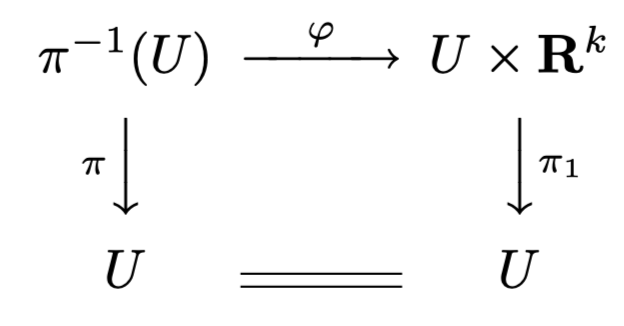
\includegraphics[width=0.25\textwidth]{Figs/1.png}
    % \caption{local trivialization. $U$ is on $M$.}
    \label{fig:dfadg3q}
\end{figure}
    (where $\pi_1$ is the projection onto the first factor).
   \item With $U$ and $\varphi$ as above, for each $q \in U$, the restriction $\left.\varphi\right|_{E_{q}}: E_{q} \rightarrow \{p\}\times\mathbf{R}^{k}\cong \mathbf{R}^{k}$ is a \tb{linear isomorphism}.
\end{enumerate}
\end{defa}
\begin{exma}
The \tb{tangent bundle} $TM$ of a smooth manifold $M$, which is just the disjoint union of the tangent spaces $T_{p} M$ for all $p \in M$, and the \tb{cotangent bundle} $T^{*} M$, which is the disjoint union of the cotangent spaces $T_{p}^{*} M=\left(T_{p} M\right)^{*}$. Another example is the \tb{normal bundle} to a submanifold $M \subset \mathbf{R}^{n}$, whose fiber at each point is the normal space $N_{p} M$, the orthogonal complement of $T_{p} M$ in $\mathbf{R}^{n}$.
\begin{figure}[h]
    \begin{center}
        \btik
            \draw[thick] (0,0) ellipse (1.25 and 0.5);
            \draw[thick] (-1.25,0) -- (-1.25,-4);
            \draw[thick] (-1.25,-4) arc (180:360:1.25 and 0.5);
            \draw[thick] (1.25,-4) -- (1.25,0);  
            \draw[dashed] (0,-2.3) ellipse (1.25 and 0.5); 
            \draw[blue, thick] (1,-4.3) .. controls (-0.5,-3.5) and (1,-2.5) .. (0.8,-1.8) .. controls (0.5, -1) ..  (0.5, -0.45);
            \draw[green, thick] (-0.7,-4.4) .. controls (0.5,-3.5) and (-1.2,-1.5) ..(-0.8, -0.4);
            \node at (-0.5, -3) {\large $p$};
            \node at (0.7, -3) {\large $q$};
            \node at (1.55,-2.3) {\large $\cM$};
            \node at (1, -0.7) {\large $E$};
            \fill [gray,opacity=0.2] (-1.25,0) -- (-1.25,-4) arc (180:360:1.25 and 0.5) -- (1.25,0) arc (0:180:1.25 and -0.5);
            \fill[gray, opacity=0.1] (0,0) ellipse (1.25 and 0.5);
        \etik
    \caption{Example of a bundle and fibre. The total space, $E$, is the surface of the cylinder and the base space, $\cM$, is the ring. The bundle is the triplet consisting of $E$, $M$ and a smooth, surjective projection map $\pi: E\to M$. The preimage of the the point $p$ w.r.t. the \tb{projection map} $\pi$ is the green line --- that is $\pi$ maps every point on the green line to $p$ --- known as the fibre over $p$. Similarly the blue line is the fibre over $q$. The \tb{section} w.r.t. $p$, $\sigma_p : M \to E$, maps $p$ to a point within its fibre (a point on the green line). A map $\tau : M\to E$ which maps $p$ to a point in $q$'s fibre (the blue line) is \textit{not} a section, as $(\pi \circ \tau)(p) = q \neq p$. The complete section is the set of points formed by taking one point from each fibre.}
    \label{fig:Bundlefibre}
    \end{center}
\end{figure}
\end{exma}
It frequently happens that we are given a collection of vector spaces, one for each point in a manifold, that we would like to "glue together" to form a vector bundle.  As the next lemma shows, all we need to do is to exhibit the maps that we wish to consider as local trivializations and check that they overlap correctly.
\begin{lema}\label{eq:ddsafa}
Let $M$ be a smooth manifold, $E$ a \tb{set}, and $\pi: E \rightarrow M$ a surjective map. Suppose we are given an open covering $\left\{U_{\alpha}\right\}$ of $M$ together with bijective maps $\varphi_{\alpha}: \pi^{-1}\left(U_{\alpha}\right) \rightarrow U_{\alpha} \times \mathbf{R}^{k}$ satisfying $\pi_{1} \circ \varphi_{\alpha}=\pi$, such that whenever $U_{\alpha} \cap U_{\beta} \neq \emptyset$, the composite map
\begin{align}
\varphi_{\alpha} \circ \varphi_{\beta}^{-1}: U_{\alpha} \cap U_{\beta} \times \mathbf{R}^{k} \rightarrow U_{\alpha} \cap U_{\beta} \times \mathbf{R}^{k}\label{eq:dfdfad}
\end{align}
is of the form
\begin{align*}
\varphi_{\alpha} \circ \varphi_{\beta}^{-1}(p, v)=(p, \tau(p) v) \text {, where } v \in \mathbf{R}^k
\end{align*}
for some smooth map $\tau: U_{\alpha} \cap U_{\beta} \rightarrow G L(k, \mathbf{R})$. Then $E$ has a unique structure as a smooth $k$-dimensional vector bundle over $M$ for which the maps $\varphi_{\alpha}$ are local trivializations.
\end{lema}
\begin{proof}
Step 1). Assign fiber a vector space structure: 
 For each $p \in M$, let $E_{p}=\pi^{-1}(p)$. If $p \in U_{\alpha}$, observe that the map $\left(\varphi_{\alpha}\right)_{p}: E_{p} \rightarrow\{p\} \times \mathbf{R}^{k}$ obtained by restricting $\varphi_{\alpha}$ is a bijection. We can \textit{define a vector space structure on $E_{p}$ by declaring this map to be a linear isomorphism.} This structure is well defined, since for any other set $U_{\beta}$ containing $p$, \cref{eq:dfdfad} guarantees that $\left(\varphi_{\alpha}\right)_{p} \circ\left(\varphi_{\beta}\right)_{p}^{-1}=\tau(p)$ is an isomorphism.

Step 2). Assign $E$ a smooth manifold structure from manifold $M$: 
Shrinking the sets $U_{\alpha}$ on manifold $M$ and taking more of them if necessary, we may assume each of them is diffeomorphic to some open set $\widetilde{U}_{\alpha} \subset \mathbf{R}^{n}$. Appending $\varphi_{\alpha}$ with such a diffeomorphism, we get a bijection $\pi^{-1}\left(U_{\alpha}\right) \rightarrow \widetilde{U}_{\alpha} \times \mathbf{R}^{k}$, which we can use as a coordinate chart for $E$. Because \cref{eq:dfdfad} shows that the $\varphi_{\alpha}$ s overlap smoothly, these charts determine a locally Euclidean topology and a smooth manifold structure on $E$.  Smooth is because the derivative of $\varphi_{\alpha} \circ \varphi_{\beta}^{-1}$ is $\big(\begin{smallmatrix}
  I & 0\\
  0 & \tau'
\end{smallmatrix}\big)$, so $\varphi_{\alpha} \circ \varphi_{\beta}^{-1}$ is smooth. It is immediate that each map $\varphi_{\alpha}$ is a diffeomorphism with respect to this smooth structure, and the rest of the conditions for a vector bundle follow automatically.
\end{proof} 
\begin{defa}\bfs{transition functions}
The smooth $G L(k, \mathbf{R})$-valued maps $\tau$ of the preceding lemma are called \tb{transition functions} for $E$.
\end{defa}
As an illustration, we show how to apply this construction to the tangent bundle.
\begin{cora}\bfs{construction of the tangent bundle}\label{cor:dhfdaafd}
 Given a coordinate chart $\left(U,\left(x^{i}\right)\right)$ for $M$, any tangent vector $V \in T_{x} M$ at a point $x \in U$ can be expressed in terms of the coordinate basis as $V=v^{i} \partial / \partial x^{i}$ for some $n$-tuple $v=\left(v^{1}, \ldots, v^{n}\right)$. Define a bijection $\varphi: \pi^{-1}(U) \rightarrow U \times \mathbf{R}^{n}$ by sending $V \in T_{x} M$ to $(x, v)$. Where two coordinate charts $\left(x^{i}\right)$ and $\left(\tilde{x}^{i}\right)$ overlap, the respective coordinate basis vectors are related by
\begin{align*}
\frac{\partial}{\partial x^{i}}=\frac{\partial \tilde{x}^{j}}{\partial x^{i}} \frac{\partial}{\partial \tilde{x}^{j}},
\end{align*}
and therefore the same vector $V$ is represented by
\begin{align*}
V=\tilde{v}^{j} \frac{\partial}{\partial \tilde{x}^{j}}=v^{i} \frac{\partial}{\partial x^{i}}=v^{i} \frac{\partial \tilde{x}^{j}}{\partial x^{i}} \frac{\partial}{\partial \tilde{x}^{j}} .
\end{align*}
This means that $\tilde{v}^{j}=v^{i} \partial \tilde{x}^{j} / \partial x^{i}$, so the corresponding local trivializations $\varphi$ and $\tilde{\varphi}$ are related by
\begin{align*}
\widetilde{\varphi} \circ \varphi^{-1}(x, v)=\widetilde{\varphi}(V)=(x, \tilde{v})=(x, \tau(x) v),
\end{align*}
where $\tau(x)$ is the $G L(n, \mathbf{R})$-valued function $\partial \tilde{x}^{j} / \partial x^{i}$. It is now immediate from \cref{eq:ddsafa} that these are the local trivializations for a vector bundle structure on $TM$.
\end{cora}
\begin{defa}\bfs{standard coordinates for the tangent bundle}
It is useful to note that this construction actually gives explicit coordinates $\left(x^{i}, v^{i}\right)$ on $\pi^{-1}(U)$, which we will refer to as standard coordinates for the tangent bundle.
\end{defa}
\begin{defa}\bfs{section; smooth section}
If $\pi: E \rightarrow M$ is a vector bundle over $M$, a section of $E$ is a map $F: M \rightarrow$ $E$ such that $\pi \circ F=Id_{M}$, or, equivalently, $F(p) \in E_{p}$ for all $p$. It is said to be a smooth section if it is smooth as a map between manifolds.
\end{defa}
\begin{defa}\bfs{local frame}
A local frame for $E$ is a finite sequence $\left(\sigma_{1}, \ldots, \sigma_{k}\right)$ of smooth sections of $E$ over $U$ such that $\left(\left.\sigma_{1}\right|_{p}, \ldots,\left.\sigma_{k}\right|_{p}\right)$ form a basis for $E_{p}$ at each point $p \in U . "$
\end{defa}
\begin{cora}\bfs{from local trivialization to local frame}
 Let $\psi: \pi^{-1}(U) \rightarrow U \times \mathbb{R}^{k}$ be a local trivialization and $\left\{e_{1}, \ldots, e_{k}\right\}$ the canonical basis of $\mathbb{R}^{k}$. Define $r_{i}: U \rightarrow E$ by $r_{i}(p):=\psi^{-1}\left(p, e_{i}\right)$ for all $p \in U$. Then $\left\{r_{1}, \ldots, r_{k}\right\}$ is the desired frame.
\end{cora}
\begin{cora}\bfs{from  local frame to local trivialization}
 If $\left(\sigma_{1}, \ldots, \sigma_{k}\right)$ is a local frame for a vector bundle $E$ over an open set $U \subset M$, let $\phi$ : $U \times \mathbf{R}^{k} \rightarrow$ $\pi^{-1}(U)$ be the map $\phi(p, x)=\left.x^{i} \sigma_{i}\right|_{p}$. Show that $\phi^{-1}$ is a local trivialization of $E$.
\end{cora}

\begin{lema}
Let $F: M \rightarrow E$ be a section of a vector bundle. $F$ is smooth if and only if the components $F^i$ of $F$ in terms of any smooth local frame $\left\{\sigma_{i}\right\}$ on an open set $U \in M$ depend smoothly on $p \in U$.
\end{lema}
\begin{proof}
 Let $\psi: \pi^{-1}(U) \rightarrow U \times \mathbb{R}^{k}$ be the local trivialization associated with the local frame $\left(\sigma_{i}\right)$. Because $\psi$ is a diffeomorphism, $F$ is smooth on $U$ if and only if the composite map $\psi \circ F$ is smooth on $U$. It is straightforward to check that $\psi \circ F(p)=\left(p,\left(F^{1}(p), \ldots, F^{k}(p)\right)\right)$, where $\left(F^{i}\right)$ are the component functions of $F$ with respect to $\left(\sigma_{i}\right)$, so $\psi \circ F$ is smooth if and only if the component functions $F^{i}$ are smooth.
\end{proof}
\subsection{Tangent Bundle of Smooth Manifold}
Of course we could construct tangent bundle according to \cref{cor:dhfdaafd} by formulation. However, here we present the construction in a more intuitive way.

$\bullet$ \tb{step 1: a set}

Let $(\cM,\cO,\cA)$ be a smooth manifold. We define the \textbf{tangent bundle} as the bundle whose base space is our smooth manifold and whose \tb{total space has the set} \footnote{We shall make this into a smooth manifold below.} 
\begin{align*}
    T\cM := \bigcup^{\bullet}_{p\in\cM} T_p\cM,
\end{align*}
where the dot means `disjoint union'. The \tb{projection map} is given by
\begin{align*}
    \pi : X \mapsto p,
\end{align*}
where $p$ is the \textit{unique} point such that $X\in T_p\cM$.

It is important that we take the disjoint union above as this allows us to identify each vector with its base point $p$. It is because we take the disjoint union that we can say the \textit{unique} point; and the projection is surjective as we took the union over all $p\in\cM$ and so we hit every element in $\cM$. 

$\bullet$ \tb{step 2: a topological manifold}

We now need to make $T\cM$ into a smooth manifold, in such a way that $\pi:T\cM \to \cM$ is a smooth map. So we need to define a topology on $T\cM$, and here we choose the \tb{weak topology} such that $\pi$ is continuous (as continuity is needed for smoothness):
\begin{align*}
    \cO_{T\cM} := \{ \preim_{\pi}(U) \, | \, U\in\cO\}
\end{align*}

$\bullet$ \tb{step 3: manifold with atlas}

So far we have a topological manifold $(T\cM,\cO_{T\cM})$ and a continuous map $\pi$ to a smooth manifold $(\cM,\cO,\cA)$. We now need to define a $C^{\infty}$-atlas for $(T\cM,\cO_{T\cM})$ in such a way that our map becomes smooth. As with the topology, we are going to construct this atlas from $\cA$. 

We know that $X\in T\cM$ is described by \tb{two pieces of information}: it is a vector and it has a base point. We can easily obtain the coordinates of the base point by simply projecting $X$ down using $\pi$ and then using our atlas on $\cM$ to find its coordinates. For the vector part, we have a chart on $\cM$ and so we can induce a chart on the tangent space and decompose $X$ as 
\begin{align*}
    X =: X^i_{(x)}\frac{\p}{\p x^i}.
\end{align*}
We have
\begin{align*}
    X^i_{(x)} = (dx^i)_{\pi(X)}(X).
\end{align*}
So we construct the atlas
\begin{align*}
    \cA_{T\cM} := \{ (TU,\xi_x) \, | \, (U,x) \in\cA\},
\end{align*}
where
\begin{align*}
    \xi_x : TU \to \R^{2\cdot\dim\cM},
\end{align*}
given by
\begin{align*}
    \xi_x(X) = \big( \underbrace{(x^1\circ\pi)(X), ... , (x^d\circ \pi)(X)}_{(U,x)\text{-coordinate of }\pi(X)}, \underbrace{(dx^1)_{\pi(X)}(X), ... , (dx^d)_{\pi(X)}(X)}_{\text{Vector components w.r.t. } (U,x)}\big)
\end{align*}
We also need the inverse map:
\begin{align*}
    \xi_x^{-1} : \R^{2\cdot\dim\cM} \to TU.
\end{align*}
With a bit of thought it is clear that it must satisfy 
\begin{align*}
    \xi_x^{-1}(\a^1,...,\a^d,\beta_1,...,\beta^d) := \beta^i \bigg(\frac{\p}{\p x^i}\bigg)_{x^{-1}(\a^1,...,\a^d)} = \beta^i \bigg(\frac{\p}{\p x^i}\bigg)_{\pi(X)}.
\end{align*}
Now we need to check that these maps are smooth (as we need a smooth atlas). Consider another chart $(V,y)$ with $V\cap U\neq\emptyset$, we have
\begin{align*}
    \begin{split}
        \big(\xi_y\circ \xi_x^{-1}\big) (\a^1,...,\a^d,\beta^1,...,\beta^d) & := \xi_y \bigg( \beta^m \bigg(\frac{\p}{\p x^m}\bigg)_{\pi(X)}\bigg) \\
        & = \Bigg(..., (y^i\circ \pi) \bigg(\beta^i \bigg(\frac{\p}{\p x^i}\bigg)_{\pi(X)}\bigg),..., ..., (dy^i)_{\pi(X)}\bigg[\bigg(\beta^m \bigg(\frac{\p}{\p x^m}\bigg)_{\pi(X)}\bigg)\bigg], ...\Bigg) \\
        & = \Bigg(..., (y^i\circ x^{-1})(\a^1,...,\a^d), ..., ..., \beta^m \bigg(\frac{\p y^i}{\p x^m}\bigg)_{\pi(X)}, ...\Bigg) \\
        & = \Big(..., (y^i\circ x^{-1})(\a^1,...,\a^d), ..., ..., \beta^m \p_m \big(y^i\circ x^{-1}\big)\big|_{(\a^1,...,\a^d)}, ... \Big),
    \end{split}
\end{align*}
where to go to the third line we have used the fact that $\pi(X) = p = x^{-1}(\a^1,...,\a^d)$ and to get to the last line we have used the definition for the derivative fraction along with $(x\circ\pi)(X) = x(p) = (\a^1,...,\a^d)$. Now $(y^i\circ x^{-1})$ is smooth because $\cA$ is smooth and so the above result is smooth. We therefore have a smooth atlas $\cA_{T\cM}$.

\bd\bfs{Tangent Bundle}
    The triple $(T\cM,\pi,\cM)$ is a bundle, known as the \textbf{tangent bundle}. 
\ed 
\bex 
    Let $\cM=S^1$ (a circle) and let the fibres just run straight up and down. The further up/down the fibre one goes, the greater the value of the vector, with going downwards corresponding to placing a minus sign in front of the vector.

    $U$ here is a small part of the circle and is mapped by $x$ to a open interval in the real line. $TU$ is the set of fibres that run through $U$. These are mapped via $\xi_x$ to $\R^2$ in the following way. Consider a point on one of the fibres, call it $X$. The horizontal axis value in the $\R^2$ chart is given by the value the base point $p=\pi(X)\in\cM$ takes in the $\R$ chart, as mapped by $x$. The vertical value in the $\R^2$ chart is just given by the size of the vector (as it is only one-dimensional so the component is the size) and is plotted accordingly.
    \begin{center}
        \btik 
            \draw[thick] (0,0) ellipse (1.25 and 0.5);
            \draw[thick] (-1.25,0) -- (-1.25,-4);
            \draw[thick] (-1.25,-4) arc (180:360:1.25 and 0.5);
            \draw[thick] (1.25,-4) -- (1.25,0);  
            \draw[dashed] (0,-2.3) ellipse (1.25 and 0.5); 
            \fill [gray,opacity=0.2] (-1.25,0) -- (-1.25,-4) arc    (180:360:1.25 and 0.5) -- (1.25,0) arc (0:180:1.25 and -0.5);
            \fill[gray, opacity=0.1] (0,0) ellipse (1.25 and 0.5);
            \node at (1.55,-2.3) {\large $\cM$};
            \node at (1, -0.7) {\large $E$};
            %
            \draw[thick, blue] (-0.5,-4.45) -- (-0.5, -0.45);
            \draw[thick, blue] (-0.6,-4.45) -- (-0.6, -0.45);
            \draw[thick, blue] (-0.7,-4.4) -- (-0.7, -0.4);
            \draw[thick, blue] (-0.8,-4.4) -- (-0.8, -0.4);
            \draw[thick, blue] (-0.9,-4.35) -- (-0.9, -0.35);
            \draw[thick, blue] (-1,-4.33) -- (-1, -0.3);
            \draw[fill=black] (-0.6,-1) circle [radius=0.05cm];
            \node at (-0.7,-0.1) {\textcolor{blue}{\large{$TU$}}};
            %
            \draw[ultra thick, red] (0,-2.3) [partial ellipse=215:248:1.25cm and 0.5cm];
            \node at (-0.3, -2.5) {\textcolor{red}{\large{$U$}}};
            %
            \draw[->] (-6,-2.5) -- (-3.5,-2.5);
            \draw[ultra thick, red] (-5.5,-2.5) -- (-4,-2.5);
            \draw[thick, red, fill=white] (-5.5,-2.5) circle [radius=0.08cm];
            \draw[thick, red, fill=white] (-4,-2.5) circle [radius=0.08cm];
            \node at (-3.25,-2.5) {\large{$\R$}};
            \draw[->, red] (-0.7, -2.7) .. controls (-1.9,-3) and (-3.2,-3) .. (-4.75,-2.7) node[label={below:\large $x$}, midway] {};
            % 
            \draw[->] (3.5,-1.5) -- (7,-1.5);
            \draw[->] (3.6,-3) -- (3.6,0);
            \draw[thick, blue] (4,-3) -- (4,0);
            \draw[thick, blue] (4.5,-3) -- (4.5,0);
            \draw[thick, blue] (5,-3) -- (5,0);
            \draw[thick, blue] (5.5,-3) -- (5.5,0);
            \draw[thick, blue] (6,-3) -- (6,0);
            \draw[thick, blue] (6.5,-3) -- (6.5,0);
            \draw[fill=black] (6,-0.5) circle [radius=0.05];
            \draw[ultra thick, red] (4,-1.5) -- (6.5,-1.5);
            \node at (7,-0.5) {\large{$\R^2$}};
            \draw[->, blue] (-0.3, -1) .. controls (0.9,-1.5) and (2.1,-0.5) .. (3.3, -1) node[label={above:\large $\xi_x$}, midway, xshift =0.5cm] {};
        \etik 
    \end{center}
\eex 

\subsection{Vector Fields}
Given tangent bundle, we could then define smooth vector field.
\bd[Smooth Vector Field]
    A \textbf{smooth vector field} is a \textit{smooth section} on the tangent bundle. That is 
    \begin{align*}
        \chi : \cM\to T\cM, \qquad \pi\circ \chi = Id{\cM}.
    \end{align*}
\ed 
\begin{rema}
The smooth part of the above definition is what all the work was for. Intuitively when we think of a vector field (a vector at each point) we see a smooth vector field, i.e. one where the vectors appear to naturally flow from one to another, rather then just pointing randomly at each point.
\end{rema}
\subsection{The $C^{\infty}(\cM)$-Module}
So far we have a definition for a smooth vector field, but we have no way of adding them together or scaling them in any way. The addition is straight forward, just add the vectors in the tangent spaces together and take the result to be the new vector at that point. What about scaling? We need a new way to define the addition and scaling by using the scalar fields (smooth functions).

 Recall the definition
\begin{align*}
    C^{\infty}(\cM) := \{f:\cM\to\R \, | \, f \text{ is a smooth function}\}.
\end{align*}
It is possible that a non-vanishing\footnote{That is does not map every point $p\in\cM$ to $0\in\R$.} element of $C^{\infty}(\cM)$ can vanish at some points, we therefore can only get a \textit{commutative, unital ring}. If we build on top of this, we get a \textit{module} for the space of all smooth sections. 

\bd\bfs{The $C^{\infty}(\cM)$-Module, $\Gamma T\cM$}
    The triple $(\Gamma T\cM,\oplus,\odot)$ is a $C^{\infty}(\cM)$-module where 
    \begin{align*}
        \Gamma T\cM := \{ \chi :\cM \to T\cM \, | \, \text{smooth section}\},
    \end{align*}
    and 
    \begin{align*}
        \begin{split}
            (\chi\oplus \widetilde{\chi})\la f\ra & := \chi\la f\ra + \widetilde{\chi}\la f\ra, \\
            (g\odot \chi)\la f\ra & = g \cdot \chi\la f \ra, 
        \end{split}
    \end{align*}
    where $+/\cdot$ are the addition/multiplication on $C^{\infty}(\cM)$. See below for definition of $\chi\la f\ra$.
\ed 
\begin{rema}
A smooth vector field is a map $\chi:\cM\to T\cM$, so how does it act on a scalar field? The answer is obviously through the vectors that make up $\chi$: 
\begin{align*}
    \chi\la f\ra\big|_{p} := \big(\chi(p)\big)(f).
\end{align*}
That is, we first evaluate $\chi(p)$, which gives us \textit{the} $X\in T_p\cM$, and then we let this act on the scalar field, giving a real number. We do this for every point $p\in\cM$ and so get a map that associates to each point a real number, this is a scalar field. In other words we can think of smooth vector fields as maps 
\begin{align*}
    \chi : C^{\infty}(\cM) \lmap C^{\infty}(\cM).
\end{align*}
\end{rema}
\begin{rema}\bfs{Leibniz rule}
 \begin{align*}
        \chi \la f\bullet g\ra = f\bullet \chi\la g \ra + \chi\la f\ra \bullet g,
    \end{align*}
    where $\bullet : C^{\infty}(\cM)\times C^{\infty}(\cM) \to C^{\infty}(\cM)$ is the multiplication on the ring. This property is known as the \textbf{Leibniz rule}. Note for partial differential equations it is the familiar product rule. Later we will define it for general case in \textit{connection}.
\end{rema}

\begin{rema}\bfs{global frame}
 In general, we \textit{cannot} simply take the subset 
\begin{align*}
    \{\chi_1,...,\chi_d\} \se \Gamma T\cM
\end{align*}
such that any other $\chi\in\Gamma T\cM$ can be expressed as a linear combination of this subset
\begin{align*}
    \chi = f^i \odot \chi_i.
\end{align*}
In other words, in most case, we only have local frames but not global frames. 
This failure to define a global, nowhere vanishing, smooth vector field is related to the fact that we can't chart the space using only a single chart. 
\end{rema}

\bex 
    Consider a ball with a smooth vector field over it. If we imagine this smooth vector field as hairs sticking out of the ball, the idea of having a globally defined nowhere vanishing smooth vector field, would be to `comb' the hairs flat to the surface. That is, we want all of the vectors to lie in the tangent spaces and not `stick straight out'.
    
    However, in order to do this, we would have to remove some of the hairs: for example in the diagram drawn below, the hair at the top and bottom would have to `vanish' if we wanted the ball to be smooth.   The fact that the vector field is not defined globally means that it can not possibly be a basis element. 
    \begin{center}
        \btik
            \draw[thick] (-4,0) circle (2.5cm);
            \draw[thick, blue] (-4,2.5) .. controls (-4.5,2.88) and (-3.5,3.17) .. (-4, 3.5) node[circle, fill=black, inner sep=1pt] at (-4,2.5) {};
            \draw[thick, blue, rotate around={60:(-4,0)}] (-4,2.5) .. controls (-4.5,2.88) and (-3.5,3.17) .. (-4, 3.5) node[circle, fill=black, inner sep=1pt] at (-4,2.5) {};
            \draw[thick, blue, rotate around={120:(-4,0)}] (-4,2.5) .. controls (-4.5,2.88) and (-3.5,3.17) .. (-4, 3.5) node[circle, fill=black, inner sep=1pt] at (-4,2.5) {};
            \draw[thick, blue, rotate around={180:(-4,0)}] (-4,2.5) .. controls (-4.5,2.88) and (-3.5,3.17) .. (-4, 3.5) node[circle, fill=black, inner sep=1pt] at (-4,2.5) {};
            \draw[thick, blue, rotate around={-60:(-4,0)}] (-4,2.5) .. controls (-4.5,2.88) and (-3.5,3.17) .. (-4, 3.5) node[circle, fill=black, inner sep=1pt] at (-4,2.5) {};
            \draw[thick, blue, rotate around={-120:(-4,0)}] (-4,2.5) .. controls (-4.5,2.88) and (-3.5,3.17) .. (-4, 3.5) node[circle, fill=black, inner sep=1pt] at (-4,2.5) {};
            \draw[thick, blue, rotate around={22.5:(-4,0)}, yshift = -1.5cm] (-4,2.5) .. controls (-4.5,2.88) and (-3.5,3.17) .. (-4, 3.5) node[circle, fill=black, inner sep=1pt] at (-4,2.5) {};
            \draw[thick, blue, rotate around={-67.5:(-4,0)}, yshift = -1.5cm] (-4,2.5) .. controls (-4.5,2.88) and (-3.5,3.17) .. (-4, 3.5) node[circle, fill=black, inner sep=1pt] at (-4,2.5) {};
            \draw[thick, blue, rotate around={20:(-4,0)}, yshift = -3cm, xshift=-1cm] (-4,2.5) .. controls (-4.5,2.88) and (-3.5,3.17) .. (-4, 3.5) node[circle, fill=black, inner sep=1pt] at (-4,2.5) {};
            \draw[thick, blue, rotate around={-17.5:(-4,0)}, yshift = -2.5cm] (-4,2.5) .. controls (-4.5,2.88) and (-3.5,3.17) .. (-4, 3.5) node[circle, fill=black, inner sep=1pt] at (-4,2.5) {};
            \draw[thick, blue, rotate around={-150.5:(-4,0)}, yshift = -1.5cm] (-4,2.5) .. controls (-4.5,2.88) and (-3.5,3.17) .. (-4, 3.5) node[circle, fill=black, inner sep=1pt] at (-4,2.5) {};
            %
            \draw[->, ultra thick] (-1,0) -- (1,0);
            %
            \draw[thick] (4,0) circle (2.5cm);
            \draw[thick, blue] (1.5,0) .. controls (3.1, -0.5) and (4.8,-0.5) .. (6.5,0);
            \draw[thick, blue] (1.75,1.15) .. controls (3.23,0.65) and (4.77,0.65) .. (6.25,1.15);
            \draw[thick, blue] (2.5,2) .. controls (3.5, 1.8) and (4.5,1.8) .. (5.5,2);
            \draw[thick, blue] (1.75,-1.15) .. controls (3.23,-1.65) and (4.77,-1.65) .. (6.25,-1.15);
            \draw[thick, blue] (2.5,-2) .. controls (3.5, -2.3) and (4.5,-2.3) .. (5.5,-2);
            \draw[thick, blue] (4,2.5) .. controls (3.5,2.88) and (4.5,3.17) .. (4, 3.5) node[circle, fill=black, inner sep=1pt] at (4,2.5) {};
            \draw[thick, blue, rotate around={180:(4,0)}] (4,2.5) .. controls (3.5,2.88) and (4.5,3.17) .. (4, 3.5) node[circle, fill=black, inner sep=1pt] at (4,2.5) {};
        \etik
    \end{center}
\eex
\begin{defa}\bfs{Covector Fields}
We can repeat everything we did in order to define the tangent bundle but instead starting from the cotangent space $(T^*\cM,+,\cdot)$. In doing this we get the cotangent bundle and smooth covector fields. Finally we get the $C^{\infty}(\cM)$-module $(\Gamma T^*\cM,\oplus,\odot)$ where 
\begin{align*}
    \Gamma T^*\cM := \{ \alpha : \cM \to T^*\cM \, | \, \text{smooth section}\}.
\end{align*}
\end{defa}

\bex 
    Recall we had the differential at a point $(df)_p : T_p\cM\lmap\R$. We now want to extend this to be over the whole manifold. We therefore define 
    \begin{align*}
        df : \Gamma T\cM \lmap C^{\infty}(\cM)
    \end{align*}
    by\footnote{We denote the action of $df$ on $X$ by a colon and the action of a vector field on a scalar field via angled brackets.} 
    \begin{align*}
        df : \chi := \chi \la f \ra.
    \end{align*}
    The linearity here is actually \tb{$C^{\infty}$-linear}. This is different to smooth vector fields, which are only $\R$-linear. That is for all $\chi,\Upsilon\in\Gamma T\cM$ and $g\in C^{\infty}(\cM)$,
    \begin{align*}
        \begin{split}
            df:(\chi \oplus \Upsilon) & = (df:\chi) + (df:\Upsilon) \\
            df : (g\odot \chi) & = g\cdot (df:\chi).
        \end{split}
    \end{align*}
\eex 

\subsection{Tensor Fields}

We have the smooth vector fields and the smooth covector fields. We can, therefore, now construct smooth \textit{tensor} fields. 

\bd[Smooth Tensor Field]
    A \textbf{smooth $(r,s)$-tensor field} is a $C^{\infty}(\cM)$ multilinear map 
    \begin{align*}
        T : \underbrace{\Gamma T^*\cM \times ... \times \Gamma T^*\cM}_{r\text{-terms}} \times \underbrace{\Gamma T\cM \times ... \times \Gamma T\cM}_{s{\text{-terms}}} \lmap C^{\infty}(\cM),
    \end{align*}
    or in the other notation 
    \begin{align*}
        T := \underbrace{\Gamma T\cM \otimes ... \otimes \Gamma T\cM}_{r\text{-terms}} \times \underbrace{\Gamma T^*\cM \otimes ... \otimes \Gamma T^*\cM}_{s{\text{-terms}}}.
    \end{align*}
\ed 
$\bullet$ \tb{local frame and local coframe}

Let $\left(E_{1}, \ldots, E_{n}\right)$ be any local frame for $T M$, that is, $n$ smooth vector fields defined on some open set $U$ such that $\left(\left.E_{1}\right|_{p}, \ldots,\left.E_{n}\right|_{p}\right)$ form a basis for $T_{p} M$ at each point $p \in U$. Associated with such a frame is the dual coframe, which we denote $\left(\varphi^{1}, \ldots, \varphi^{n}\right)$; these are smooth 1-forms satisfying $\varphi^{i}\left(E_{j}\right)=\delta_{j}^{i}$.  In particular, in terms of a coordinate frame $\left\{\partial_{i}\right\}$ and its dual coframe $\left\{d x^{i}\right\}, F$ has the coordinate expression
\begin{align*}
F_{p}=F_{i_{1} \ldots i_{k}}^{j_{1} \ldots j_{l}}(p) \partial_{j_{1}} \otimes \cdots \otimes \partial_{j_{l}} \otimes d x^{i_{1}} \otimes \cdots \otimes d x^{i_{k}} .
\end{align*}
\begin{lema}
It is easy to check that this map is multilinear over $C^{\infty}(M)$, that is, for any functions $f, g \in C^{\infty}(M)$ and any smooth vector or \tb{covector fields} $\alpha$, $\beta$,
\begin{align*}
F(\ldots, f \alpha+g \beta, \ldots)=f F(\ldots, \alpha, \ldots)+g F(\ldots, \beta, \ldots)
\end{align*}
\end{lema}
\section{Connection (Covariant Derivatives)}
Before we can define curvature on Riemannian manifolds, we need to study geodesics, the Riemannian generalizations of straight lines. It is tempting to define geodesics as curves that minimize length, at least between nearby points. However, this property turns out to be technically difficult to work with as a definition, so instead we’ll choose a different property of straight lines and generalize that.

A curve in Euclidean space is a straight line if and only if its acceleration is identically zero. This is the property that we choose to take as a defining property of geodesics on a Riemannian manifold. To make sense of this idea, we’re going to have to introduce a new object on manifolds, called a connection. It is essentially \tb{a coordinate-invariant set of rules for taking directional derivatives of vector fields.}

$\bullet$ \tb{Motivation:}
    \begin{figure}[ht]
    \centering
    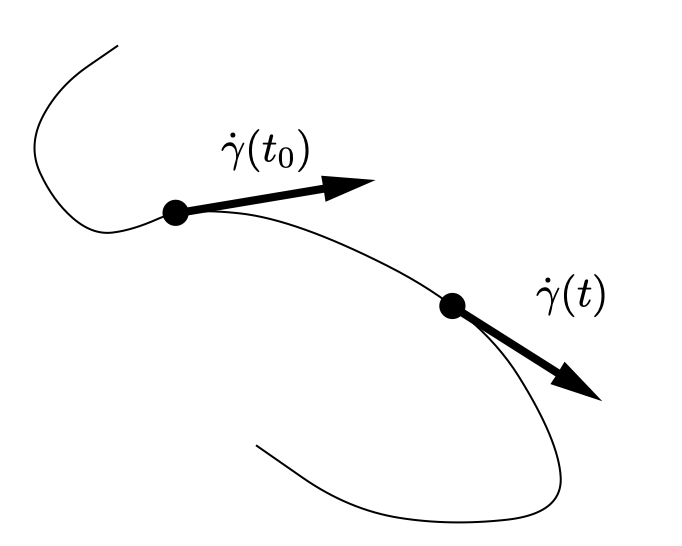
\includegraphics[width=0.3\textwidth]{Figs/2.png}
    \caption{issue of second derivative. $U$ is on $M$.}
    % \label{fig:dfadg3q}
\end{figure}
In many cases, we would like to study the acceleration vector $\ddot{\gamma}(t)$ of a velocity vector $\dot{\gamma}(t)$ of a curve $\gamma(t)$, 
The problem is this: If we wanted to make sense of $\ddot{\gamma}\left(t_{0}\right)$ by differentiating $\dot{\gamma}(t)$ with respect to $t$, we would have to write a difference quotient involving the vectors $\dot{\gamma}(t)$ and $\dot{\gamma}\left(t_{0}\right)$; but these live in different vector spaces $\left(T_{\gamma(t)} M\right.$ and $T_{\gamma\left(t_{0}\right)} M$ respectively), so it doesn't make sense to subtract them. We need a way to compare values of the vector field at different points, or, intuitively, to "connect" nearby tangent spaces. This is where a connection comes in: it will be an additional piece of data on a manifold, \tb{a rule for computing directional derivatives of vector fields}. (The velocity vector $\dot{\gamma}(t)$ is an example of a "vector field along a curve," a concept for which we will give a rigorous definition presently.) 

$\bullet$ \tb{Notation Discussion}

So far we have seen that a vector field $X$ can be used to provide a directional derivative $X\la f\ra$ of a function $f\in C^{\infty}(\cM)$. To remind ourselves that we are dealing with directional derivatives, we shall introduce a new notation 
\begin{align*} 
    \nabla_X f := X\la f\ra.
\end{align*} 
This seem like a massive notational overkill: we have three equivalent expressions,
\begin{align*}
    \nabla_X f = X\la f\ra = df:X.
\end{align*} 
However, although the evaluations are equal, the three objects are actually different as maps. That is
% For some reason overleaf was not having the \begin{align*} \end{align*} code here! That's why I've used \begin{equation*}
\begin{equation*}
    \begin{split}
        X : C^{\infty}(\cM) & \lmap C^{\infty}(\cM), \\
        df : \Gamma T\cM & \lmap C^{\infty}(\cM).
    \end{split}
\end{equation*}
What about $\nabla_X$, that as a map
\begin{align*} 
    \nabla_X : C^{\infty}(\cM) \lmap C^{\infty}(\cM),
\end{align*} 
appears to be exactly the same as $X$. This is true, but it turns out that we can actually extend the definition of $\nabla_X$ to be a map from a $(r,s)$-tensor field to a $(r,s)$-tensor field, which $X$ cannot. 

\subsection{Connection of Smooth Sections}
It turns out to be easiest to define a connection first as a way of differentiating sections of vector bundles. Later we will adapt the definition to the case of vector fields along curves.
\begin{defa}\bfs{connection of smooth sections; covariant derivative}
Let $\pi: E \rightarrow M$ be a vector bundle over a manifold $M$, and let $\mathcal{E}(M)$ denote the space of smooth sections of $E$. Let $\mathcal{T}(M)$ be the space of all vector fields.  A connection in $E$ is a map
\begin{align*}
\nabla: \mathcal{T}(M) \times \mathcal{E}(M) \rightarrow \mathcal{E}(M),
\end{align*}
written $(X, Y) \mapsto \nabla_{X} Y$, satisfying the following properties:
\begin{enumerate}[(a)]
    \item $\nabla_{X} Y$ is \tb{linear over $C^{\infty}(M)$ in $X$ }:
\begin{align*}
\nabla_{f X_{1}+g X_{2}} Y=f \nabla_{X_{1}} Y+g \nabla_{X_{2}} Y \quad \text { for } f, g \in C^{\infty}(M)
\end{align*}
\item $\nabla_{X} Y$ is \tb{linear over $\mathbf{R}$ in $Y$}:
\begin{align*}
\nabla_{X}\left(a Y_{1}+b Y_{2}\right)=a \nabla_{X} Y_{1}+b \nabla_{X} Y_{2} \quad \text { for } a, b \in \mathbf{R} ;
\end{align*}
\item $\nabla$ satisfies the following \tb{product rule}:
\begin{align*}
\nabla_{X}(f Y)=f \nabla_{X} Y+(X f) Y \quad \text { for } f \in C^{\infty}(M) \text {. }
\end{align*}
The symbol $\nabla$ is read "del," and $\nabla_{X} Y$ is called the covariant derivative of $Y$ in the direction of $X$.
\end{enumerate}
\end{defa}


Although a connection is defined by its action on global sections, it follows from the definitions that it is actually a local operator, as the next lemma shows.
\begin{lema}\bfs{locally defined I}\label{lem:ondfad}
If $\nabla$ is a connection in a bundle $E, X \in \mathcal{T}(M), Y \in \mathcal{E}(M)$, and $p \in M$, then $\left.\nabla_{X} Y\right|_{p}$ depends only on the values of $X$ and $Y$ in \tb{an arbitrarily small neighborhood of $p$}. More precisely, if $X=\widetilde{X}$ and $Y=\widetilde{Y}$ on a neighborhood of $p$, then $\left.\nabla_{X} Y\right|_{p}=\left.\nabla_{\tilde{X}} \widetilde{Y}\right|_{p}$.
\end{lema}
\begin{proof}
First consider $Y$. Replacing $Y$ by $Y-\tilde{Y}$, it clearly suffices to show that $\left.\nabla_{X} Y\right|_{p}=0$ if $Y$ vanishes on a neighborhood $U$ of $p$.

Choose a bump function $\varphi \in C^{\infty}(M)$ with support in $U$ such that $\varphi(p)=$ 1. The hypothesis that $Y$ vanishes on $U$ implies that $\varphi Y \equiv 0$ on all of $M$, so $\nabla_{X}(\varphi Y)=\nabla_{X}(0 \cdot \varphi Y)=0 \nabla_{X}(\varphi Y)=0$. Thus for any $X \in \mathcal{T}(M)$, the product rule gives
\begin{align*}
0=\nabla_{X}(\varphi Y)=(X \varphi) Y+\varphi\left(\nabla_{X} Y\right) .
\end{align*}
Now $Y \equiv 0$ on the support of $\varphi$, so the first term on the right is identically zero. We get that $\left.\nabla_{X} Y\right|_{p}=0$. The argument for $X$ is similar but easier.
\end{proof}
\begin{rema}
 The preceding lemma tells us that we can compute $\nabla_{X} Y$ at $p$ knowing only the values of $X$ and $Y$ near $p$. In fact, as the next lemma shows, we \tb{need only know the value of $X$ at $p$ itself.} This is different from the Lie derivative. And it is this local definition that makes connection over curve possible.
\end{rema}

\begin{lema}\bfs{locally defined II}\label{lem:oindfae}
With notation as in \cref{lem:ondfad}, $\left.\nabla_{X} Y\right|_{p}$ depends only on the values of $Y$ in a neighborhood of $p$ and the value of $X$ at $p$.
\end{lema}
\begin{proof}
By linearity, it suffices to show that $\left.\nabla_{X} Y\right|_{p}=0$ whenever $X_{p}=$ 0 . Choose a coordinate neighborhood $U$ of $p$, and write $X=X^{i} \partial_{i}$ in coordinates on $U$, with $X^{i}(p)=0$. Then, for any $Y \in \mathcal{E}(M)$,
\begin{align*}
\left.\nabla_{X} Y\right|_{p}=\left.\nabla_{X^{i} \partial_{i}} Y\right|_{p}=\left.X^{i}(p) \nabla_{\partial_{i}} Y\right|_{p}=0 .
\end{align*}
In the first equality, we used \cref{lem:ondfad}, which allows us to evaluate $\left.\nabla_{X} Y\right|_{p}$ by computing locally in $U$; in the second, we used linearity of $\nabla_{X} Y$ over $C^{\infty}(M)$ in $X$.
\end{proof}
Because of \cref{lem:oindfae}, we can write $\nabla_{X_{p}} Y$ in place of $\left.\nabla_{X} Y\right|_{p}$. This can be thought of as a directional derivative of $Y$ at $p$ in the direction of the vector $X_{p}$.
\subsubsection{Connection of Smooth Vector Field (Linear Connection)}
Now we specialize to connections in the tangent bundle of a manifold. 
\begin{defa}\bfs{connection of smooth vector field}
A (linear) connection on $(\cM,\cO,\cA)$ is a connection in $T M$, i.e., a map
\begin{align*}
\nabla: \mathcal{T}(\cM) \times \mathcal{T}(\cM) \rightarrow \mathcal{T}(\cM)
\end{align*}
satisfying properties (a)-(c) in the definition of a connection above.
\end{defa}

Next we examine how a linear connection appears in components. Let $\left\{E_{i}\right\}$ be a local frame for $T M$ on an open subset $U \subset M$. We will usually work with a coordinate frame $E_{i}=\partial_{i}$. For any choices of the indices $i$ and $j$, we can expand $\nabla_{\partial_{i}} \partial_{j}$ in terms of this same frame.
We can write these via the following definition.
\bd\bfs{Christoffel symbols; Connection Coefficient Functions}\label{def:kidnafe}
    Let $(\cM,\cO,\cA,\nabla)$ be an manifold and let $(U,x)\in\cA$. The \textbf{connection coefficient functions}, are the $(\dim \cM)^3$ many functions 
    \begin{align*} 
        \begin{split}
            \Gamma^i_{(x)jk} : U & \to \R \\
            p & \mapsto \bigg[dx^i :\bigg( \nabla_{\frac{\p}{\p x^k}} \frac{\p}{\p x^j}\bigg)\bigg]_p.
        \end{split}
    \end{align*}
\ed 

The following lemma shows that the action of the connection $\nabla$ on $U$ is completely determined by its Christoffel symbols.
\begin{lema}\label{lem:donafadf}
Let $\nabla$ be a linear connection, and let $X, Y \in \mathcal{T}(U)$ be expressed in terms of a local frame by $X=X^{i} \partial_{i}, Y=Y^{j} \partial_{j}$. Then
\begin{align*} 
    (\nabla_XY)^i = X\la Y^i\ra + X^jY^k \Gamma^i_{(x)kj}.
\end{align*} 
\end{lema} 
\begin{proof}Just use the defining rules for a connection and compute:
\begin{align*} 
    \begin{split}
        \nabla_XY & = \nabla_{X^i\frac{\p}{\p x^i}}\bigg(Y^j\frac{\p}{\p x^j}\bigg) \\
        & = X^i \nabla_{\frac{\p}{\p x^i}} \bigg(Y^j\frac{\p}{\p x^j}\bigg) \\
        & = X^i \Big(\nabla_{\frac{\p}{\p x^i}}Y^j\Big) \frac{\p}{\p x^j} + X^i Y^j \bigg(\nabla_{\frac{\p}{\p x^i}}\frac{\p}{\p x^j}\bigg) \\
        & = X^i \frac{\p Y^j}{\p x^i} \frac{\p}{\p x^j} + X^iY^j \bigg(\nabla_{\frac{\p}{\p x^i}}\frac{\p}{\p x^j}\bigg) \\
        & = X\la Y^j\ra \frac{\p}{\p x^j} + X^kY^i \Gamma^j_{(x)ki} \frac{\p}{\p x^j}
    \end{split}
\end{align*} 
\end{proof} 

\paragraph{Existence of Connections }
So far, we have studied properties of connections, but have not produced any, so you might be wondering if they are plentiful or rare. In fact, they are quite plentiful, as we will show shortly. Let's begin with a trivial example: 
\begin{defa}\bfs{Euclidean connection}
On $\mathbf{R}^{n}$, define the Euclidean connection by
\begin{align*}
\bar{\nabla}_{X}\left(Y^{j} \partial_{j}\right)=\left(X (Y^{j})\right) \partial_{j}
\end{align*}
\end{defa}
\begin{rema}
 In other words, $\bar{\nabla}_{X} Y$ is just the vector field whose components are the \tb{ordinary directional derivatives of the components of $Y$ in the direction $X$.} It is easy to check that this satisfies the required properties for a connection, and that its \tb{Christoffel symbols in standard coordinates are all zero.} Indeed on any manifold covered by a single coordinate chart this is true.
\end{rema}
\begin{lema}
Suppose $M$ is a manifold covered by a single coordinate chart. There is a \tb{one-to-one correspondence between linear connections on $M$ and choices of $n^{3}$ smooth functions $\left\{\Gamma_{i j}^{k}\right\}$ on $M$}, by the rule
\begin{align*}
\nabla_{X} Y=\left(X^{i} \partial_{i} Y^{k}+X^{i} Y^{j} \Gamma_{i j}^{k}\right) \partial_{k}
\end{align*}
\end{lema}
\begin{rema}
 This is the ``iff'' extension of \cref{lem:donafadf}.  Easy to check.
\end{rema}

\begin{lema}
Every manifold admits a linear connection.
\end{lema}
\begin{proof}
Cover $M$ with coordinate charts $\left\{U_{\alpha}\right\}$; the preceding lemma guarantees the existence of a connection $\nabla^{\alpha}$ on each $U_{\alpha}$. Choosing a partition of unity $\left\{\varphi_{\alpha}\right\}$ subordinate to $\left\{U_{\alpha}\right\}$, we'd like to patch the $\nabla^{\alpha}$ s together by the formula
\begin{align*}
\nabla_{X} Y=\sum_{\alpha} \varphi_{\alpha} \nabla_{X}^{\alpha} Y
\end{align*}
Again, it is obvious by inspection that this expression is smooth, linear over $\mathbf{R}$ in $Y$, and linear over $C^{\infty}(M)$ in $X$. We have to be a bit careful with the product rule, though, since a linear combination of connections is not necessarily a connection. (You can check, for example, that if $\nabla^{1}$ and $\nabla^{2}$
are connections, neither $\frac{1}{2} \nabla^{1}$ nor $\nabla^{1}+\nabla^{2}$ satisfies the product rule.) By direct computation,
\begin{align*}
\begin{aligned}
\nabla_{X}(f Y) &=\sum_{\alpha} \varphi_{\alpha} \nabla_{X}^{\alpha}(f Y) \\
&=\sum_{\alpha} \varphi_{\alpha}\left((X f) Y+f \nabla_{X}^{\alpha} Y\right) \\
&=(X f) Y+f \sum_{\alpha} \varphi_{\alpha} \nabla_{X}^{\alpha} Y \\
&=(X f) Y+f \nabla_{X} Y
\end{aligned}
\end{align*}
\end{proof}

\subsubsection{Connection of Tensor Fields}
By definition, a linear connection on $M$ is a way to compute covariant derivatives of vector fields. In fact, any linear connection automatically induces connections on all tensor bundles over $M$, and thus gives us a way to compute covariant derivatives of any tensor field.
\begin{lema}
Let $\nabla$ be a \tb{linear connection} on $M$. There is a \tb{unique connection} in each tensor bundle $T_{l}^{k} M$, also denoted $\nabla$, such that the following conditions are satisfied.
\begin{enumerate}
    \item On $TM$, $\nabla$ agrees with the given connection.
    \item On $T^{0} M$ (i.e. $C^\infty(M)$), $\nabla$ is given by ordinary differentiation of functions:
\begin{align*}
\nabla_{X} f=X f
\end{align*}
\item $\nabla$ obeys the following product rule with respect to tensor products:
\begin{align*}
\nabla_{X}(F \otimes G)=\left(\nabla_{X} F\right) \otimes G+F \otimes\left(\nabla_{X} G\right)
\end{align*}
\item $\nabla$ commutes with all contractions: if $\operatorname{tr}$ denotes the trace on any pair of indices,
\begin{align*}
\nabla_{X}(\operatorname{tr} Y)=\operatorname{tr}\left(\nabla_{X} Y\right)
\end{align*}
\end{enumerate}
This connection satisfies the following additional properties:
\begin{enumerate}[(i)]
    \item $\nabla$ obeys the following product rule with respect to the natural pairing between a covector field $\omega$ and a vector field $Y$ :
\begin{align*}
\nabla_{X}\langle\omega, Y\rangle=\left\langle\nabla_{X} \omega, Y\right\rangle+\left\langle\omega, \nabla_{X} Y\right\rangle
\end{align*}
    \item For any $F \in \mathcal{T}_{l}^{k}(M)$, vector fields $Y_{i}$, and 1-forms $\omega^{j}$,
\begin{align*}
\begin{aligned}
\left(\nabla_{X} F\right)\left(\omega^{1}, \ldots, \omega^{l}, Y_{1}, \ldots, Y_{k}\right)=&X\left(F\left(\omega^{1}, \ldots, \omega^{l}, Y_{1}, \ldots, Y_{k}\right)\right) \\
&-\sum_{j=1}^{l} F\left(\omega^{1}, \ldots, \nabla_{X} \omega^{j}, \ldots, \omega^{l}, Y_{1}, \ldots, Y_{k}\right) \\
&-\sum_{i=1}^{k} F\left(\omega^{1}, \ldots, \omega^{l}, Y_{1}, \ldots, \nabla_{X} Y_{i}, \ldots, Y_{k}\right)
\end{aligned}
\end{align*}
\end{enumerate}
\end{lema} 
\begin{proof}Hint: Show that the defining properties imply (i) and (ii); then use these to prove existence and uniqueness.
i) gives the definition for covector field derivative w.r.t. vector field.
ii) gives the general case using both the vector and covector field derivative w.r.t. vector field. 
\end{proof}

Because the covariant derivative $\nabla_{X} Y$ of a vector field (or tensor field) $Y$ is linear over $C^{\infty}(M)$ in $X$, it can be used to construct another tensor field called the total covariant derivative, as follows.
\begin{lema}
If $\nabla$ is a linear connection on $M$, and $F \in \mathcal{T}_{l}^{k}(M)$, the map $\nabla F: \mathcal{T}^{1}(M) \times \cdots \times \mathcal{T}^{1}(M) \times \mathcal{T}(M) \times \cdots \times \mathcal{T}(M) \rightarrow C^{\infty}(M)$, given by
\begin{align*}
\nabla F\left(\omega^{1}, \ldots, \omega^{l}, Y_{1}, \ldots, Y_{k}, X\right)=\nabla_{X} F\left(\omega^{1}, \ldots, \omega^{l}, Y_{1}, \ldots, Y_{k}\right)
\end{align*}
defines $a\left(\begin{array}{c}k+1 \\ l\end{array}\right)$-tensor field.
\end{lema} 
\begin{proof}
This follows immediately from the tensor characterization lemma: $\nabla_{X} F$ is a tensor field, so it is multilinear over $C^{\infty}(M)$ in its $k+l$ arguments; and it is linear over $C^{\infty}(M)$ in $X$ by definition of a connection.
\end{proof} 
\begin{defa}\bfs{total covariant derivative}
The tensor field $\nabla F$ is called the total covariant derivative of $F$. 
\end{defa}
\begin{exma}\bfs{covariant Hessian}
For example, let $u$ be a smooth function on $M$. Then $\nabla u \in \mathcal{T}^{1}(M)$ is just the 1-form $d u$, because both tensors have the same action on vectors: $\langle\nabla u, X\rangle=$ $\nabla_{X} u=X u=\langle d u, X\rangle$. The 2-tensor $\nabla^{2} u=\nabla(\nabla u)$ is called the covariant Hessian of $u$.
\end{exma}
When we write the components of a total covariant derivative in terms of coordinates, we use a semicolon to separate indices resulting from differentiation from the preceding indices. Thus, for example, if $Y$ is a vector field written in components as $Y=Y^{i} \partial_{i}$, the components of the $\left(\begin{array}{l}1 \\ 1\end{array}\right)$-tensor field $\nabla Y$ are written $Y_{; j}^{i}$, so that
\begin{align*}
\nabla Y=Y_{; j}^{i} \partial_{i} \otimes d x^{j},
\end{align*}
with
\begin{align*}
Y_{; j}^{i}=\partial_{j} Y^{i}+Y^{k} \Gamma_{j k}^{i}
\end{align*}
\begin{rema}\bfs{explanation}
$\nabla_X Y$ gives a vector field (whose input is a covector field) for each $X$. That means $(\nabla_{\cdot} Y)(\cdot)$ will take two inputs,  one is covector field, and the other is vector field (at the position of low index $\nabla_{\cdot}$). So We have the $\left(\begin{array}{l}1 \\ 1\end{array}\right)$-tensor field. According to \cref{lem:donafadf}, we only need to consider input $\partial_j$ at the position of $X$, and get that 
\begin{align*} 
    (\nabla_{\partial_j}Y)^i = \partial_j\la Y^i\ra + Y^k \Gamma^i_{(x)kj}.
\end{align*} 
\end{rema}
More generally, the next lemma gives a formula for the components of covariant derivatives of arbitrary tensor fields.

\begin{lema}
Let $\nabla$ be a linear connection. The components of the total covariant derivative of a $\left(\begin{array}{l}k \\ l\end{array}\right)$-tensor field $F$ with respect to a coordinate system are given by
\begin{align*}
F_{i_{1} \ldots i_{k} ; m}^{j_{j_{1} \ldots j_{l}}}=\partial_{m} F_{i_{1} \ldots i_{k}}^{j_{1} \ldots j_{l}}+\sum_{s=1}^{l} F_{i_{1} \ldots i_{k}}^{j_{1} \ldots p \ldots j_{l}} \Gamma_{m p}^{j_{s}}-\sum_{s=1}^{k} F_{i_{1} \ldots p \ldots i_{k}}^{j_{1} \ldots j_{l}} \Gamma_{m i_{s}}^{p}
\end{align*}
\end{lema}

\subsubsection{New Structure on $(\cM,\cO,\cA)$ Required to Fix $\nabla$}
The question we want to answer is whether this is unique or whether different $\nabla$s will give the same result. In other words, how much freedom do we have in choosing $\nabla$? That is we can tell you exactly which $\nabla$ we are using by telling you the $\Gamma$s. 

Clearly, we have seen in \cref{def:kidnafe} and \cref{lem:donafadf} that  we need  $(\dim \cM)^3$ many functions as \textbf{connection coefficient functions} to fix the covariant derivative of a vector field on the chart domain $U\se\cM$. 
Now you might say `hold up we only know that this will give us the covariant derivative of a vector field, what about the covariant derivative of different tensors? We will surely need more and more terms to find them!' Luckily the answer is that we don't and it suffices to just know that $\Gamma$s. In order to see this, consider the following. 

If we wanted to work out the action on a covector basis element $dx^i$, we could do a similar thing to above and expand the result in the basis. That is
\begin{align*} 
    \nabla_{\frac{\p}{\p x^i}} dx^j = \Theta^j_{(x)ki} dx^k,
\end{align*} 
where the $\Theta$s are defined by this expression. \tb{We want to show that we can actually express these $\Theta$s in terms of the $\Gamma$s}. In order to do that, consider the following:
\begin{align*} 
    \begin{split}
        \nabla_{\frac{\p}{\p x^i}} \bigg( dx^j : \frac{\p}{\p x^k}\bigg) & = \Big(\nabla_{\frac{\p}{\p x^i}} dx^j\Big):\frac{\p}{\p x^k} + dx^j :\bigg(\nabla_{\frac{\p}{\p x^i}}\frac{\p}{\p x^k}\bigg) \\
       \nabla_{\frac{\p}{\p x^i}}\del^j_k & = \Theta^{j}_{(x)\ell i}dx^{\ell}:\frac{\p}{\p x^k} + dx^j : \bigg( \Gamma^{\ell}_{(x)ki} \frac{\p}{\p x^{\ell}}\bigg) \\
       0 & = \Theta^j_{(x)\ell i} \del^{\ell}_k + \Gamma^{\ell}_{(x)ki} \del^j_{\ell} \\
       \Theta^j_{(x)ki} & = - \Gamma^j_{(x)ki},
    \end{split}
\end{align*}
and so by giving the $\Gamma$s we can also tell you the action of the covariant derivative on a covector field.

We have the following mnemonic: `when it acts on a vector field, you get a plus sign, when it acts on a covector you have a minus sign.' Summarising, we have 
\begin{align*} 
    \begin{split}
        (\nabla_X Y)^i & = X\la Y^i\ra + \Gamma^i_{(x)jk} X^k Y^j, \\
        (\nabla_X \omega)_i & = X\la \omega_i \ra - \Gamma^j_{(x)ik} X^k \omega_j.
    \end{split}
\end{align*}

So what about \tb{higher order tensors}? The answer is obviously just to use the Leibniz rule. For example, for a $(1,2)$-tensor field $T$ we have 
\begin{align*} 
    {(\nabla_XT)^i}_{jk} = X\la {T^i}_{jk}\ra + \Gamma^i_{(x)m\ell} X^{\ell} {T^m}_{jk} - \Gamma^m_{(x)j\ell}X^{\ell} {T^i}_{mk} - \Gamma^m_{(x)k\ell} X^{\ell}{T^m}_{jm}.
\end{align*} 
Each term is the contribution from one of the indices on the left-hand side. You consider that index formula and you leave the remaining two untouched. 
\br 
\label{rem:GammasChange}\bfs{vanishing $\Gamma$s}
    We can use the $\Gamma$s to define what we mean by a Euclidean space. Let $\cM=\R^3$ be equipped with the standard topology $\cO_{st}$ and a smooth atlas $\cA$. We define the Euclidean space to be this smooth manifold equipped with a connection such that is is possible to find \tb{a} chart $(U,x)\in\cA$ such that 
    \begin{align*} 
        \Gamma^i_{(x)jk} = 0,
    \end{align*} 
    for all $i,j,k\in\{1,...,\dim\cM\}$. Note we say `it is possible to find \tb{a} chart' such that this happens. As we will see, just because the $\Gamma$s vanish in one chart does not mean they will vanish in another (that is, they are not tensors!).
\er 
\bnn\bfs{notation}
    \benr 
        \item From now on,  we shall drop the $(x)$ subscript on the $\Gamma$s in order to lighten notation.
        \item Again unless the context requires, we shall also use the notation 
        \begin{align*} 
            \nabla_i := \nabla_{\frac{\p}{\p x^i}}.
        \end{align*} 
    \een 
\enn 

\bd\bfs{Divergence of Vector Field}
    Let $X$ be a vector field on a smooth affine manifold $(\cM,\cO,\cA,\nabla)$. The \textbf{divergence} of $X$ is the function 
    \begin{align*} 
        \operatorname{div}X := (\nabla_i X)^i.
    \end{align*} 
\ed 

\bcl 
    The above definition is chart independent.
\ecl 

\subsubsection{Change of $\Gamma$s Under Change of Chart}\label{sec:iii}

So far we have defined the $\Gamma$s on $U\se\cM$, we obviously want to extend this to be a global definition on all of $\cM$. We do this by considering overlapping charts and require compatibility. 

Assume we have a affine manifold $(\cM,\cO,\cA,\nabla)$ and consider two charts $(U,x)$ and $(V,y)$ with $U\cap V \neq \emptyset$. We want to relate the $\Gamma$s in these charts. 
\begin{align} 
    \begin{split}
        \Gamma^i_{(y)jk} & := dy^i : \bigg( \nabla_{\frac{\p}{\p y^j}}\frac{\p}{\p y^k}\bigg) \\
        & = \frac{\p y^i}{\p x^q} dx^q : \bigg( \nabla_{\frac{\p x^p}{\p y^j}\frac{\p}{\p x^p}} \frac{\p x^s}{\p y^k}\frac{\p}{\p x^s}\bigg) \\
        & = \frac{\p y^i}{\p x^q} dx^q : \bigg( \frac{\p x^p}{\p y^j} \bigg[ \frac{\p}{\p x^p}\bigg\la\frac{\p x^s}{\p y^k}\bigg\ra \frac{\p}{\p x^s} + \frac{\p x^s}{\p y^k} \bigg(\nabla_{\frac{\p}{\p x^p}} \frac{\p}{\p x^s}\bigg)\bigg]\bigg) \\
        & = \frac{\p y^i}{\p x^q} dx^q : \bigg( \frac{\p x^p}{\p y^j} \bigg[ \frac{\p}{\p x^p}\bigg\la\frac{\p x^s}{\p y^k}\bigg\ra \frac{\p}{\p x^s} + \frac{\p x^s}{\p y^k} \Gamma^m_{(x)sp} \frac{\p}{\p x^m}\bigg]\bigg) \\
        & = \frac{\p y^i}{\p x^q} \frac{\p x^p}{\p y^j} \bigg( \frac{\p}{\p x^p}\bigg\la\frac{\p x^s}{\p y^k}\bigg\ra \del^q_s + \frac{\p x^s}{\p y^k} \Gamma^{m}_{(x)sp} \del^q_m\bigg) \\
        & = \frac{\p y^i}{\p x^q} \frac{\p x^p}{\p y^j} \frac{\p}{\p x^p}\bigg\la\frac{\p x^q}{\p y^k}\bigg\ra  +  \frac{\p y^i}{\p x^q} \frac{\p x^p}{\p y^j}\frac{\p x^s}{\p y^k} \Gamma^{q}_{(x)sp} \\
        & = \frac{\p y^i}{\p x^q} \frac{\p}{\p y^j}\bigg\la \frac{\p x^q}{\p y^k}\bigg\ra + \frac{\p y^i}{\p x^q} \frac{\p x^p}{\p y^j}\frac{\p x^s}{\p y^k} \Gamma^{q}_{(x)sp} \\
        & = \underbrace{\frac{\p y^i}{\p x^q} \frac{\p^2 x^q}{\p y^j\p y^k}}_{\textcolor{blue}{\text{a symmetric term}}} + \underbrace{\frac{\p y^i}{\p x^q} \frac{\p x^p}{\p y^j}\frac{\p x^s}{\p y^k} \Gamma^{q}_{(x)sp}}_{\msout{\text{antisymmetric term}}}
    \end{split}\label{eq:omeqrv}
\end{align} 
where to get to the penultimate line we have used the change of chart rule, that is\footnote{This is an important step as we need both the derivatives to be w.r.t. the same chart label $(y)$ in order for us to be able to use Schwartz's rule for switching the differentiation order. }
\begin{align*} 
    \frac{\p x^p}{\p y^j}\frac{\p}{\p x^p} = \frac{\p}{\p y^j},
\end{align*} 
and where we have introduced the notation\footnote{Obviously this notation is just that for partial derivatives, but recall that our fractions $\frac{\p f}{\p x^i}$ don't mean partial derivative, it means the expression we defined before.} 
\begin{align*} 
    \frac{\p^2 x^q}{\p y^j\p y^k} := \frac{\p}{\p y^j} \bigg\la \frac{\p x^q}{\p y^k}\bigg\ra.
\end{align*} 
\begin{rema}
Previously, we made an mistake to claim the second term is antisymmetric. This is not correct. We can only get that the first term is symmetric. Imaging you have a symmetric $\Gamma$, that does not meaning under any change of coordinates you only have the first term.
\end{rema}
\begin{rema}
 Note that if the expression was simply 
\begin{align*} 
    \Gamma^i_{(y)jk} = \frac{\p y^i}{\p x^q} \frac{\p x^p}{\p y^j}\frac{\p x^s}{\p y^k} \Gamma^{q}_{(x)sp},
\end{align*} 
we would say `ah this is a $(1,2)$-tensor component transformation!' This is not the only term though and so we see that the $\Gamma$s \textit{are not tensors}! This $\textcolor{blue}{\text{symmetric term}}$ term actually has another, very important, implication: because there is no $\Gamma_{(x)}$ term present in it, so if the $\Gamma_{(x)}$s vanish in one chart, it does not mean that they vanish for another chart \textit{for the same manifold}. That is, by simply a nonlinear transformation we can introduce $\Gamma$s into our system. This is what the comment in \Cref{rem:GammasChange} was on about, we can only talk about the existence of a chart such that the $\Gamma$s vanish as they will not vanish on all charts.
\end{rema}

\begin{lema}\label{lem:iqneadff}
If the Christoffel symbol is unsymmetric about its lower indices in one coordinate system i.e., ${\Gamma ^{i}}_{jk}\neq {\Gamma ^{i}}_{kj}$, then they remain \tb{unsymmetric under any change of coordinates.}
\end{lema}
\begin{cora}\label{cor:iqdncdac}
It is impossible to find a coordinate system in which all elements of Christoffel symbol are zero at a point, unless lower indices are symmetric. 
\end{cora}
\begin{proof}
From \cref{eq:omeqrv}, if under one  coordinate system $\Gamma^{q}_{(x)sp}$ is symmetric, we then know that $ \Gamma^i_{(y)jk} $ must keep symmetric. So under all change of coordinates, the Christoffel symbols must be symmetric. But now since assume the Christoffel symbol is unsymmetric about its lower indices in one coordinate system, so it is unsymmetric under any change of coordinates.

The corollary follows immediately, since $0$ in symmetric.
\end{proof}



\br \bfs{torsion free; antisymmetric}
    So if you have a \tb{non-vanishing antisymmetric} part to your $\Gamma$s you can not use a chart transformation to remove it.
    
    It turns out that the antisymmetric part of the $\Gamma$s \tb{vanishes} when we have a so-called \tb{torsion free}  system. So if we restricted ourselves to torsion free charts, we could then use a chart transformation to obtain \tb{locally} vanishing $\Gamma$s.
\er 


The condition above is our compatibility condition for the overlapping regions in order to define the $\Gamma$s globally. Since this is our chart compatibility condition, we can only generally make the $\Gamma$s vanish \textit{locally}, i.e. within one chart (when {torsion free}). In some manifolds, like \tb{Minkowski spacetime}, can be covered with a single chart and so we can obtain \textit{globally} vanishing $\Gamma$s.




\paragraph{Normal Coordinates: no symmetric part}
Let $(\cM,\cO,\cA,\nabla)$ be a arbitrary affine manifold and let $p\in\cM$. Then one can construct a chart $(U,x)\in\cA$ with $p\in U$ such that  the \tb{symmetric}\footnote{Again, the parentheses denote the symmetric part: $\Gamma^i_{(x)(jk)} = \frac{1}{2}(\Gamma^i_{(x)jk} + \Gamma^i_{(x)kj})$; while $\Gamma^i_{(x)[jk]} = \frac{1}{2}(\Gamma^i_{(x)jk} - \Gamma^i_{(x)kj})$ is the antisymmetric part}   part is $0$, i.e.,
\begin{align*} 
    \Gamma^i_{(x)(jk)}(p) = 0.
\end{align*} 
This says that we can make the symmetric part of  $\Gamma$s vanish \tb{at the point} $p\in\cM$, \textit{not} that we can necessarily make them vanish in some neighbourhood of $p$.\footnote{This means that we can not set derivative of the $\Gamma$s to zero generally.}

\begin{proof}
Let $(V,y)\in\cA$ be any chart with $p\in V$. Thus, in general, the $\Gamma^i_{(y)(jk)}\neq 0$. Then consider a new chart $(U,x)$ to which one transits by virtue of 
    \begin{align*} 
        (x\circ y^{-1})(\a^1,...,\a^d) := \a^i + \frac{1}{2}\a^j\a^k\Gamma^i_{(y)(jk)}(p).
    \end{align*} 
    Then
    \begin{align*} 
        \begin{split}
            \bigg(\frac{\p x^i}{\p y^j}\bigg)_p & := \p_j(x^i\circ y^{-1})\big|_{(\a^1,...,\a^p)} \\
            & = \del^i_j + \a^m\Gamma^i_{(y)(jm)}(p) \\ 
            \implies \bigg( \frac{\p^2 x^i}{\p y^k \p y^j}\bigg)_p & = - \Gamma^i_{(y)(jk)}(p).
        \end{split}
    \end{align*} 
    Now we can choose, w.l.o.g., the chart $(V,y)$ such that $y(p)= (0,...,0)$, then we have 
    \begin{align*} 
        \Gamma^i_{(x)jk}(p) = \Gamma^i_{(y)jk}(p) - \Gamma^i_{(y)(jk)}(p) = \Gamma^i_{(y)[jk]}(p),
    \end{align*} 
    and so we only have an \tb{antisymmetric} contribution, therefore the symmetric part vanishes.
\end{proof}

\bter
    The chart $(U,x)$ is called a \textbf{normal coordinate chart} of $\nabla$ \textit{at $p\in\cM$}.
\eter 
\begin{cora}
In torch free system (i.e. symmetric system), as we have shown in \cref{lem:iqneadff} and its proof, we then have a \tb{vanishing Christoffel symbol system} (at least) locally at one point (if globally then it is the Euclidean space).
\end{cora}
\begin{rema}
In torch free system, if the connection is induced by a metric, we may have a normal coordinate system s.t. the metric is an \tb{identity matrix} \tb{at one specific point} and the Christoffel symbol system is 0 at this point.
\end{rema}

\subsection{Vector Fields and Covariant Derivatives Along Curves}
The most important thing to note is that covariant derivatives is determined locally as mentioned in \cref{lem:ondfad} and \cref{lem:oindfae}. So we could study covariant derivatives for all the points along the curve which is well defined. However, we define the vector field in a more general way instead of try to say the covariant derivatives along curves is just the covariant derivatives of one vector field restrict to the curve. See below for the difference.

Let $\gamma: I \rightarrow M$ be a curve. At any time $t \in I$, the velocity $\dot{\gamma}(t)$ of $\gamma$ is invariantly defined as the push-forward $\gamma_{*}(d / d t)$. It acts on functions by
\begin{align*}
\dot{\gamma}(t) f=\frac{d}{d t}(f \circ \gamma)(t)
\end{align*}
As mentioned above, this corresponds to the usual notion of velocity in coordinates. If we write the coordinate representation of $\gamma$ as $\gamma(t)=$ $\left(\gamma^{1}(t), \ldots, \gamma^{n}(t)\right)$, then
\begin{align}
\dot{\gamma}(t)=\dot{\gamma}^{i}(t) \partial_{i}\label{eq:dfadfy}
\end{align}
\begin{defa}\bfs{vector field along a curve}
A vector field along a curve $\gamma: I \rightarrow M$ is a smooth map $V: I \rightarrow T M$ such that $V(t) \in T_{\gamma(t)} M$ for every $t \in I$. We let $\mathcal{T}(\gamma)$ denote the space of vector fields along $\gamma$. 
\end{defa}
\begin{exma}
The most obvious example of a vector field along a curve $\gamma$ is its velocity vector: $\dot{\gamma}(t) \in T_{\gamma(t)} M$ for each $t$, and the coordinate expression \cref{eq:dfadfy} shows that it is smooth. \end{exma}
\begin{defa}\bfs{extendible and nonextendible vector}
 A large class of examples is provided by the following construction: Suppose $\gamma: I \rightarrow M$ is a curve, and $\widetilde{V} \in \mathcal{T}(M)$ is a vector field on $M$. For each $t \in I$, let $V(t)=\widetilde{V}_{\gamma(t)}$. It is easy to check in coordinates that $V$ is smooth. A vector field $V$ along $\gamma$ is said to be extendible if there exists a vector field $\widetilde{V}$ on a neighborhood of the image of $\gamma$ that is related to $V$ in this way (\cref{fig:trgfdsf} left). Not every vector field along a curve need be extendible; for example, if $\gamma\left(t_{1}\right)=\gamma\left(t_{2}\right)$ but $\dot{\gamma}\left(t_{1}\right) \neq \dot{\gamma}\left(t_{2}\right)$ (\cref{fig:trgfdsf} right), then $\dot{\gamma}$ is not extendible.
 \begin{figure}[ht]
    \centering
    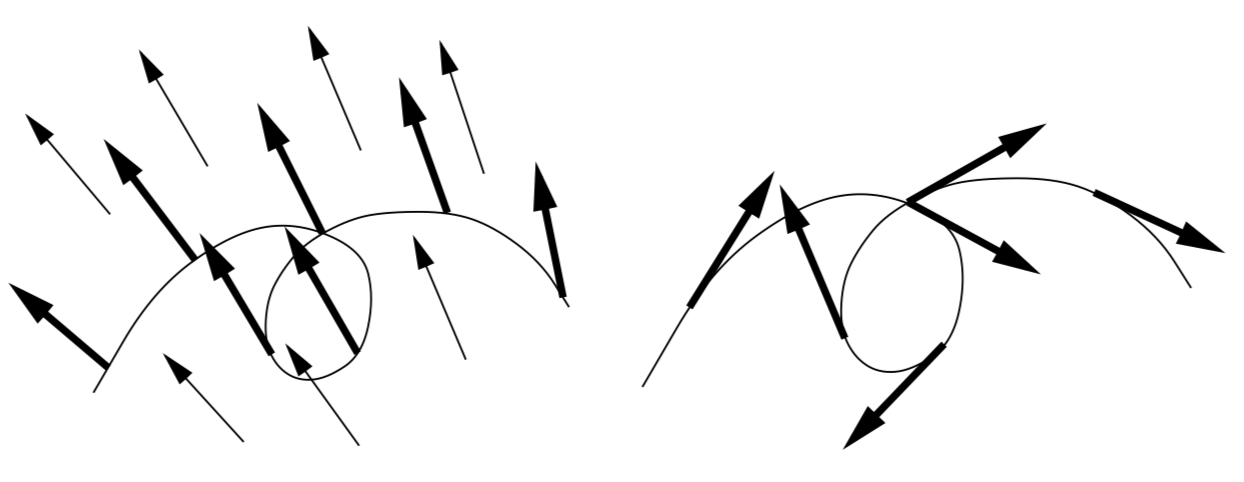
\includegraphics[width=0.5\textwidth]{Figs/3.png}
    \caption{Extendible and nonextendible vector}
    \label{fig:trgfdsf}
\end{figure}
\end{defa}
\begin{rema}
Note, however, locally we can always extend the curve to a vector field. This is no uniqueness here however. There may exist different vector fields that coincide along the curve.
\end{rema}


Now we can address the question that originally motivated the definition of connections: How can we make sense of the directional derivative of a vector field along a curve? \tb{We use the notion of ``extendible'' to get the directional derivative of a vector field along a curve from the surrounding extended vector field.} \cref{lem:oindfae} is then applicable.).
\begin{lema}
Let $\nabla$ be a linear connection on $M$. For each curve $\gamma: I \rightarrow$ $M, \nabla$ determines a unique operator
\begin{align*}
D_{t}: \mathcal{T}(\gamma) \rightarrow \mathcal{T}(\gamma)
\end{align*}
satisfying the following properties:
\begin{enumerate}
    \item Linearity over $\mathbf{R}$ :
\begin{align*}
D_{t}(a V+b W)=a D_{t} V+b D_{t} W \quad \text { for } a, b \in \mathbf{R} .
\end{align*}
\item Product rule:
\begin{align*}
D_{t}(f V)=\dot{f} V+f D_{t} V \quad \text { for } f \in C^{\infty}(I) .
\end{align*}
\item If $V$ is extendible, then for any extension $\tilde{V}$ of $V$,
\begin{align*}
D_{t} V(t)=\nabla_{\dot{\gamma}(t)} \tilde{V} .
\end{align*}
\end{enumerate}
For any $V \in \mathcal{T}(\gamma), D_{t} V$ is called the covariant derivative of $V$ along $\gamma$.
\end{lema} 
\begin{rema}\bfs{notation}
 Sometimes  we also write $D_t\dot{\gamma}(t) $ as $ \nabla_{v_{\gamma}}v_{\gamma} $ or $ \nabla_{\dot{\gamma}(t)}\dot{\gamma}(t) $
\end{rema}
\begin{proof}
First we show uniqueness. Suppose $D_{t}$ is such an operator, and let $t_{0} \in I$ be arbitrary. An argument similar to that of \cref{lem:ondfad} shows that the value of $D_{t} V$ at $t_{0}$ depends only on the values of $V$ in any interval $\left(t_{0}-\varepsilon, t_{0}+\varepsilon\right)$ containing $t_{0}$. (If $I$ has an endpoint, extend $\gamma$ to a slightly bigger open interval, prove the lemma there, and then restrict back to $I$.) Choose coordinates near $\gamma\left(t_{0}\right)$, and write
\begin{align*}
V(t)=V^{j}(t) \partial_{j}
\end{align*}
near $t_{0}$. Then by the properties of $D_{t}$, since $\partial_{j}$ is extendible,
\begin{align}
\begin{aligned}
D_{t} V\left(t_{0}\right) &=\dot{V}^{j}\left(t_{0}\right) \partial_{j}+V^{j}\left(t_{0}\right) \nabla_{\dot{\gamma}\left(t_{0}\right)} \partial_{j} \\
&=\left(\dot{V}^{k}\left(t_{0}\right)+V^{j}\left(t_{0}\right) \dot{\gamma}^{i}\left(t_{0}\right) \Gamma_{i j}^{k}\left(\gamma\left(t_{0}\right)\right)\right) \partial_{k} .\label{eq:oindfadf}
\end{aligned}
\end{align}
This shows that such an operator is unique if it exists.
For existence, if $\gamma(I)$ is contained in a single chart, we can define $D_{t} V$ by \cref{eq:oindfadf}; the easy verification that it satisfies the requisite properties is left to the reader. In the general case, we can cover $\gamma(I)$ with coordinate charts and define $D_{t} V$ by this formula in each chart, and uniqueness implies the various definitions agree whenever two or more charts overlap.
\end{proof}
\section{Parallel Transport and Curvature}
$\bullet$ \tb{Motivation:}

Image that you move with your nose (a tangent vector at each point) forward (no change of the direction). If you are on a \tb{flat} surface your nose will be pointing in exactly the same direction as it was at the start. If you were on a \tb{curved} surface, it is possible that your nose is now pointing in a different direction.
\begin{center}
    \btik
        \draw[thick, fill = gray!40, opacity = 0.4] (-10,-1.5) -- (-10,1.5) -- (-5,1.5) -- (-5,-1.5) -- (-10,-1.5);
        \draw[thick] (-10,-1.5) -- (-10,1.5) -- (-5,1.5) -- (-5,-1.5) -- (-10,-1.5);
        \draw[blue, thick] (-9,1) .. controls (-10,-1) and (-8,-1) .. (-6.5,-0.5) .. controls (-5.5,0.5) and (-8.5,1.5) .. (-9,1);
        %
        \draw[ultra thick, red, ->] (-9,1) -- (-9,0.5);
        \draw[ultra thick, red, ->] (-9.27,0) -- (-9.27,-0.5);
        \draw[ultra thick, red, ->] (-8.5,-0.7) -- (-8.5,-1.2);
        \draw[ultra thick, red, ->] (-7.5,-0.7) -- (-7.5,-1.2);
        \draw[ultra thick, red, ->] (-6.5,-0.5) -- (-6.5,-1);
        \draw[ultra thick, red, ->] (-7,0.75) -- (-7,0.25);
        \draw[ultra thick, red, ->] (-8,1.1) -- (-8,0.6);
        %%
        \shade[ball color = gray!40, opacity = 0.4] (0,0) circle (2cm);
        \draw[thick] (0,0) circle (2cm);
        \draw (-2,0) arc (180:360:2 and 0.6);
        \draw[dashed] (2,0) arc (0:180:2 and 0.6);
        %
        \draw[blue, thick, rotate around={90:(0,0)}] (2,0) arc (0:110:2 and 1);
        \draw[blue, thick,  rotate around={90:(0,0)}] (2,0) arc (0:103:2 and -1.5);
        %
        \node[circle, fill=black, inner sep=0.8pt] at (0,2) {};
        \node[circle, fill=black, inner sep=0.8pt] at (0,-2) {};
        %
        \draw[->, ultra thick, red] (0,2) -- (-1,2);
        \draw[->, ultra thick, red, xshift =-0.68cm, yshift = -0.5cm, rotate around={65:(0,2)}] (0,2) -- (-1,2);
        \draw[->, ultra thick, red, xshift =-1cm, yshift = -1.6cm, rotate around={85:(0,2)}] (0,2) -- (-1,2);
        \draw[->, ultra thick, red, xshift =-0.95cm, yshift = -2.5cm, rotate around={90:(0,2)}] (0,2) -- (-1,2);
        \draw[->, ultra thick, red, xshift =-0.4cm, yshift = -2.6cm, rotate around={90:(0,2)}] (0,2) -- (-1,2);
        \draw[->, ultra thick, red, xshift = 0.3cm, yshift = -2.6cm, rotate around={90:(0,2)}] (0,2) -- (-1,2);
        \draw[->, ultra thick, red, xshift = 0.9cm, yshift = -2.54cm, rotate around={90:(0,2)}] (0,2) -- (-1,2);
        \draw[->, ultra thick, red, xshift = 1.47cm, yshift = -2.4cm, rotate around={90:(0,2)}] (0,2) -- (-1,2);
        \draw[->, ultra thick, red, xshift = 1.47cm, yshift = -1.5cm, rotate around={100:(0,2)}] (0,2) -- (-1,2);
        \draw[->, ultra thick, red, xshift = 1.15cm, yshift = -0.7cm, rotate around={125:(0,2)}] (0,2) -- (-1,2);
        \draw[->, ultra thick, red, xshift = 0.5cm, yshift = -0.1cm, rotate around={150:(0,2)}] (0,2) -- (-1,2);
    \etik
\end{center}

Mathematically, what we are talking about is the directional derivative of a vector field. On the plane the vector field does not change no matter what path you take, and so the instructions of how to walk about are simply
\begin{align*}
    \nabla_{v_{\gamma}}X = 0
\end{align*}
where $\gamma$ is the path you take and $X$ is the vector field made by your arms. 

The instructions on the sphere are the same, but the result is different. This gives us our first hint that the \tb{covariant derivative somehow encodes the (intrinsic) curvature of the surface.} From here we can convince ourselves that the connection is what gives our manifold `shape'. That is both the sphere and the potato have $(S^2,\cO,\cA)$ as topological manifolds but they have different curvature and so have different connections, $\nabla_{\text{sphere}}$ and $\nabla_{\text{potato}}$. The aim of this section is to make this more precise. 

\subsection{Parallelity of Vector Fields}
In this section we shall assume that a connection has already been chosen for our manifold and so we are dealing with a smooth manifold $(\cM,\cO,\cA,\nabla)$.
\bd\bfs{Parallely Transported}\label{def:dfadfr}
    A vector field $X$ along a smooth curve $\gamma:\R\to\cM$ on $\cM$ is said to be \textbf{parallely transported along the curve} if 
    \begin{align*}
        \nabla_{v_{\gamma}}X = 0.
    \end{align*}
\ed 
We also have a slightly weaker condition.
\bd\bfs{Parallel I}
    A vector field $X$ in $\cM$ is said to be \textbf{parallel along a curve} $\gamma:\R\to\cM$ if
    \begin{align*}
        \nabla_{v_{\gamma}}X = \mu \cdot X,
    \end{align*}
    for $\mu:\R\to\R$ a smooth function. Written pointwise, that is
    \begin{align*}
        \big(\nabla_{v_{\gamma,\gamma(\lambda)}}X\big)_{\gamma(\lambda)} = \mu(\lambda) \cdot X_{\gamma(\lambda)}.
    \end{align*}
\ed 
\bd\bfs{Parallel Vector Field}\label{def:dincda}
    A vector field $X$ in $\cM$ is said to be \textbf{parallel}  if it is \textbf{parallely transported along all smooth curves}, namely for \tb{all} smooth $\gamma:\R\to\cM$
    \begin{align*}
        \nabla_{v_{\gamma}}X_{\gamma(t)} = 0
    \end{align*}
\ed 

% Note any parallely transported vector field is parallel -- simply choose $\mu(\lambda)=0$ for all $\lambda$.
\begin{rema}
Please note in \cref{def:dfadfr} the vector field is only defined over the curve which may not be extendible, while  in \cref{def:dincda}, we require the vector field to be defined  on the full domain $\cM$.
\end{rema}

\bex 
    Let our smooth affine manifold be the Euclidean plane $(\R^2,\cO,\cA,\nabla_E)$. The left drawing below is a parallely transported vector field, the middle drawing is a parallel vector field and the right drawing is not even parallel.
    \begin{center}
        \btik
            \draw[thick, blue] (-4,0) .. controls (-5,1.2) and (0,1.5) .. (-1,3);
            \draw[thick, blue] (0,0) .. controls (-1,1.2) and (4,1.5) .. (3,3);
            \draw[thick, blue] (5,0) .. controls (4,1.2) and (9,1.5) .. (8,3);
            %
            \draw[->, thick, rotate around={45: (-4,0)}] (-4,0) -- (-4,1);
            \draw[->, thick, rotate around={45: (-3.5,0.95)}] (-3.5,0.95) -- (-3.5,1.95);
            \draw[->, thick, rotate around={45:(-2.5,1.38)}] (-2.5,1.38) -- (-2.5,2.38);
            \draw[->, thick, rotate around={45:(-1.5,1.85)}] (-1.5,1.85) -- (-1.5,2.85);
            \draw[->, thick, rotate around={45:(-0.9,2.4)}] (-0.9,2.4) -- (-0.9,3.4);
            %
            \draw[->, thick, rotate around={45: (0,0)}] (0,0) -- (0,1.5);
            \draw[->, thick, rotate around={45: (0.5,0.95)}] (0.5,0.95) -- (0.5,1.55);
            \draw[->, thick, rotate around={45:(1.5,1.38)}] (1.5,1.38) -- (1.5,0.38);
            \draw[->, thick, rotate around={45:(2.5,1.85)}] (2.5,1.85) -- (2.5,2.5);
            \draw[->, thick, rotate around={45:(3.1,2.4)}] (3.1,2.4) -- (3.1,4.4);
            % 
            \draw[->, thick, rotate around={50: (5,0)}] (5,0) -- (5,1);
            \draw[->, thick, rotate around={-25: (5.5,0.95)}] (5.5,0.95) -- (5.5,1.5);
            \draw[->, thick] (6.5,1.38) -- (6.5,0.2);
            \draw[->, thick, rotate around={60:(7.5,1.85)}] (7.5,1.85) -- (7.5,3);
            \draw[->, thick, rotate around={-45:(8.1,2.4)}] (8.1,2.4) -- (8.1,3.4);
        \etik
    \end{center}
    In the middle drawing it is important that the vector field vanishes in-between the points when it points `up' vs. `down', as $\mu:\R\to\R$ is smooth.
\eex 

The fundamental fact about parallel vector fields is that any tangent vector at any point on a curve can be uniquely extended to a parallel vector field along the entire curve.

\begin{thma}\bfs{Parallel Translation}
  Given a curve $\gamma: I \rightarrow M, t_{0} \in$ $I$, and a vector $V_{0} \in T_{\gamma\left(t_{0}\right)} M$, there exists a unique parallel vector field $V$ along $\gamma$ such that $V\left(t_{0}\right)=V_{0}$.
\end{thma}
\begin{proof}
    Similar to the proof of \cref{lem:dfafdaf}, it is because linear ODE solution exists and is unique.
\end{proof}
\begin{defa}
If $\gamma: I \rightarrow M$ is a curve and $t_{0}, t_{1} \in I$, parallel translation defines an operator
\begin{align*}
P_{t_{0} t_{1}}: T_{\gamma\left(t_{0}\right)} M \rightarrow T_{\gamma\left(t_{1}\right)} M
\end{align*}
 by setting $P_{t_{0} t_{1}} V_{0}=V\left(t_{1}\right)$, where $V$ is the parallel translate of $V_{0}$ along $\gamma$. 
\end{defa}

 \begin{lema}
   It is easy to check that this is a linear isomorphism between $T_{\gamma\left(t_{0}\right)} M$ and $T_{\gamma\left(t_{1}\right)} M$ (because the equation of parallelism is linear). 
 \end{lema}
 The next lemma shows that covariant differentiation along $\gamma$ can be recovered from this operator. This is the sense in which a connection "connects" nearby tangent spaces.
\begin{lema}
Let $\nabla$ be a linear connection on $M$. Show that covariant differentiation along a curve $\gamma$ can be recovered from parallel translation, by the following formula:
\begin{align*}
D_{t} V\left(t_{0}\right)=\lim _{t \rightarrow t_{0}} \frac{P_{t_{0} t}^{-1} V(t)-V\left(t_{0}\right)}{t-t_{0}}
\end{align*}
[Hint: Use a parallel frame along $\gamma$.]
\end{lema}
 
 
\subsection{Autoparallelly Transported Curves}
As the name suggests, an \textit{auto}parallely transported curve is one that is parallely transported along itself. What we mean by this is to take the starting point of the curve and look at its tangent vector and then tell the curve to follow that direction. You then repeat this for every point along the curve. It is the idea of `follow where your nose is pointing' experiment. 

\begin{rema}\bfs{straightest curve}
 This gives us a great intuitive insight: we are travelling along the \tb{straightest} curve between two points. Note we say straightest and not shortest, as we still don't have a notion of length yet. Note also that the straightest line might not actually look straight when `viewed from above'. That is, if we embed the manifold into a higher dimensional one and then look just at the curve, it might look curved. For example, on the sphere a straight line traces out a portion of a circle around the sphere. This does not look straight in the (Euclidean) embedding, however \tb{on the surface} it is the straightest line.
\end{rema}
\bd\bfs{Autoparallely Transported}
    A smooth curve $\gamma:\R\to\cM$ is called \textbf{autoparallely transported} if 
    \begin{align*}
        \nabla_{v_{\gamma}}v_{\gamma} = 0.
    \end{align*}
\ed 

\bd 
    A smooth curve $\gamma:\R\to\cM$ is called an \textbf{autoparallel} if
    \begin{align*}
        \nabla_{v_{\gamma}}v_{\gamma} = \mu\cdot v_{\gamma}.
    \end{align*}
\ed

\bex 
    Again consider the Euclidean plane $(\R^2,\cO,\cA,\nabla_E)$. If we represent equal parameter changes by dashes in our drawings we have the following drawings, where the left is a autoparallely transported curve and the right is just a autoparallel.
    \begin{center}
        \btik 
            \draw[thick] (-2,-2) -- (-1.5,-1.5);
            \draw[thick] (-1.4,-1.4) -- (-0.9,-0.9);
            \draw[thick] (-0.8,-0.8) -- (-0.3,-0.3);
            \draw[thick] (-0.2,-0.2) -- (0.3,0.3);
            \draw[thick] (0.4,0.4) -- (0.9,0.9);
            \draw[thick] (1,1) -- (1.5,1.5);
            %
            \draw[thick] (2,-2) -- (2.5,-1.5);
            \draw[thick] (2.6,-1.4) -- (3,-1);
            \draw[thick] (3.1,-0.9) -- (3.3,-0.7);
            \draw[thick] (3.4,-0.6) -- (3.5,-0.5);
            \draw[thick] (3.6,-0.4) -- (3.8,-0.2);
            \draw[thick] (3.9,-0.1) -- (4.3,0.3);
            \draw[thick] (4.4,0.4) -- (4.9,0.9);
            \draw[thick] (5,1) -- (5.5,1.5);
        \etik 
    \end{center}
\eex 

\bter 
    People also refer to autoparallely transported vector fields as simply \textit{autoparallels}. We follows this convection and when we mention \textit{autoparallels}, we mean \textit{autoparallely transported.}
\eter 
\begin{thma}\bfs{Existence and Uniqueness of Autoparallel}\label{lem:dfafdaf}
Let $M$ be a manifold with a linear connection. For any $p \in M$, any $V \in T_{p} M$, and any $t_{0} \in \mathbf{R}$, there exist an open interval $I \subset \mathbf{R}$ containing $t_{0}$ and a geodesic $\gamma: I \rightarrow M$ satisfying $\gamma\left(t_{0}\right)=p, \dot{\gamma}\left(t_{0}\right)=V$. Any two such geodesics agree on their common domain.
\end{thma}
\begin{proof}
    It comes from the linear ODE solution exists and is unique. See out notes where the smooth has indicated Lipschitz continuous. 
\end{proof}
\subsection{Autoparallel Equation}

Consider an autoparallel $\gamma:\R\to\cM$ and consider the portion of the curve that lies in $U\se \cM$ where $(U,x)\in\cA$. We would like to express the condition $\nabla_{v_{\gamma}}v_{\gamma}=0$ in terms of chart representatives of the objects. From  \cref{eq:oindfadf}. we get \tb{autoparallel equation} (notation slight different, but as you know, local frame is just the $\Gamma$s over one chart.)
\begin{align*}
    \Ddot{\gamma}^i_{(x)}(\lambda) + \Gamma^i_{(x)jk}\big|_{\gamma(\lambda)}\Dot{\gamma}^k_{(x)}(\lambda)\Dot{\gamma}^j_{(x)}(\lambda) = 0,
\end{align*}
which is the chart expression that the curve $\gamma$ be autoparallely transported.

\br
\label{rem:Acc}\bfs{what is acceleration?}
    We know that the complete autoparallel equation transforms like a vector (as it comes from $\nabla_{v_{\gamma}}v_{\gamma}$, which is a vector). However we have already seen that the $\Gamma$s are not tensors and so do not transform nicely. We see, then, the \tb{$\Ddot{\gamma}$ must also not be a tensor itself,} but must transform in such a way as to cancel the bad parts from the $\Gamma$s. 
    
    This is an important fact to note, as one is often tempted to call $\Ddot{\gamma}$ the \textit{acceleration} along $\gamma$, but it is not (as acceleration is a vector). In fact the \tb{acceleration is the complete autoparallel equation}. This is actually a very nice result as it tells us that the condition for \tb{a straight line is that the acceleration along the line vanishes}! It is only in a flat space, in a chart where we take the $\Gamma$s to all vanish that we recover $a=\Ddot{\gamma}$.
\er 

\bd\bfs{Acceleration}
    Let $\gamma:\R\to\cM$ be a smooth curve on an affine manifold $(\cM,\cO,\cA,\nabla)$, and let $v_{\gamma}$ be the velocity field along $\gamma$. Then the \textbf{acceleration} field along $\gamma$ is given by 
    \begin{align*}
        a_{\gamma} := \nabla_{v_{\gamma}} v_{\gamma}.
    \end{align*}
\ed 

\bex 
    Consider the Euclidean plane $(\R^2,\cO,\cA,\nabla_E)$ and the chart $(U,x) = (\R^2,Id_{\R^2})$ so that $\Gamma^i_{(x)jk}=0$ for all $i,j,k=1,2$. Then our autoparallel equation simply reads 
    \begin{align*}
        \Ddot{\gamma}^i_{(x)}(\lambda) = 0 \quad \implies \quad \gamma^i_{(x)}(\lambda) = a^i\lambda + b^i,
    \end{align*}
    where $a^i,b^i\in\R$. This is just what we normally think of as the equation for a straight line. Note, however, this is only valid in this chart. If we transformed to polar coordinates the $\Gamma$s wouldn't vanish and so the expression for $\gamma$ would be different.
\eex 

\bex 
    Now consider the so-called round sphere $(S^2,\cO,\cA,\nabla_{\text{round}})$ and the chart $(U,x)$ with $x(p) = (\theta,\varphi)$, where $\theta \in (0,\pi)$ and $\varphi\in(0,2\pi)$, which are the usual spherical coordinates.
    
    We define $\nabla_{\text{round}}$ to be such that 
    \begin{align*}
        \Gamma^1_{(x)22}\big|_{x^{-1}(\theta,\varphi)} = - \sin\theta \cos\theta, \qquad \Gamma^2_{(x)12}\big|_{x^{-1}(\theta,\varphi)} = \Gamma^2_{(x)21}\big|_{x^{-1}(\theta,\varphi)} = \cot\theta,
    \end{align*}
    and all other $\Gamma$s vanishing. If we now introduce the (sloppy) notation 
    \begin{align*}
        x^1(p) = \theta(p), \qquad \text{and} \qquad x^2(p) = \varphi(p),
    \end{align*}
    then the autoparallel equation tells us 
    \begin{align*}
        \begin{split}
            \Ddot{\theta} + \Gamma^1_{(x)22} \Dot{\varphi}\Dot{\varphi} = \Ddot{\theta} -\sin(\theta)\cos(\theta) \Dot{\varphi}\Dot{\varphi} & = 0 \\
            \Ddot{\varphi} + 2\Gamma^2_{(x)12}\Dot{\varphi}\Dot{\theta} = \Ddot{\varphi} +2\cot(\theta)\Dot{\varphi}\Dot{\theta} & = 0.
        \end{split}
    \end{align*}
    Now look at solutions to these equations. One solution is 
    \begin{align*}
        \theta(\lambda) = \frac{\pi}{2} \qquad \text{and}\qquad \varphi(\lambda) = \omega \cdot \lambda + \varphi_0,
    \end{align*}
    for $\omega,\varphi_0\in\R$, which is checked by direct substitution. These equations correspond to just going around the equator of the sphere at a constant speed. 
    You can show that any curve that goes right round the sphere (e.g. North pole to South pole and back) will satisfy these equations. So we see that the straightest curves (that is the curves that satisfy the autoparallel equation) on the round sphere are just curves that go all the way around. This is why this choice of $\Gamma$s corresponds to the round sphere; we think of a round sphere as one whose straight lines behave like this.
\eex 
\subsection{Torsion}

Question: Can one use $\nabla$ to define tensors on $(\cM,\cO,\cA,\nabla)$? 

Answer: Yes. 

\bd[Torsion]
    The \textbf{torsion} of a connection $\nabla$ is the $(1,2)$-tensor field
    \begin{align*}
        T(\omega,X,Y) :=  \omega : \big(\nabla_XY - \nabla_YX - [X,Y]\big),
    \end{align*}
    where $[\cdot,\cdot]: \Gamma T\cM \times \Gamma T\cM \to \Gamma T\cM$ is the commutator\footnote{In fact turn this is a Lie bracket by restricting to $\R$-linearity instead of $C^{\infty}$-linearity, and define the Lie algebra of vector fields.} on $\Gamma T\cM$ given by 
    \begin{align*}
        [X,Y]\la f \ra := X\big\la Y\la f\ra \big\ra - Y\big\la X\la f\ra \big\ra.
    \end{align*}
\ed 
\begin{lema}
 $T_{i j}^{k}=\Gamma_{i j}^{k}-\Gamma_{j i}^{k}$
\end{lema}
\begin{proof}
    $$T^i_{ab}:= T(dx^i, \frac{\p}{\p^a}, \frac{\p}{\p^b})=dx^i(...)=\Gamma^i_{ab}-\Gamma^i_{ba}$$
\end{proof}
% \bbox 
%     Prove that $T$ is $C^{\infty}$ linear in each entry, which we require if $T$ is to be a tensor.
% \ebox 

\bd\bfs{Torsion Free Connection}
    A manifold $(\cM,\cO,\cA,\nabla)$ is called \textbf{torsion free} if the torsion tensor $T$ vanishes everywhere. One can also say that the connection is torsion free. This is often just written as 
    \begin{align*}
        \nabla_XY - \nabla_YX = [X,Y]
    \end{align*}
    for all $X,Y\in\Gamma T\cM$.
\ed 
$\bullet$ \tb{Explanation}
\begin{enumerate}
    \item  The Lie commutator $[\cdot,\cdot]$ tell us the difference between $X$ take derivative along $Y$ (view it as a curve) and $Y$ take derivative along $X$. Note it does not depends on the connection. However, we cannot define it at a specific point. This can be seen if you try to expand it using the local chart representation and note we will need to calculate $\partial_x f$ (which is well defined using a neighbour \href{https://math.stackexchange.com/questions/2705586/composition-of-vector-field-regarded-as-sections-of-tangent-bundle}{(See the link)}).
    See Lie Derivatives in \cref{sub:inbdarqr} for more details.
\begin{figure}[h]
     \centering
     \begin{subfigure}[b]{0.4\textwidth}
         \centering
         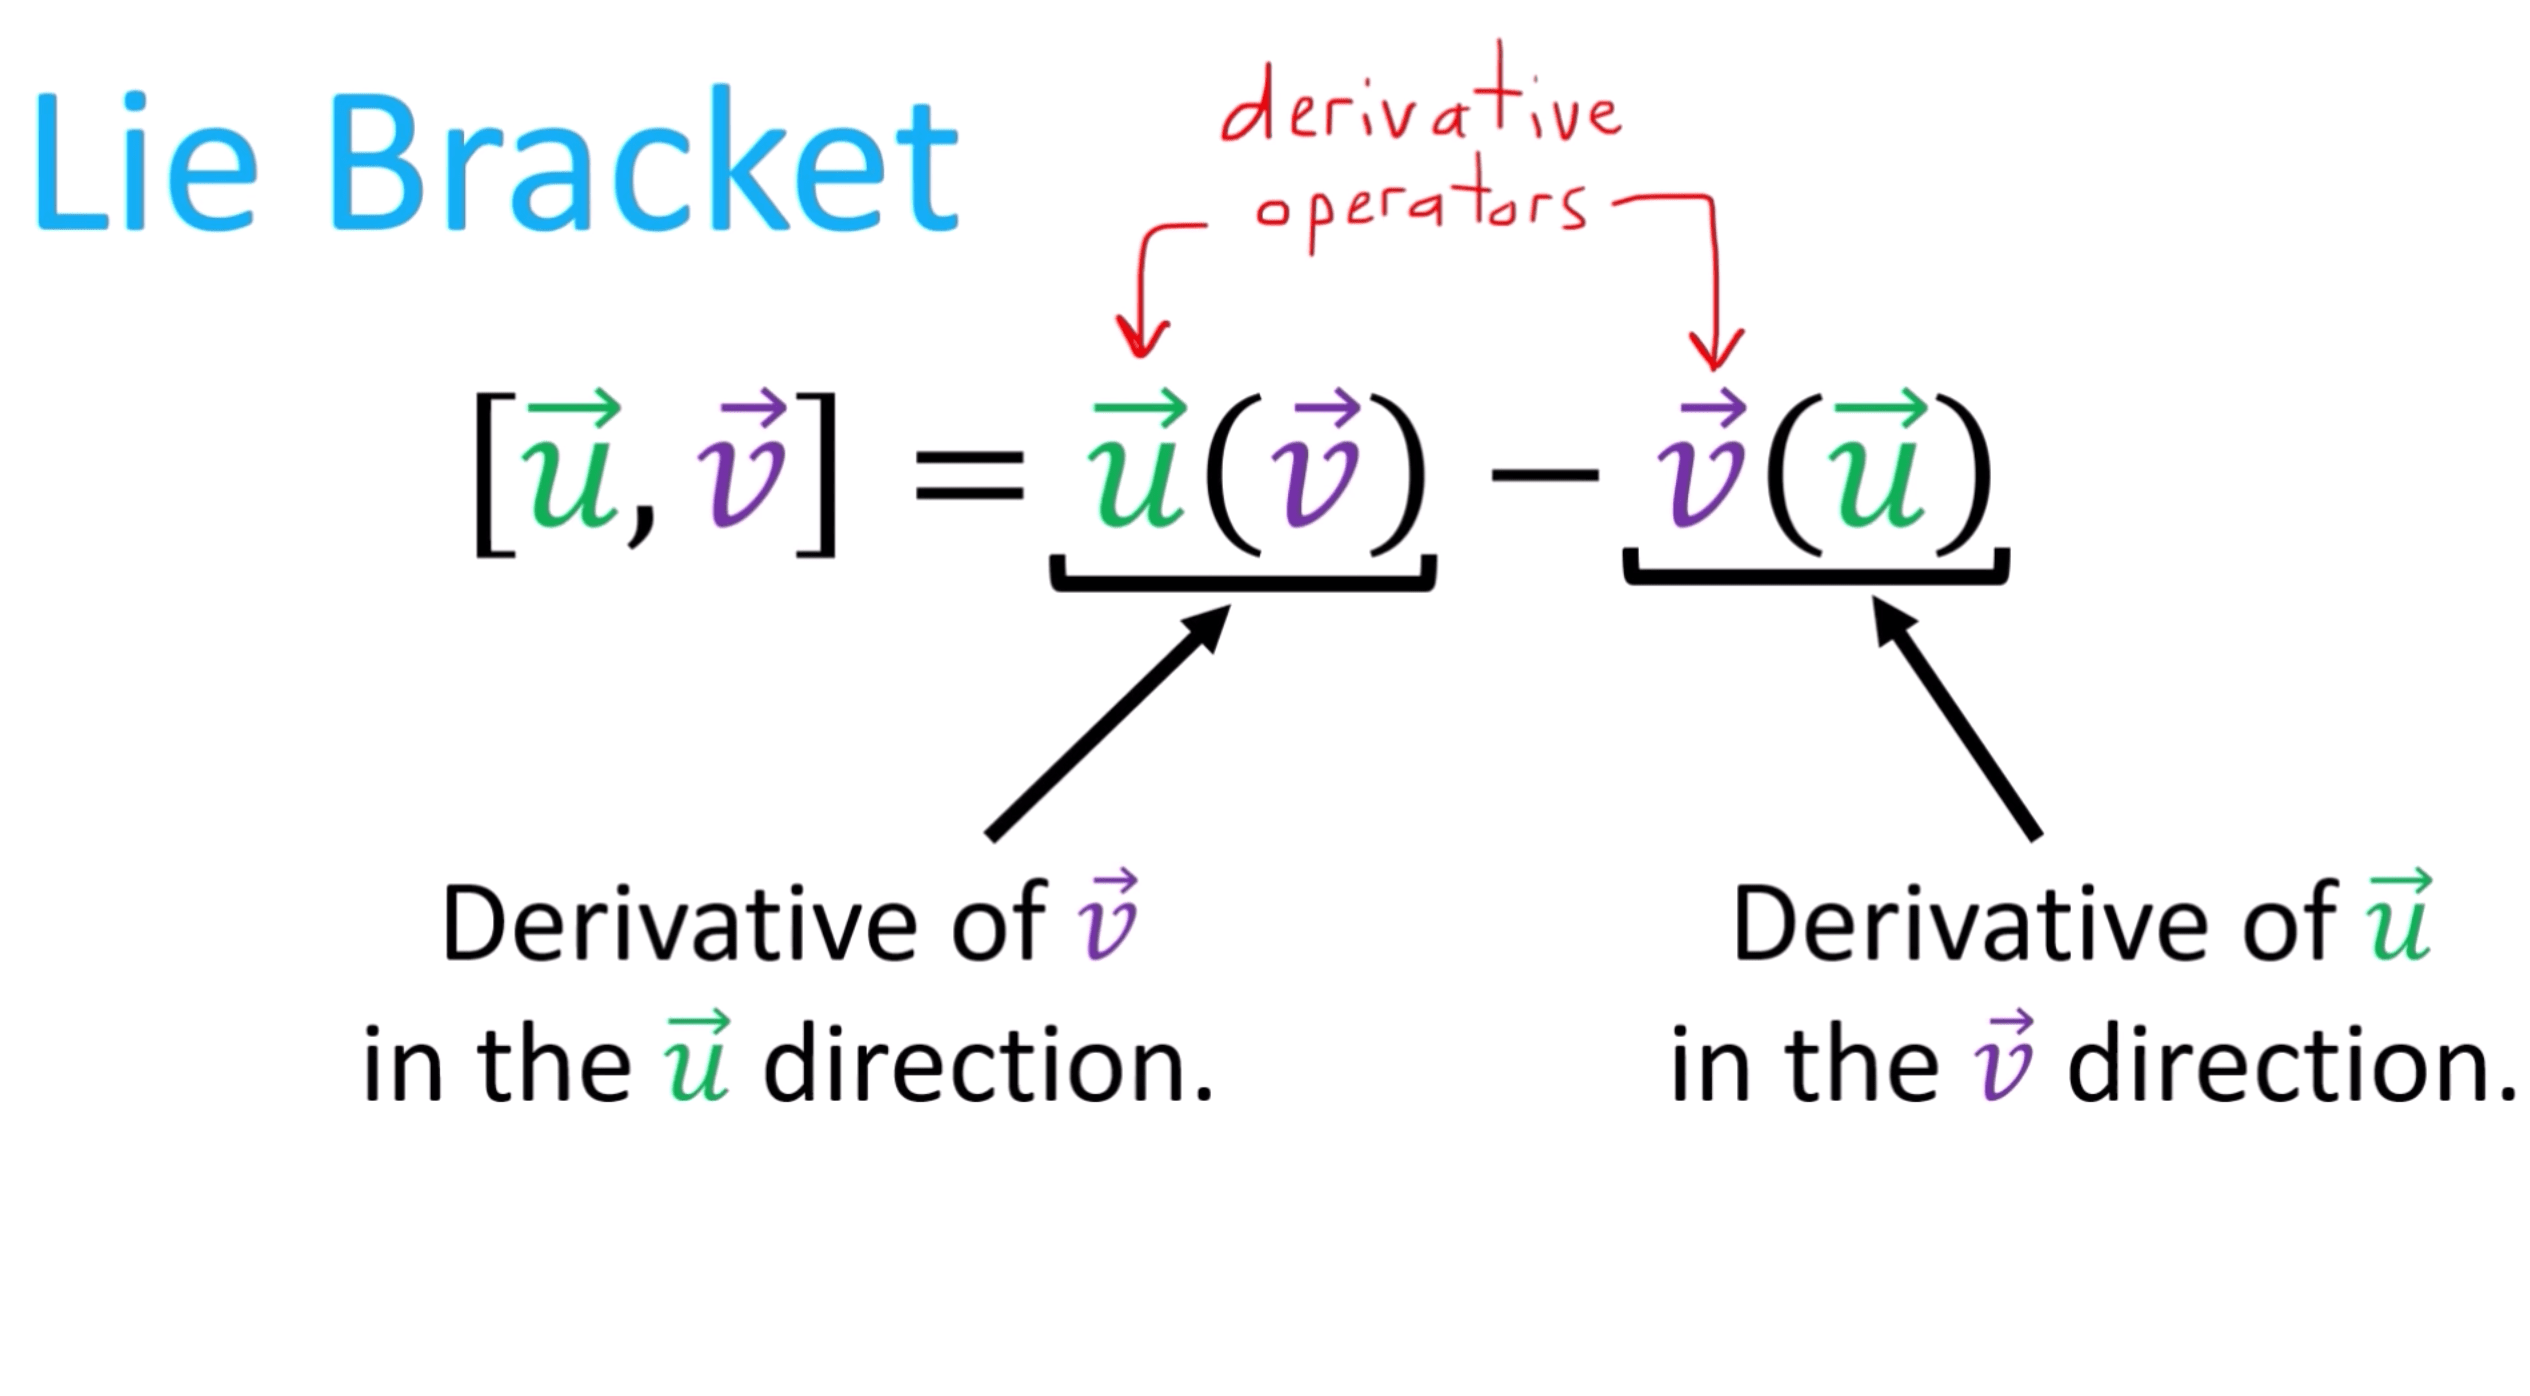
\includegraphics[width=\textwidth]{Figs/lie_bracket1-min.png}
     \end{subfigure}
     \hfill
     \begin{subfigure}[b]{0.4\textwidth}
         \centering
         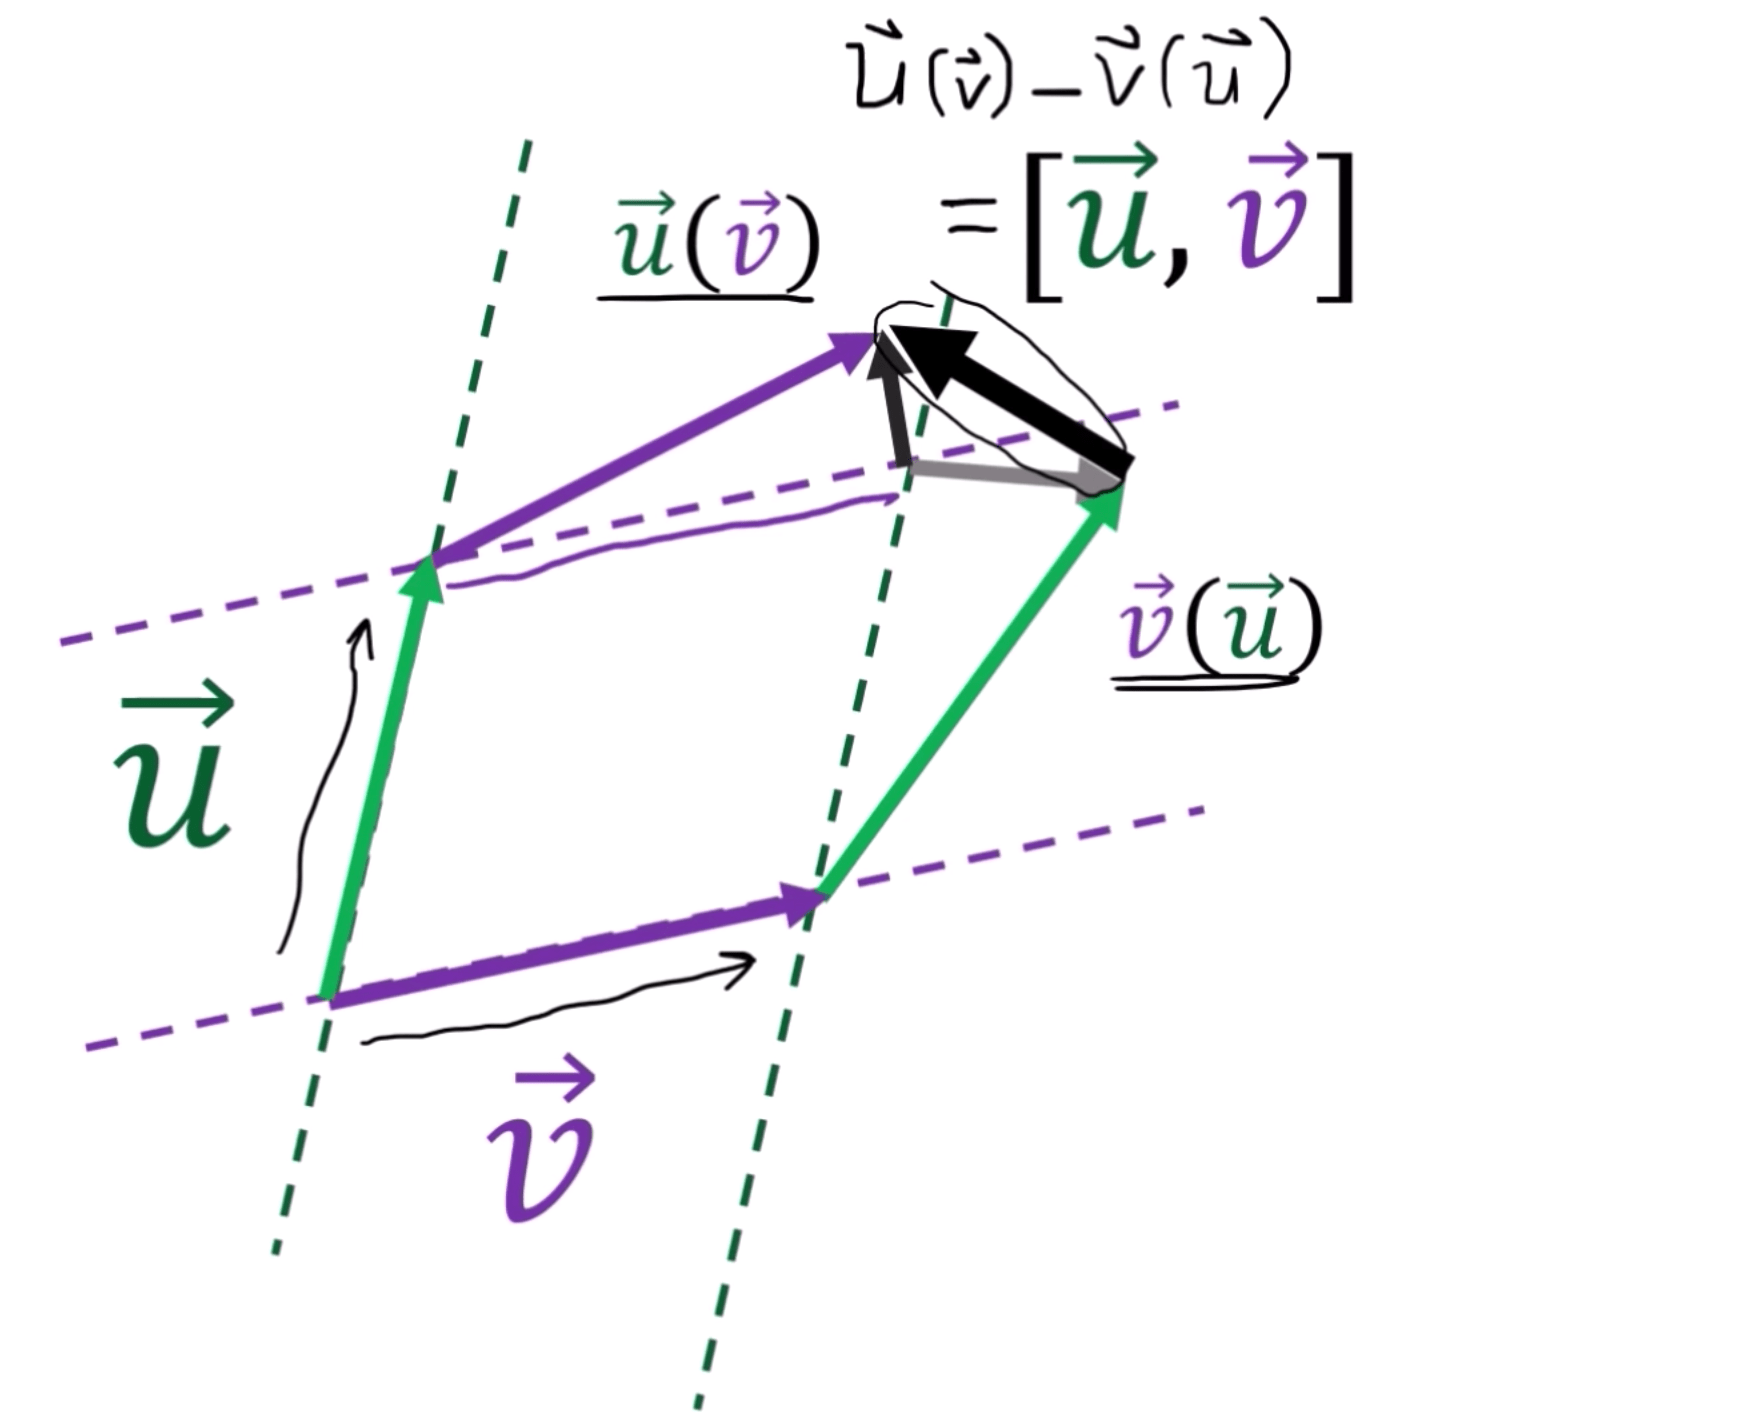
\includegraphics[width=\textwidth]{Figs/lie_bracket2-min.png}
     \end{subfigure}
\end{figure}
\item Here we just take into consideration $ \nabla_XY - \nabla_YX - [X,Y]$.  Note unlike the $ X\big\la Y\la f\ra \big\ra$, $\nabla_XY$ measures how much the difference of $Y$ at each point is away from the vector field by letting $Y_p$ to parallel transport among the $X$ direction.
\tb{Torsion free} means the parallel transported vectors close properly.
\begin{figure}[h]
     \centering
     \begin{subfigure}[b]{0.4\textwidth}
         \centering
         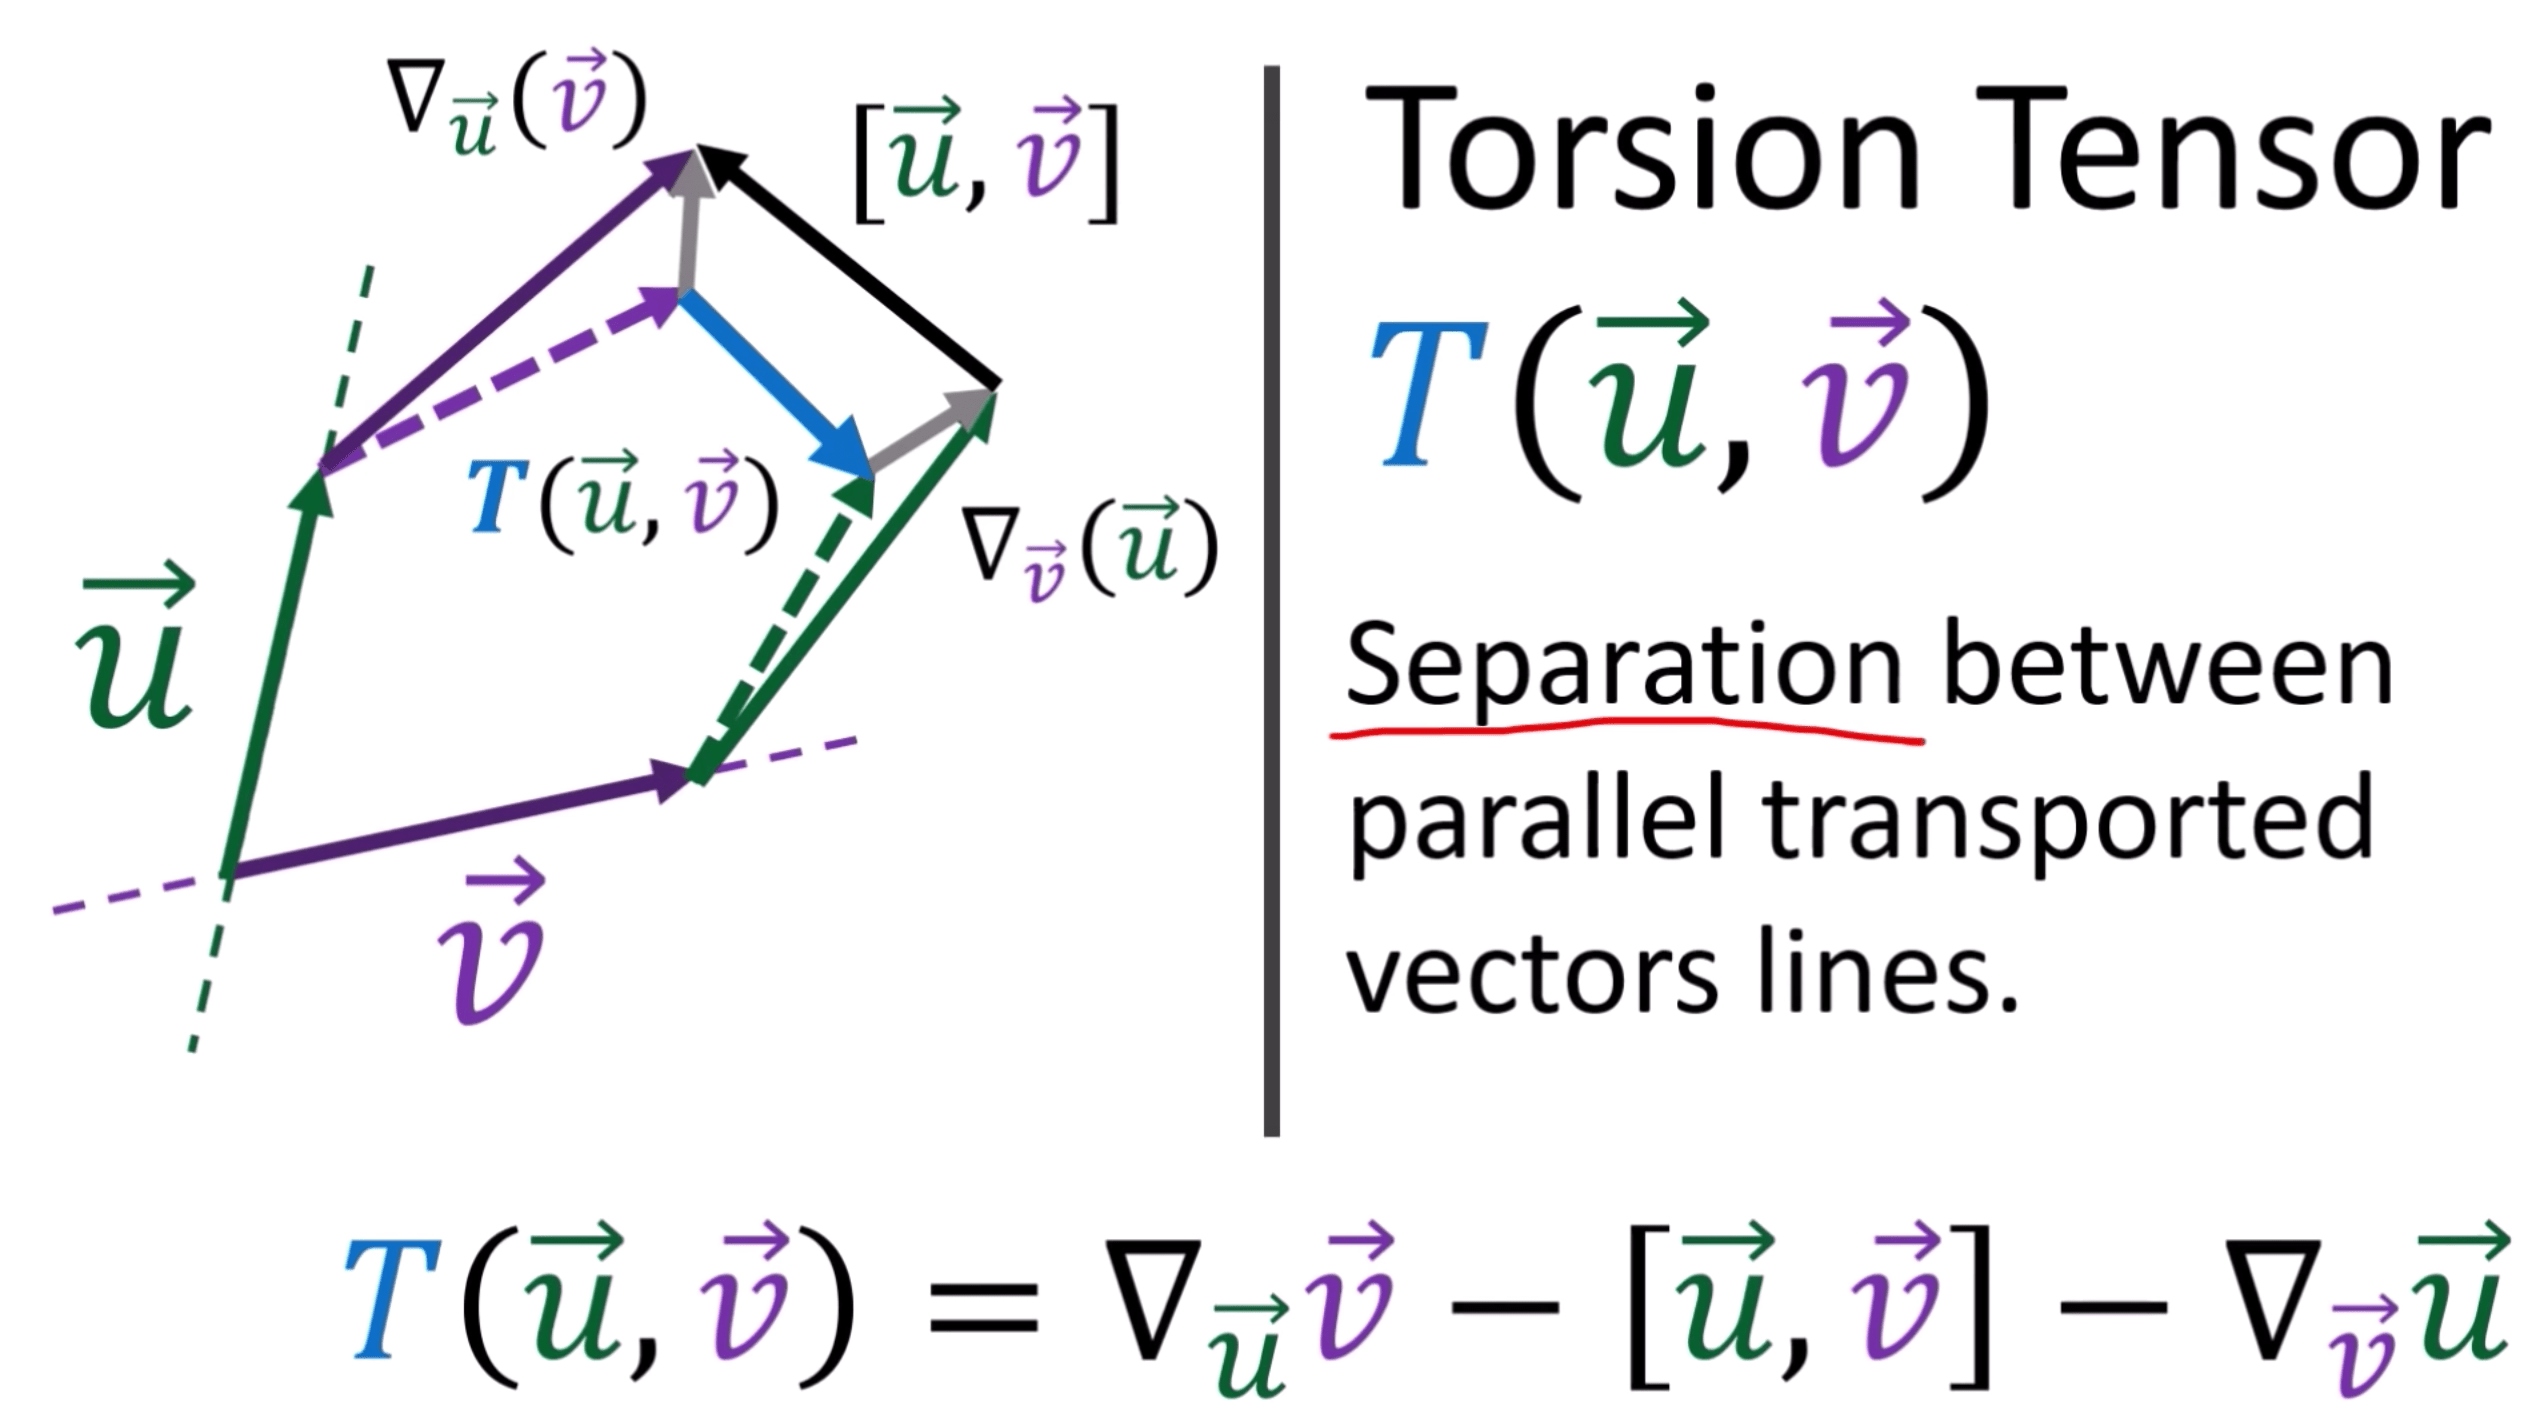
\includegraphics[width=\textwidth]{Figs/torsion1-min.png}
     \end{subfigure}
     \hfill
     \begin{subfigure}[b]{0.4\textwidth}
         \centering
         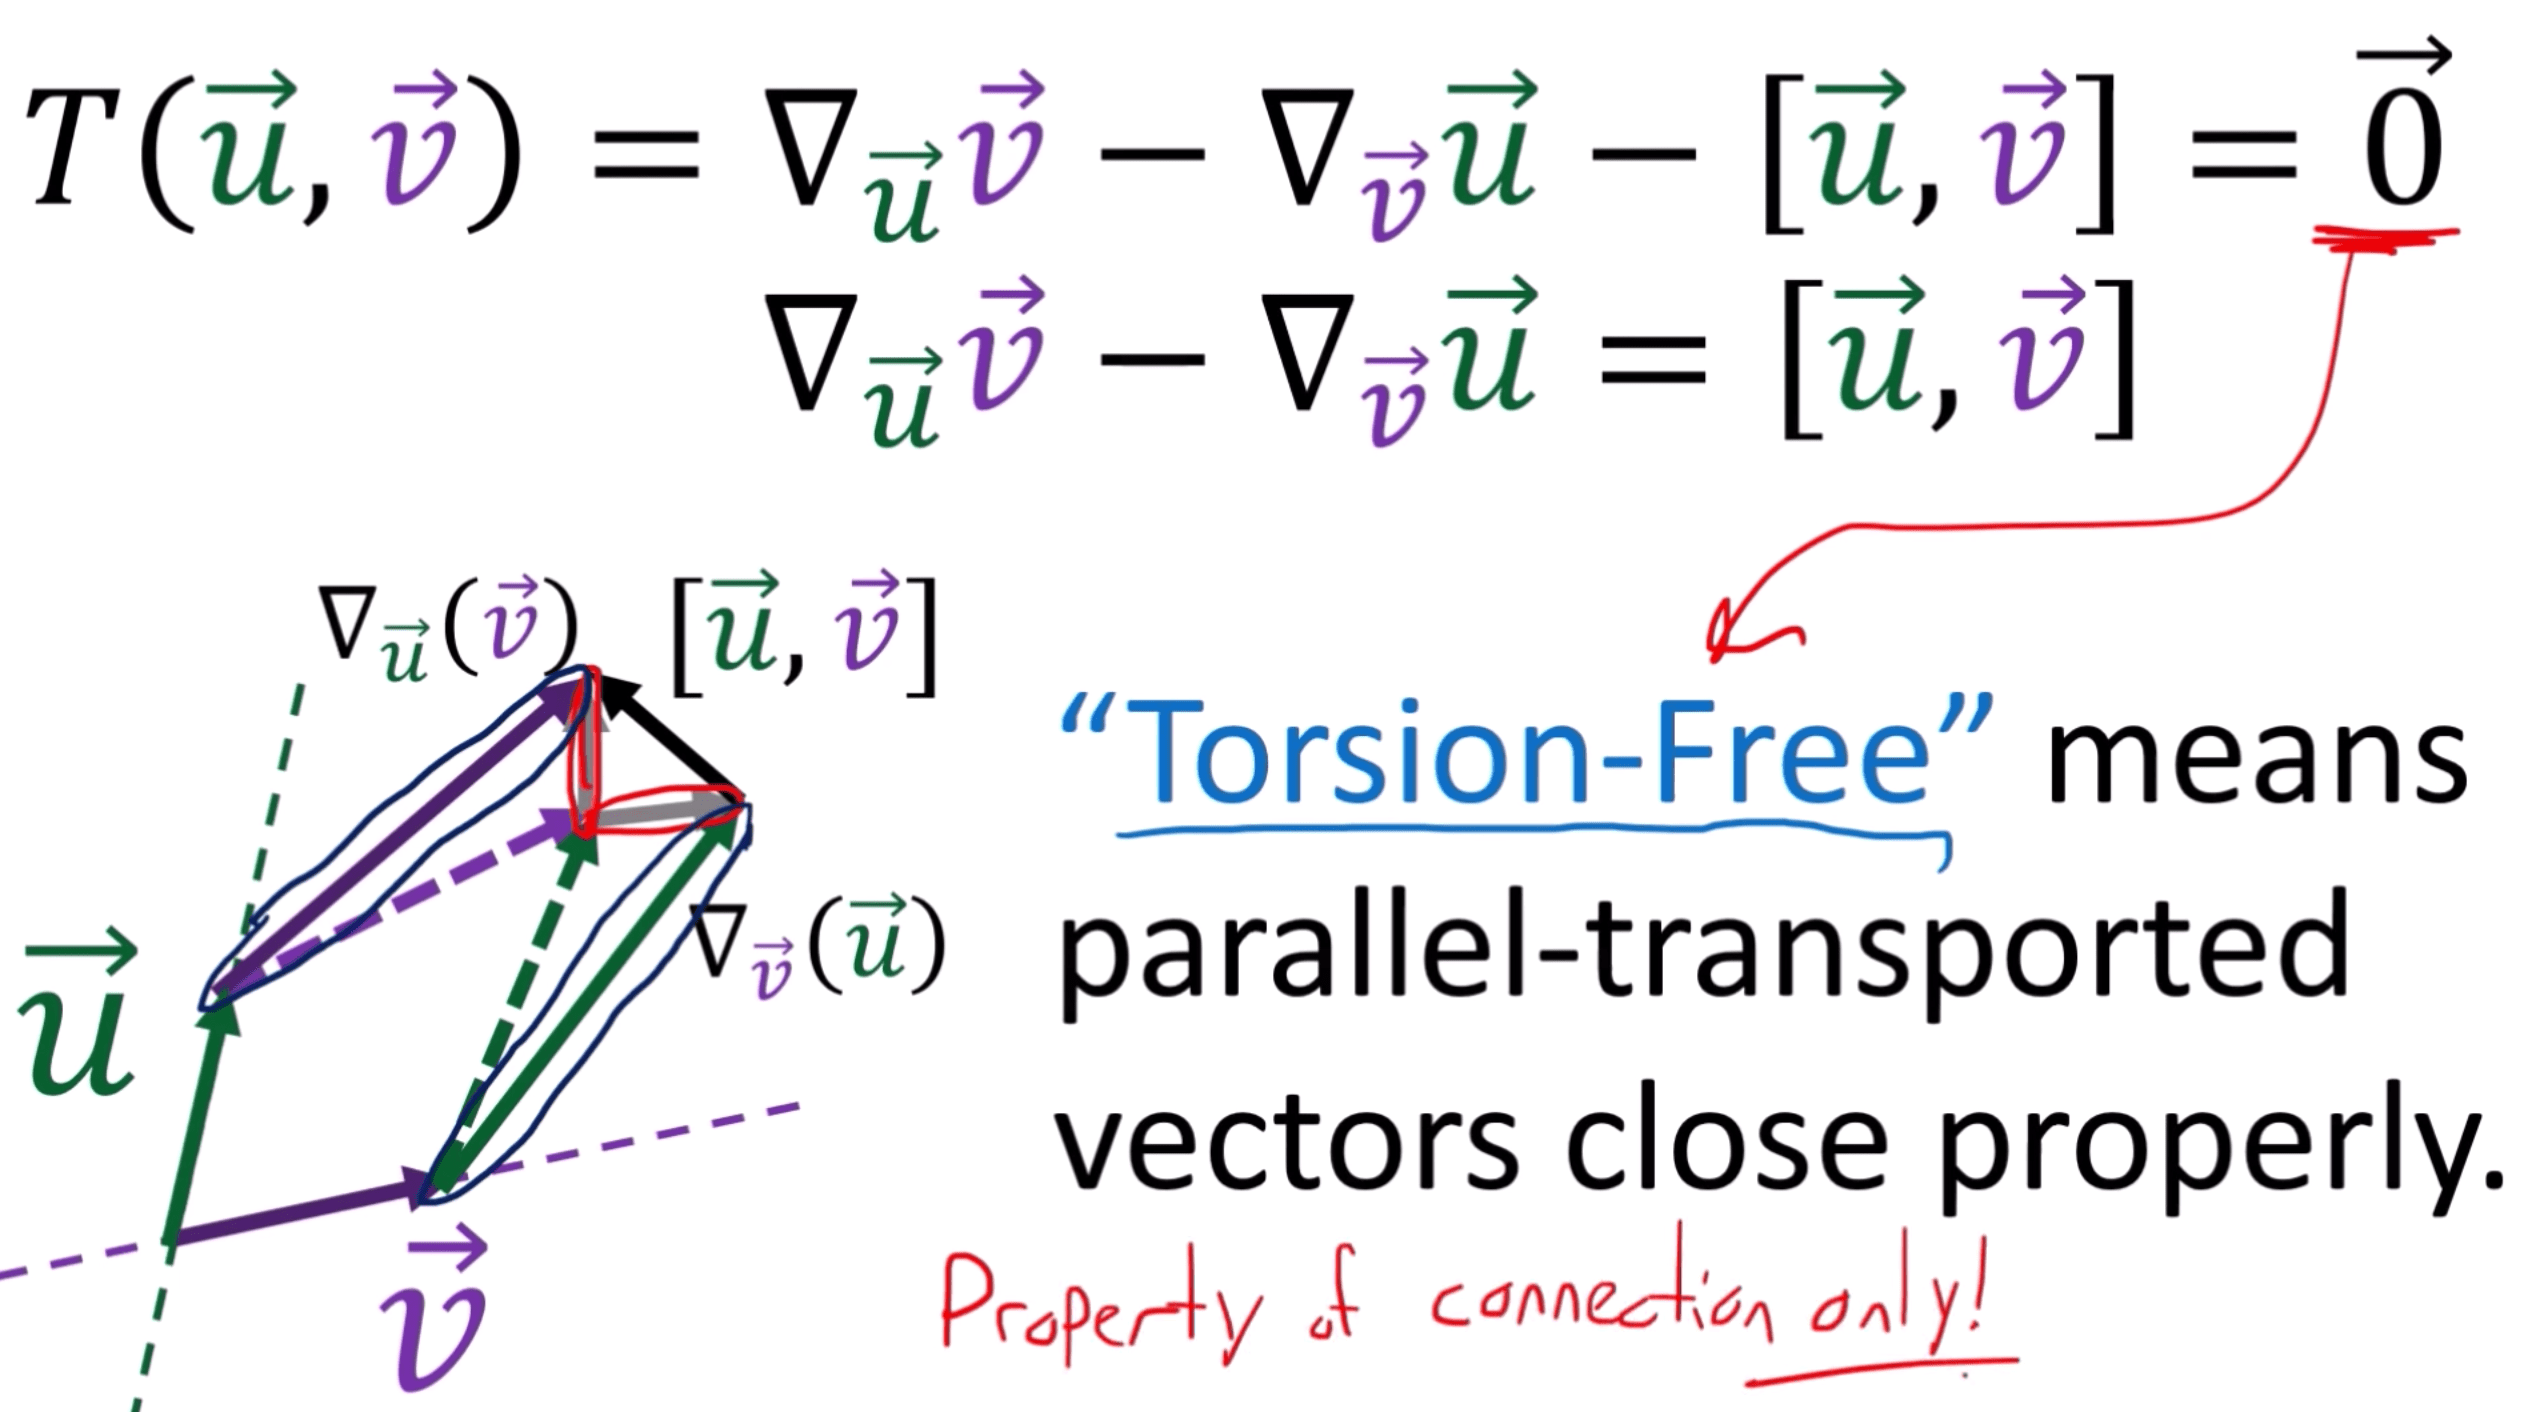
\includegraphics[width=\textwidth]{Figs/torsion2-min.png}
     \end{subfigure}
\end{figure}

\end{enumerate}

\begin{lema}\label{lem:oenqrgrgd}
 Show that a torsion free manifold is one such that the $\Gamma$s are \tb{purely symmetric}. That is ${\Gamma^i}_{[ab]} := \frac{1}{2} ({\Gamma^i}_{ab} - {\Gamma^i}_{ba}) =0$. 
\end{lema}
\begin{proof}
    We have $0=T^i_{ab}:= T(dx^i, \frac{\p}{\p^a}, \frac{\p}{\p^b})=dx^i(...)=\Gamma^i_{ab}-\Gamma^i_{ba}=2{\Gamma^i}_{[ab]}$. So it only have $\textcolor{blue}{\text{symmetric term}}$ term as shown in \cref{sec:iii}.
\end{proof}

\br 
    In most cases, we shall only use torsion free connections.
\er 
\subsection{Curvature}
There is another, more important, tensor that we can define using our connection.
\bd\bfs{Riemann Curvature}
    The \textbf{Riemann curvature} of a connection $\nabla$ is the $(1,3)$-tensor field
    \begin{align*}
        \Riem(\omega,Z,X,Y) := \omega : \big( \nabla_X\nabla_Y Z - \nabla_Y\nabla_X Z - \nabla_{[X,Y]}Z \big).
    \end{align*}
\ed 
\begin{rema}
Sometimes, we write as $R(X,Y)$ which outputs a $(1,1)$ tensor.
\end{rema}
\bd\bfs{Ricci Curvature}
    Let $\Riem$ be the Riemann curvature tensor of a connection $\nabla$. We define the \textbf{Ricci curvature} tensor as the $(0,2)$-tensor field 
    \begin{align*}
        \Ric(X,Y) := \Riem(e^a,Y,X,Z_a),
    \end{align*}
    where $e^a:Z_b = \del^a_b$.
\ed

In terms of components  the Ricci curvature tensor is given by 
\begin{align*}
    \Ric_{ab} := {\Riem^{c}}_{acb}.
\end{align*}

\bnn 
    There is a third object called the Ricci scalar (which we can't define until we have defined metrics) which we denote $R$. Seeing as it is a scalar, it has no indices and so just appears as $R$. 
\enn 

\begin{lema}
   Show that Riem is antisymmetric in its final two entries. That is 
    \begin{align*}
        \Riem(\omega,Z,X,Y) = - \Riem(\omega,Z,Y,X).
    \end{align*}
    Use this second result to show that Riem has $d^3(d-1)/2$ independent components. 
\end{lema}
\begin{proof}
    Recall the definition 
\begin{align*}
    \Riem(\omega,Z,X,Y) := \omega : \Big( \nabla_X\nabla_YZ - \nabla_Y\nabla_XZ - \nabla_{[X,Y]}Z\Big).
\end{align*}
It is easy to check that $\Riem$ is $C^{\infty}$-linear in all its entries and so we can just consider basis elements. That is, we can set (using the notation $\p_j := \frac{\p}{\p x^j}$)
\begin{align*}
    \omega = dx^i, \qquad Z = \p_j, \qquad X = \p_k, \qand Y = \p_m.
\end{align*}
So we have 
\begin{align*}
    \begin{split}
        \Riem(dx^i,\p_j,\p_k,\p_m) & := dx^i : \Big(\nabla_k\nabla_m\p_j - \nabla_m\nabla_k\p_j - \nabla_{[\p_k,\p_m]}\p_j\Big) \\ 
        & = dx^i : \Big[ \nabla_k \big(\Gamma^r_{(x)jm}\p_r\big) - \nabla_m\big( \Gamma^r_{(x)jk}\p_r\big) \Big] \\
        & = dx^i : \Big[ \Gamma^r_{(x)jm,k}\p_r + \Gamma^r_{(x)jm}\Gamma^s_{(x)rk}\p_s - \Gamma^r_{(x)jk,m}\p_r - \Gamma^r_{(x)jk}\Gamma^s_{(x)rm}\p_s \Big] \\
        {\Riem^i}_{jkm} & = \Gamma^i_{(x)jm,k} - \Gamma^i_{(x)jk,m} + \Gamma^r_{(x)jm}\Gamma^i_{(x)rk}  - \Gamma^r_{(x)jk}\Gamma^i_{(x)rm}.
    \end{split}
\end{align*}
We can see the antisymmetry in the last two entries immediatley from the above. That is ${\Riem^i}_{jkm} = -{\Riem^i}_{jmk}$.
\end{proof}

\begin{lema}
 An algebraic relevance of $\Riem$ is the following. We have the result 
\begin{align*}
    \nabla_X\nabla_YZ - \nabla_Y\nabla_X Z = \Riem(\cdot, Z,X,Y) + \nabla_{[X,Y]}Z.
\end{align*}
If we consider a chart $(U,x)$ and let $X=\p_a$ and $Y=\p_b$, this becomes 
\begin{align*}
    (\nabla_a\nabla_bZ)^m - (\nabla_b\nabla_aZ)^m = {\Riem^m}_{nab}Z^n,
\end{align*}
where we have used $[\p_a,\p_b]=0$.   
\end{lema}



\bcl \label{re:iqnne}
    The Lie bracket $[X,Y]$ answers the question of "how well the vector fields $X$ and $Y$ can be \tb{coordinate vector fields}". That is it tells us that if we lay $X$ and $Y$ on top of each other, do they form a grid? Pictorially, it asks "does the black shape close?" If $[X,Y]=0$ then the answer is yes. Note that for \tb{any chart induced coordinate map}, we have $[\p_i,\p_j]=0$, meanings  they form a grid and  must close. 
    \begin{center}
        \btik 
            \draw[thick, red, rotate around={-20:(3,0)}] (0,0) .. controls (2,0.5) and (4,0.5) .. (6,0);
            \draw[thick, red, rotate around={-20:(3,0)}, yshift = 1cm] (0,0) .. controls (2,0.5) and (4,0.5) .. (6,0);
            \draw[thick, red, rotate around={-20:(3,0)}, yshift = 2cm] (0,0) .. controls (2,0.5) and (4,0.5) .. (6,0);
            \draw[thick, red, rotate around={-20:(3,0)}, yshift = 3cm] (0,0) .. controls (2,0.5) and (4,0.5) .. (6,0);
            \node at (7.25,2) {\textcolor{red}{\Large{$X$}}};
            %
            \draw[thick, blue, rotate around={-20:(3,0)}] (0.5,-0.5) .. controls (-0.5,0.83) and (1.5,2.17) .. (0.5,4);
            \draw[thick, blue, rotate around={-20:(3,0)}, xshift = 1.5cm] (0.5,-0.5) .. controls (-0.5,0.83) and (1.5,2.17) .. (0.5,4);
            \draw[thick, blue, rotate around={-20:(3,0)}, xshift = 3cm] (0.5,-0.5) .. controls (-0.5,0.83) and (1.5,2.17) .. (0.5,4);
            \draw[thick, blue, rotate around={-20:(3,0)}, xshift = 4.5cm] (0.5,-0.5) .. controls (-0.5,0.83) and (1.5,2.17) .. (0.5,4);
            \node at (6,3) {\textcolor{blue}{\Large{$Y$}}};
            %%
            \begin{scope}
                \clip[rotate around={-20:(3,0)}] (0,2) .. controls (2,2.5) and (4,2.5) .. (6,2) -- (6,1) .. controls (4,1.5) and (2,1.5) .. (0,1) -- (0,2);
                \draw[ultra thick, rotate around={-20:(3,0)}, xshift = 1.5cm, decoration={markings, mark=at position 0.53 with {\arrow{>}}}, postaction={decorate}] (0.5,-0.5) .. controls (-0.5,0.83) and (1.5,2.17) .. (0.5,4);
                \draw[ultra thick, rotate around={-20:(3,0)}, xshift = 3cm, decoration={markings, mark=at position 0.53 with {\arrow{<}}}, postaction={decorate}] (0.5,-0.5) .. controls (-0.5,0.83) and (1.5,2.17) .. (0.5,4);
            \end{scope}
            \begin{scope}
                \clip[rotate around={-20:(3,0)}] (2,-0.5) .. controls (1,0.83) and (3,2.17) .. (2,4) -- (3.5,4) .. controls (4.5,2.17) and (2.5,0.83) .. (3.5,-0.5) -- (2,-0.5);
                \draw[ultra thick, rotate around={-20:(3,0)}, yshift = 1cm, decoration={markings, mark=at position 0.45 with {\arrow{<}}}, postaction={decorate}] (0,0) .. controls (2,0.5) and (4,0.5) .. (6,0);
                \draw[ultra thick, rotate around={-20:(3,0)}, yshift = 2cm, decoration={markings, mark=at position 0.5 with {\arrow{>}}}, postaction={decorate}] (0,0) .. controls (2,0.5) and (4,0.5) .. (6,0);
            \end{scope}
            \node at (0,2.5) {\large{$[X,Y]=0$}};
        \etik 
    \end{center}
\ecl 
From this claim we can get a nice geometrical idea for the Riemann curvature. The left-hand side ($\nabla_a\nabla_b Z-\nabla_b\nabla_aZ$) takes the vector $Z$ from the bottom corner of the black shape and around in the direction of the arrows drawn (note the minus sign means we go down the $X$ and left on the $Y$). 
\begin{itemize}
    \item If Riem vanishes, the result is that the transported $Z$ and the initial $Z$ coincide, and therefore we haven't travelled through curvature (recall that parallel transport on a curved surface is path dependent). 
    \item Whereas if Riem does not vanish then the transported $Z$ is not the same as the initial $Z$ and so \tb{we must have gone through curvature}. 
\end{itemize}Therefore the Riemann curvature tensor encodes information about the curvature of the manifold (hence the name!).

\br 
    Note we have used a chart in order to obtain the above result and so we might be worried that Riem vanishes in one chart but not in another (e.g. Cartesian to polar). The answer is obviously that this can't happen because it is a tensor and so if it vanishes in one chart it must vanish in all charts.
\er 

\bl 
    The Riemann tensor satisfies the differential \textbf{Bianchi identity}, 
    \begin{align*}
        (\nabla_A\Riem)(\omega,Z,B,C) + (\nabla_B\Riem)(\omega,Z,C,A) + (\nabla_C\Riem)(\omega,Z,A,B) = 0,
    \end{align*}
    where $\nabla$ is torsion-free. In component form this reads 
    \begin{align*}
        \nabla_c{R^w}_{zab} + \nabla_a{R^w}_{zbc} + \nabla_b{R^w}_{zca} = 0 
    \end{align*}
\el 



\section{Metric Manifolds}
We establish a structure on a smooth manifold $(\cM,\cO,\cA)$ that allows us to assign vectors in each tangent space a length and\footnote{If we were only looking to define a length, we would just define a norm on our manifold. For more information on norms see Dr. Schuller's Lectures on Quantum Theory.} an angle between vectors in the same tangent space. Such a structure in each tangent space is a \textit{inner product}, and the complete structure over all tangent spaces is what we call a \textit{metric} (i.e. it is a inner produce field). 

From this structure, one can then define a notion of length of a curve. Then we can look at shortest (and longest) curves, which are known as \textit{geodesics}. We will develop this completely independently of the notion of straight curves, i.e. of the  covariant derivative, but then shall insist, for obvious reasons, at the end that the two coincide. In doing this we will define what we mean by so-called \textit{metric compatible} connections.

\subsection{Metrics}

\bd[Metric]
    A \textbf{metric} $g$ on a smooth manifold $(\cM,\cO,\cA)$ is a $(0,2)$-tensor field satisfying:
    \benr 
        \item It's symmetric; $g(X,Y) = g(Y,X)$, for all $X,Y\in\Gamma T\cM$, and
        \item Non-degeneracy; the map $\flat : \Gamma T\cM\to \Gamma T^*\cM$, given by 
        \begin{align*}
            \flat(X) :Y := g(X,Y),
        \end{align*}
        is a $C^{\infty}$-isomorphism, i.e. it is invertible and smooth in both directions. 
    \een 
\ed 

\subsection{Isometry}
\begin{defa}\bfs{Isometry}
Suppose $(M, g)$ and $(\widetilde{M}, \widetilde{g})$ are Riemannian manifolds with or without boundary. An \tb{isometry} from $(\boldsymbol{M}, \boldsymbol{g})$ to $(\widetilde{\boldsymbol{M}}, \widetilde{\boldsymbol{g}})$ is a \tb{diffeomorphism} $\varphi: M \rightarrow \widetilde{M}$ such that $\varphi^{*} \widetilde{g}=g$ (see \cref{def:dfafrerq} {induced metric}). 

Namely, $\varphi$ is a smooth bijection and each differential $d \varphi_{p}: T_{p} M \rightarrow T_{\varphi(p)} \widetilde{M}$ be a \tb{linear isometry}. We say $(M, g)$ and $(\widetilde{M}, \widetilde{g})$ are isometric if there exists an isometry between them.
\end{defa}
\begin{rema}
 Riemannian geometry, is concerned primarily with properties of Riemannian manifolds that are preserved by isometries. A composition of isometries and the inverse of an isometry are again isometries, so being isometric is an equivalence relation on the class of Riemannian manifolds with or without boundary. 
\end{rema}
\begin{defa}\bfs{Local Isometry}
If $(M, g)$ and $(\widetilde{M}, \widetilde{g})$ are Riemannian manifolds, a map $\varphi: M \rightarrow \widetilde{M}$ is a local isometry if each point $p \in M$ has a neighborhood $U$ such that $\left.\varphi\right|_{U}$ is an isometry onto an open subset of $\widetilde{M}$.
\end{defa}
\begin{lema}
 If $(M, g)$ and $(\widetilde{M}, \tilde{g})$ are Riemannian manifolds of the same dimension, a smooth map $\varphi: M \rightarrow \mathscr{M}$ is a local isometry if and only if $\varphi^{*} \tilde{g}=g$.
\end{lema}
\begin{defa}\bfs{flat}
A Riemannian $n$-manifold is said to be flat if it is locally isometric to a Euclidean space, that is, if every point has a neighborhood that is isometric to an open set in
\end{defa}

\subsection{Raising and Lowering Indices}
One elementary but important property of Riemannian metrics is that they allow us to convert vectors to covectors and vice versa. Raising and lowering indices refers to the component of (co)vectors. Recall that \tb{vectors components have upper indices; covectors components have lower indices.}

$\bullet$ \tb{Lowering Indices: get covector field from vector field}

\begin{defa}
Given a Riemannian metric $g$ on $M$, we define a bundle homomorphism $\hat{g}: T M \rightarrow T^{*} M$ by setting
\begin{align*}
\widehat{g}(v)(w)=g_{p}(v, w)
\end{align*}
for all $p \in M$ and $v, w \in T_{p} M$. If $X$ and $Y$ are smooth vector fields on $M$, this yields
\begin{align*}
\widehat{g}(X)(Y)=g(X, Y),
\end{align*}
\end{defa}


Given a smooth local frame $\left(E_{i}\right)$ and its dual coframe $\left(\varepsilon^{i}\right)$, let $g=g_{i j} \varepsilon^{i} \varepsilon^{j}$ be the local expression for $g$. If $X=X^{i} E_{i}$ is a smooth vector field, the covector field $\widehat{g}(X)$ has the coordinate expression
\begin{align*}
\widehat{g}(X)=\left(g_{i j} X^{i}\right) \varepsilon^{j}
\end{align*}
Thus the matrix of $\hat{g}$ in any local frame is the same as the matrix of $g$ itself.
Given a vector field $X$, it is standard practice to denote the components of the covector field $\widehat{g}(X)$ by
\begin{align*}
X_{j}=g_{i j} X^{i}
\end{align*}
so that
\begin{align*}
X^{\flat}:=\widehat{g}(X)=X_{j} \varepsilon^{j}.
\end{align*}

$\bullet$ \tb{Raising Indices:  get vector field from covector field}
\bd[Inverse Metric] 
    The \textbf{inverse metric}, $g^{-1}:\Gamma T^*\cM\times \Gamma T^*\cM\lmap C^{\infty}(\cM)$, w.r.t. a metric $g$ is the symmetric, $(2,0)$-tensor field defined by 
    \begin{align*}
        g^{-1}(\omega,\sig) := \omega : \flat^{-1}(\sig).
    \end{align*}
\ed 

\br 
    One needs to be careful when referring to $g^{-1}$ as an inverse. It is not an inverse in the sense of a map, but in the matrix sense. That is the map inverse of $g:\Gamma T\cM\times \Gamma T\cM\lmap C^{\infty}(\cM)$ would be a map from $\C^{\infty}(\cM)$ to $\Gamma T\cM\times\Gamma T\cM$, which $g^{-1}$ is not. If we denote the components of $g^{-1}$ simply as $g^{ab}$ (so no $-1$ in it), then what we mean by inverse is that the following holds:
    \begin{align*}
        g^{ac}g_{cb} = \del^a_b.
    \end{align*}
\er 

% Because the matrix $\left(g_{i j}\right)$ is nonsingular at each point, the map $\hat{g}$ is invertible, and the matrix of $\hat{g}^{-1}$ is just the inverse matrix of $\left(g_{i j}\right)$. We denote this inverse matrix by $\left(g^{i j}\right)$, so that $g^{i j} g_{j k}=g_{k j} g^{j i}=\delta_{k}^{i}$. The symmetry of $g_{i j}$ easily implies that $\left(g^{i j}\right)$ is also symmetric in $i$ and $j$. 

In terms of a local frame, the inverse map $\widehat{g}^{-1}$ is given by
\begin{align*}
\omega^{\sharp}:=\widehat{g}^{-1}(\omega)=\omega^{i} E_{i}
\end{align*}
where
\begin{align*}
\omega^{i}=g^{i j} \omega_{j} .
\end{align*}

\begin{defa}\bfs{musical isomorphisms}
The two inverse isomorphisms $b$ and $\sharp$ are known as the \tb{musical isomorphisms.}
\end{defa}

Probably the most important application of the sharp operator is to extend the classical gradient operator to Riemannian manifolds. If $g$ is a Riemannian metric

\subsection{Gradient, Divergence and Laplacian}
\begin{defa}\bfs{Gradient}
If $g$ is a Riemannian metric on $M$ and $f: M \rightarrow \mathbb{R}$ is a smooth function, the \tb{gradient of $f$ is the vector field} $\operatorname{grad} f=(d f)^{\sharp}$ obtained from $d f$ by raising an index. Unwinding the definitions, we see that  $\operatorname{grad} f$ is characterized by the fact that
\begin{align*}
d f_{p}(w)=\left\langle\left.\operatorname{grad} f\right|_{p}, w\right\rangle \quad \text { for all } p \in M, w \in T_{p} M
\end{align*}
and has the local basis expression
\begin{align*}
\operatorname{grad} f=\left(g^{i j} E_{i} (f)\right) E_{j}
\end{align*}
Note that then 
\begin{align*}
\left\langle\left.\operatorname{grad} f\right|_{p}, w\right\rangle &=\left\langle\left(g^{i j} E_{i} (f)\right) E_{j}, \varepsilon^{i} (w)E_{i} \right\rangle\\
& = E_i(f) \varepsilon^i(w) \\
& = df(w)\\
&= W^i \frac{\p f}{\p x^i}  \text{ if we use a local chart based basis}
\end{align*}
\end{defa}
\begin{lema}
 If $\left(E_{i}\right)$ is an orthonormal frame, then $\operatorname{grad} f$ is the vector field whose components are the same as the components of $d f$; but in other frames, this will not be the case.
\end{lema}
\begin{defa}\bfs{Divergence}
Suppose $(M, g)$ is an oriented Riemannian $n$-manifold with or without boundary, and $d V_{g}$ is its volume form. If $X$ is \tb{ a smooth vector field} on $M$, then $\left.X\right\lrcorner d V_{g}$ is an $(n-1)$-form. The exterior derivative of this $(n-1)$-form is a smooth $n$-form, so it can be expressed as a \tb{smooth function} multiplied by $d V_{g}$. \tb{That function} is called the \tb{divergence} of $\boldsymbol{X}$, and denoted by $\operatorname{div} X$; thus it is characterized by the following formula:
\begin{align*}
\left.d(X\lrcorner d V_{g}\right)=(\operatorname{div} X) d V_{g} .
\end{align*}
\end{defa}
% Even if $M$ is nonorientable, in a neighborhood of each point we can choose an orientation and define the divergence by (2.19), and then note that reversing the orientation changes the sign of $d V_{g}$ on both sides of the equation, so $\operatorname{div} X$ is well defined, independently of the choice of orientation. In this way, we can define the divergence operator on any Riemannian manifold with or without boundary, by requiring that it satisfy (2.19) for any choice of orientation in a neighborhood of each point.

% The most important application of the divergence operator is the divergence theorem, which you will be asked to prove in Problem 2-22.
\begin{defa}\bfs{Laplacian}
Using the divergence operator, we can define another important operator, this one acting on real-valued functions. The Laplacian (or Laplace-Beltrami operator) is the \tb{linear operator $\Delta: C^{\infty}(M) \rightarrow C^{\infty}(M)$} defined by
\begin{align*}
\Delta u=\operatorname{div}(\operatorname{grad} u) .
\end{align*}
\end{defa}

\begin{lema}
 Let $(M, g)$ be a Riemannian manifold with or without boundary, and let $\left(x^{i}\right)$ be any smooth local coordinates on an open set $U \subseteq M$. The coordinate representations of the divergence and Laplacian are as follows:

\begin{align*}
\begin{aligned}
\operatorname{div}\left(X^{i} \frac{\partial}{\partial x^{i}}\right) &=\frac{1}{\sqrt{\operatorname{det} g}} \frac{\partial}{\partial x^{i}}\left(X^{i} \sqrt{\operatorname{det} g}\right) \\
\Delta u &=\frac{1}{\sqrt{\operatorname{det} g}} \frac{\partial}{\partial x^{i}}\left(g^{i j} \sqrt{\operatorname{det} g} \frac{\partial u}{\partial x^{j}}\right)
\end{aligned}
\end{align*}
where $\operatorname{det} g=\operatorname{det}\left(g_{k l}\right)$ is the determinant of the component matrix of $g$ in these coordinates. On $\mathbb{R}^{n}$ with the Euclidean metric and standard coordinates, these reduce to
\begin{align*}
\begin{aligned}
\operatorname{div}\left(X^{i} \frac{\partial}{\partial x^{i}}\right) &=\sum_{i=1}^{n} \frac{\partial X^{i}}{\partial x^{i}} \\
\Delta u &=\sum_{i=1}^{n} \frac{\partial^{2} u}{\left(\partial x^{i}\right)^{2}}
\end{aligned}
\end{align*}
\end{lema}
\begin{thma}
Suppose $(M, g)$ is a compact Riemannian manifold with boundary.
\begin{enumerate}[(a)]
    \item Prove the following divergence theorem for $X \in X(M)$ :
\begin{align*}
\int_{M}(\operatorname{div} X) d V_{g}=\int_{\partial M}\langle X, N\rangle_{g} d V_{\widehat{g}}
\end{align*}
where $N$ is the outward unit normal to $\partial M$ and $\hat{g}$ is the induced metric on $\partial M$. [Hint: Prove it first in the case that $M$ is orientable, and then apply that case to the orientation covering of $M$ (Prop. B.18).]
\item Show that the divergence operator satisfies the following product rule for $u \in C^{\infty}(M)$ and $X \in \mathfrak{X}(M)$ :
\begin{align*}
\operatorname{div}(u X)=u \operatorname{div} X+\langle\operatorname{grad} u, X\rangle_{g},
\end{align*}
and deduce the following "integration by parts" formula:
\begin{align*}
\int_{M}\langle\operatorname{grad} u, X\rangle_{g} d V_{g}=\int_{\partial M} u\langle X, N\rangle_{g} d V_{\widehat{g}}-\int_{M} u \operatorname{div} X d V_{g} .
\end{align*}
What does this say when $M$ is a compact interval in $\mathbb{R}$ ?
\end{enumerate}
\end{thma}

\subsection{Length of A Curve}

Let $\gamma:\R\to\cM$ be a smooth curve, then we know its velocity $v_{\gamma,\gamma(\lambda)}$ at each $\gamma(\lambda)\in\cM$. On a topological manifold this is as far as we can go, but on a metric manifold we have the following. 

\bd\bfs{Speed of a Curve}
    On a Riemannian metric manifold $(\cM,\cO,\cA,g)$, the \textbf{speed} of a curve at $\gamma(\lambda)$ is the number 
    \begin{align*}
        s(\lambda) := \sqrt{g(v_{\gamma},v_{\gamma})}\Big|_{\gamma(\lambda)}
    \end{align*}
\ed  
\bd
    Let $\gamma: (0,1) \to \cM$\footnote{We are free to choose the domain of $\gamma$ to be $(0,1)$ by simply rescalling/shifting $\lambda$ accordingly.} be a smooth curve. Then the \textbf{length} of $\gamma$ is the number\footnote{We have used square brackets around $\gamma$ below because it is a function. This tells us that $L$ is a so-called \textit{functional}. Anyone unfamiliar with this terminology is referred to a course on Lagrangian mechanics.}
    \begin{align*}
        L[\gamma] := \int_0^1 d\lambda \, s(\lambda).
    \end{align*}
\ed 
\bt \bfs{reparameter}
    Let $\gamma:(0,1) \to \cM$ be a smooth curve and let $\sig:(0,1)\to(0,1)$ be smooth, bijective and increasing, then $L[\gamma] = L[\gamma\circ\sig]$.
\et 
\begin{proof}
    Using 
\begin{align*} 
    \cL[\gamma] = \sqrt{g(v_{\gamma},v_{\gamma})}, \qand \dot{\widetilde{\gamma}}^a(\lambda) = (x^a\circ \gamma)'(\lambda),
\end{align*} 
and introducing the notation 
\begin{align*} 
    \widetilde{\lambda} := \sig(\lambda), \qquad \implies \qquad \widetilde{\gamma}(\lambda) = \gamma(\widetilde{\lambda}),
\end{align*} 
we have 
\begin{align*} 
    \begin{split}
        L[\widetilde{\gamma}] & := \int_0^1 d\lambda \sqrt{g(v_{\widetilde{\gamma}},v_{\widetilde{\gamma}})} \\
        & = \int_0^1 d\lambda \sqrt{g_{ab}\big(\widetilde{\gamma}(\lambda)\big)\cdot\dot{\widetilde{\gamma}}^a(\lambda) \cdot  \dot{\widetilde{\gamma}}^b}(\lambda) \\
        & = \int_0^1 d\lambda \sqrt{g_{ab}\big(\gamma(\widetilde{\lambda})\big) \cdot (x^a\circ \gamma \circ \sig)'(\lambda) \cdot (x^b\circ \gamma \circ \sig)'(\lambda)} \\
        & = \int_0^1 d\lambda \sqrt{g_{ab}\big(\gamma(\widetilde{\lambda})\big) \cdot (x^a\circ \gamma)'(\widetilde{\lambda})\cdot \dot{\sig}(\lambda) \cdot (x^b\circ \gamma)'(\widetilde{\lambda)}\cdot\dot{\sig}(\lambda)} \\
        & = \int_0^1 d\lambda \dot{\sig}(\lambda)\sqrt{g_{ab}\big(\gamma(\widetilde{\lambda})\big) \cdot \dot{\gamma}^a(\widetilde{\lambda}) \cdot \dot{\gamma}^b(\widetilde{\lambda})} \\
        & = \int_0^1 d\widetilde{\lambda} \sqrt{g_{ab}\big(\gamma(\widetilde{\lambda})\big) \cdot \dot{\gamma}^a(\widetilde{\lambda}) \cdot \dot{\gamma}^b(\widetilde{\lambda})} \\
        & = L[\gamma],
    \end{split}
\end{align*} 
where we have used the chain rule, and the result $d\widetilde{\lambda} = \dot{\sig}d\lambda$.
\end{proof}

\subsection{Geodesics: note here is miminal }

\bd[Geodesic]
    A curve $\gamma:(0,1)\to\cM$ is called a \textbf{geodesic} on a Riemannian manifold $(\cM,\cO,\cA,g)$ if it is a \textit{stationary}\footnote{In the sense of Lagrangians in classical mechanics.} curve w.r.t. the length functional $L$.
\ed

\bt 
    The curve $\gamma:(0,1)\to\cM$ is a geodesic if and only if it satisfies the Euler Lagrange equations for the Lagrangian \begin{align*}
        \begin{split}
            \cL : T\cM &\to \R \\
            X &\mapsto \sqrt{g(X,X)}.
        \end{split}
    \end{align*}
    In a chart, this is 
    \begin{align*}
        \cL(\gamma^i,\Dot{\gamma}^i) = \sqrt{g_{ij}\big(\gamma(\lambda)\big)\Dot{\gamma}^i(\lambda)\Dot{\gamma}^j(\lambda)}.
    \end{align*}
\et 

Finding the Euler Lagrange equations proceeds as follows:
\begin{align*}
    \begin{split}
        \frac{\p\cL}{\p\Dot{\gamma}^m} & = \frac{1}{\sqrt{...}} g_{mj}\big(\gamma(\lambda)\big) \Dot{\gamma}^j(\lambda) \\
        \therefore \frac{d}{d\lambda}\bigg(\frac{\p\cL}{\p\Dot{\gamma}^m}\bigg) & = \frac{d}{d\lambda}\bigg(\frac{1}{\sqrt{...}}\bigg) g_{mj}\big(\gamma(\lambda)\big) \Dot{\gamma}^j(\lambda) + \frac{1}{\sqrt{...}} \Big( g_{mj}\big(\gamma(\lambda)\big) \Ddot{\gamma}^j(\lambda) + \Dot{\gamma}^s(\lambda)\big[\p_s g_{mj}\big(\gamma(\lambda)\big)\big] \Dot{\gamma}^j(\lambda) \Big).
    \end{split}
\end{align*}
Now we're stuck with the ugly task of trying to work out $\frac{d}{d\lambda}\Big(\frac{1}{\sqrt{...}}\Big)$. However, we have already demonstrated that the length of the curve is independent on how we choose to our parameter. We are free, therefore, to choose it to be something convenient, and we simply take it to be such that $g(\Dot{\gamma},\Dot{\gamma})=1$, that is the speed it one along the whole curve. We then just have 
\begin{align*}
    \frac{d}{d\lambda}\bigg(\frac{\p \cL}{\p \Dot{\gamma}^m}\bigg) = g_{mj}\big(\gamma(\lambda)\big) \Ddot{\gamma}^j(\lambda) + \Dot{\gamma}^s(\lambda)\Big(\p_s g_{mj}\big(\gamma(\lambda)\big)\Big) \Dot{\gamma}^j(\lambda).
\end{align*}
We also need to find 
\begin{align*}
    \frac{\p \cL}{\p \gamma^m} = \frac{1}{2} \Big(\p_m g_{ij}\big(\gamma(\lambda)\big)\Big) \Dot{\gamma}^i(\lambda) \Dot{\gamma}^j(\lambda),
\end{align*}
where we have already imposed our parameter choice condition. So our \tb{Euler Lagrange equations} are (dropping the $(\lambda)$s for notational brevity)
\begin{align*}
    g_{mj}\Ddot{\gamma}^j + (\p_ig_{mj})\dot{\gamma}^i\Dot{\gamma}^j - \frac{1}{2}(\p_mg_{ij})\Dot{\gamma}^i\Dot{\gamma}^j = 0.
\end{align*}
Multiplying both sides by the inverse metric $g^{mq}$ and using the condition $g^{mq}g_{mj}=\del^q_j$, we have 
\begin{align*}
    \Ddot{\gamma}^q + g^{qm}\bigg( \p_ig_{mj} - \frac{1}{2}\p_mg_{ij}\bigg) \dot{\gamma}^{(i}\dot{\gamma}^{j)} = 0,
\end{align*}
where the brackets on the last two indices indicate the symmetry $\dot{\gamma}^i\dot{\gamma}^j = \dot{\gamma}^j\dot{\gamma}^i$. Using this symmetry we can double the first term by switching $i\leftrightarrow j$, giving us 
\begin{align*}
    \Ddot{\gamma}^q + \frac{1}{2}g^{qm}\big(\p_ig_{mj}+\p_jg_{mi} - \p_mg_{ij}\big)\dot{\gamma}^{(i}\dot{\gamma}^{j)} = 0.
\end{align*}
This is the \textbf{geodesic equation} for the components of $\gamma$ in a chart. 

We can write this in the form of an autoparallel\footnote{I.e. in the form $\Ddot{\gamma}^q + {\Gamma^q}_{ij}\dot{\gamma}^i\dot{\gamma}^j$.} equation by introducing the following definition.
\bd\bfs{Levi-Civita connection coefficients}
    Given a metric $g$ and a chart $(U,x)$, we define the  \textbf{Levi-Civita connection coefficients} as 
    \begin{align*}
        ^{LC}{\Gamma^q}_{ij}\big(\gamma(\lambda)\big) := \frac{1}{2}g^{qm}\big(\p_ig_{mj}+\p_jg_{mi} - \p_mg_{ij}\big),
    \end{align*}
    where the components of the metric (and its inverse, obviously) are taken in the chart given. 
\ed 
It is important to note, though, that \tb{up until this point, geodesics and autoparallels are completely separate entities.}

Note by making this identification, we obtain the connection \textit{from} the metric. That is, we do not need to provide both a metric and a connection, but by simply providing a metric we can obtain a unique connection such that the shortest curves and the  straight curves coincide:
\bt 
    Let $(\cM,\cO,\cA,g,\nabla)$ be a topological manifold equipped with both a metric and a connection. If
    \benr 
        \item $\nabla$ is \textit{torsion free}, and 
        \item $\nabla g = 0$, known as \textit{metric compatibility},
    \een 
    then we can conclude $\nabla = ^{LC}\nabla$.
\et 

\bq 

 Expand in terms of connection coefficient functions 
 $\big(\nabla_ag\big)_{bc}$, 
    $\big(\nabla_bg\big)_{ca}$,
 $\big(\nabla_cg\big)_{ab}$:
\begin{align*} 
    \big(\nabla_ag\big)_{bc} = g_{bc,a} - {\Gamma^m}_{ba}g_{mc} - {\Gamma^m}_{ca}g_{bm}. 
\end{align*}
Consider $\big(\nabla_ag\big)_{bc}+\big(\nabla_bg\big)_{ca}-\big(\nabla_cg\big)_{ab}$:
\begin{align*} 
    g_{bc,a} - {\Gamma^m}_{ba}g_{mc} - {\Gamma^m}_{ca}g_{bm} + g_{ca,b} - {\Gamma^m}_{cb}g_{ma} - {\Gamma^m}_{ab}g_{cm} - g_{ab,c} + {\Gamma^m}_{ac}g_{mb} + {\Gamma^m}_{bc}g_{am}.
\end{align*} 
Now if we consider a metric compatible connection and vanishing torsion, we have that the above vanishes (as each of three terms vanish) and that the $\Gamma$s are symmetric in the lower two indices. Also using the fact that the metric is symmetric, we have 
\begin{align*} 
    0 = g_{bc,a} + g_{ac,b} - g_{ab,c} - 2{\Gamma^m}_{ba}g_{mc},
\end{align*} 
which after rearranging and using $g_{mc}g^{-1})^{cn} = \del^n_m$ we have 
\begin{align*} 
    {\Gamma^n}_{ba} = \frac{1}{2}\big(g^{-1}\big)^{cn}\big(g_{bc,a} + g_{ac,b} - g_{ab,c}\big),
\end{align*} 
which, relabelling $n\to a \to c \to m$ gives
\begin{align*} 
    {\Gamma^a}_{bc} = \frac{1}{2}\big(g^{-1}\big)^{ma}\big(g_{bm,c} + g_{cm,b} - g_{cb,m}\big)
\end{align*} 
which is the result (when you us the symmetries). So we see the connection coefficient functions are uniquely determined by the metric components given the above conditions. 
\eq 
\begin{rema}\bfs{metric compatibility explanation}
Metric compatibility can be also write as:
$$
\nabla_{\vec{w}}(\vec{v} \cdot \vec{u})=\left(\nabla_{\vec{w}} \vec{v}\right) \cdot \vec{u}+\vec{v} \cdot\left(\nabla_{\vec{w}} \vec{u}\right)
$$
It means "when we parallel transport two vectors, their dot product will stay the same." In other words: if  $\nabla_{\vec{w}} \vec{v}=\overrightarrow{0}$ and  $\nabla_{\vec{w}} \vec{u}=\overrightarrow{0}$, we then have $\nabla_{\vec{w}}(\vec{v} \cdot \vec{u})^{2}=\overrightarrow{0}$ keeps a constant. It can be show that the angle between two parallel transported vector along a curve  and the length of the two vectors will keep fixed during the  parallel transport.
\end{rema}


Finally let's introduce some definitions. As we see, all of them are directly related to the metric.

\bd[Riemann Christoffel Curvature]
    Let $(\cM,\cO,\cA,g)$ be a metric manifold. The components of the  \textbf{Riemann Christoffel curvature} are defined by  
    \begin{align*}
        \Riem_{abcd} := g_{am}{\Riem^m}_{bcd},
    \end{align*}
    where ${\Riem^m}_{bcd}$ are the Riemann tensor components obtained from the Levi-Civita connection $^{LC}\nabla$. 
\ed 

\bd[Ricci Scalar]
    Let $(\cM,\cO,\cA,g)$ be a metric manifold and let $\Riem$ be the Riemann tensor obtained from the Levi-Civita connection. We then define the \textbf{Ricci scalar} as 
    \begin{align*}
        R = g^{ab}\Ric_{ab},
    \end{align*}
    where $\Ric_{ab}:={\Riem^c}_{acb}$ are the components of the Ricci curvature tensor.
\ed 

\bd[Einstein Curvature]
    Let $(\cM,\cO,\cA,g)$ be a metric manifold and let $\Riem$ be the Riemann tensor obtained from the Levi-Civita connection. We define the components of the \textbf{Einstein curvature} as
    \begin{align*}
        G_{ab} := \Ric_{ab} - \frac{1}{2}g_{ab}R,
    \end{align*}
    where $\Ric$ and $R$ are the Ricci curvature and Ricci scalar, respectively.
\ed 
\begin{rema}
 It is important to note that these quantities are not only related to the metric through its direct appearance in the expressions, but also through the fact that, in order to define the Riemann curvature tensor we need a connection and for all of them we used the Levi-Civita connection, a metric dependent object. For this latter reason, the Ricci curvature tensor (defined previously) is also a metric dependent object.
\end{rema}
\br 
    The above definitions can, of course, all be expressed in a chart free manner as they are tensors, however the notation can be a bit confusing and it's much easier to see in component form, hence why we have defined it this way. 
\er 
\section{Symmetry}
$\bullet$ \tb{Motivation:}

We have the intuitive feeling that the round sphere of radius $R$, $(S^2,\cO,\cA,g^{\text{round}})$, has \textit{rotational symmetry}, while the potato $(S^2,\cO,\cA,g^{\text{potato}})$ does not. 

Prior to this course we have been taught  to think of symmetries as a group of maps which map the object to itself, while preserving all of the structures of the object. In most cases, we make use of the inner product available to us. The method we're about to describe here is actually subtly different. First, from different metric structure $g^{\text{round}}$ and $g^{\text{potato}}$ on the manifold, we get the feeling of the symmetry, it is not from some innner product. Second, give a metric, there are lots of local inner product, the symmetries appear to come from their \tb{distribution over the manifold}. So we want to answer the question `how do we describe the symmetries of a metric?' 
\subsection{Push-Forward Map: vectors are pushed forward}\label{sec:pushforward}
\bd\bfs{Push-Forward Map}
    Let $\phi:\cM\to\cN$ be a smooth map between two smooth manifolds. Then we define the \textbf{push-forward map} $\phi_* : T\cM \to T\cN $ by 
    \begin{align*}
        \phi_*(X)\la f \ra  := X \la f \circ \phi \ra,
    \end{align*}
    where $f\in C^{\infty}(\cN)$, i.e. $f:\cN\to\R$. 
\ed 
Diagrammatically, the maps in the above definition are related by the following diagram. 
\begin{center}
    \btik 
        \draw[thick, ->] (0,0) -- (3,0) node[label={above:\large $\phi_*$}, midway]{};
        \draw[thick, ->] (-0.5,-0.5) -- (-0.5,-1.5) node[label={left:\large $\pi_{\cM}$}, midway]{};
        \draw[thick, ->] (3.5,-0.5) -- (3.5,-1.5) node[label={right:\large $\pi_{\cN}$}, midway]{};
        \draw[thick, ->] (0,-2) -- (3,-2) node[label={above:\large $\phi$}, midway]{};
        \draw[thick, ->] (4,-2) -- (5.5,-2) node[label={above:\large $f$}, midway]{};
        \node at (-0.5,0) {\large{$T\cM$}};
        \node at (3.5,0) {\large{$T\cN$}};
        \node at (-0.5,-2) {\large{$\cM$}};
        \node at (3.5,-2) {\large{$\cN$}};
        \node at (6,-2) {\large{$\R$}};
    \etik 
\end{center}

\bc 
    Recall that the fibres of the tangent bundle are just the tangent spaces to that point, i.e. $\preim_{\pi_{\cM}}p = T_p\cM$. It follows, then, that 
    \begin{align*} 
        \phi_* \big(T_p\cM\big) \se T_{\phi(p)}\cN.
    \end{align*} 
    That is, the image of the $p$-fibres on $\cM$ are at least contained within the $\phi(p)$-fibres on $\cN$.
\ec 
\begin{rema}
 There is a mnemonic to remember what the push forward does: \tb{``vectors are pushed forward''.}
\end{rema}


It is worth looking at the components of the push-forward map in the \textit{two} charts $(U,x)\in\cA_{\cM}$ and $(V,y)\in\cA_{\cN}$. We have, for $p\in\cM$ 
\begin{align*} 
    \begin{split}
        \phi^{\,\,a}_{*\,\,i} := dy^a : \phi_*\Bigg(\bigg(\frac{\p}{\p x^i}\bigg)_p\Bigg) = \phi_*\Bigg(\bigg(\frac{\p}{\p x^i}\bigg)_p\Bigg)\la y^a \ra  = \frac{\p (y\circ\phi)^a}{\p x^i} =: \frac{\p \hat{\phi}^a}{\p x^i},
    \end{split}
\end{align*} 
where $a\in\{1,...,\dim\cN\}$ and $i\in\{1,...,\dim\cM\}$. Note that $\hat{\phi} := (y\circ\phi)$ is a map $\hat{\phi}:U\to\R^{\dim\cN}$. 
 \begin{figure}[ht]
    \centering
    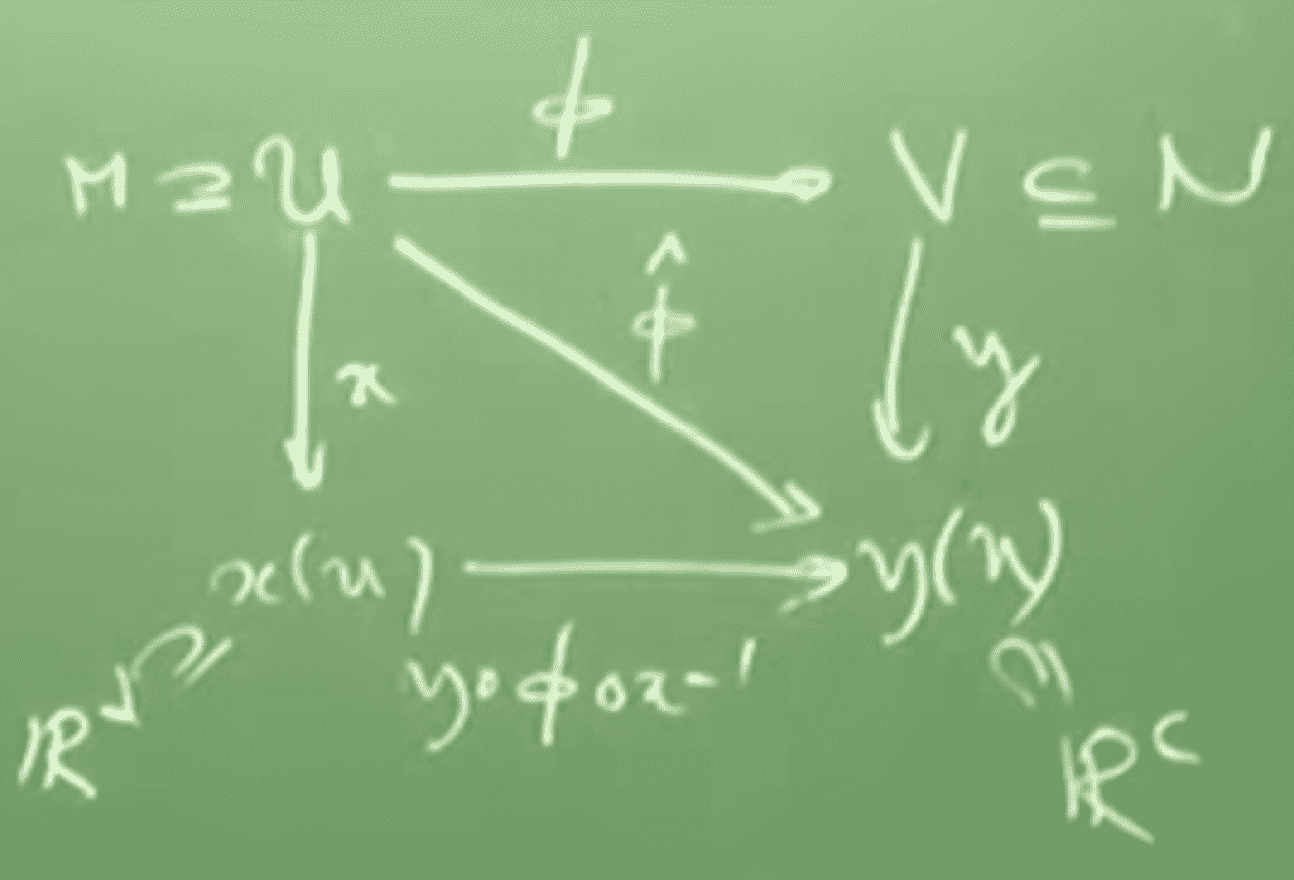
\includegraphics[width=0.3\textwidth]{Figs/4.png}
    % \caption{Extendible and nonextendible vector}
    % \label{fig:trgfdsf}
\end{figure}

The following figure gives a nice pictorial description of the push-froward map.

\begin{figure}[h]
    \begin{center}
        \btik
            \draw[thick] (-3,0) .. controls (-1.7,1.75) .. (-1,3.5);
            \draw[thick] (-1,3.5) .. controls (1.5,3.3) .. (3.5,3.5);
            \draw[thick] (3.5,3.5) .. controls (2.9,1.75) .. (3, 0.3);
            \draw[thick] (-3,0) .. controls (0,0.33) .. (3,0.3);
            \node at (0, 4) {\Huge{$\cM$}};
            %
            \draw[thick] (4.5,0) .. controls (5.3,1) .. (6,3.5);
            \draw[thick] (6,3.5) .. controls (7.5,3.5) .. (10,4);
            \draw[thick] (10,4) .. controls (10,2) ..(10.5,0);
            \draw[thick] (4.5,0) .. controls (7.5,0.2) .. (10.5,0);
            \node at (7, 4) {\Huge{$\cN$}};
            %
            \draw[thick] (-2.3, 0.5) .. controls (-1,1) and (1,3) .. (3,3);
            \node at (-1.9,0.4) {\Large{$\gamma$}};
            \node[circle, fill=black, inner sep=1.25pt] at (0,1.89) {};
            \node at (0,1.5) {\Large{$p$}};
            \draw[->, ultra thick, red] (0,1.89) -- (1,2.6);
            \node at (0.4, 2.7) {\color{red}\Large{$v_{\gamma,p}$}};
            %
            \draw[thick] (6.3,3) .. controls (11.5,3) and (3.5,1) .. (10, 0.5); 
            \node at (9.5,1) {\Large{$(\phi\circ\gamma)$}};
            \node[circle, fill=black, inner sep=1.25pt] at (7.31,1.3) {};
            \node at (6.9,0.75) {\Large{$\phi(p)$}};
            \draw[->, ultra thick, red] (7.31,1.3) -- (7.2,2.5);
            \node at (8.15, 2.22) {\color{red}\Large{$\phi_* (v_{\gamma,p})$}};
            %
            \draw[thick, blue, decoration={markings, mark=at position 0.5 with {\arrow{>}}}, postaction={decorate}] (0,1.89) .. controls (3,2) and (5,0.5) .. (7.31, 1.3);
            \node at (4,1.75) {\color{blue}\Large{$\phi$}};
        \etik
        \caption{Given two smooth manifolds and a smooth map $\phi: \cM \to \cN$, the push forward, $\phi_*$, maps tangent vector, $v_{\gamma,p}$ of curve $\gamma$ at point $p \in \cM$ to  from the corresponding tangent vector, $\phi_* (v_{\gamma,p})$, of curve $(\phi \circ \gamma)$ at point $\phi(p) \in \cN$.}
        \label{fig:PushForward}
    \end{center}
\end{figure}

\bc 
\label{col:Pushforward}
    Looking at \Cref{fig:PushForward}, we see that $\phi_* : v_{\gamma,p} \mapsto v_{(\phi\circ\gamma),\phi(p)}$.
\ec 

\bq 
    Let $f\in C^{\infty}(\cN)$ and let $p\in\cM$ be such that $\gamma(\lambda_0)=p$. Then 
    \begin{align*} 
        \begin{split}
            \phi_*\big(v_{\gamma,p}\big) & := v_{\gamma,p}(f\circ \phi) \\
            & = \big( (f\circ \phi) \circ \gamma\big)'(\lambda_0) \\
            & = \big( f\circ (\phi \circ \gamma)\big)'(\lambda_0) \\
            & = v_{(\phi\circ\gamma),(\phi\circ\gamma)(\lambda_0)} \\
            & = v_{(\phi\circ\gamma),\phi(p)}.
        \end{split}
    \end{align*} 
\eq 

\bex 
    An important/interesting example of use of the push-forward is when $\phi$ is an \textit{embedding} map\footnote{It is important we use an embedding here and not just an \textit{immersion}, which can have self-intersections. If we had self intersections we would not have a unique tangent vector to the mapped curve. For more details on embeddings and immersions, see section 3.6 of Renteln's \textit{Manifolds, Tensors and Forms} textbook.} from a $d$-dimensional manifold to a $(d+1)$-dimensional manifold. 
    
    For obvious pictorial reasons, let $d=1$. If $\gamma:(0,1)\to\cM$ is a curve in this $1$-dimensional manifold, then $v_{\gamma,p}$ is an element of the $1$-dimensional tangent space $T_p\cM$. Let $\phi:\cM\hookrightarrow\cN$ be an embedding of $\cM$ into $\cN$, where $\dim\cN=2$. Then the velocity $v_{(\phi\circ\gamma),\phi(p)}$ is an element of the $2$-dimensional tangent space $T_{\phi(p)}\cN$. This allows us to make a connection between the \textit{intrinsic} vector $v_{\gamma,p}$ and the \textit{extrinsic} vector $v_{(\phi\circ\gamma),\phi(p)}$. 
    
    As an analogy, consider an ant walking along a wire laid down on a table. The vector $v_{\gamma,p}$ would be what the ant (who is oblivious to the higher dimensional space) itself says its velocity is, whereas $v_{(\phi\circ\gamma),\phi(p)}$ is what we (who have a birds eye view of the table) would say the ant's velocity is. 
    
    \begin{center}
        \btik 
            \draw[thick] (-1,0) -- (5,0);
            \draw[ultra thick, blue] (0,0) -- (4,0);
            \draw[ultra thick, ->, red] (1,0) -- (2.5,0) node[label={above:\large $v_{\gamma,p}$}, midway]{};  
            \draw[fill=black] (1,0) circle [radius=0.08cm];
            \node at (1,-0.35) {\large{$p$}};
            \node at (3.8,0.3) {\large{\textcolor{blue}{$\gamma$}}};
            \node at (-1,-0.3) {\large{$\cN=\R$}};
            %
            \draw[thick, blue] (7.5, -1) .. controls (9.5,-0.5) and (10,1.5) .. (12.2,1.5);
            \draw[thick] (7,-1.5) -- (12.5,-1.5) -- (12.5,2) -- (7,2) -- (7,-1.5);
            \draw[ultra thick, red, ->, rotate around={32.5:(8.55,-0.55)}] (8.55,-0.55) -- (10.05,-0.55);
            \draw[fill=black] (8.55,-0.55) circle [radius=0.08];
            \node at (8.7,-1) {\large{$\phi(p)$}};
            \node at (10.25,1.5) {\large{\textcolor{blue}{$\phi\circ\gamma$}}};
            \node at (10.75,0) {\large{\textcolor{red}{$v_{(\phi\circ\gamma),\phi(p)}$}}};
            \node at (8,1.5) {\large{$\cM=\R^2$}};
        \etik 
    \end{center}
\eex

\subsection{Pull-back Map: covectors are pulled back.}

\bd[Pull-back]
    Let $\phi:\cM\to\cN$ be a smooth map between two smooth manifolds. Then we define the \textbf{pull-back map} as $\phi^*:T^*\cN\to T^*\cM$ via 
    \begin{align*} 
        \phi^*(\omega) : X := \omega : \phi_*(X).
    \end{align*} 
    for $\omega\in T^*\cN$ and $X\in T\cM$.
\ed 

Again let's look at the components with respect to the two charts $(U,x)\in\cA_{\cM}$ and $(v,y)\in\cA_{\cN}$.
\begin{align*}
    {\phi^{*\,a}}_i := \phi^*\big((dy^a)_{\phi(p)}\big) : \bigg(\frac{\p}{\p x^i}\bigg)_p = (dy^a)_{\phi(p)} : \phi_*\Bigg(\bigg(\frac{\p}{\p x^i}\bigg)_p\Bigg) =: \phi_{*\,\,i}^{\,\,a},
\end{align*} 
so the \tb{components of the pull-back and the components of the push-forward are the same}!


Just as we showed that the push-forward of a velocity to a curve was the velocity of the mapped curve, the pull-back of the differential of some function is the differential of a function that is mapped to the other function. That is 
\begin{lema}
 \begin{align*} 
    \phi^*(df) = d(f\circ \phi).
\end{align*}
\end{lema}

\begin{proof}
    By definition, we have
\begin{align*}
    (\phi_*X)\la f \ra = X \la f\circ \phi \ra,
\end{align*}
for $X\in T\cM$, giving
\begin{align*}
    \begin{split}
        \phi^*(df) : X & := df : \phi_*(X) \\
        & = \phi_* X \la f \ra \\
        & = X \la f\circ \phi \ra \\
        & = d(f\circ \phi) : X ,
    \end{split}
\end{align*}
which holds for arbitrary $X$ and therefore proves the result. 
\end{proof}

\bd 
    Let $\phi:\cM\to\cN$ be a smooth map between two smooth manifolds. Then the pull back of $f\in C^{\infty}(\cN)$ is given by 
    \begin{align*} 
        \phi^*(f) := f\circ \phi.
    \end{align*} 
\ed 
\bp 
    The pull-back map and the map $d$ commute. That is 
    \begin{align*} 
        \phi^*(d \bullet) = d(\phi^*\bullet).
    \end{align*} 
\ep 
\begin{rema}
 The mnemonic phrase here is \tb{``covectors are pulled back''.}
\end{rema}


\subsection{Induced Metric}

There is an important application for the pull-back. Again consider $\phi:\cM\hookrightarrow\cN$ as an embedding with $\dim\cM <\dim\cN$. Now let the smooth manifold with $\cN$ be equipped with a metric, $g$. We now want to ask whether we can use this metric to define one on the manifold with $\cM$, which we shall call the \textit{induced metric}, $g_{\cM}$. The metric is a $(0,2)$-tensor field, and so can be pulled-back. The question we want to answer is "But how do we define such a metric?"

The way we want this to work is the following. We want to work out the length of a path, $\gamma$, between two points on $\cM$ using $g_{\cM}$. We take the value to be the length of the mapped path, $\phi\circ\gamma$, obtained using $g$. We can write this mathematically as the following definition. 

\bd\bfs{Induced Metric}\label{def:dfafrerq}
    Let $(\cM,\cO,\cA)$ and $(\cN,\cO,\cA)$ be a smooth manifolds, with $|\cM|\leq |\cN|$ and let $\phi:\cM\hookrightarrow\cN$ be an embedding. Now equip $(\cN,\cO,\cA)$ with a metric $g$. We define the \textbf{induced metric} on $\cM$ as the pullback $g_{\cM} := \phi^* g$, which satisfies\footnote{The push-forward of a vector field is simply defined point wise, i.e. push-forward each vector and make a vector field.} 
    \begin{align*} 
        g_{\cM}(X,Y) := g\big(\phi_*(X),\phi_*(Y)\big),
    \end{align*} 
    for all $X,Y\in \Gamma T\cM$. 
\ed 
\begin{rema}
Now obviously there is more then one way to embed the space. Each one of these embeddings gives a potentially different length, and so defines a different metric (and shape) for $(\cM,\cO,\cA)$. We can decide which it is by defining an embedding $\phi:S^2\hookrightarrow\R^3$ such that the induced metric gives the correct shape. This is what our eyes do when differentiating a football from a potato; they look at the lengths between points using our 3D Euclidean metric and conclude that the induced metric is that of a football (or potato). 
\end{rema}

The above condition in the definition can be written in components as 
\begin{align*}
    (g_{\cM})_{ij} = g_{ab} \frac{\p \hat{\phi}^a}{\p x^i}\frac{\p \hat{\phi}^b}{\p x^j},
\end{align*} 
where $\hat{\phi} = (y\circ \phi)$, as in the calculation for the components of the push-forward.

\bex 
    Pictorially we can see the above ideas via the following drawings. Let $(\cM,\cO,\cA)$ be some 2-dimensional smooth manifold and let $(\cN,\cO,\cA,g) = (\R^3,\cO_{st},\cA,g_E)$, the Euclidean $3$-space. We could define an embedding $\phi:\cM\hookrightarrow\R^3$ such that $(\cM,\cO,\cA)$ looks dome shaped w.r.t. the metric $g_E$. We can then pull this metric back onto the $\cM$ manifold itself, giving the induced metric space $(\cM,\cO,\cA,g_{\cM})$.
    \begin{center}
        \btik[scale=0.9]
            \draw[thick, fill = gray!40, opacity = 0.8] (0,0) -- (4,0) -- (4,3) -- (0,3) -- (0,0);
            \draw[ultra thick, blue] (0.5,0.5) .. controls (1.5,2) and (2.5,1) .. (3.5,2.5);
            \node at (2,3.5) {$(\cM,\cO,\cA)$};
            %
            \draw[thick,->] (4.5,1.5) -- (6.5,1.5);
            \node at (5.5,1.9) {\Large{$\phi$}};
            %%
            \node at (9,4) {$(\R^3,\cO_{st},\cA,g_E)$};
            \draw[thick, rotate around={-40:(9,1.5)}] (9,1.2) -- (9,3.5);
            \draw[thick] (9,-0.5) -- (9,2);
            \draw[thick, ->, rotate around={-100:(9,1.5)}] (9,0.7) -- (9,3.5);
            %
            \draw[thick, scale=0.8, fill = gray!40, opacity = 0.8, rotate around={-10:(8.75,1.5)}, yshift = 0.5cm] (8.75,1.5) .. controls (10.25,3.5) and (11.75,3.5) .. (13.25,1.5);
            \draw[thick, scale=0.8, fill = gray!40, opacity = 0.8, rotate around={-10:(8.75,1.5)}, yshift = 0.5cm] (8.75,1.5) arc (180:360: 2.25 and 0.4);
            \draw[dashed, scale=0.8, rotate around={-10:(8.75,1.5)}, yshift = 0.5cm] (13.25,1.5) arc (0:180:2.25 and 0.4);
            %
            \draw[thick, <-, rotate around={-40:(9,1.5)}] (9,-0.5) -- (9,1.2);
            \draw[thick, ->] (9,2) -- (9,3.5);
            \draw[thick, rotate around={-100:(9,1.5)}] (9,-0.5) -- (9,0.7);
            \draw[blue, ultra thick, scale=0.8, rotate around={-10:(8.75,1.5)}, yshift = 0.5cm] (10.25,1.5) .. controls (10.55,1.5) and (10.95,2.5) .. (11.75,2.5);
            %%
            \draw[thick,->] (11.5,1.5) -- (13.5,1.5);
            \node at (12.5,1.9) {\Large{$\phi^*$}};
            %
            \node at (16.25,3) {$(\cM,\cO,\cA,g_{\cM})$};
            \draw[thick, fill = gray!40, opacity = 0.8] (14,1) .. controls (15.5,3) and (17,3) .. (18.5,1);
            \draw[thick, fill = gray!40, opacity = 0.8] (14,1) arc (180:360: 2.25 and 0.4);
            \draw[dashed] (18.5,1) arc (0:180:2.25 and 0.4);
            \draw[blue, ultra thick] (15.5,1) .. controls (15.8,1) and (16.2,2) .. (17,2);
        \etik 
    \end{center}
\eex 

\subsection{Flow of a Complete Vector Field}

\bd[Integral Curve]
    Let $(\cM,\cO,\cA)$ be a smooth manifold and let $\gamma:(a,b)\to \cM$ be a smooth curve with $(a,b)\se\R$. If we have a vector field $X\in\Gamma T\cM$, then $\gamma$ is said to be an \textit{integral curve} of $X$ if
    \begin{align*} 
        v_{\gamma,\gamma(\lambda)} = X_{\gamma(\lambda)}.
    \end{align*} 
    That is, the tangent vectors to the curve reproduce the vector field constrained to the curve. 
\ed 

\bex 
    An example of a integral curve would be that corresponding to a paper ship floating down a river. The vector field $X$ would be the velocity field of the water molecules and the curve $\gamma$ would be the trajectory of the ship. 
\eex 

\bd[Complete Vector Field]
    A vector field $X\in\Gamma T\cM$ is called \textbf{complete} if all integral curves have domain $\R$ (i.e. $(a,b)=\R$).
\ed 

It is tempting to think that this is always possible because you can just reparameterise $\gamma$ such that $(a,b)=\R$, right? Well it's true that you can do this, but in doing so you change the absolute value/length of the tangent vectors and then they no longer coincide with the vector field vectors. So the choice of parameterisation if chosen by the absolute values of the vectors in the vector field. 

Following from the above point, note that for a vector field to be complete it is important that we don't remove points from the domain of the vector field. If we did this, the integral curve through that point would then have finite length and so we would not be able to extend the interval $(a,b)$ to the whole of $\R$ without breaking the integral curve nature. This is a really important point because it leads the way to a proper understanding of singularity\footnote{A singularity can be thought of as a point that is removed from the spacetime because, for example, the curvature blows up there.} theorems.

This result is contained within the following theorem. 

\bt 
    A compactly\footnote{A topological space is said to be compact if every open cover has a finite subcover. For more details see, e.g., Renteln's Manifolds, Tensors, and Forms textbook.} supported, smooth vector field is complete. 
\et 

\begin{figure}[h]
    \begin{center}
        \btik[scale=1.5]
            \draw[ultra thick, red] (-4.1,-0.05) .. controls (-3.32,0.45) .. (-3,0.8) .. controls (-2.6,1.2) .. (-1.7,1.5);
            \node at (-4,1.5) {\Large{$X$}};
            \node at (-1.5, 1.7) {\color{red}\Large{$\gamma$}};
            %
            \draw[thick, blue] (-3.5,-0.8) .. controls (-1,0.6) and (-4,1.5) .. (-2.5,2.5);
            \node at (-2.2,2.5) {\color{blue}\Large{$\sigma$}};
            %
            \draw[->, thick, rotate around={30: (-4,0)}] (-4,0) -- (-3.3,0);
            \draw[->, thick, rotate around={45: (-3,0)}, yshift=0.55cm, xshift=0.3cm] (-3,0) -- (-2.3,0);
            \draw[->, thick, rotate around={20: (-2,0)}, yshift=1.32cm] (-2,0) -- (-1.3,0); 
            %
            \draw[->, thick, rotate around={30: (-3.7,-0.5)}] (-3.7,-0.5) -- (-3,-0.5);
            \draw[->, thick, rotate around={45: (-2.7,-0.5)}, yshift=0.55cm, xshift=0.3cm] (-2.7,-0.5) -- (-2,-0.5);
            \draw[->, thick, rotate around={20: (-1.7,-0.5)}, yshift=1.32cm] (-1.7,-0.5) -- (-1,-0.5);
            %
            \draw[->, thick, rotate around={30: (-4.3,0.5)}] (-4.3,0.5) -- (-3.6,0.5);
            \draw[->, thick, rotate around={45: (-3.3,0.5)}, yshift=0.55cm, xshift=0.3cm] (-3.3,0.5) -- (-2.6,0.5);
            \draw[->, thick, rotate around={20: (-2.3,0.5)}, yshift=1.32cm] (-2.3,0.5) -- (-1.6,0.5);
            %
            \draw[ultra thick, red] (1.5,2) .. controls (2.2,2) .. (2.45,1.5) .. controls (2.8,1) .. (2.45,0.4) .. controls (2.2,-0.2) .. (1.5, -0.2) .. controls (0.9,-0.2) .. (0.65,0.4) .. controls (0.28,0.9) .. (0.65,1.4) .. controls (0.95,2.05) .. (1.5,2);
            \node at (2.5,2.2) {\Large{$Y$}};
            \node at (3,1.5) {\color{red}\Large{$\delta$}};
            %
            \draw[->, thick] (1.05,2) -- (2.05,2);
            \draw[->, thick, rotate around={-60: (2.2,1.9)}] (2.2,1.9) -- (3.2,1.9);
            \draw[->, thick, rotate around={-120:(2.7,0.8)}] (2.7,0.8) -- (3.7,0.8);
            \draw[->, thick] (2,-0.2) -- (1,-0.2);
            \draw[->, thick, rotate around={(-60):(0.9,-0.05)}] (0.9, -0.05) -- (-0.1,-0.05);
            \draw[->, thick, rotate around={60:(0.4,1)}] (0.4, 1) -- (1.4, 1);
            %
            \draw[->, thick] (1.35,1.5) -- (1.85,1.5);
            \draw[->,thick, rotate around={-60:(1.9,1.4)}] (1.9,1.4) -- (2.4,1.4);
            \draw[->,thick,rotate around={-120:(2.15,0.85)}] (2.15,0.85) -- (2.65,0.85);
            \draw[->, thick] (1.85,0.3) -- (1.35,0.3);
            \draw[->,thick, rotate around={-60:(1.3,0.4)}] (1.3,0.4) -- (0.7,0.4);
            \draw[->,thick, rotate around={60:(1,1)}] (1, 1) -- (1.5,1);
        \etik
        \caption{Left: $\gamma$ is an integral curve of the smooth vector field $X$ as its tangent vectors at all points reproduce the vector field at those points. $\sigma$ is not a integral curve as the tangent vectors do not coincide with the vector field vectors at that point. Right: Example of a complete vector field, $Y$. The integral curves, $\delta$, are closed and therefore have domain $\mathbb{R}$. If we were to remove one point in the space, we would not longer have a complete vector field as one of the integral curves would then have finite length.}
    \end{center}
\end{figure}

\bd[Flow of a Complete Vector Field]
    The \textbf{flow of a complete vector field} $X\in\Gamma T\cM$ is a one-parameter family 
    \begin{align*} 
        \begin{split}
            h^X : \R \times \cM & \to \cM \\
            (\lambda, p) & \mapsto \gamma_p(\lambda),
        \end{split}
    \end{align*} 
    where $\gamma_p:\R\to\cM$ is \textit{the} integral curve of $X$ with $\gamma(0)=p$. 
\ed 

We can use the above definition to introduce a new map by simply taking a fixed value for $\lambda$. That is, for fixed $\lambda\in\R$ we have the smooth map 
\begin{align*}
    h^X_{\lambda} :\cM \to \cM,
\end{align*}  
which takes every point in $\cM$ and moves it a parameter distance $\lambda$ along the integral curve through that point. 

\subsection{Lie Subalgebras of the Lie Algebra $(\Gamma T\cM,[\cdot,\cdot])$ of Vector Fields}

\bd[Lie Algebra]
    A \textbf{Lie algebra} is a vector space\footnote{In fact you only need a module over a commutative ring.} $\mathfrak{g}$ equipped with a bilinear operation $[\cdot,\cdot]:\mathfrak{g}\times\mathfrak{g}\to\mathfrak{g}$, known as the \textbf{Lie bracket}, that also satisfies
    \benr 
        \item Antisymmetry: $[x,y]=-[y,x]$, 
        \item The \textit{Jacobi identity}: $\big[x,[y,z]\big] + \big[z,[x,y]\big] + \big[y,[z,x]\big]= 0$
    \een 
\ed 

\bd[Structure Constants]
    Let $(\mathfrak{g},[\cdot,\cdot])$ be a Lie algebra. We define the \textbf{structure constants} of the Lie algebra, ${C^k}_{ij}\in\F$, via 
    \begin{align*} 
        [x_i,x_j] = {C^k}_{ij}x_k
    \end{align*} 
    for $x_i\in\mathfrak{g}$ and $i,j,k\in\{1,...,\dim\mathfrak{g}\}$.
\ed 

Recall in lecture 8 we defined the commutator of two vector fields as 
\begin{align*} 
    [X,Y]\la f \ra = X\big\la Y\la f\ra \big\ra - Y\big\la X\la f\ra \big\ra. 
\end{align*} 
We want to make this into a Lie bracket, however we have to address a problem. As it stands we are considering the $C^{\infty}$-module $(\Gamma T\cM,\oplus,\odot)$, but our commutator does not obey $C^{\infty}$-bilinearity. That is 
\begin{align*} 
    [f\odot X,Y] \neq f\odot [X,Y].
\end{align*} 
However, it does obey $\R$-bilinearity. 

\bp 
\label{prop:LieAlgebraVectorFields}
    If we therefore restrict ourselves to the $\R$-vector space $(\Gamma T\cM,+,\cdot)$ then the commutator becomes a Lie bracket. 
\ep 

\bnn 
    We will denote the Lie algebra of vector fields as just $(\Gamma T\cM,[\cdot,\cdot])$, but it is important to remember that we are considering the restricted to case of $\cdot:\R\times\Gamma T\cM \to \Gamma T\cM$, i.e. $\R$-vector space.
\enn 

\bbox 
    \ben[label=(\alph*)]
    \item Show the above inequality, $[f\odot X,Y] \neq f\odot [X,Y]$.
    \item Prove \Cref{prop:LieAlgebraVectorFields}.
    \een 
\ebox 

\bd[Lie Subalgebra]
    Let $(\mathfrak{g}, [\cdot,\cdot])$ be a Lie algebra. A vector subspace $\mathfrak{a}\se\mathfrak{g}$ is called a \textbf{Lie subalgebra} if it is closed under the Lie bracket. That is, $[x,y]\in\mathfrak{a}$ for all $x,y\in\mathfrak{a}$. 
\ed 

By restricting to $\R$-linearity we get an infinite dimensional vector space. This just comes from the fact that we can only scale the basis vector fields by the same amount at each point (as opposed to with $C^{\infty}$-linearity), and so we need an infinite number of them to have a complete basis. However, we can just restrict ourselves to a subalgebra $(\Span_\R\{X_1,...,X_s\},[\cdot,\cdot])$ of finite dimension. 

\bex 
    An example of such a Lie subalgebra on $(S^2,\cO,\cA)$ is\footnote{We're actually being a bit clumsy here. $\mathfrak{so}(3)$ is the Lie algebra of the Lie group $SO(3)$, which is a manifold equipped with a group structure.}
    \begin{align*} 
        \mathfrak{so}(3) := (\Span_{\R}\{X_1,X_2,X_3\}, [\cdot,\cdot]),
    \end{align*}
    where 
    \begin{align*} 
        [X_1,X_2] = X_3, \qquad [X_3,X_1] = X_2 \qand [X_2,X_3] = X_1.
    \end{align*} 
    This is the 3-dimensional rotation Lie algebra, and finds important use in quantum mechanics.\footnote{For more details see Dr. Schuller's Lectures on Quantum Theory course.}
\eex 

\br 
    In the tutorials we show that 
    \begin{align*} 
        \begin{split}
            X_1(p) & = -\sin\big(\varphi(p)\big) \frac{\p}{\p \theta} - \cot\big(\theta(p)\big)\cos\big(\varphi(p)\big)\frac{\p}{\p \varphi}, \\
            X_2(p) & = \cos\big(\varphi(p)\big) \frac{\p}{\p \theta} - \cot\big(\theta(p)\big)\sin\big(\varphi(p)\big) \frac{\p}{\p \varphi}, \\
             X_3(p) & = \frac{\p}{\p \varphi},
        \end{split}
    \end{align*} 
    is of the form above, justifying why it is often called the 3-dimensional rotation algebra. 
\er 

Note that we can made no reference to a metric at any point here, and so any $\{X_1,X_2,X_3\}$ that satisfies the above will hold on both the round sphere of radius $R$ and on the potato. 

\subsection{Symmetry}

\bd[Symmetry of a Metric]
    Let $(\cM,\cO,\cA,g)$ be a metric manifold, and let $\{X_1,..,X_s\} \ss \Gamma T\cM$. Define $L := \Span_{\R}\{X_1,...,X_s\}$, then the $s$-dimensional Lie subalgebra $(L,[\cdot,\cdot])$ is said to be a \textbf{symmetry} of a metric tensor field $g$, if for all $X\in L$
    \begin{align*} 
        g\big( (h^X_{\lambda})_*(A), (h^X_{\lambda})_*(B)\big) = g(A,B),
    \end{align*}
    for $A,B\in T_p\cM$ and $(h^X_{\lambda})_*$ is the push-forward of the flow of $X$. We can write this alternatively as 
    \begin{align*} 
        (h_{\lambda}^X)^*g = g,
    \end{align*} 
    where $(h_{\lambda}^X)^*$ is the pull-back associated to the flow of $X$.
\ed 

The first part in the above definition basically says that the angle and projection between $A$ and $B$ (which the metric tells you) does not change if you move both $A$ and $B$ along the integral curves of $X$. For example, for the round sphere of radius $R$, if we move $A$ and $B$ around the sphere in the `$\theta$'-direction then obviously nothing changes. 

The second part just says if we move the metric `backwards' along the integral curves, it still looks the same. This is again intuitively clear for a round sphere when we rotate the sphere. It is not true, however, for the potato, because by moving the metric, the shape of the potato moves. This is clearly just the statement that the round sphere is rotationally symmetric, but the potato is not. 

\subsection{Lie Derivatives}\label{sub:inbdarqr}

The above test for symmetry is very intuitive but it has the major flaw that you have to do a lot of calculation. We therefore typically don't use that method, but instead use the following one. 

It follows from the above that if, for all $X\in L$, 
\begin{align*} 
    \lim_{\lambda\to0}\frac{\big(h^X_{\lambda}\big)^*g-g}{\lambda} =0
\end{align*} 
holds then $L$ is a symmetry of $g$. We actually give the left-hand side its own notation. We define the \textit{Lie derivative} of a metric $g$, w.r.t. a vector field $X$ as 
\begin{align*} 
    \cL_Xg := \lim_{\lambda\to0}\frac{\big(h^X_{\lambda}\big)^*g-g}{\lambda}.
\end{align*}

The Lie derivative is actually quite a subtle thing to define. The definition we've used above makes contact with the pull back ideas we discussed above and so we can think of it as comparing the `dragged back'\footnote{Dragged back as the map $h$ is an automorphism, so the pull-back just drags the points backwards.} tensor to the tensor as it is. For another explanation of this see \href{http://web.math.ucsb.edu/~ebrahim/liederivs_tame.pdf}{these notes}.

\br 
    Alternatively, one can define the Lie derivative using \textit{Cartan's formula}. This useful when discussing the Lie derivative of differential forms. We shall not discuss this further her, but for the interested reader the formula is $\cL_X := d\iota_X - \iota_Xd$.\footnote{$d$ is the exterior derivative, which we have touched on in these notes, and $\iota_X$ is the so-called interior derivative w.r.t. $X$.}
\er

Given the above comments, we actually define the Lie derivative in a rather abstract way, but that looks very similar to the definition of the covariant derivative. 

\bd[Lie Derivative]
    The \textit{Lie derivative} $\cL$ on a smooth manifold $(\cM,\cO,\cA)$ sends a pair of a vector \textit{field}, $X$, and a $(p,q)$-tensor \textit{field}, $T$, to a $(p,q)$-tensor field such that: for $f\in C^{\infty}(\cM)$ and $Y\in\Gamma T\cM$,
    \benr 
        \item $\cL_X f= X\la f\ra$, 
        \item $\cL_XY = [X,Y]$,
        \item $\cL_X(T+S) = \cL_XT+\cL_XS$,
        \item $\cL_X\big(T(\omega,Y)\big) = (\cL_XT)(\omega,Y) + T\big(\cL_X\omega,T\big)+T\big(\omega,\cL_XY\big)$ and similarly for different rank tensors,
        \item $\cL_{X+Y}T = \cL_XT + \cL_YT$.
    \een 
\ed 

These conditions look very similar to those of the covariant derivative, but with the Lie derivative we don't need to provide any extra structure, i.e. don't need to define any $\Gamma$s. You might think that this makes the Lie derivative a more useful derivative, however it comes with its own flaws. 

The first thing we notice is that the lower entry for the Lie derivative must be a vector \textit{field}. This is different to the covariant derivative, where we can take just a vector here. This comes from the idea that we need to obtain this flow of $X$, and that clearly involves knowing $X$ in a neighbourhood of the point and so it must be a field. Next we notice that condition (ii) is something not present in the definition of a covariant derivative. It has the drastic effect on condition (v) whereby the Lie derivative is \textbf{not} $C^{\infty}$-linear in the lower slot (as the covariant derivative is). This comes simply from 
\begin{align*} 
    \cL_{fX}Y = [fX,Y] = f[X,Y] - Y\la f \ra X.
\end{align*} 

\bbox 
    There is another important difference to note. Recall that for the components of the covariant derivative of a tensor, each upper index came with a $+$ sign and each lower index came with a $-$ sign. The opposite is true for the Lie derivative. That is, 
    \begin{align*} 
        {(\cL_XT)^i}_j = X^m \frac{\p {T^i}_j}{\p x^m} - \frac{\p X^i}{\p x^m} {T^m}_j + \frac{\p X^m}{\p x^j}{T^i}_m.
    \end{align*} 
    Show that this result holds.
\ebox 

Using the relation in the above exercise, the condition $\cL_Xg=0$ becomes a very easy thing to solve, and so we obtain a nice way to see if a metric features a symmetry. 

\subsection{Killing Vector Fields}

\bd[Killing Vector Field] 
    Let $(\cM,\cO,\cA,g)$ be a metric manifold. A vector field $K\in\Gamma T\cM$ is called a \textbf{Killing vector field} (or just Killing field) if it is a symmetry of the metric, i.e. $\cL_Kg = 0$, which can equally be written as 
    \begin{align*} 
        K\big\la g(X,Y)\big\ra - g\big([K,X],Y\big) - g\big(X,[K,Y]\big) = 0.
    \end{align*} 
\ed 

Noether's theorem tells us that there is a link between symmetries and conservation laws, and so we see that Killing vector fields correspond to conservation laws. For example, as we will see later, the vector field which corresponds to temporal translation $\p_0$ is a Killing vector field Minkowski spacetime, and gives rise to conservation of energy. Similarly we have Killing vector fields for momentum conservation. 

\bbox 
    Show that for the Levi-Civita connection the Killing vector field condition becomes 
    \begin{align*} 
        g\big(\nabla_XK,Y\big) + g\big(X,\nabla_YK\big) = 0.
    \end{align*} 
    \textit{Hint: You need to use both the metric compatible and the Torsion free conditions.}
\ebox 


\section{More Explanation}
In this section, I add more explanation of some abstract concepts that lack of explanations
\subsection{Torsion and Lie Bracket}
\begin{enumerate}[label=\textbf{\arabic*})]
    \item  \tb{Lie commutator:} The Lie commutator $[\cdot,\cdot]$ tell us the difference between $X$ take derivative along $Y$ (view it as a curve) and $Y$ take derivative along $X$. Note it \tb{does not} depends on the connection. However, we \tb{cannot} define it at a specific point. This can be seen if you try to expand it using the local chart representation and note we will need to calculate $\partial_x f$ (which is well defined using the \tb{neighbour} \href{https://math.stackexchange.com/questions/2705586/composition-of-vector-field-regarded-as-sections-of-tangent-bundle}{(See the link)}).
    See Lie Derivatives in \cref{sub:inbdarqr} and \cref{fig:dfadf} for more details.
    \begin{figure}[h]
    \centering
    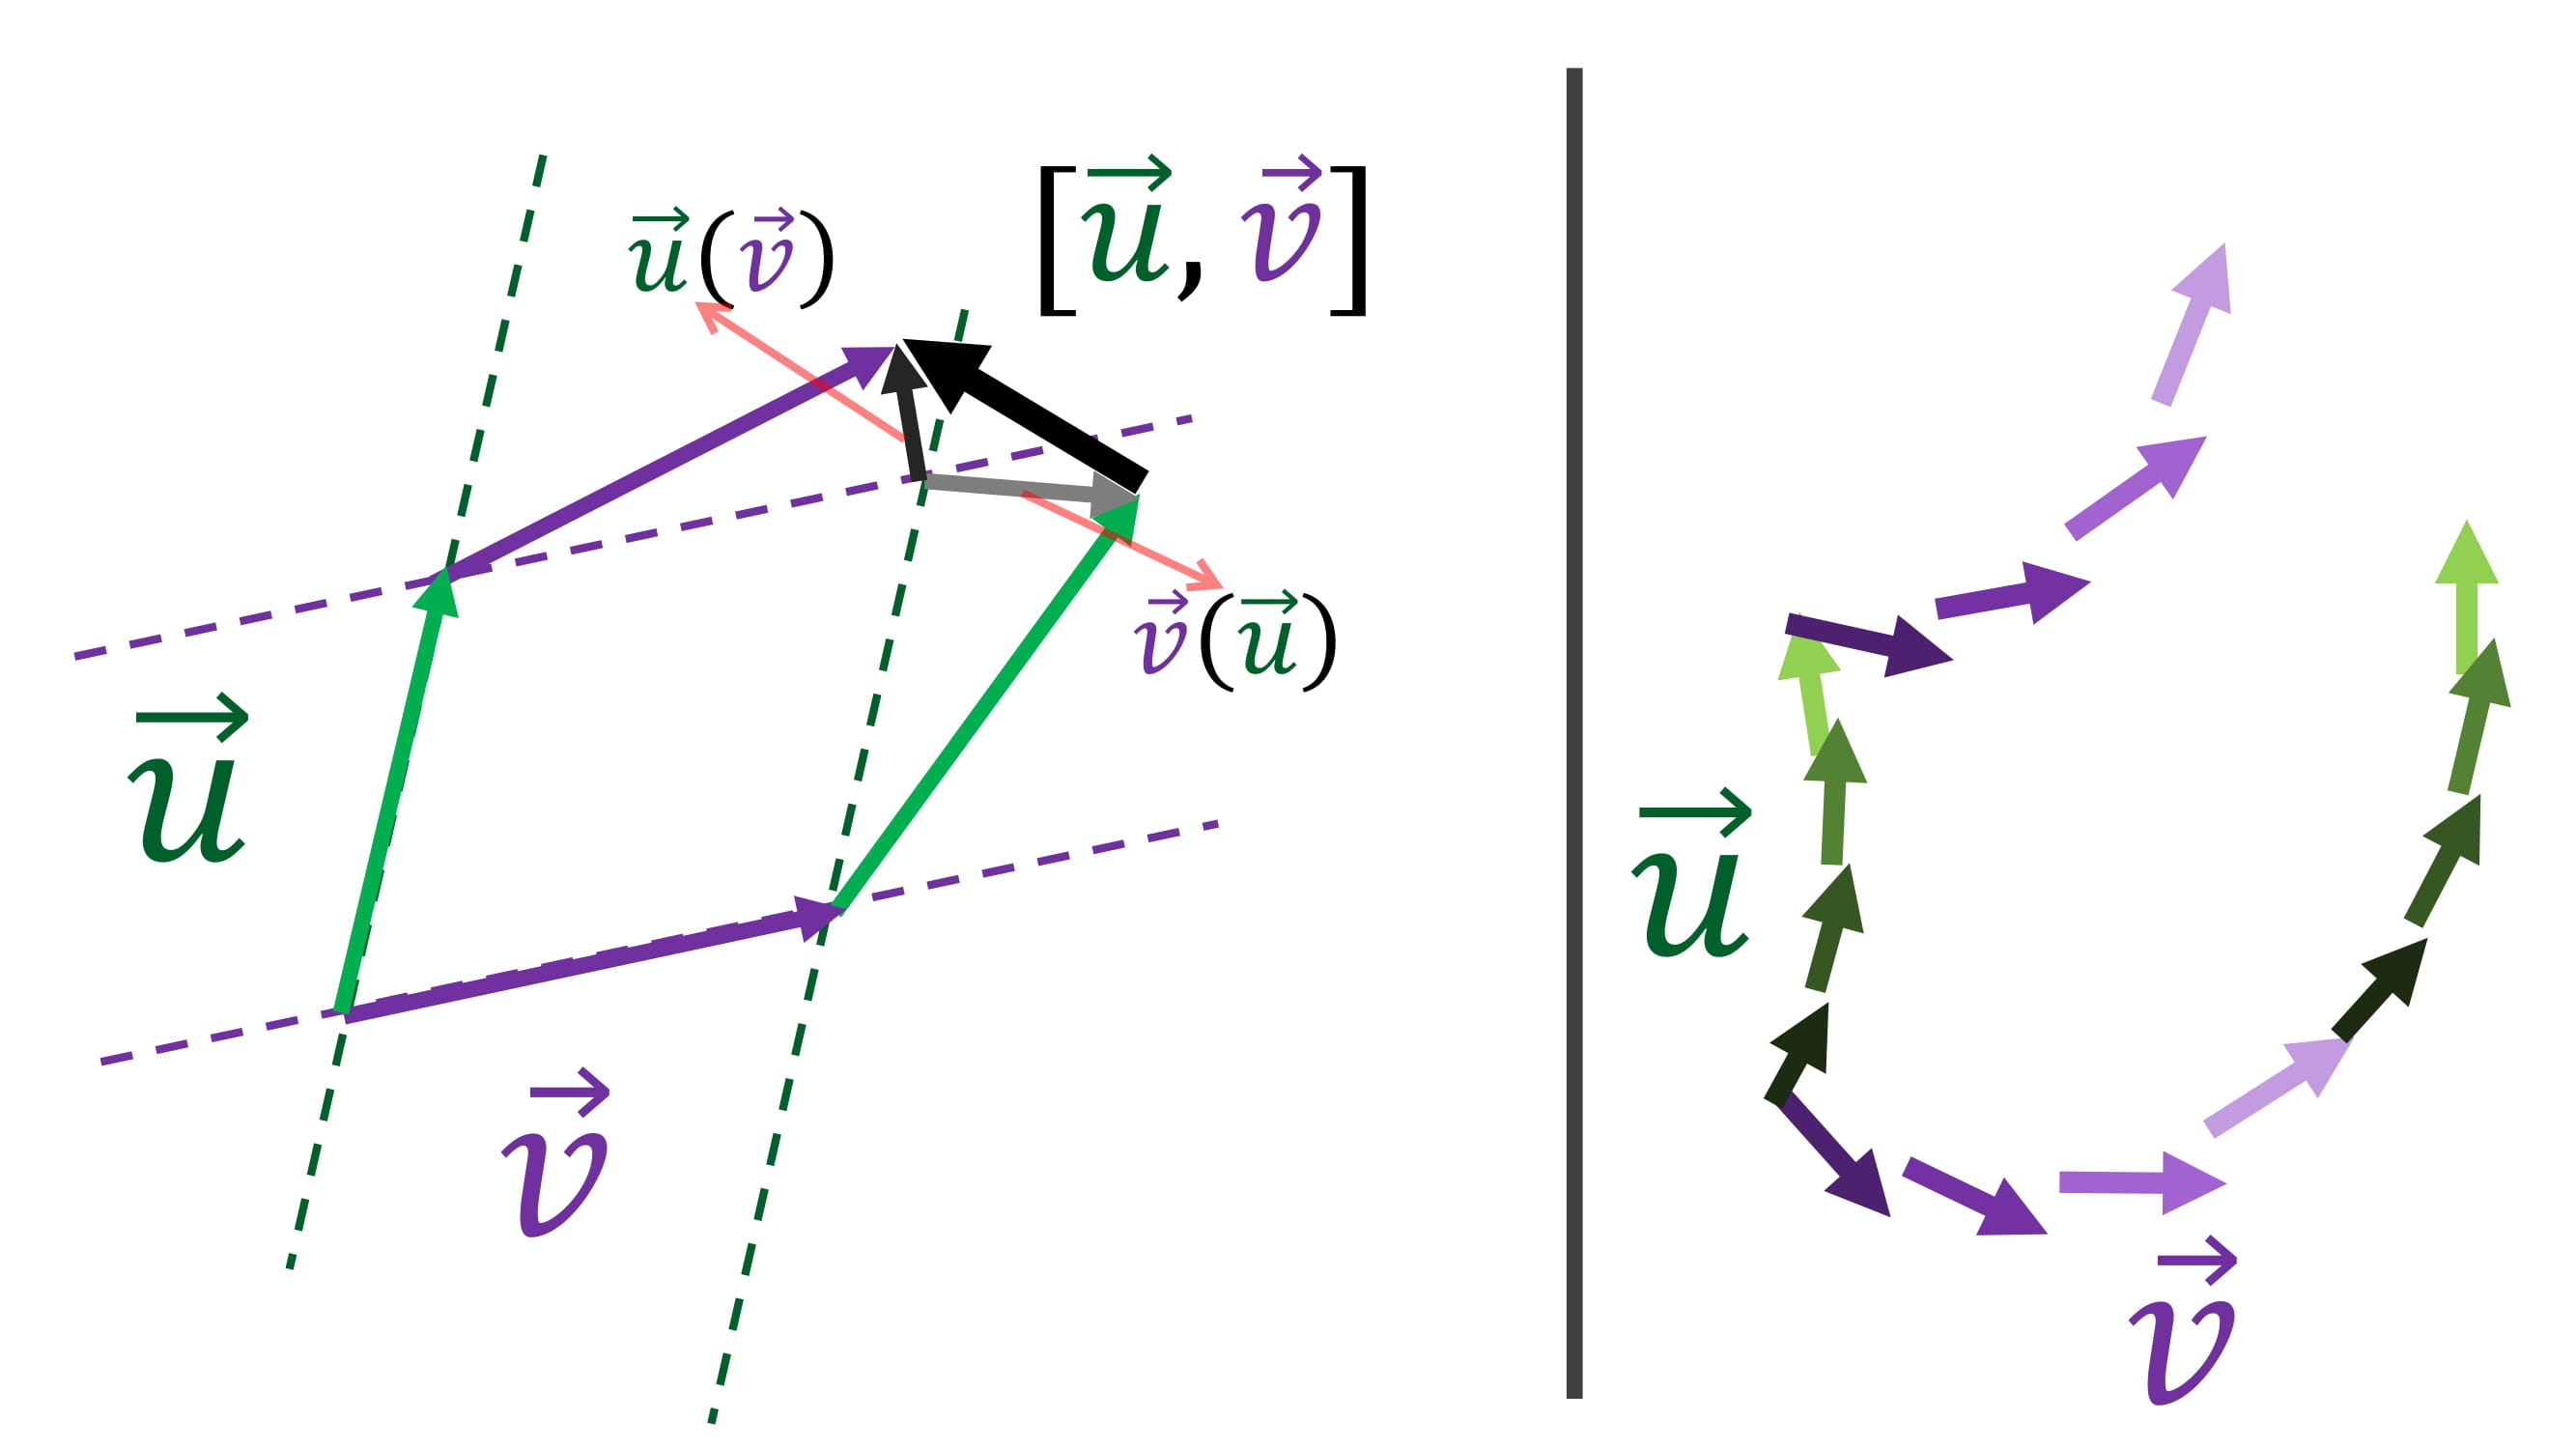
\includegraphics[width=0.7\textwidth]{Figs/e1.jpg}
    \caption{\small Left: local infinite small neighbor. The solid line is the real local vector field while the dash line is the $\vec{u}(\vec{\tilde{v}})=0$ or  $\vec{v}(\vec{\tilde{u}})=0$ for some virtual $\tilde{v}$ or $\tilde{u}$ (more strictly speaking, it does not need both of them $=0$, we only need it to be a closed rectangle, i.e., a grid); Right: global vector field.}
    \label{fig:dfadf}
\end{figure}
    \begin{itemize}
        \item For any \tb{chart induced coordinate map}, we have $[(\frac{\p}{\p x^i}),\frac{\p}{\p x^j}]$, so they form a
grid and must close. See also \cref{re:iqnne}.
 
    \end{itemize}
\item \tb{Torsion:} Here we just take into consideration $ \nabla_XY - \nabla_YX - [X,Y]$.  Note unlike the $ X\big\la Y\la f\ra \big\ra$, $\nabla_XY$ measures how much the difference of $Y$ at each point is away from the vector field by letting $Y_p$ to parallel transport among the $X$ direction. See \cref{fig:oenfndadg} for more details.
    \begin{figure}[H]
    \centering
    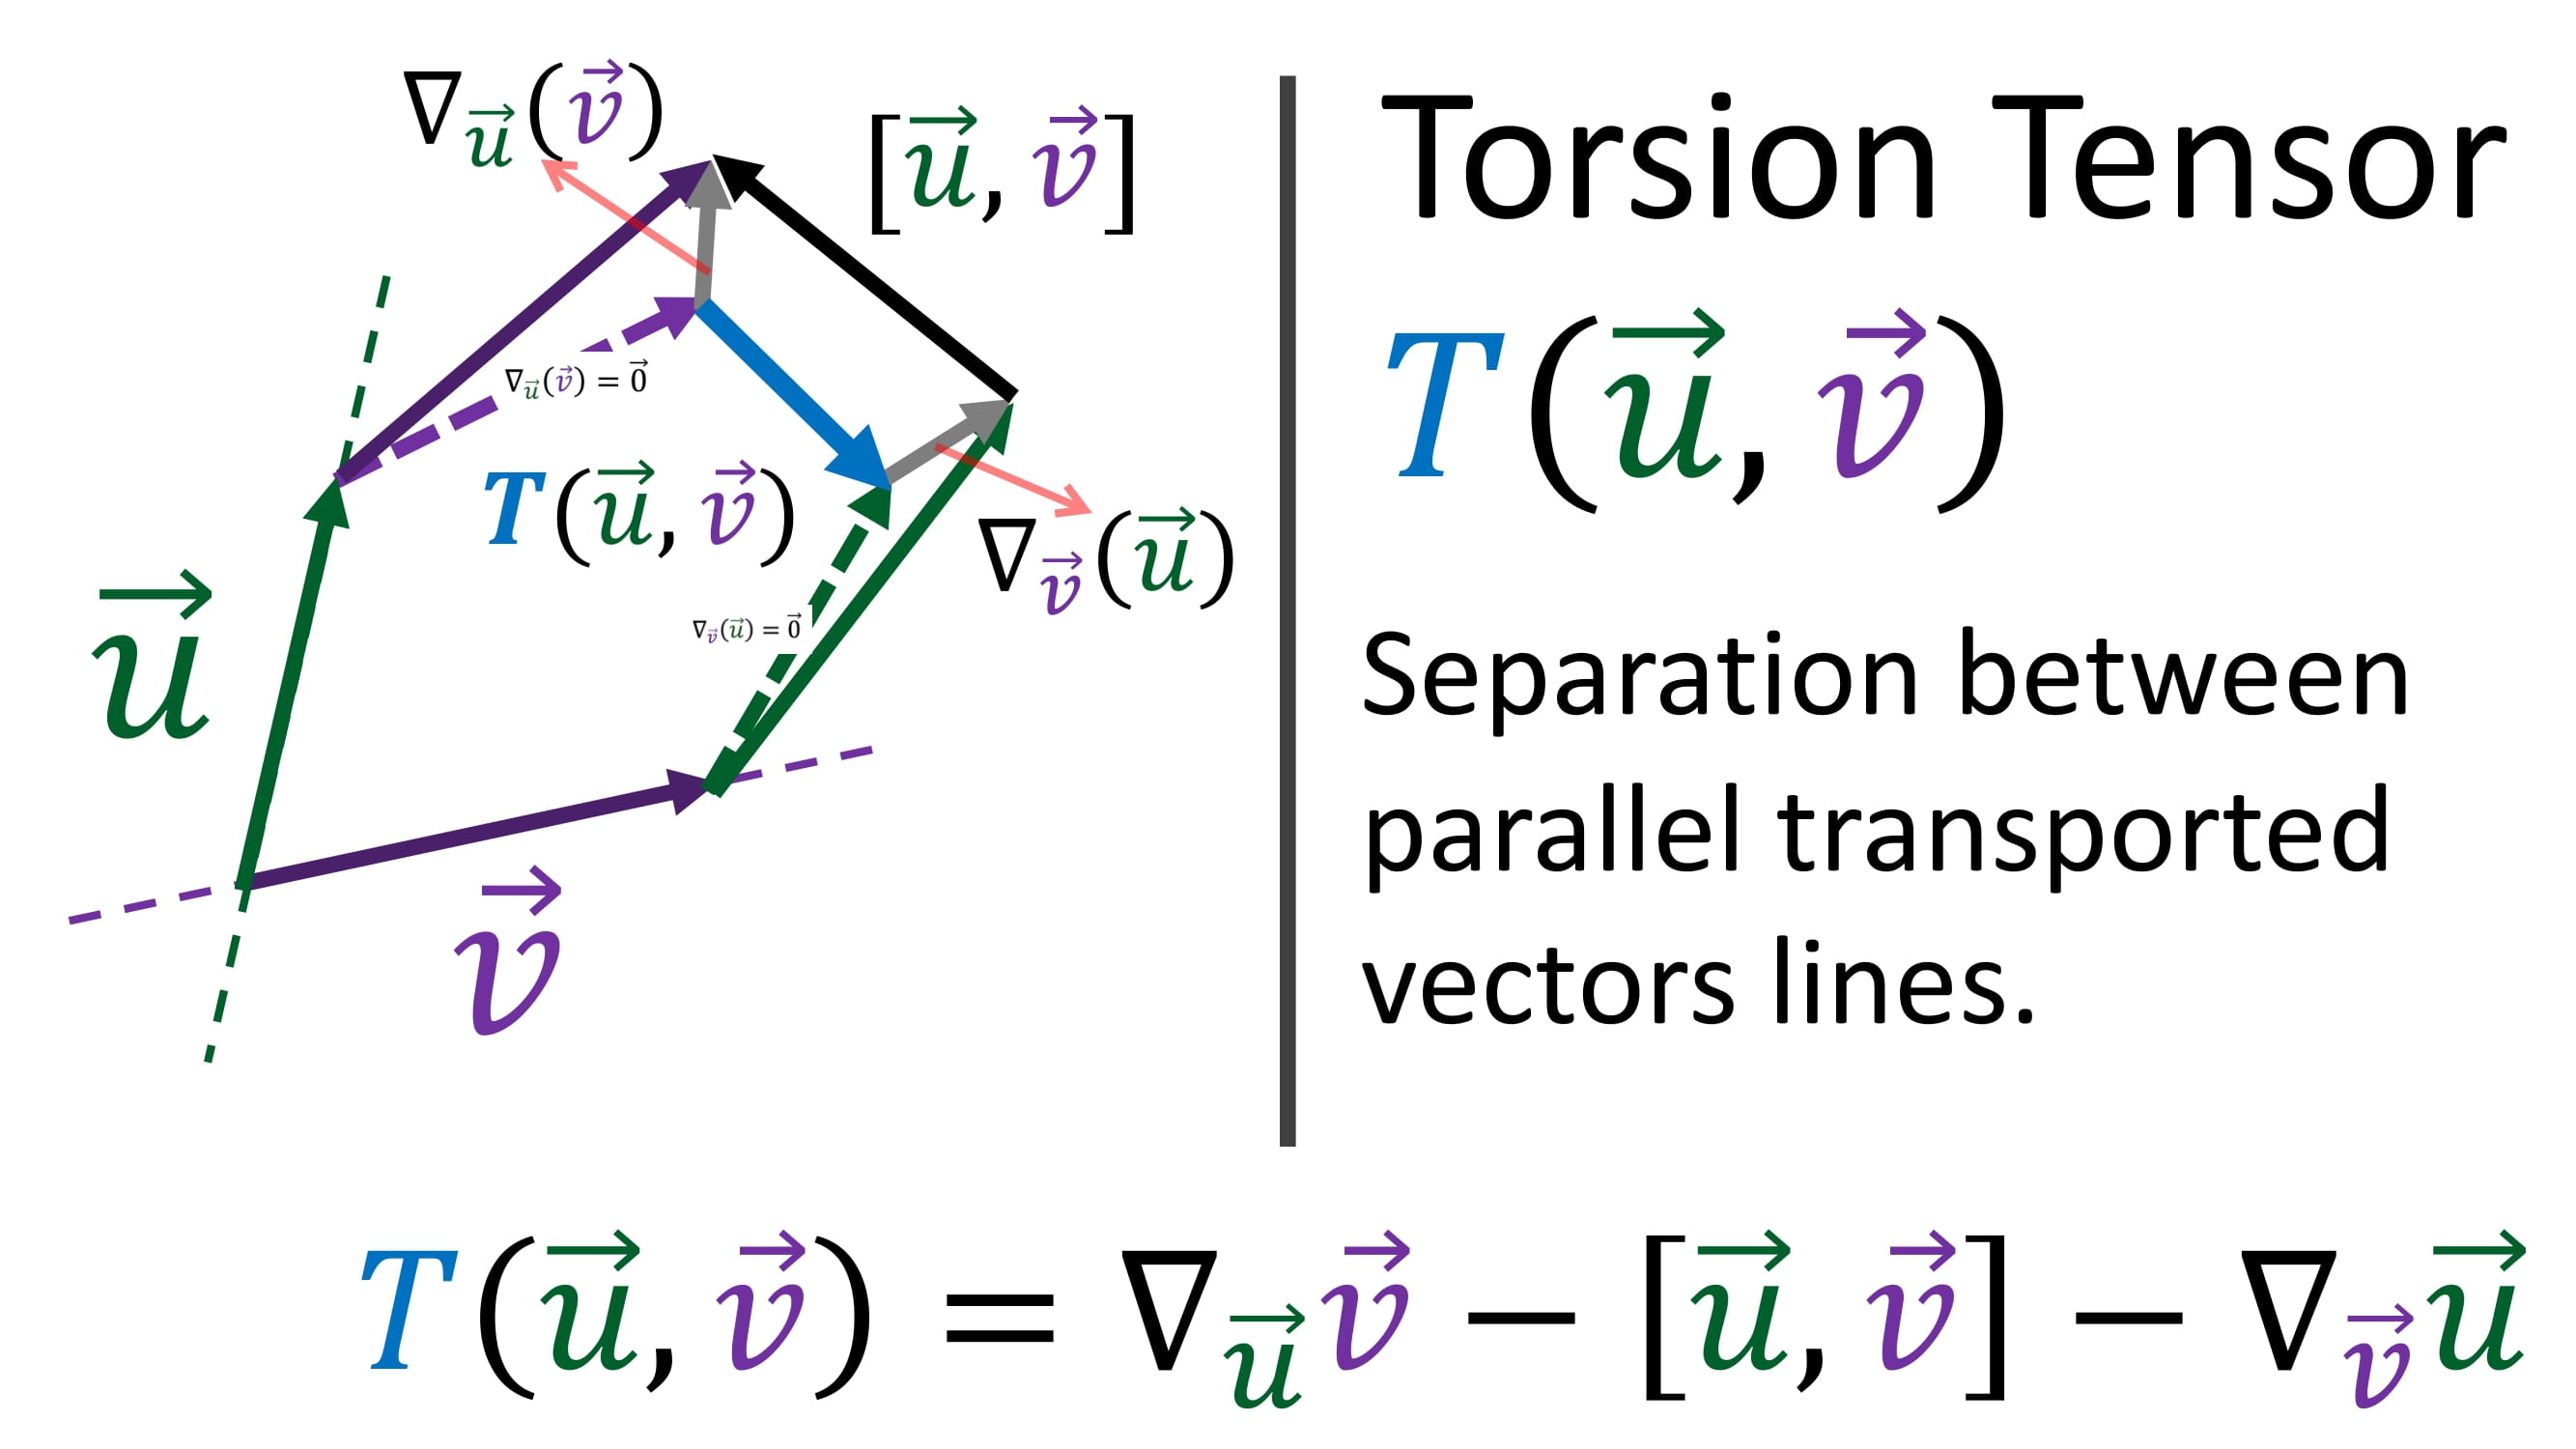
\includegraphics[width=0.7\textwidth]{Figs/e3.jpg}
    \caption{\small local infinite small neighbor: the solid line is the real local vector field while the dash vector is the \tb{parallel transport} along the direction of $\vec{u}$ from $v$ or along the direction of $\vec{v}$ from $u$}
    \label{fig:oenfndadg}
\end{figure}

\item \tb{Torsion Free Connection:} $\nabla_XY - \nabla_YX = [X,Y]$ \tb{for all} $X,Y\in\Gamma T\cM$.  It means the parallel transported vectors close properly. Note, torsion free is a \tb{property of a connection} and it does not depend on the vector field that we use (note the ``for all'')! Torsion free connection only have \tb{symmetric parts}. See \cref{lem:oenqrgrgd} and \cref{fig:dfadgiqdnfnqdd3q} for more details.
    \begin{figure}[H]
    \centering
    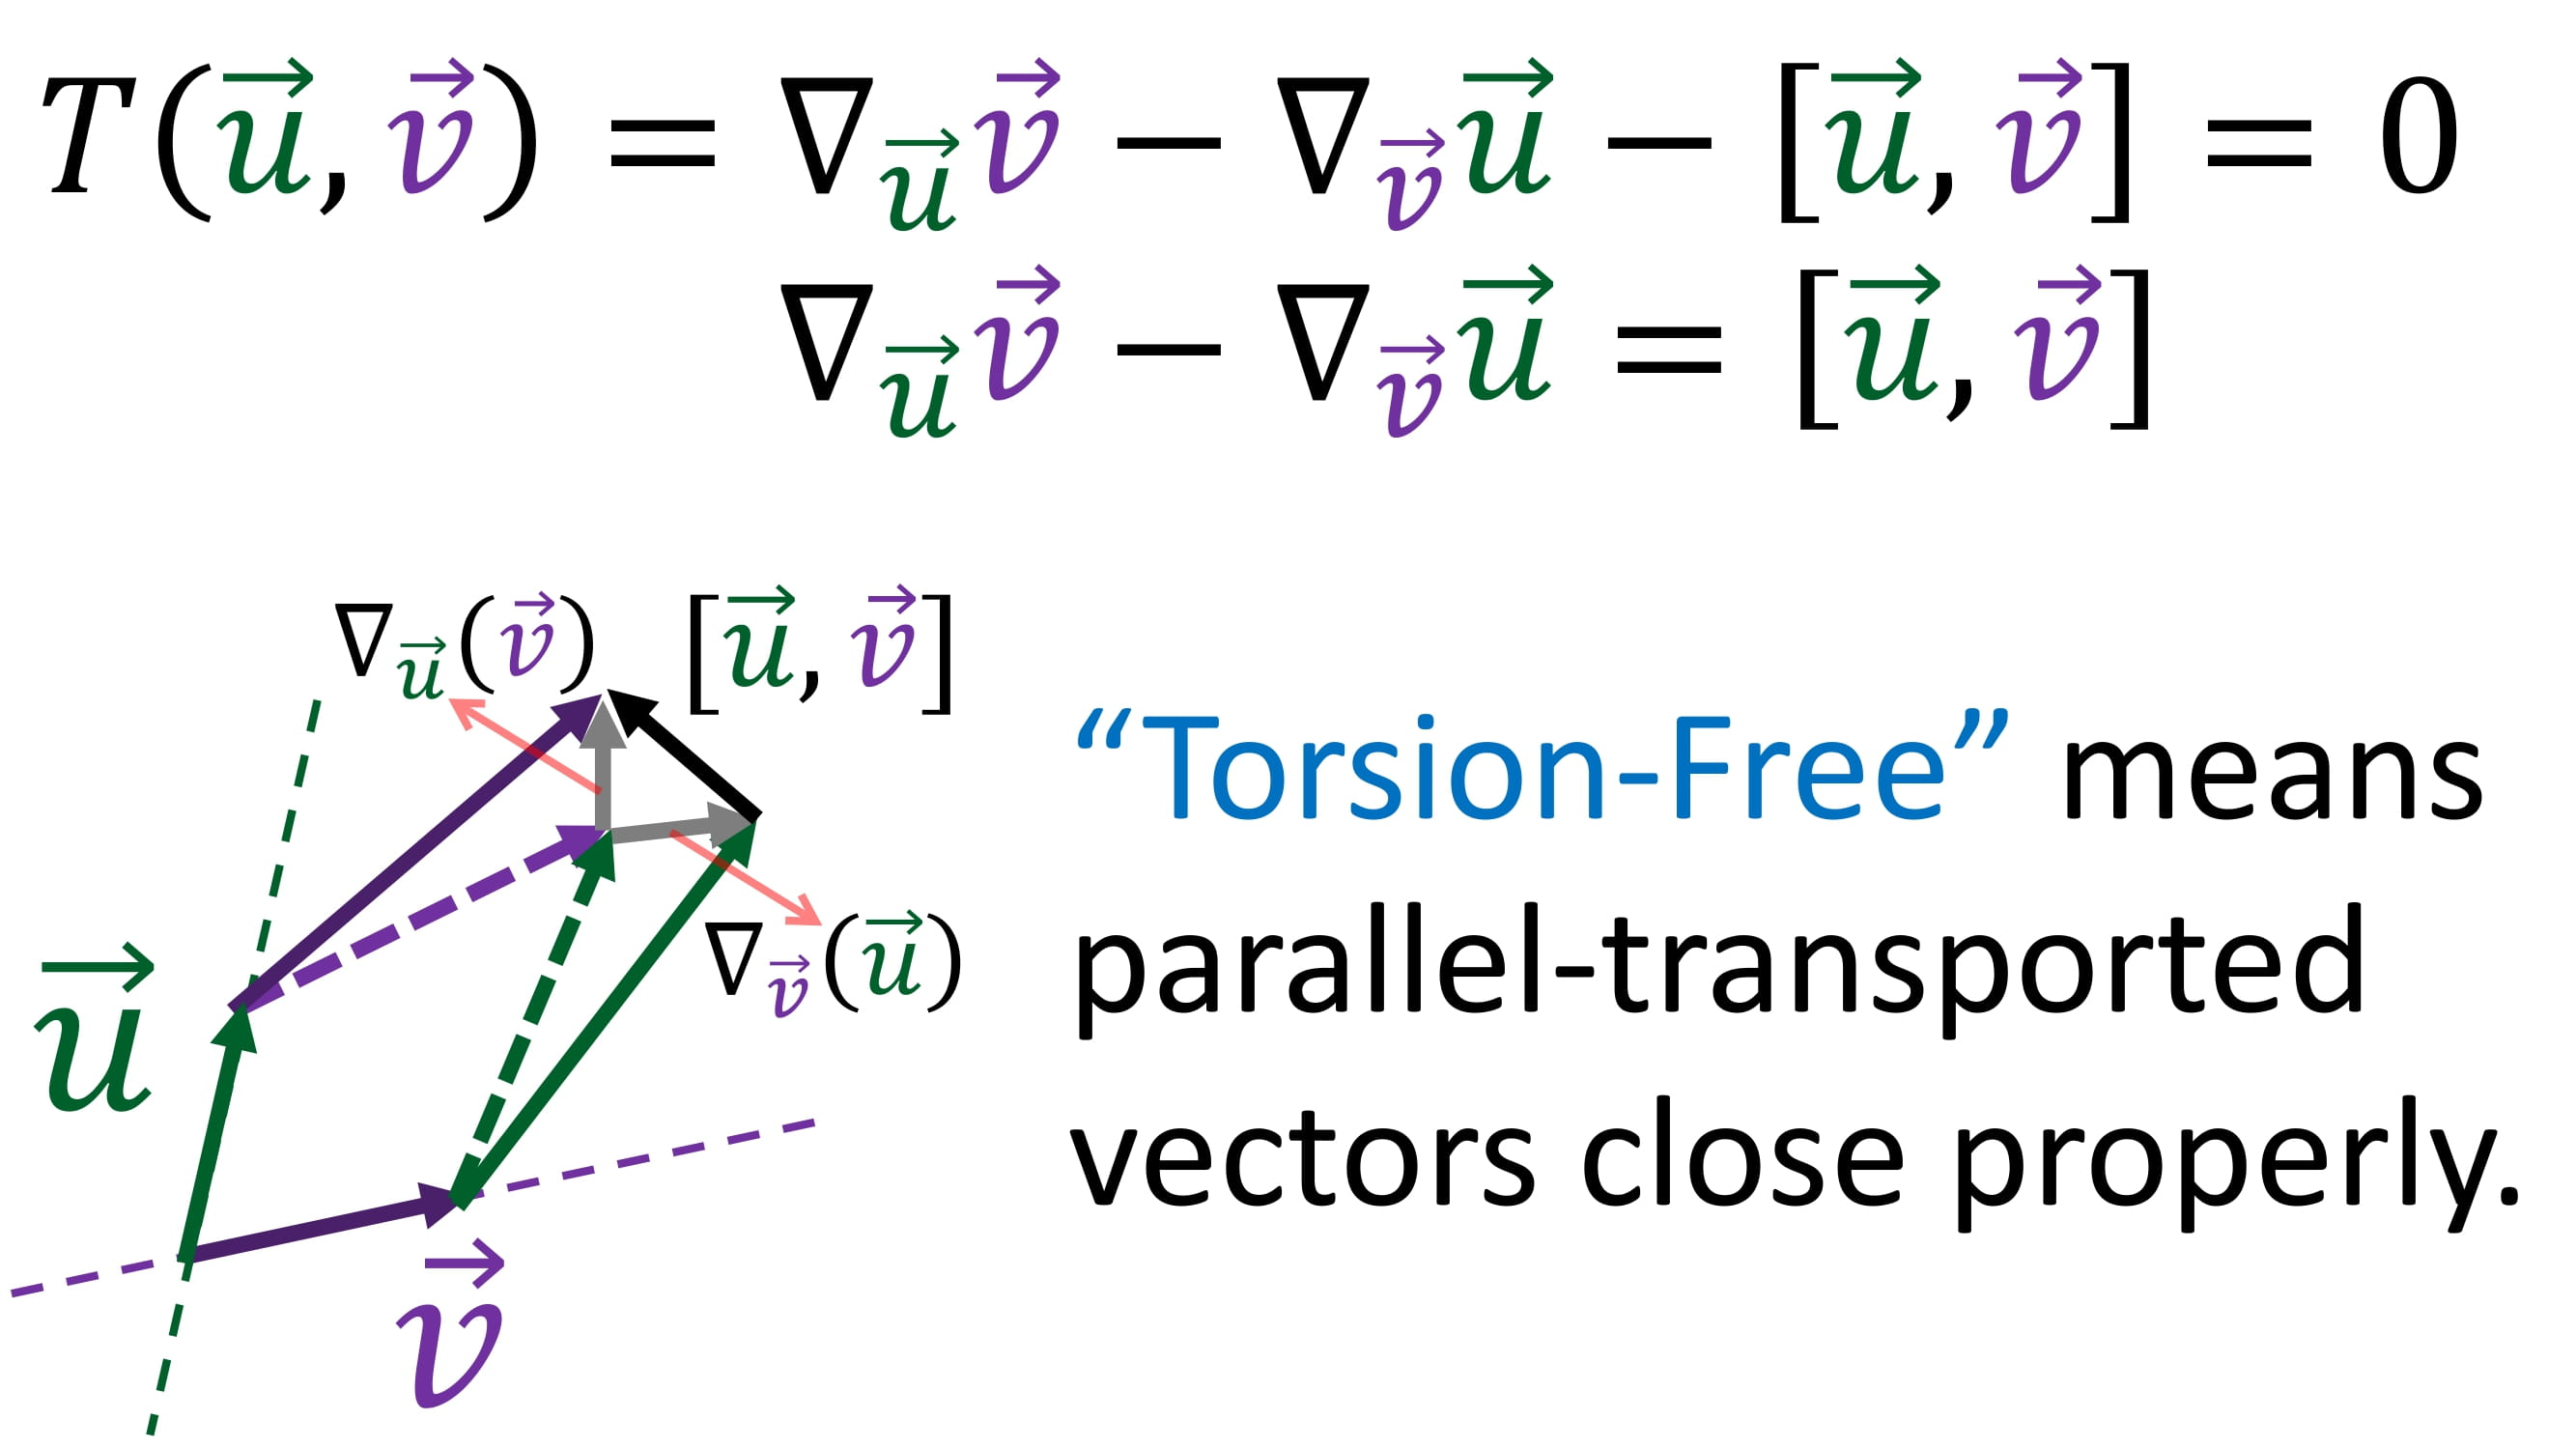
\includegraphics[width=0.7\textwidth]{Figs/e4.jpg}
    \caption{\small Torsion free}
    \label{fig:dfadgiqdnfnqdd3q}
\end{figure}
\end{enumerate}

\subsection{Curvature}
\begin{enumerate}[label=\textbf{\arabic*})]
    \item \tb{Riemann Curvature}: It assigns a tensor to each point of a Riemannian manifold (i.e., it is a tensor field). It is a local invariant of Riemannian metrics which measures the \tb{failure of the second covariant derivatives to commute}. A Riemannian manifold has zero curvature if and only if it is flat, i.e. locally isometric to the Euclidean space. (The curvature tensor can also be defined for any pseudo-Riemannian manifold, or indeed any manifold equipped with a (affine) connection.) We have two explanations:
    \begin{enumerate}[label=(\textbf{\alph*})]
        \item \tb{Holonomy:} See \cref{fig:gadfadf}.  We transport $\vec{w}$ parallelly  around a infinite-small rectangle (if assume Lie bracket is 0). The difference before and after the transport measures how much the space is curved. 
        \begin{itemize}
            \item \tb{Why need the last term?} If Lie bracket is not 0, we need the last term to make it indeed a tensor (i.e., satisfying the multi-linear property). Another interpretation is we transport $\vec{w}$ parallelly now along the (outer) pentagon shown in \cref{fig:dfadf} and calculate the difference before and after the transport.
       \end{itemize}
            \begin{figure}[H]
    \centering
    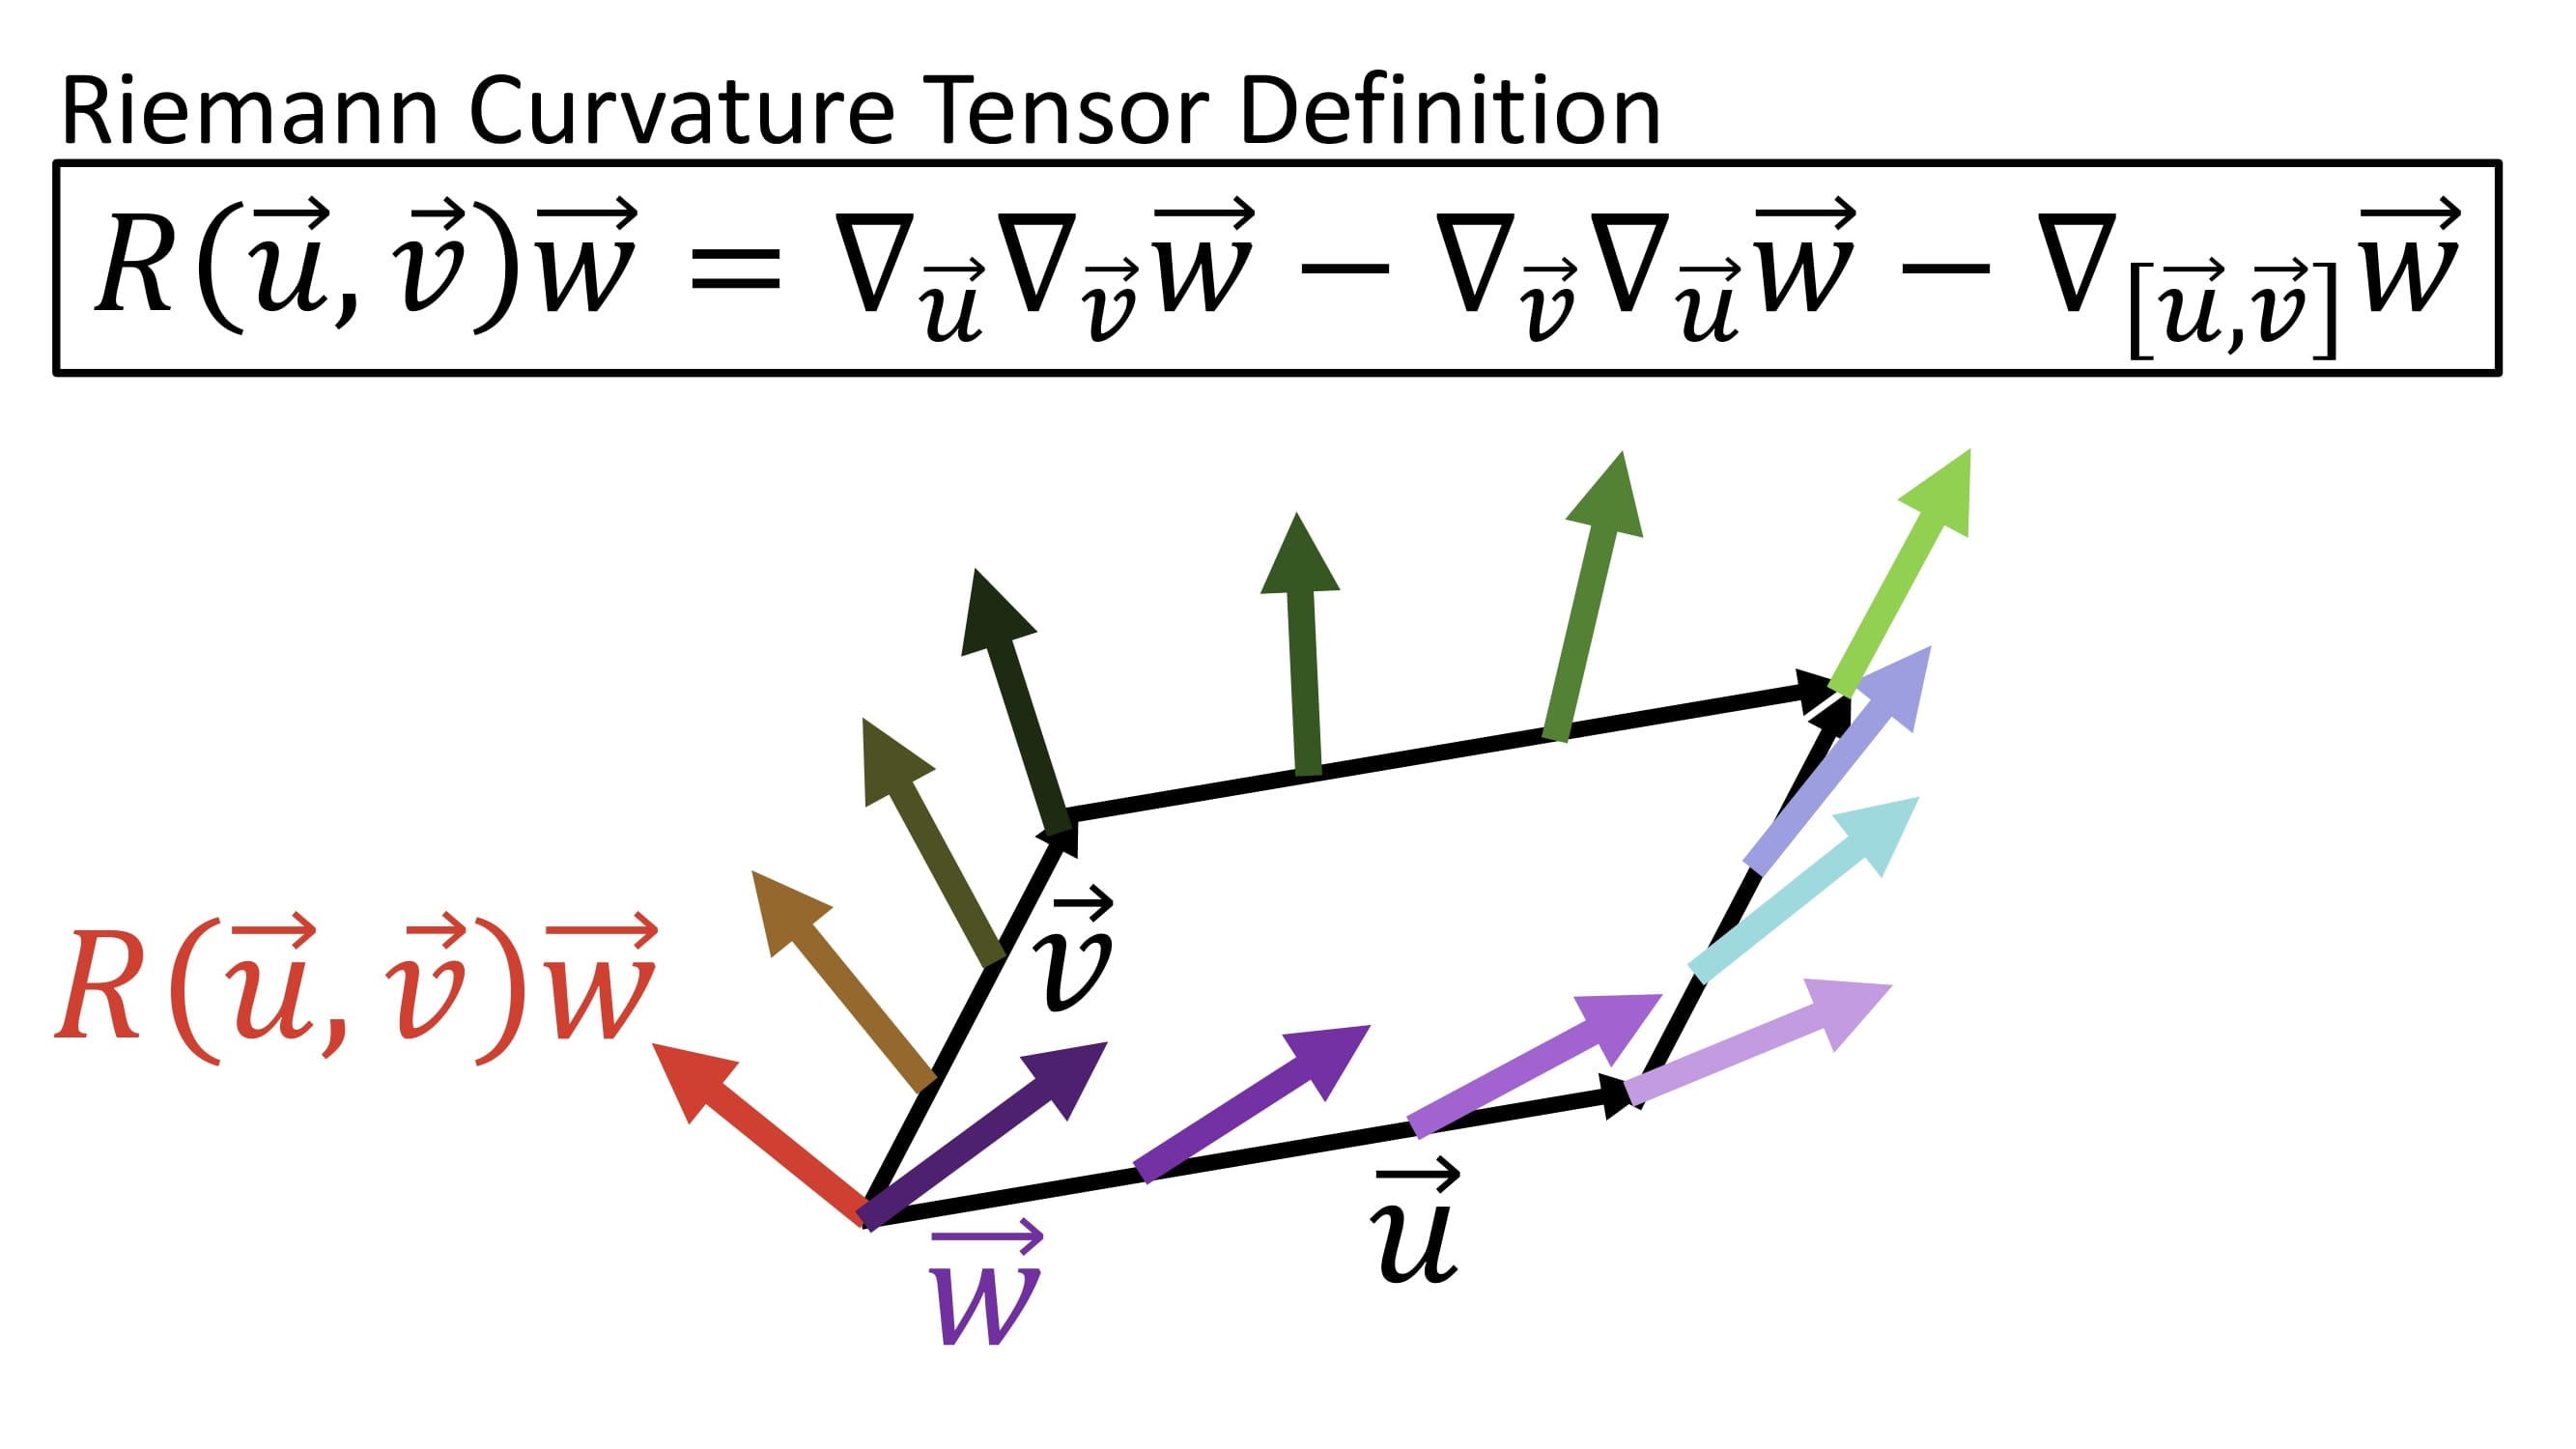
\includegraphics[width=0.7\textwidth]{Figs/c1.jpg}
    \caption{\small Holonomy definition visualization (if Lie bracket is 0)}
    \label{fig:gadfadf}
\end{figure}
\item \tb{Geodesic Deviation:} See \cref{fig:asgrre}. If we assume torch free, we have the geodesic deviation $$\nabla_{\vec{v}}\nabla_{\vec{v}} \vec{s}=  -R(\vec{s}, \vec{v})\vec{v}.$$ 
    \begin{figure}[H]
     \centering
     \begin{subfigure}[b]{0.45\textwidth}
         \centering
         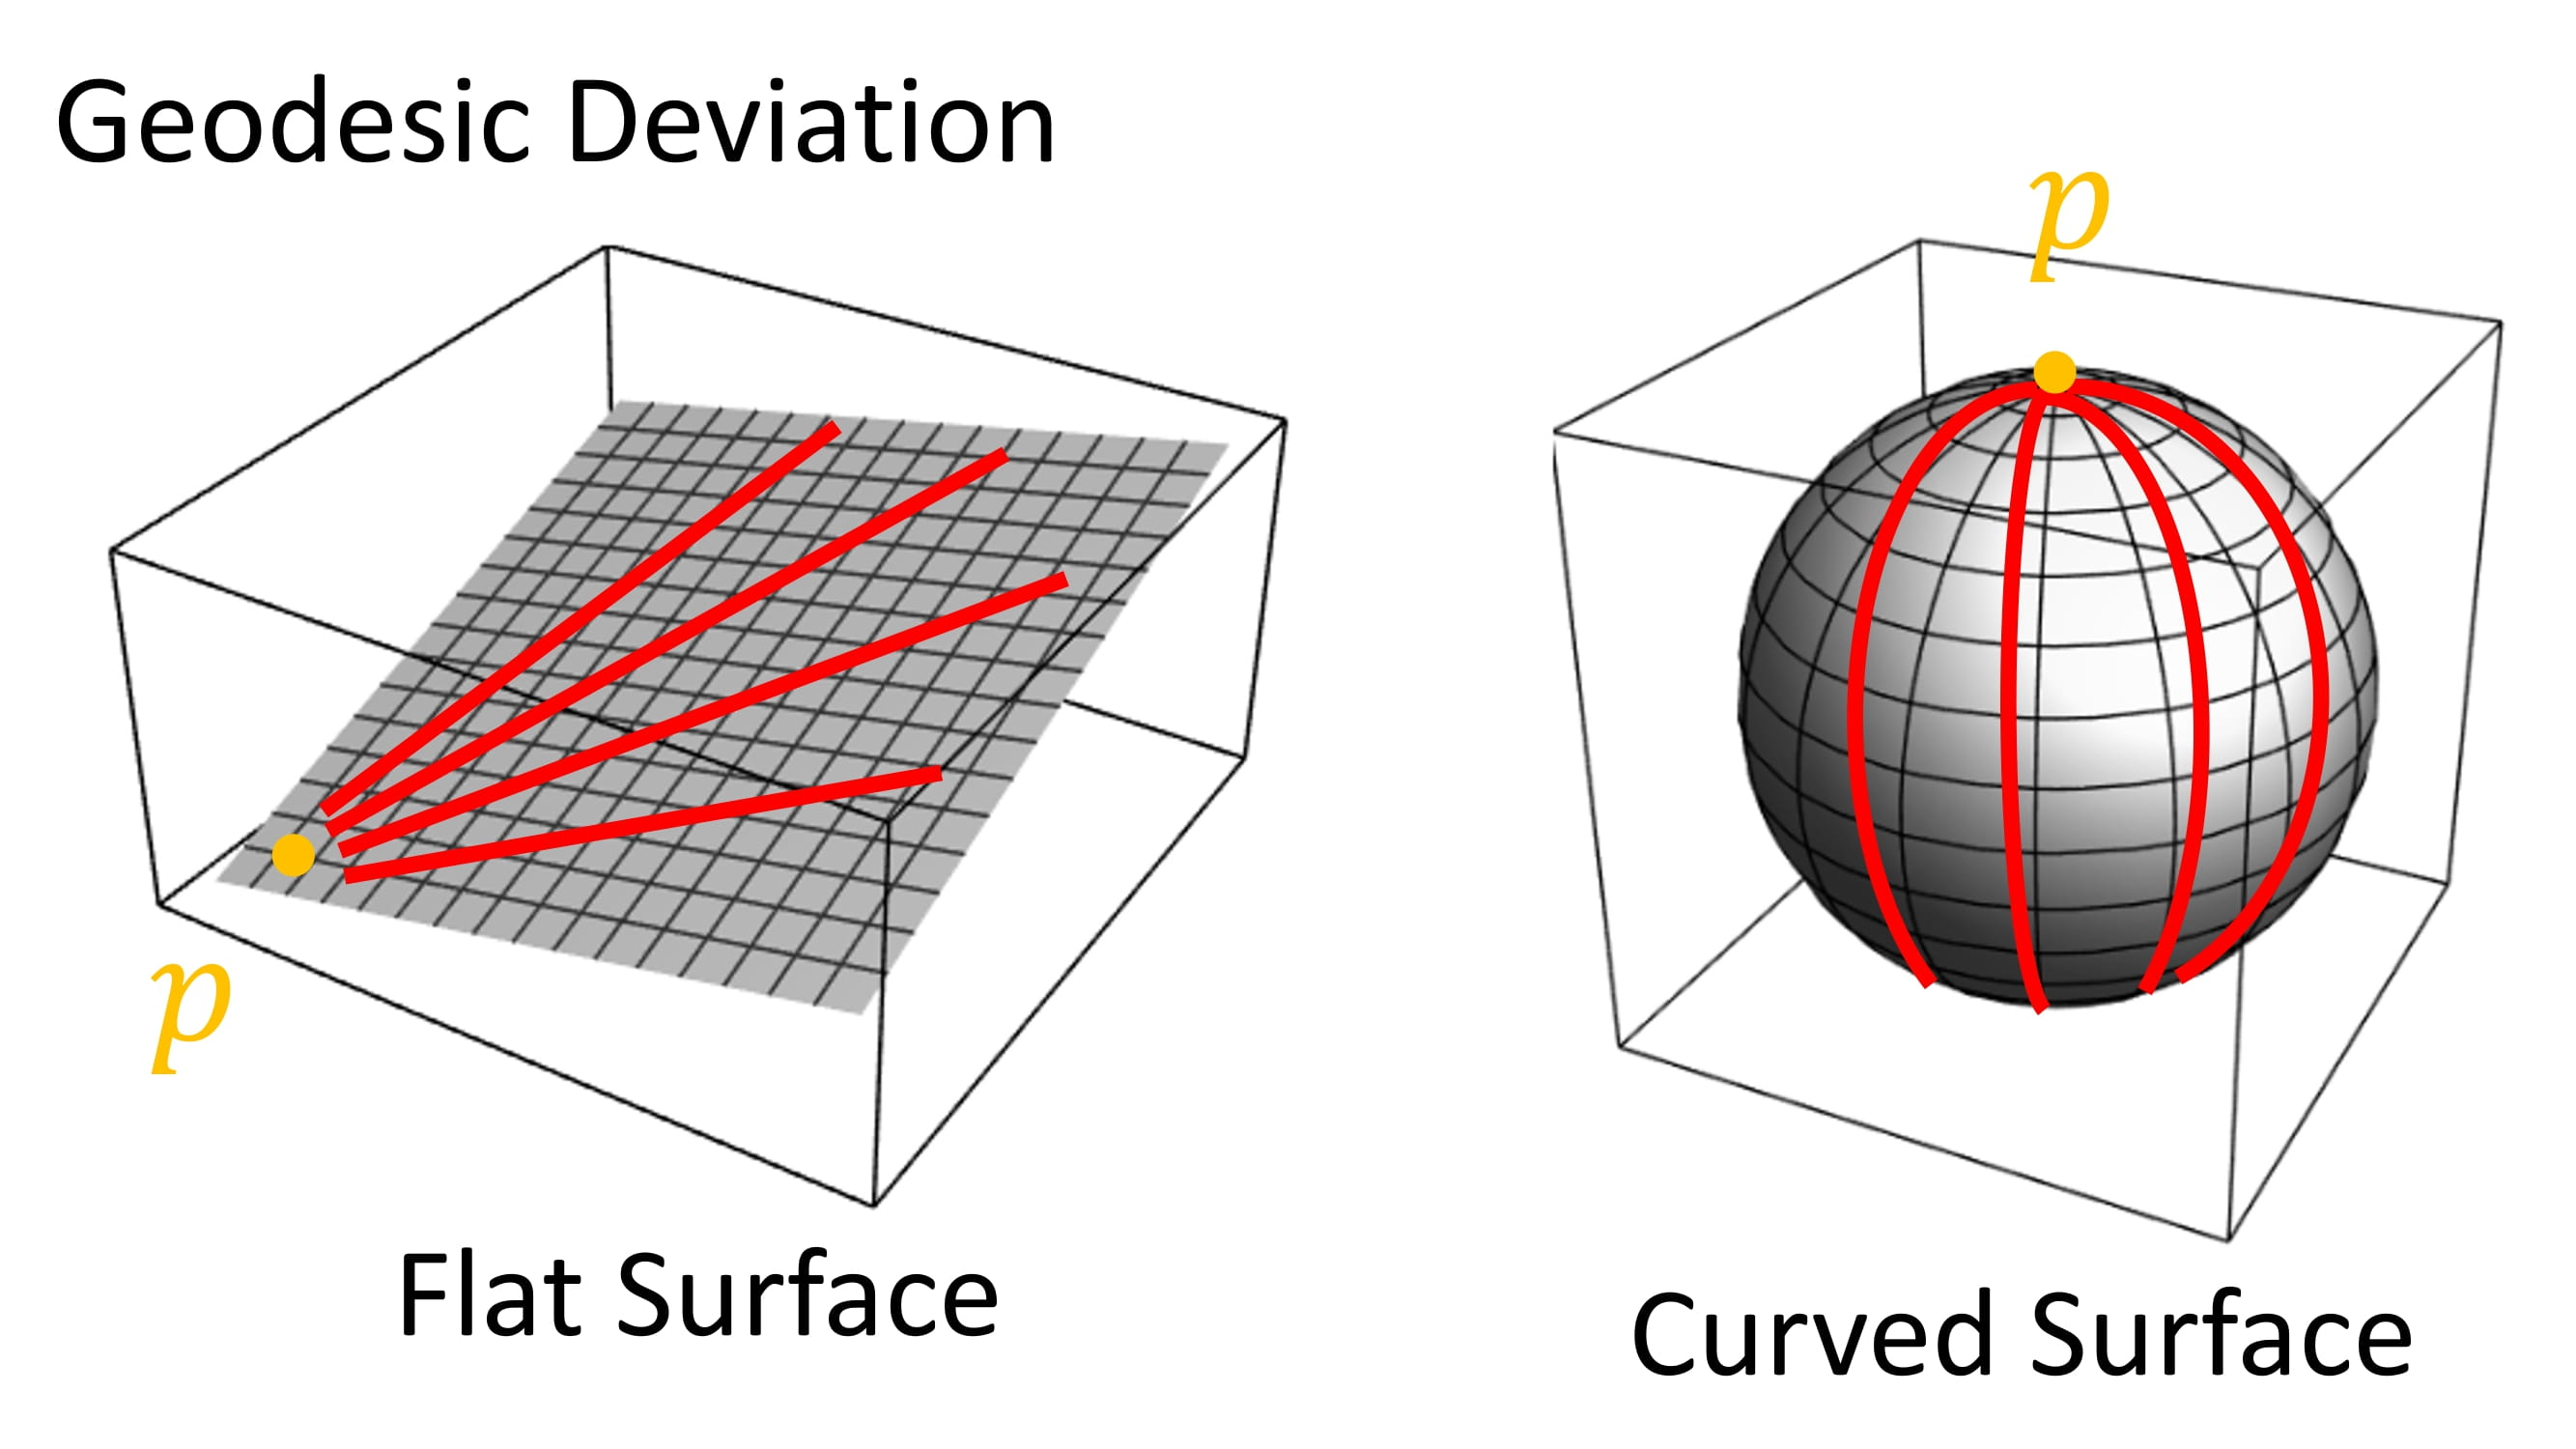
\includegraphics[width=\textwidth]{Figs/c2.jpg}
     \end{subfigure}
     \hfill
     \begin{subfigure}[b]{0.45\textwidth}
         \centering
         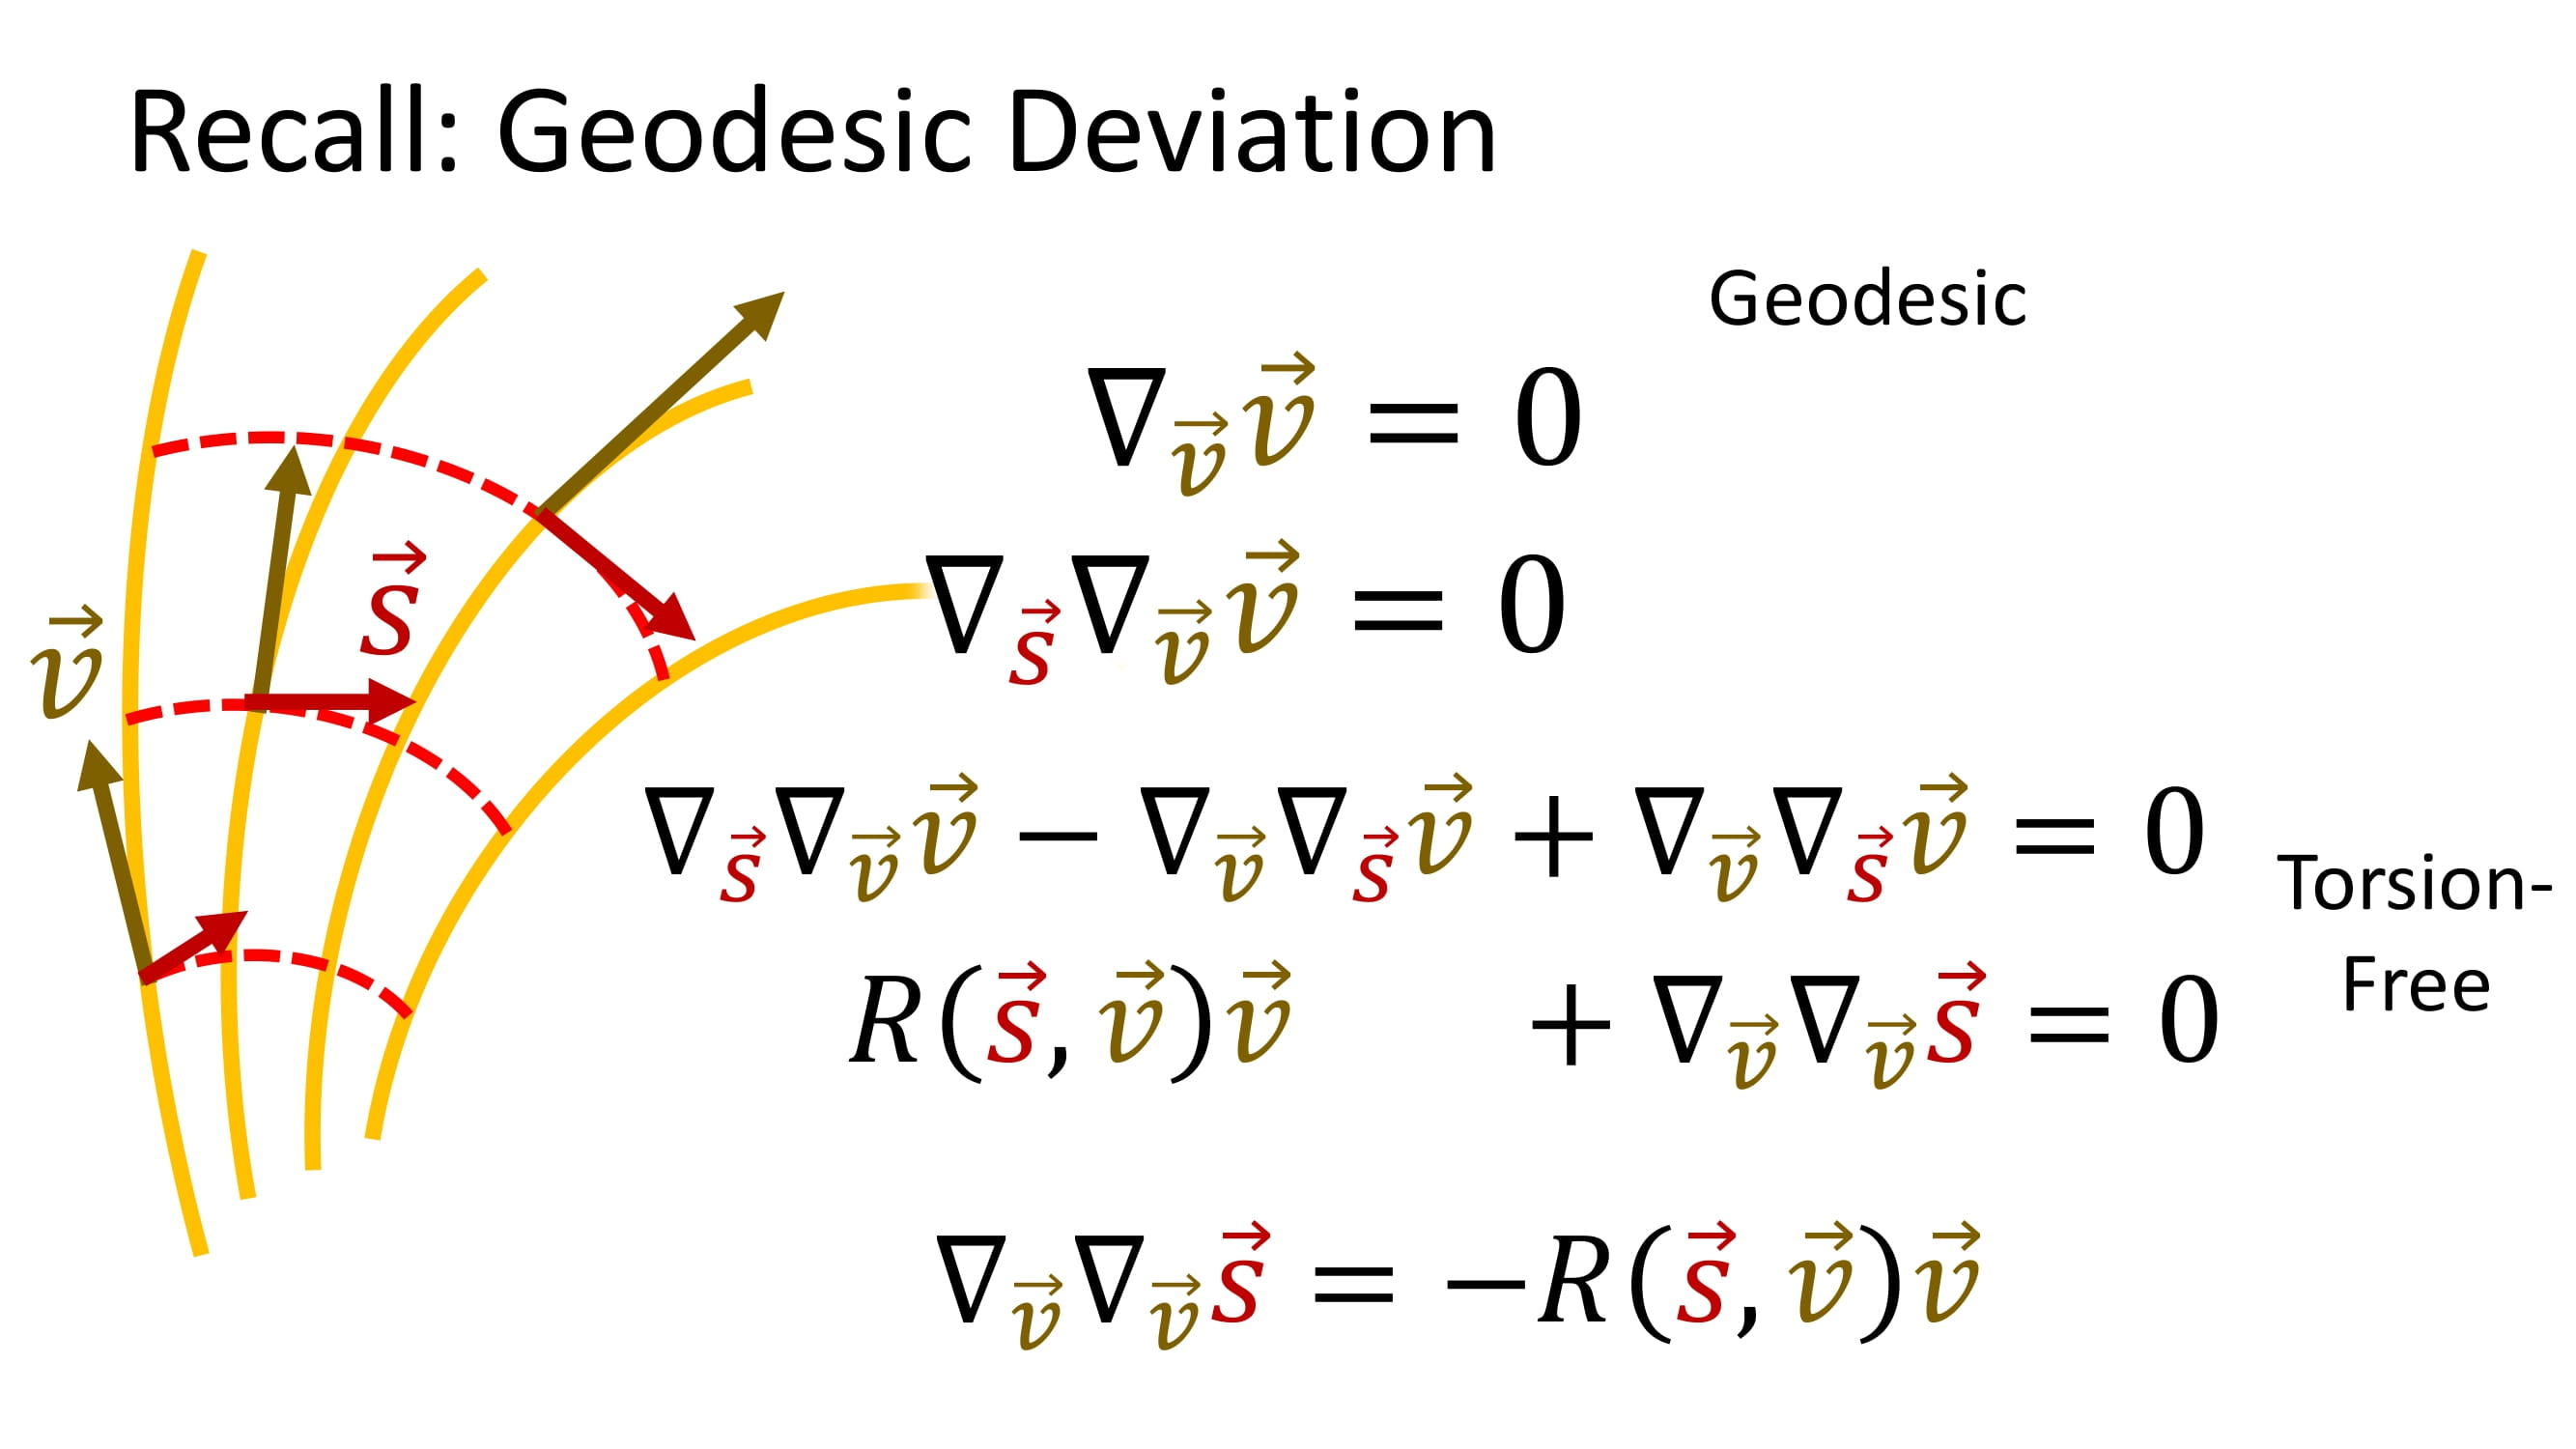
\includegraphics[width=\textwidth]{Figs/c3.jpg}
     \end{subfigure}
     \caption{\small Geodesic deviation} \label{fig:asgrre}
\end{figure}
     \begin{figure}[H]
    \centering
    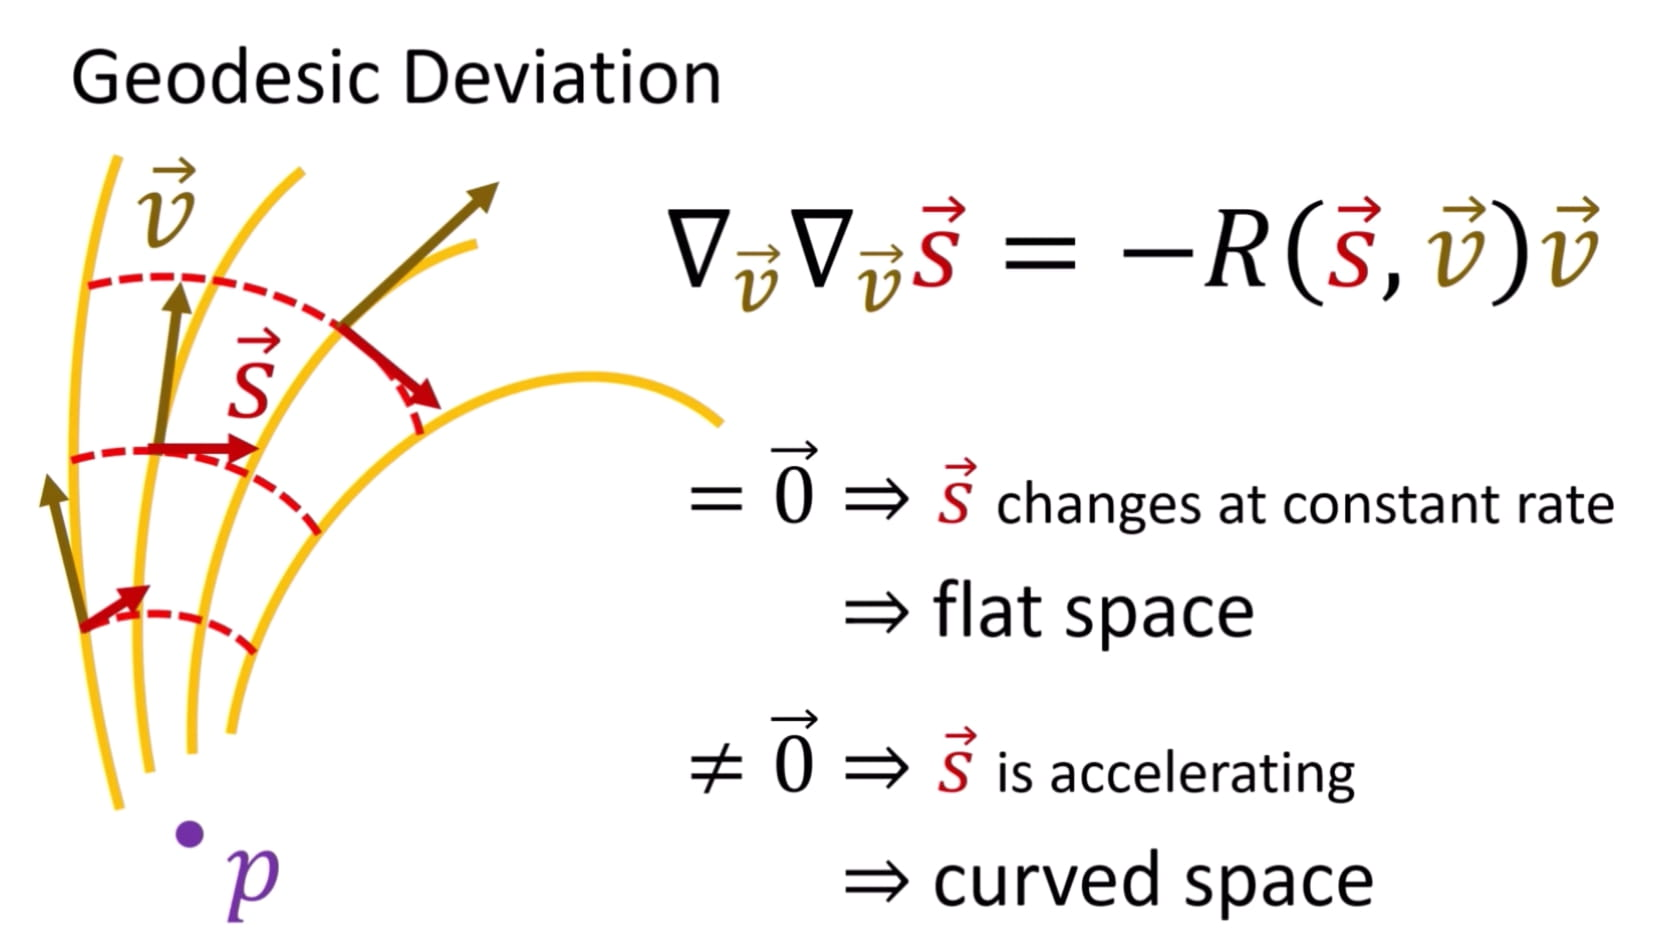
\includegraphics[width=0.7\textwidth]{Figs/c4.jpg}
    \caption{\small Flat or curved using geodesic deviation.}
    \label{fig:trwred}
\end{figure}
    \end{enumerate}
    \item \tb{Sectional curvature:} The sectional curvature depends on a two-dimensional linear subspace $K(\sigma_p)$ of the tangent space at a point $p$ of the manifold. It can be defined geometrically as the \tb{Gaussian curvature} of the surface which has the plane $K(\sigma_p)$ as a tangent plane at $p$, obtained from \tb{geodesics} which start at $p$ in the directions of $K(\sigma_p)$ (in other words, the image of $K(\sigma_p)$ under the exponential map at $p$). The sectional curvature is a real-valued function.  See \cref{fig:dagrteqr} and \cref{fig:eqrqerq} for more details.
        \begin{figure}[H]
     \centering
     \begin{subfigure}[b]{0.45\textwidth}
         \centering
         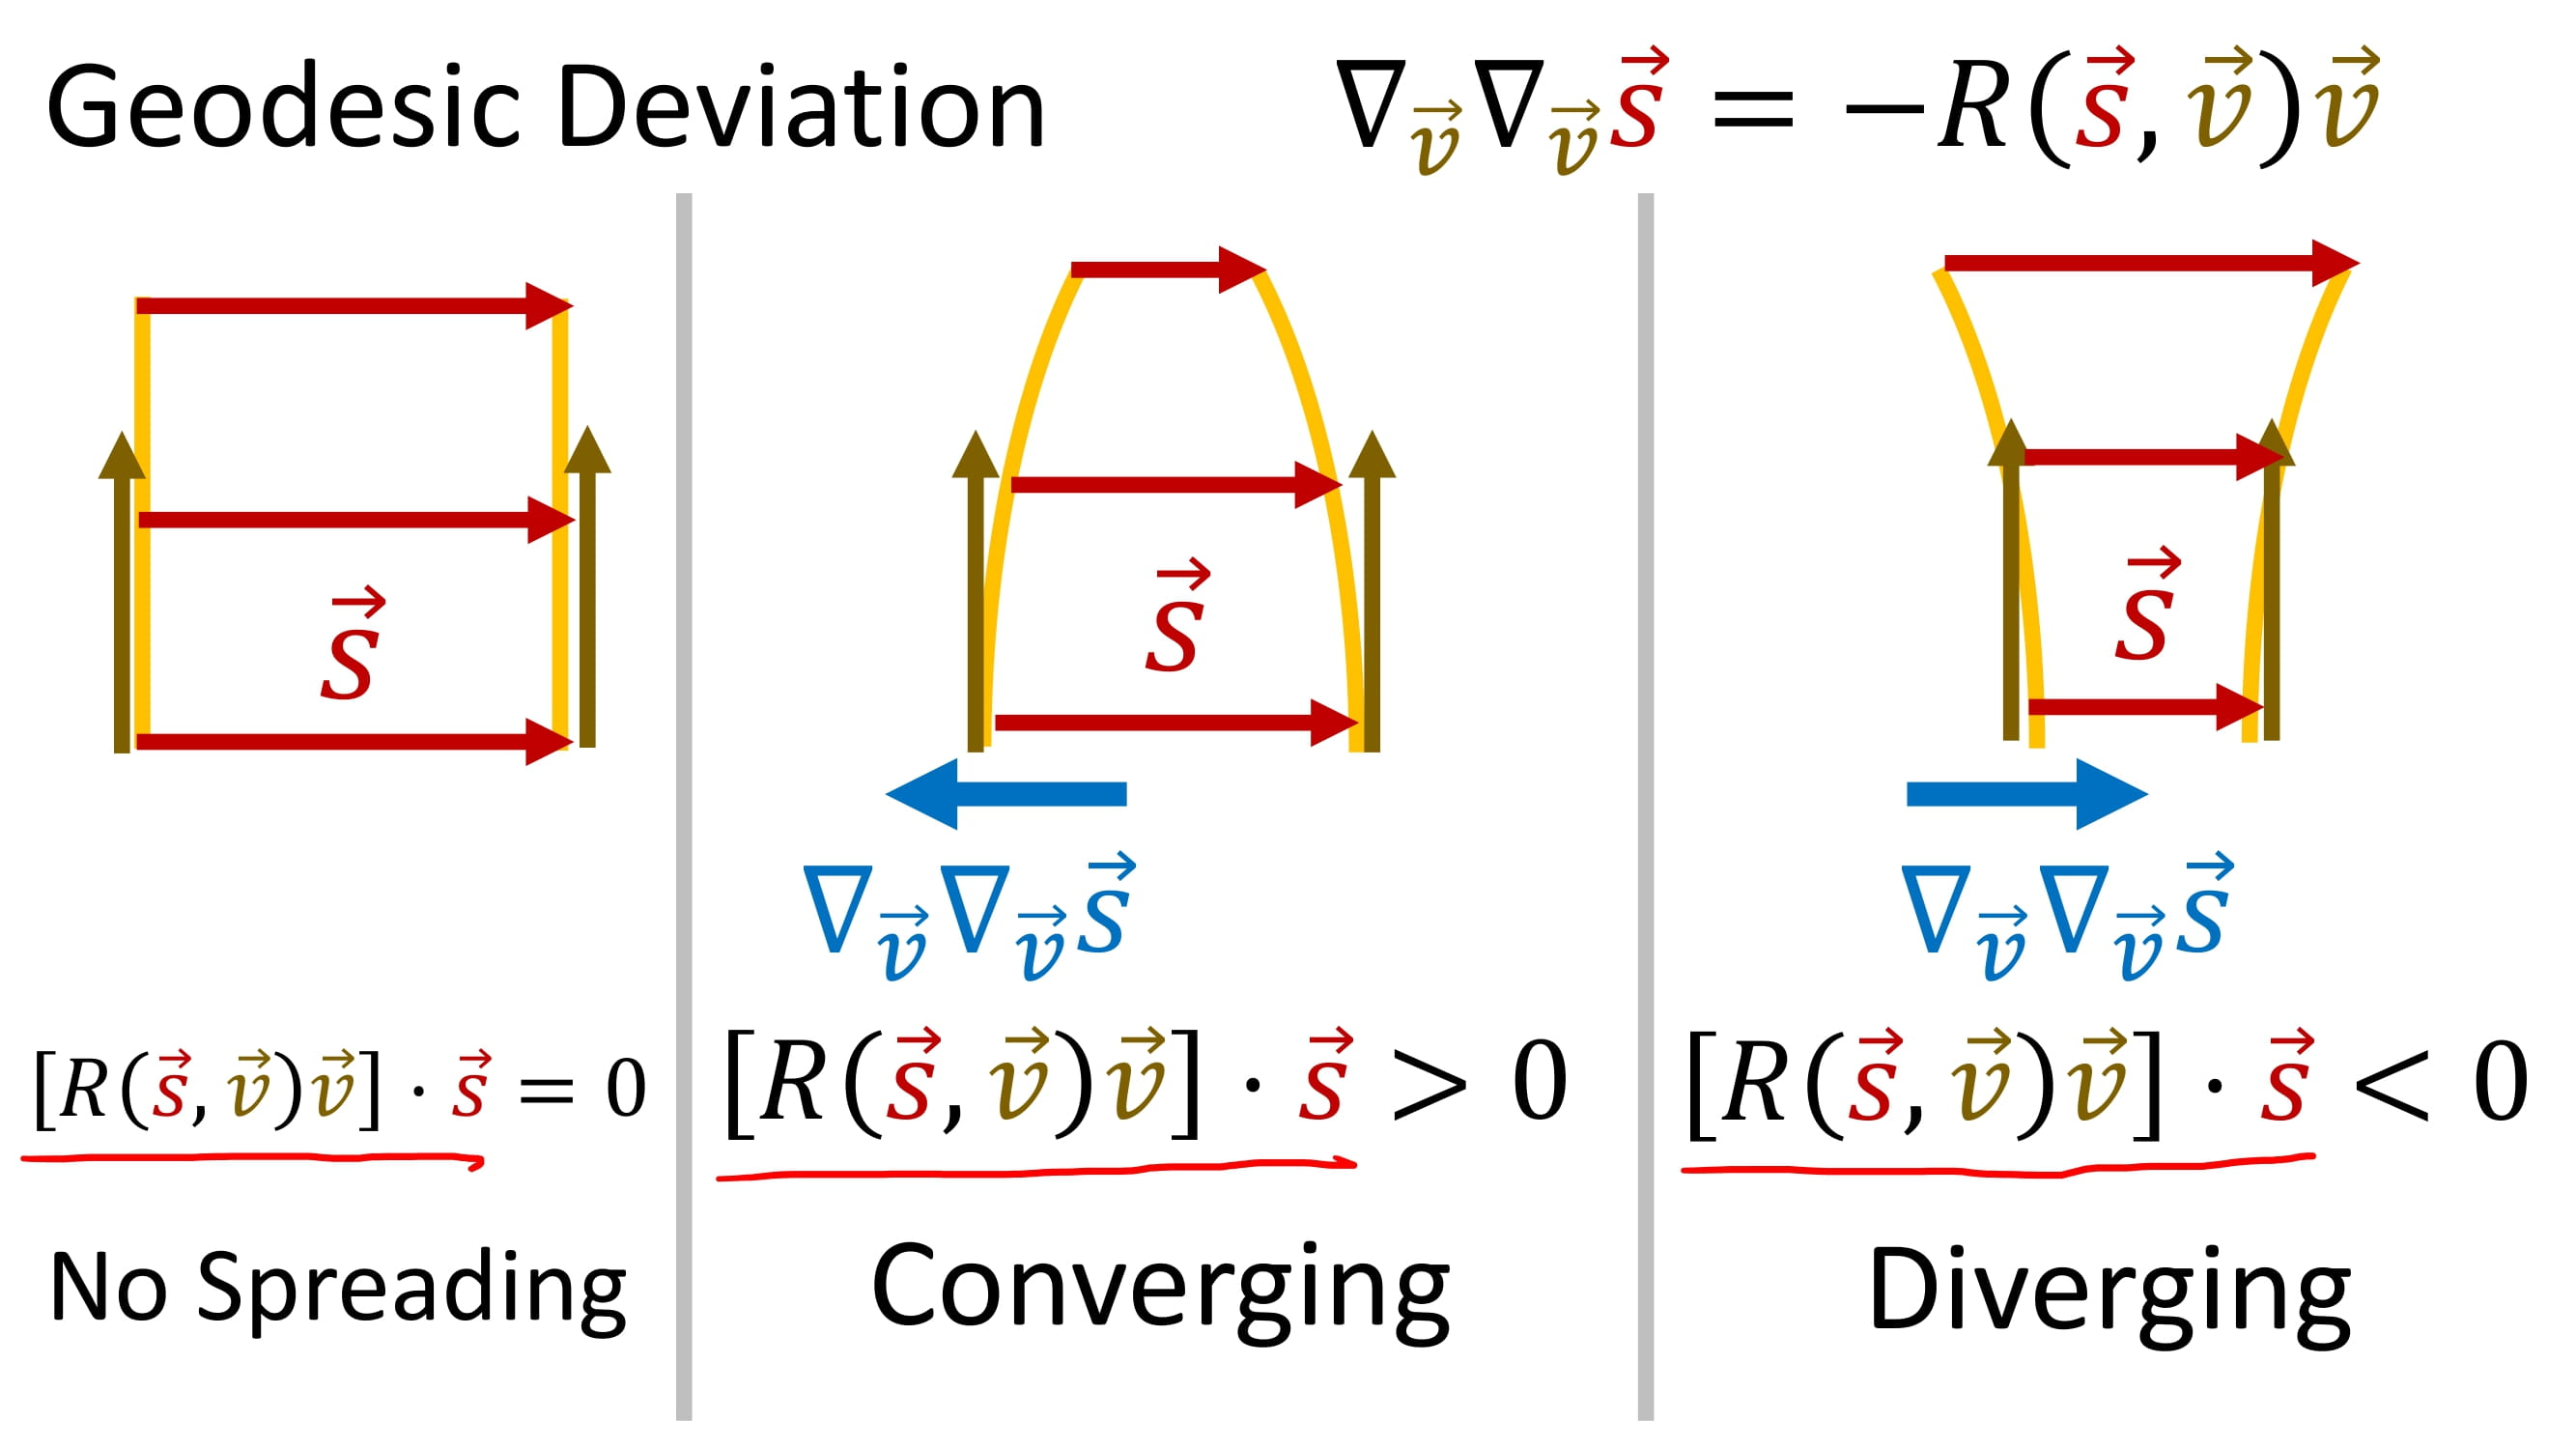
\includegraphics[width=\textwidth]{Figs/s1.jpg}
     \end{subfigure}
     \hfill
     \begin{subfigure}[b]{0.45\textwidth}
         \centering
         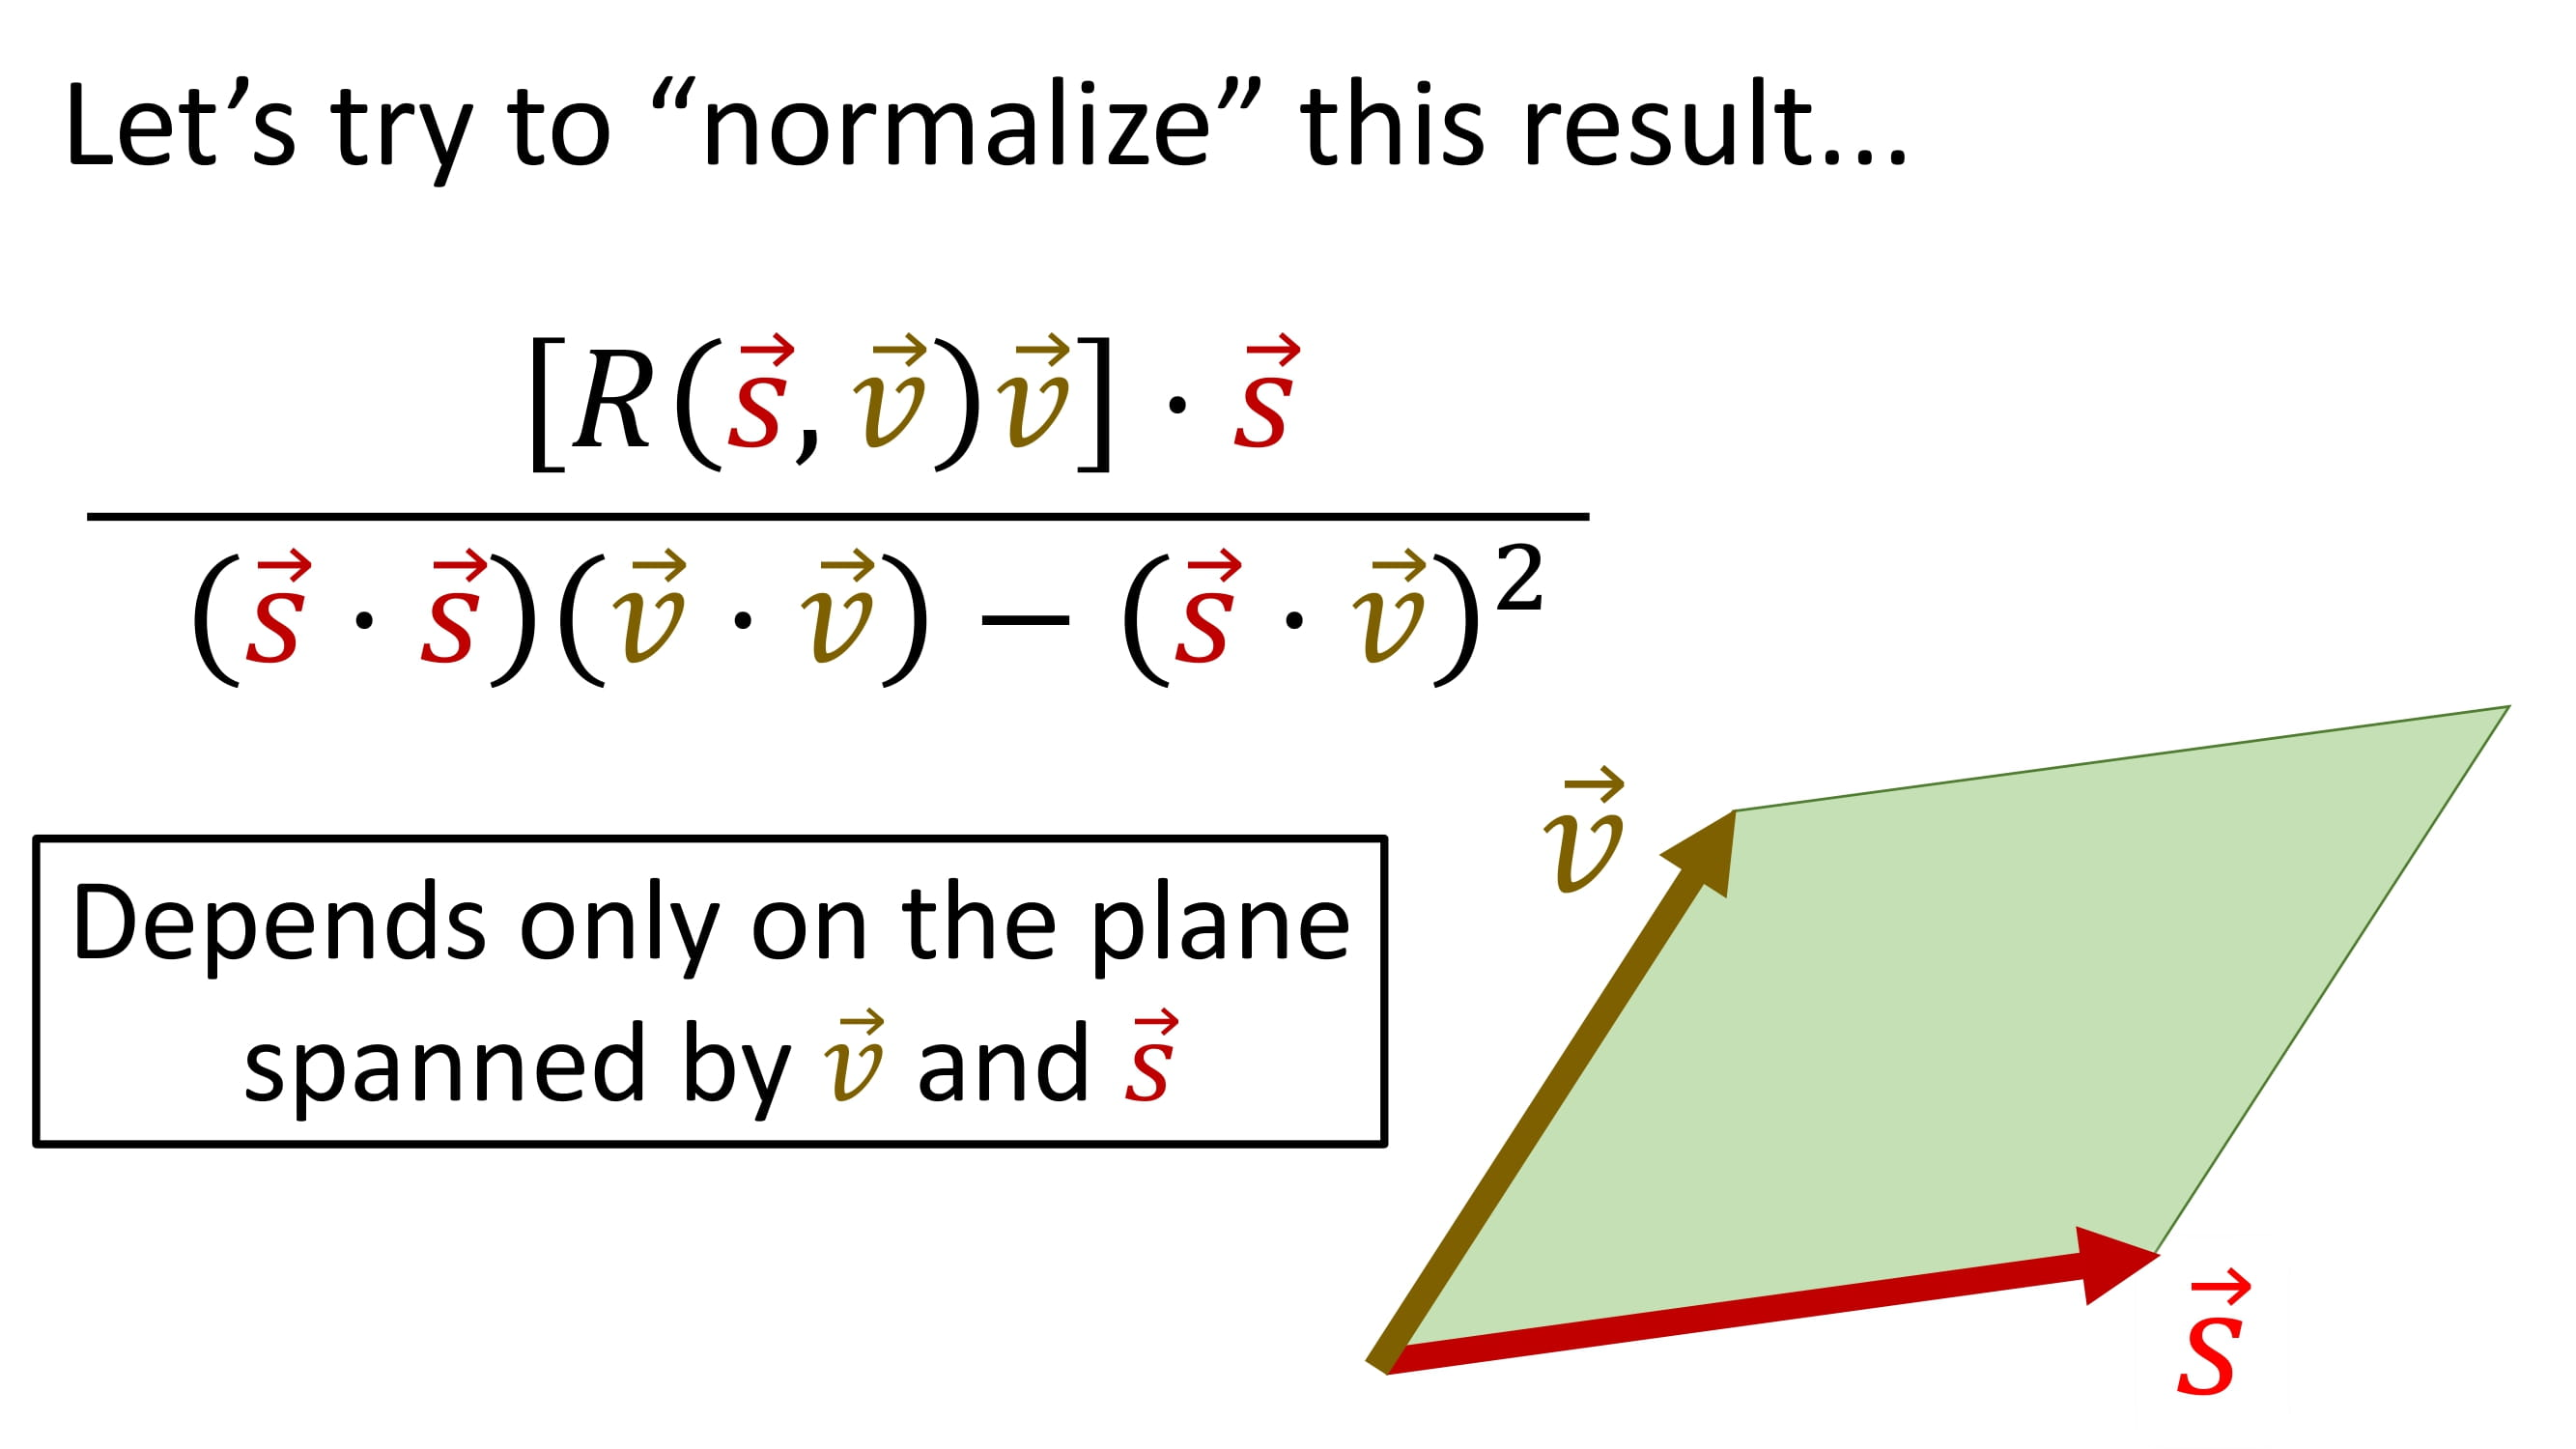
\includegraphics[width=\textwidth]{Figs/s2.jpg}
     \end{subfigure}
     \caption{\small Sectional curvature from geodesic deviation normalized by the area of parallelogram.} \label{fig:dagrteqr}
\end{figure}
    
         \begin{figure}[H]
    \centering
    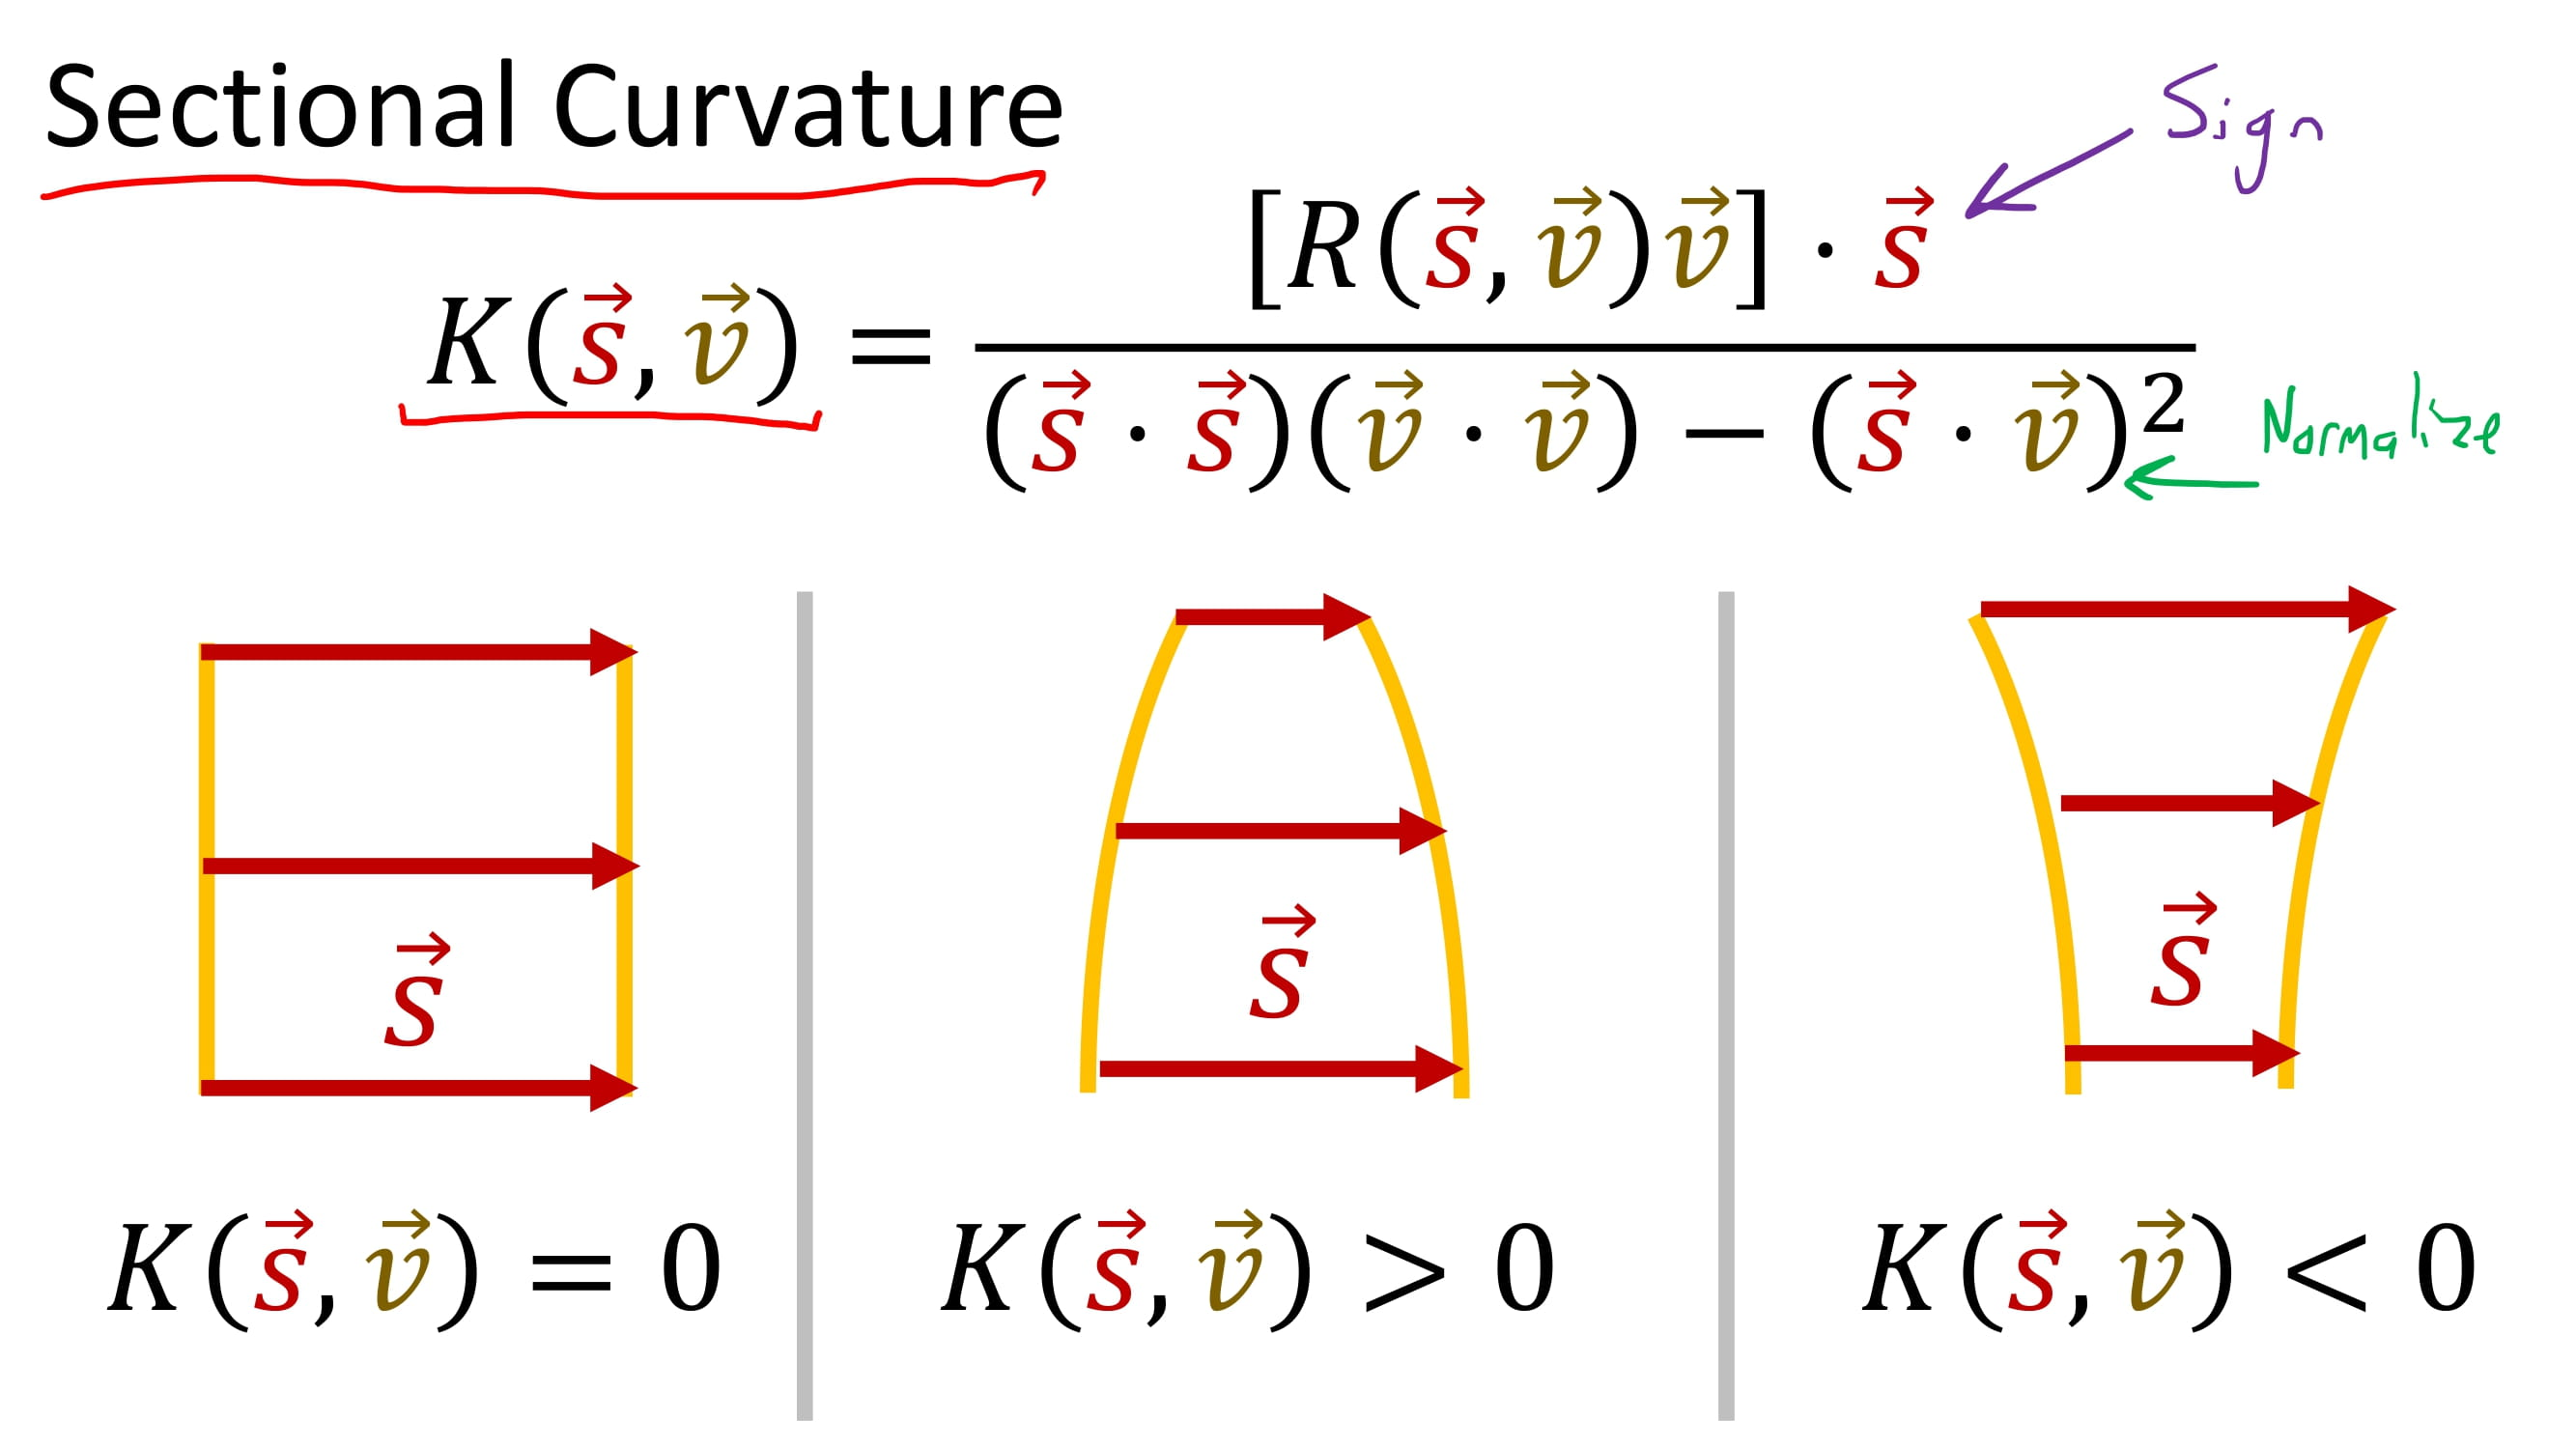
\includegraphics[width=0.7\textwidth]{Figs/s3.jpg}
    \caption{\small  Sectional curvature visualization.}
    \label{fig:eqrqerq}
\end{figure}
    \item \tb{Ricci curvature:}  It can be considered, broadly, as a measure of the degree to which the geometry of a given metric tensor differs locally from that of ordinary Euclidean space or pseudo-Euclidean space. The Ricci tensor can be characterized by \tb{measurement of how a shape is deformed as one moves along geodesics in the space.} % Like the metric tensor, the Ricci tensor assigns to each tangent space of the manifold \tb{a symmetric bilinear form}. Broadly, one could analogize the role of the Ricci curvature in Riemannian geometry to that of the Laplacian in the analysis of functions; in this analogy, the Riemann curvature tensor, of which the Ricci curvature is a natural by-product, would correspond to the full matrix of second derivatives of a function.
    Ricci curvature can tell us about \tb{size} changes, but can’t tell us about \tb{shape} changes.
    We have two explanations:
    \begin{enumerate}[label=(\textbf{\alph*})]
        \item \tb{sum (or average) of sectional curvature using orthonormal basis:} 
        
        Ricci curvature is like an average of all possible sectional curvatures containing the vector $\vec{v}$. In other words, let's take an orthonormal basis $\left\{\overrightarrow{e_{1}}, \overrightarrow{e_{2}}, \ldots, \overrightarrow{e_{n}}\right\}$ and a direction vector $\vec{v}=\overrightarrow{e_{n}}$, we then have
$$
\Ric(\vec{v}, \vec{v})=\sum_{i=1}^{D} K\left(\overrightarrow{e_{i}}, \vec{v}\right)=\sum_{i} \frac{\left[R\left(\overrightarrow{e_{i}}, \vec{v}\right) \vec{v}\right] \cdot \overrightarrow{e_{i}}}{\left(\overrightarrow{e_{i}} \cdot \overrightarrow{e_{i}}\right)(\vec{v} \cdot \vec{v})-\left(\overrightarrow{e_{i}} \cdot \vec{v}\right)^{2}}
$$

    \begin{figure}[H]
     \centering
     \makebox[\textwidth][c]{
     \begin{subfigure}[b]{0.245\textwidth}
         \centering
         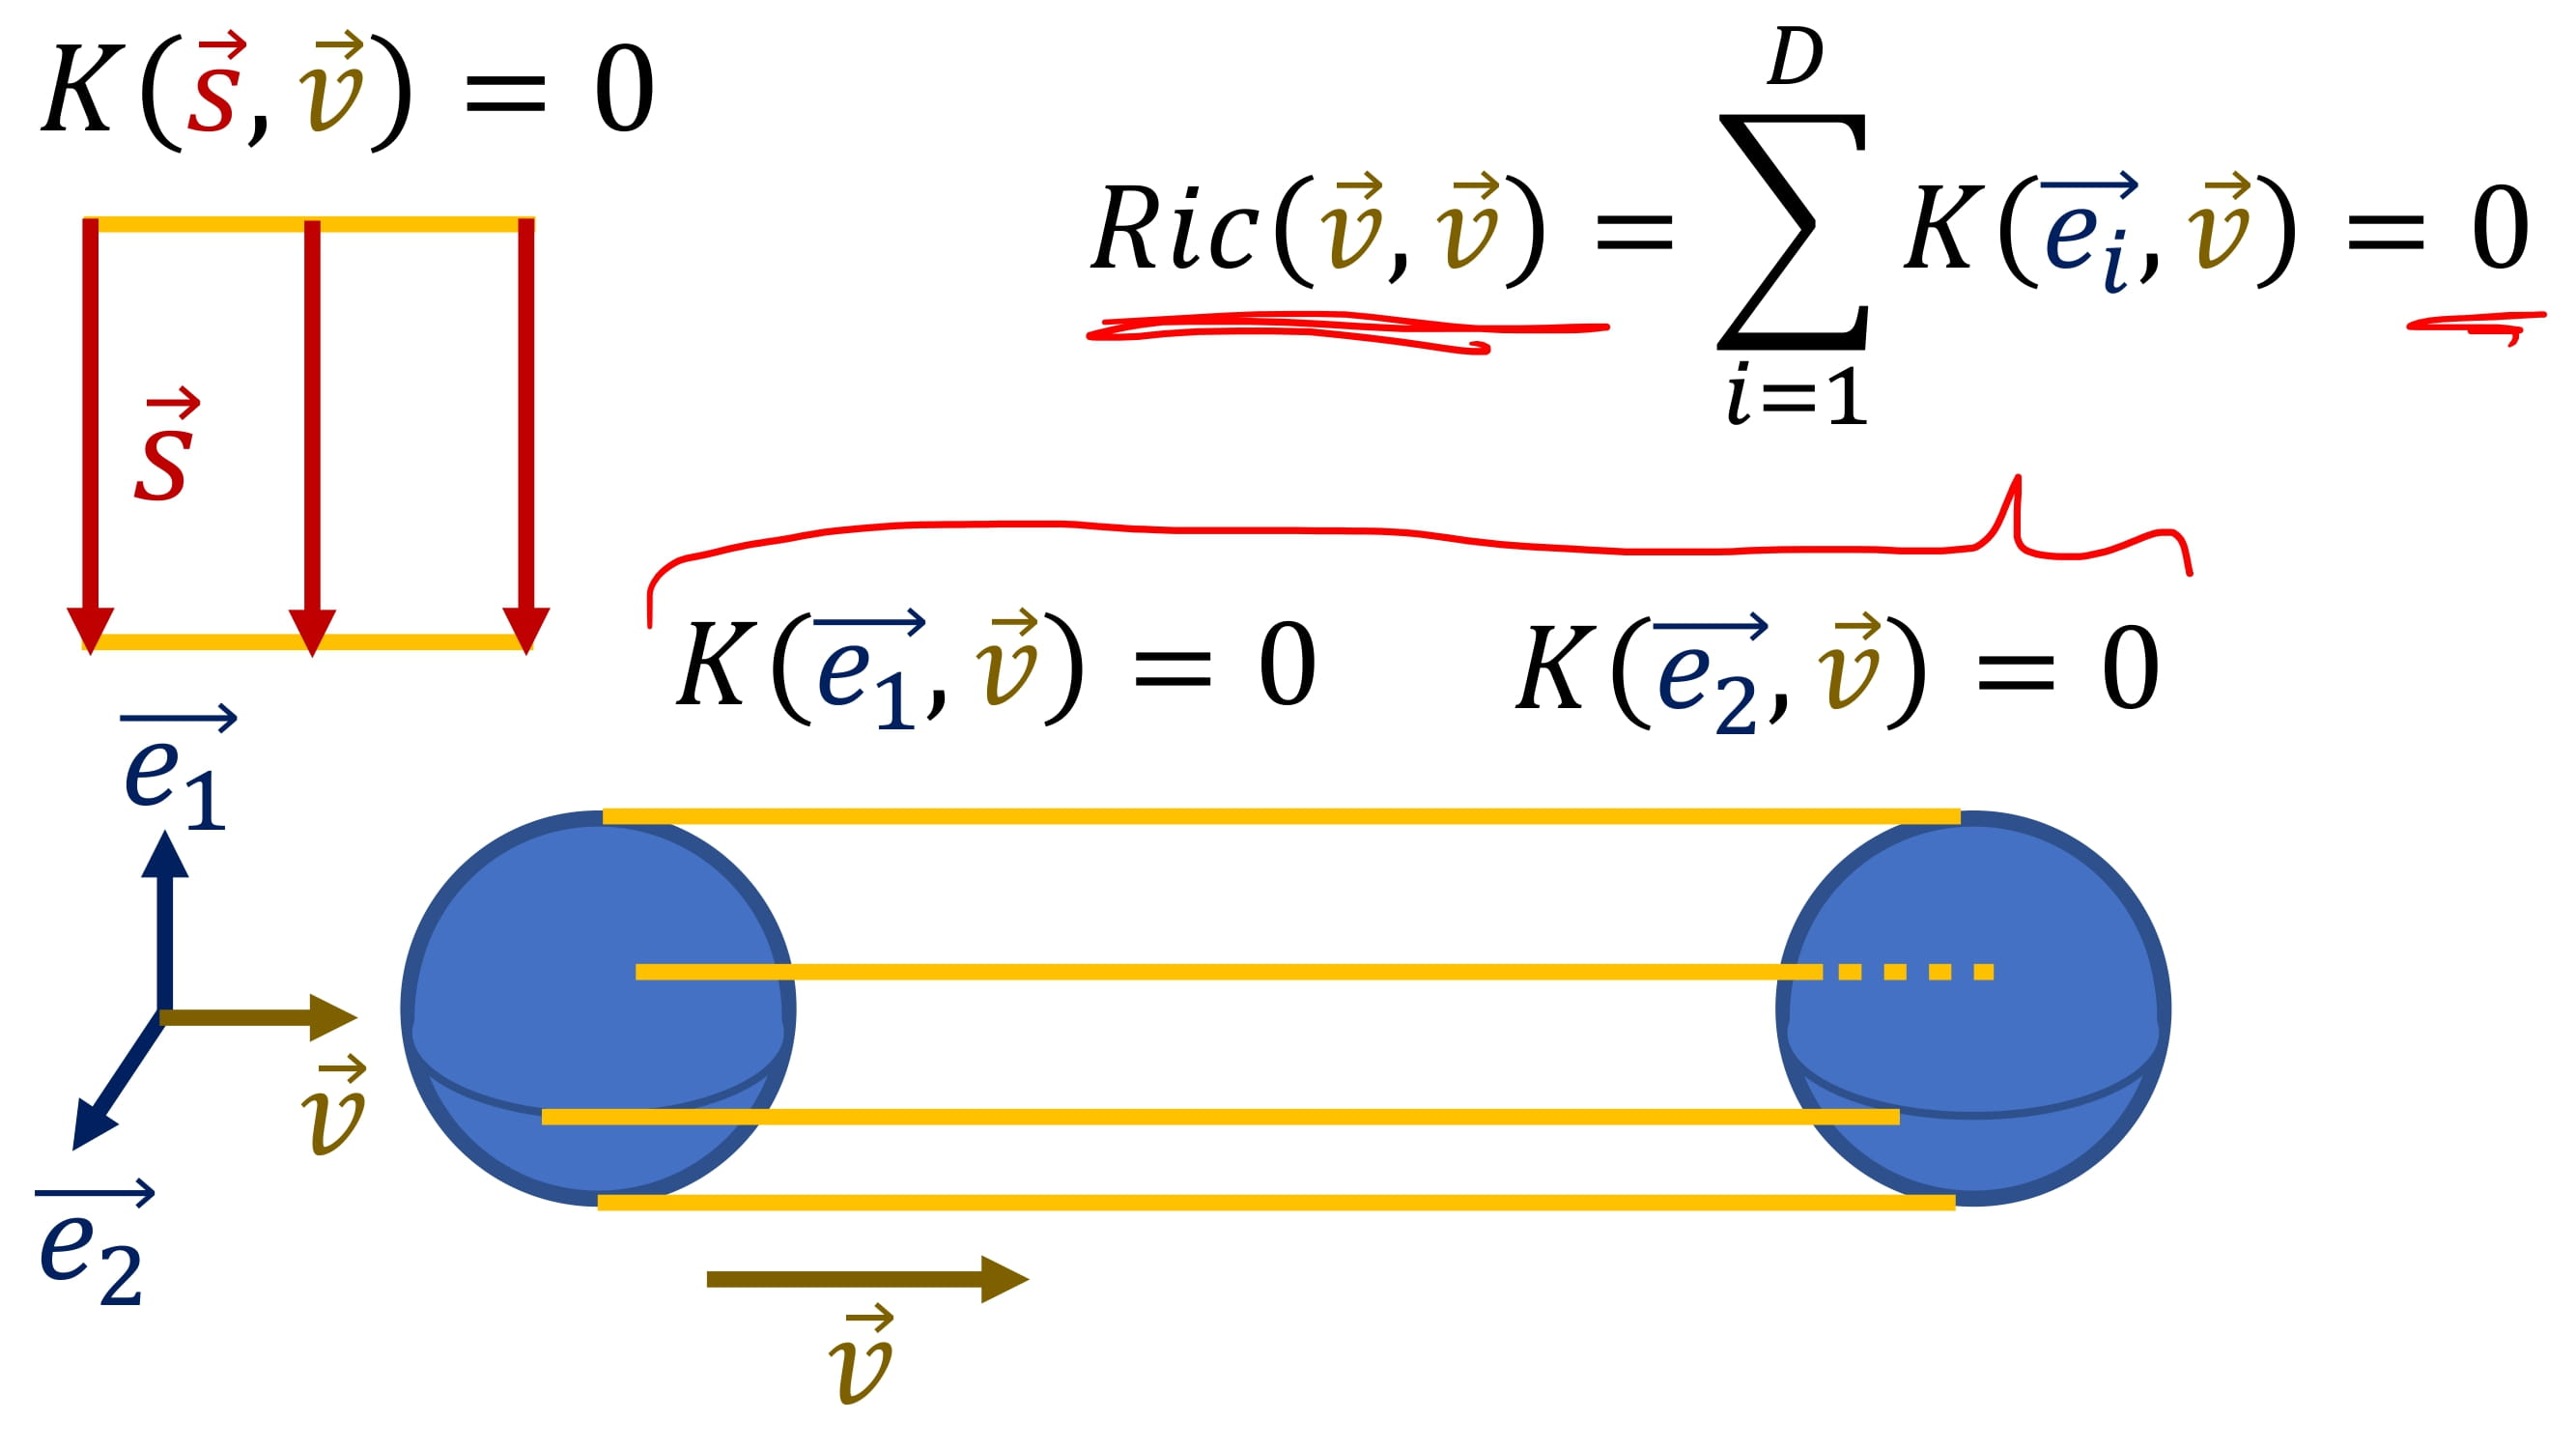
\includegraphics[width=\textwidth]{Figs/r1.jpg}
     \end{subfigure}
     \hfill
     \begin{subfigure}[b]{0.245\textwidth}
         \centering
         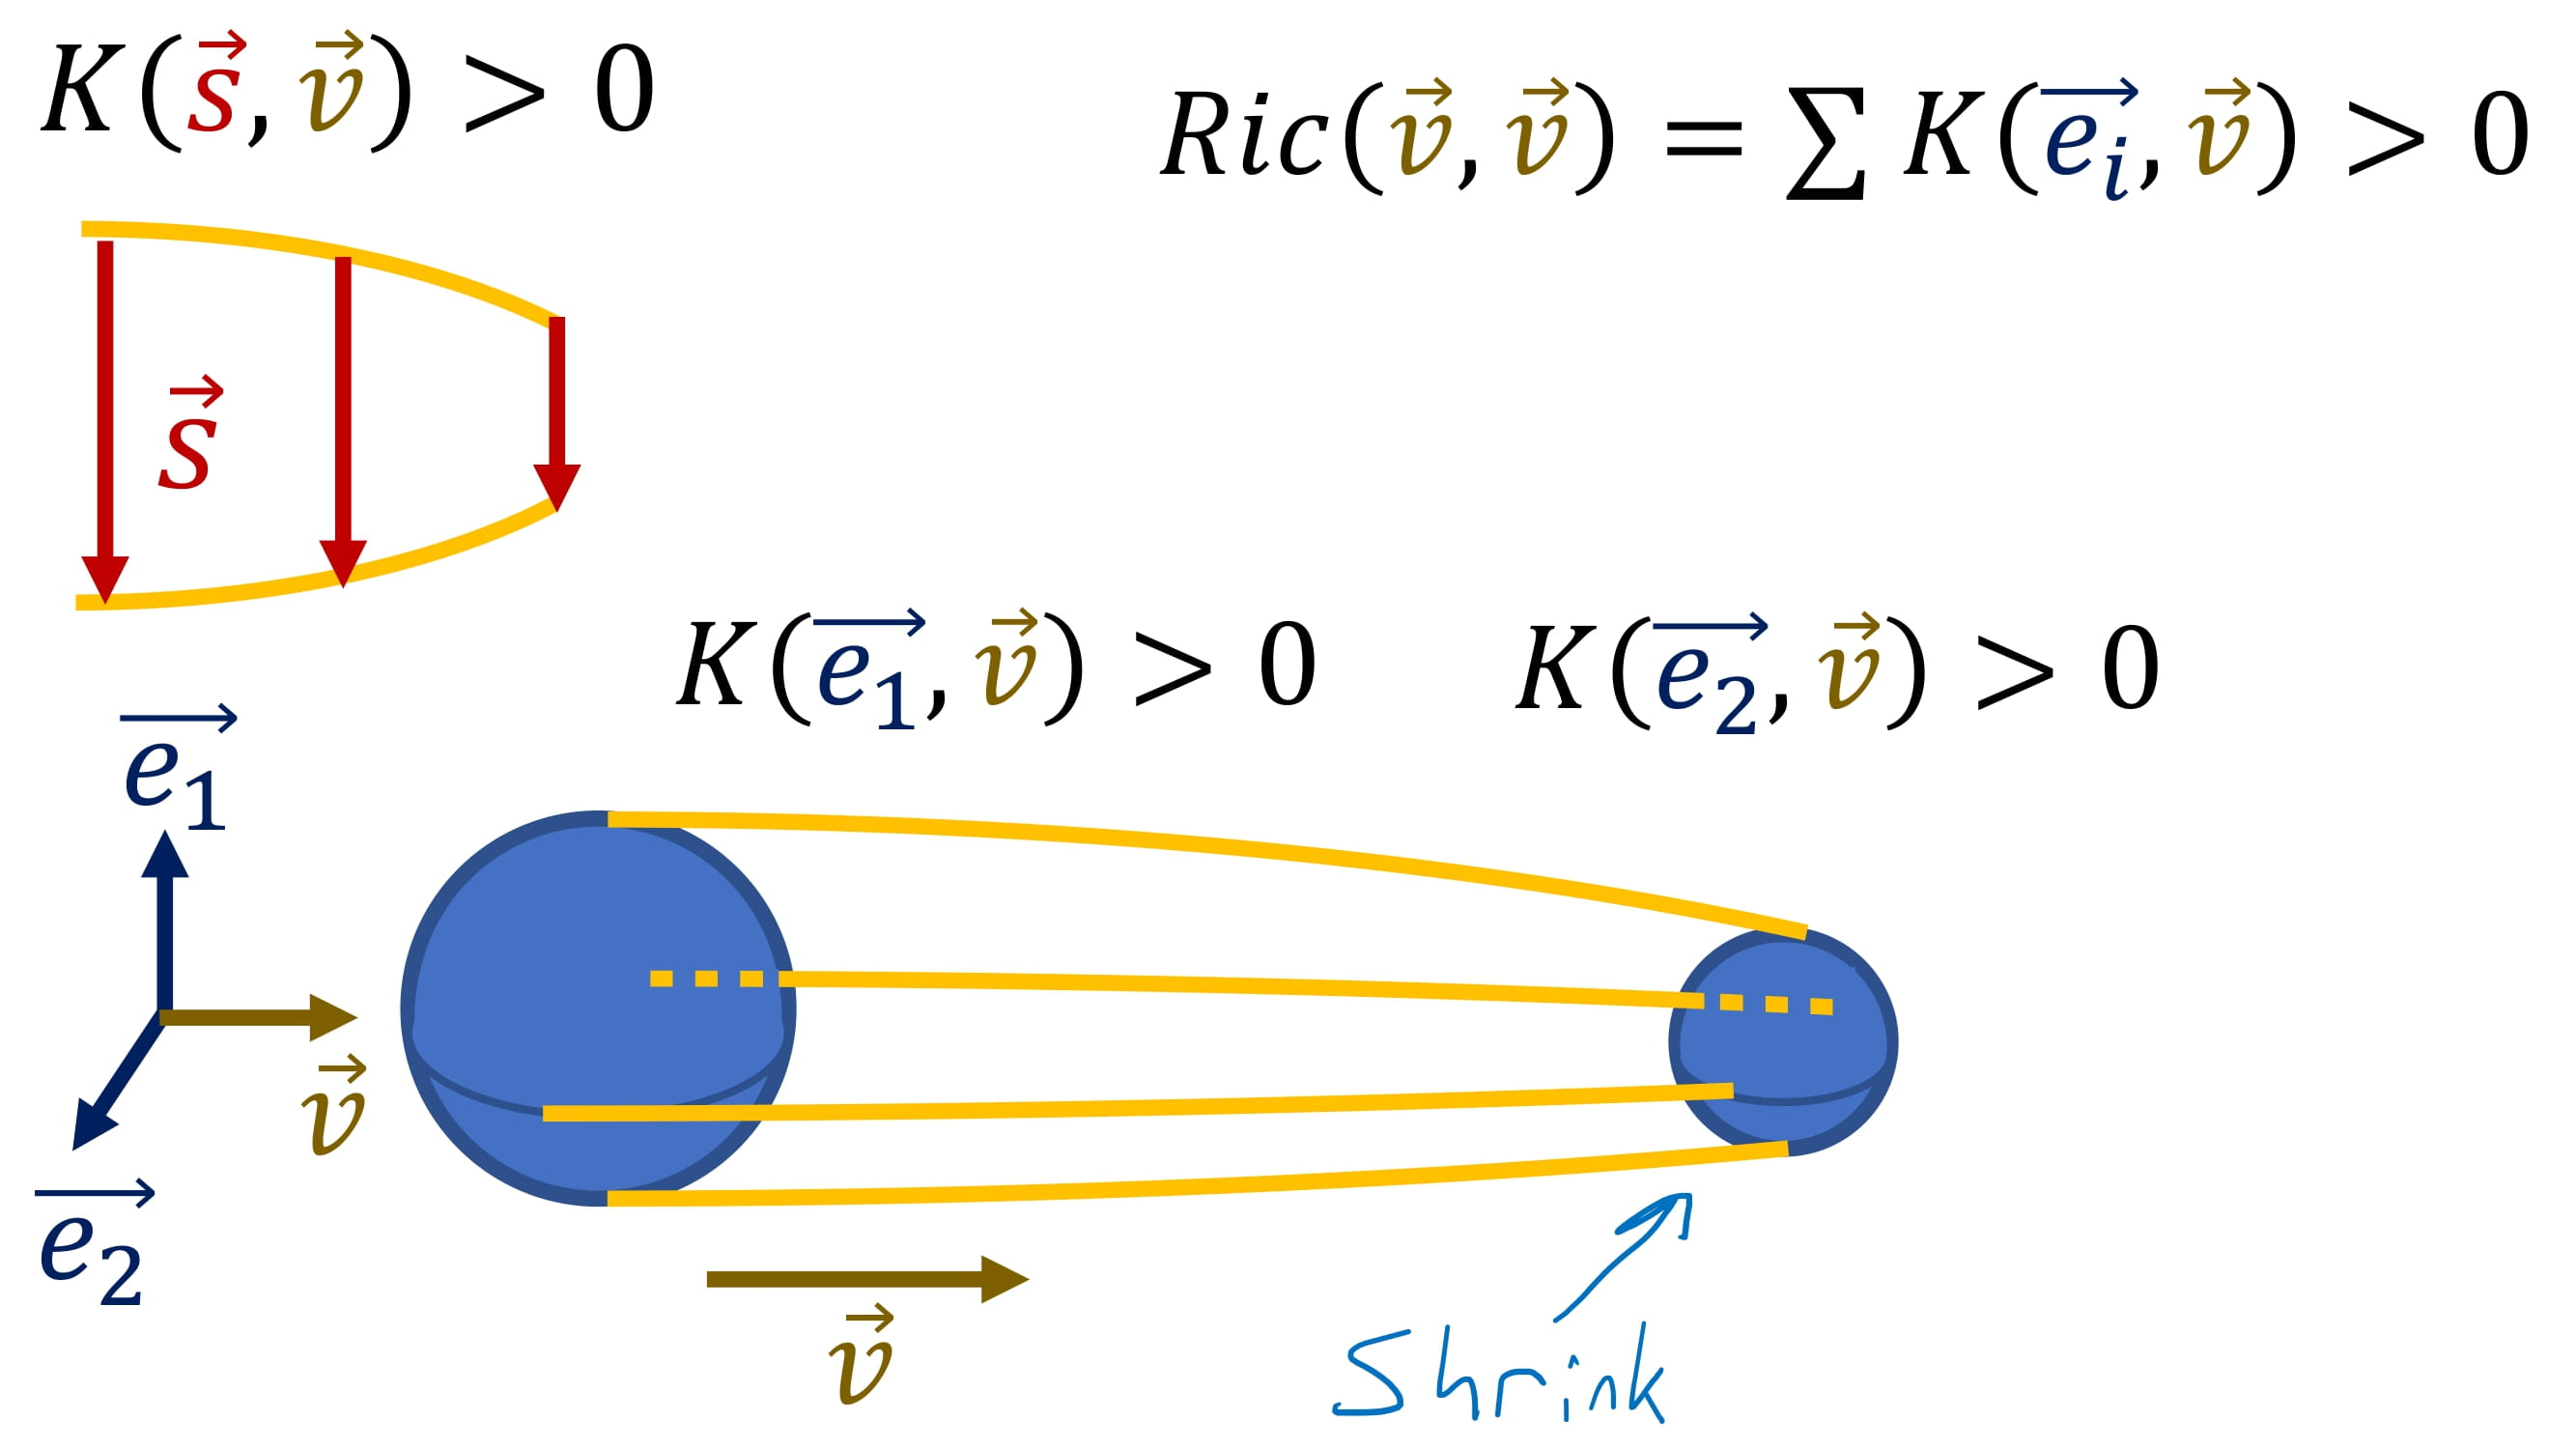
\includegraphics[width=\textwidth]{Figs/r2.jpg}
     \end{subfigure}
      \begin{subfigure}[b]{0.245\textwidth}
         \centering
         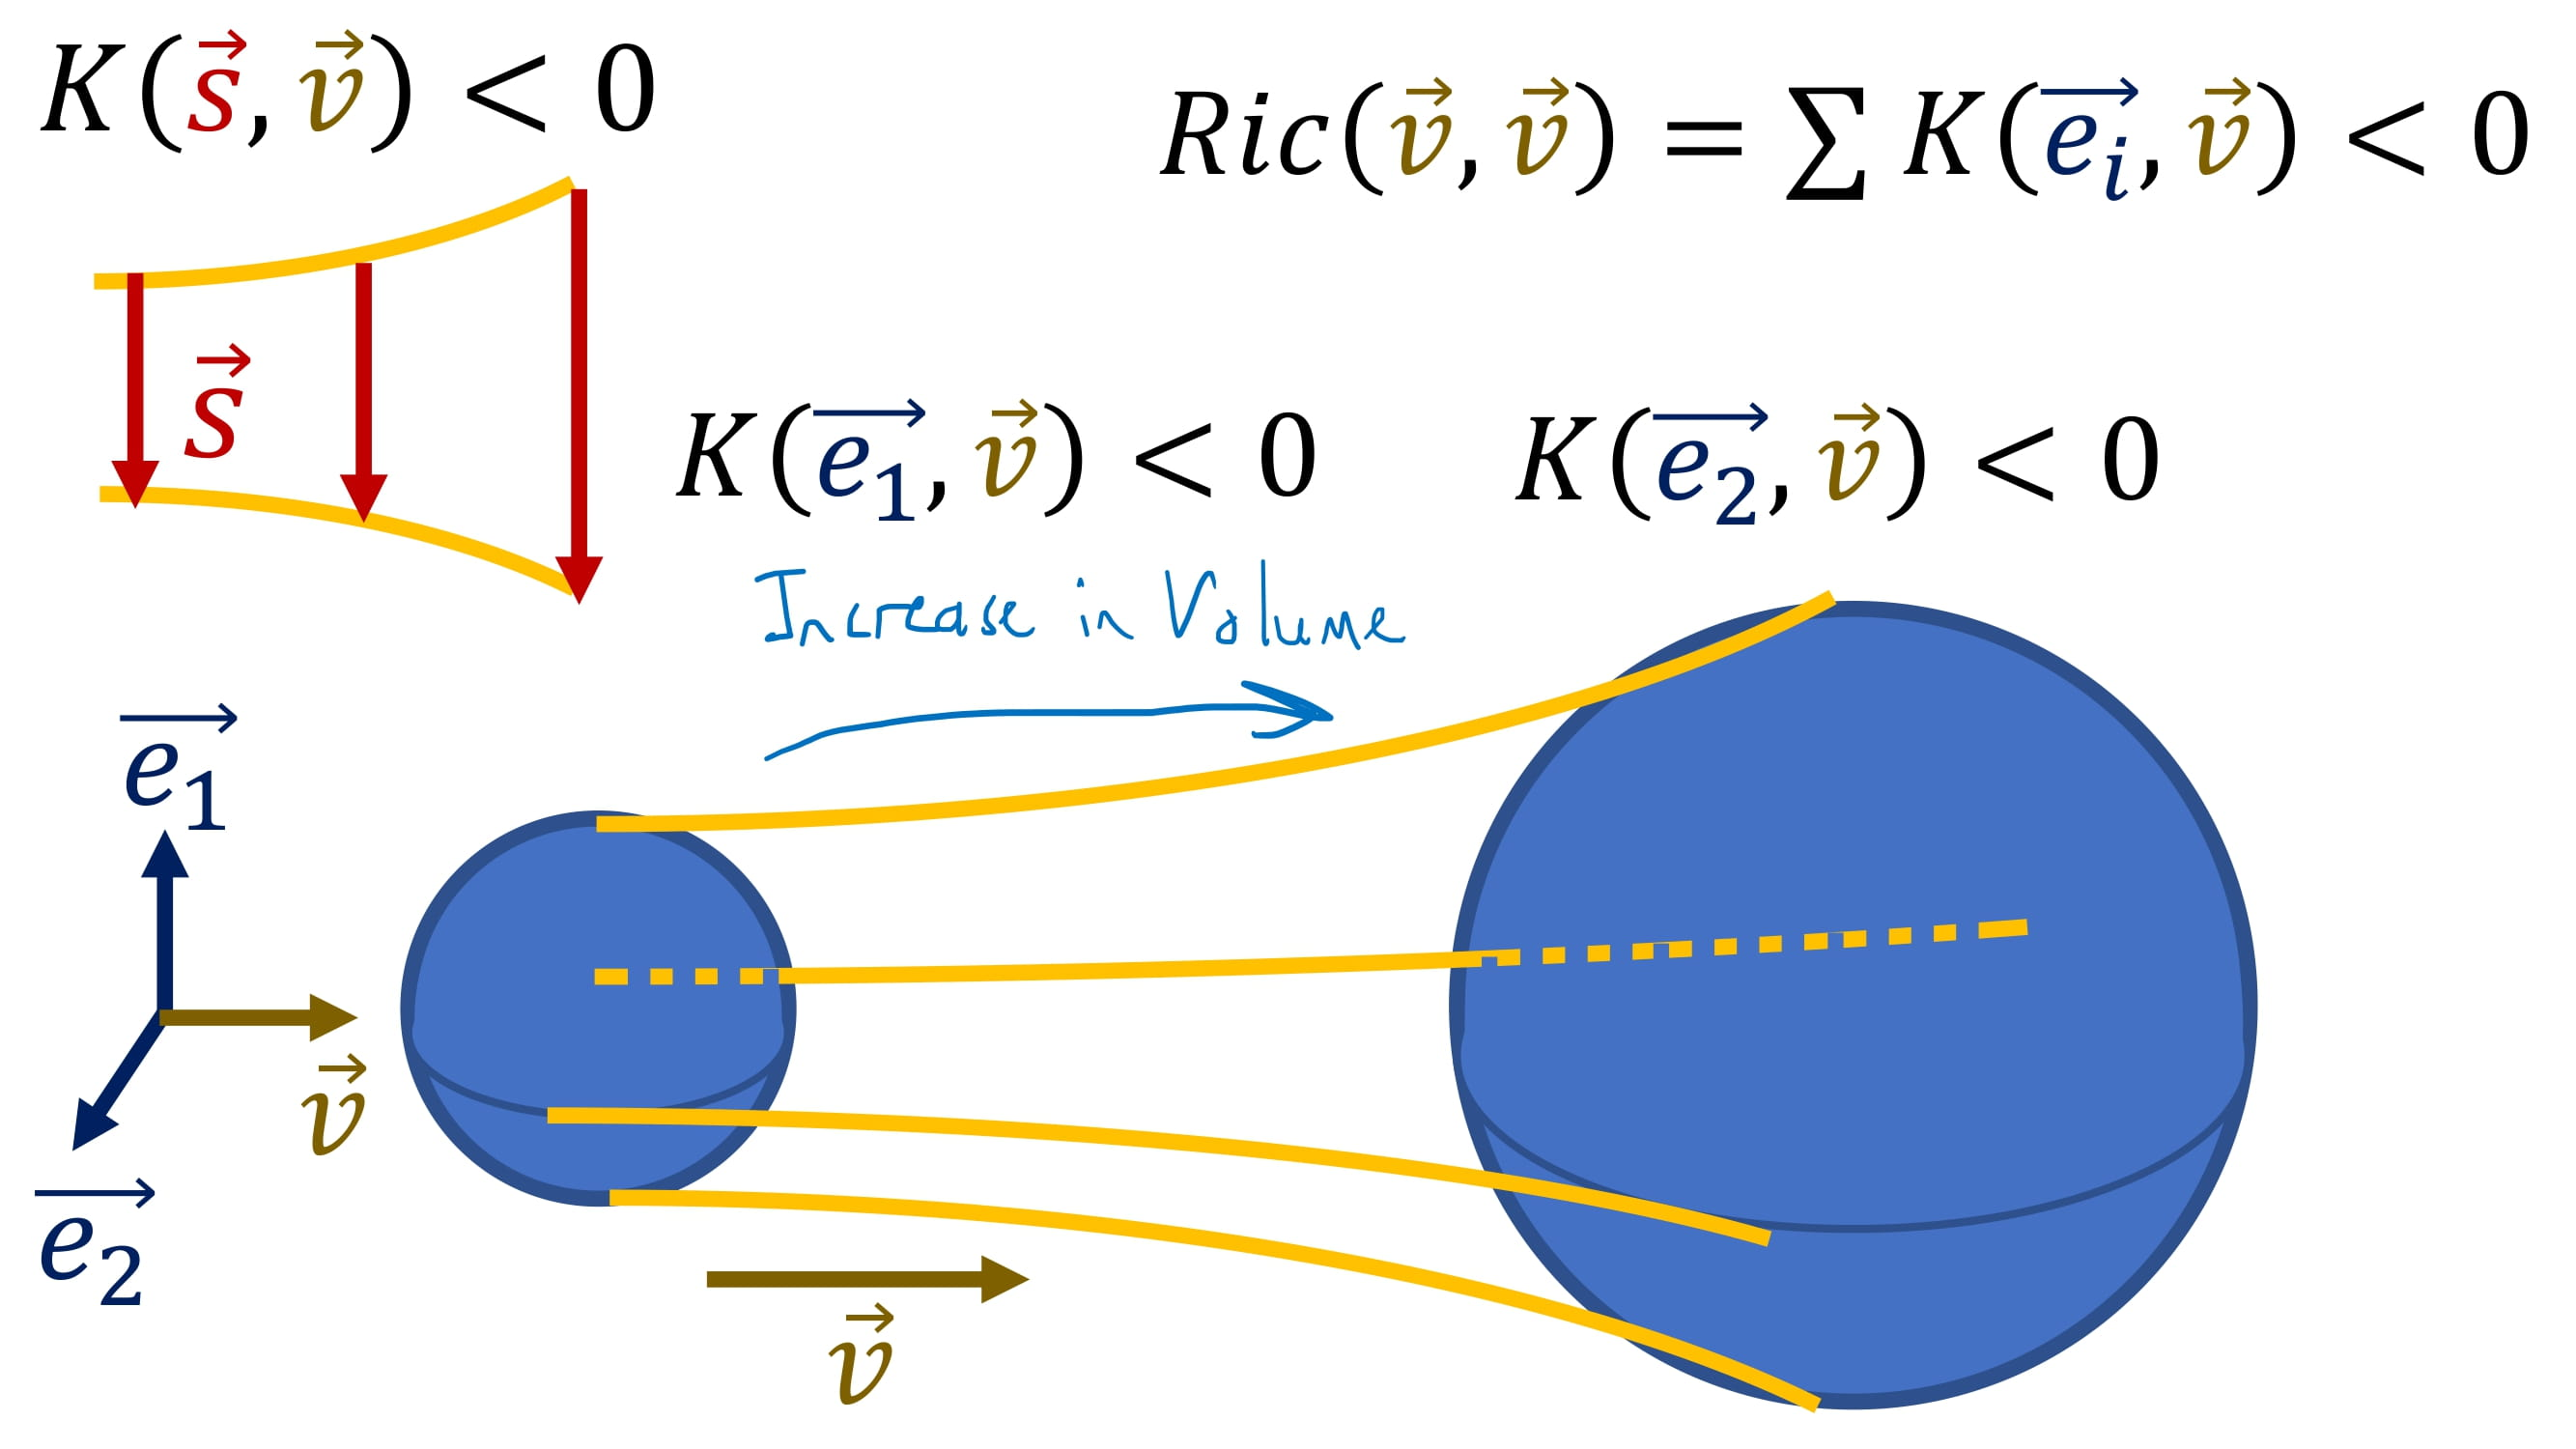
\includegraphics[width=\textwidth]{Figs/r3.jpg}
     \end{subfigure}
      \begin{subfigure}[b]{0.245\textwidth}
         \centering
         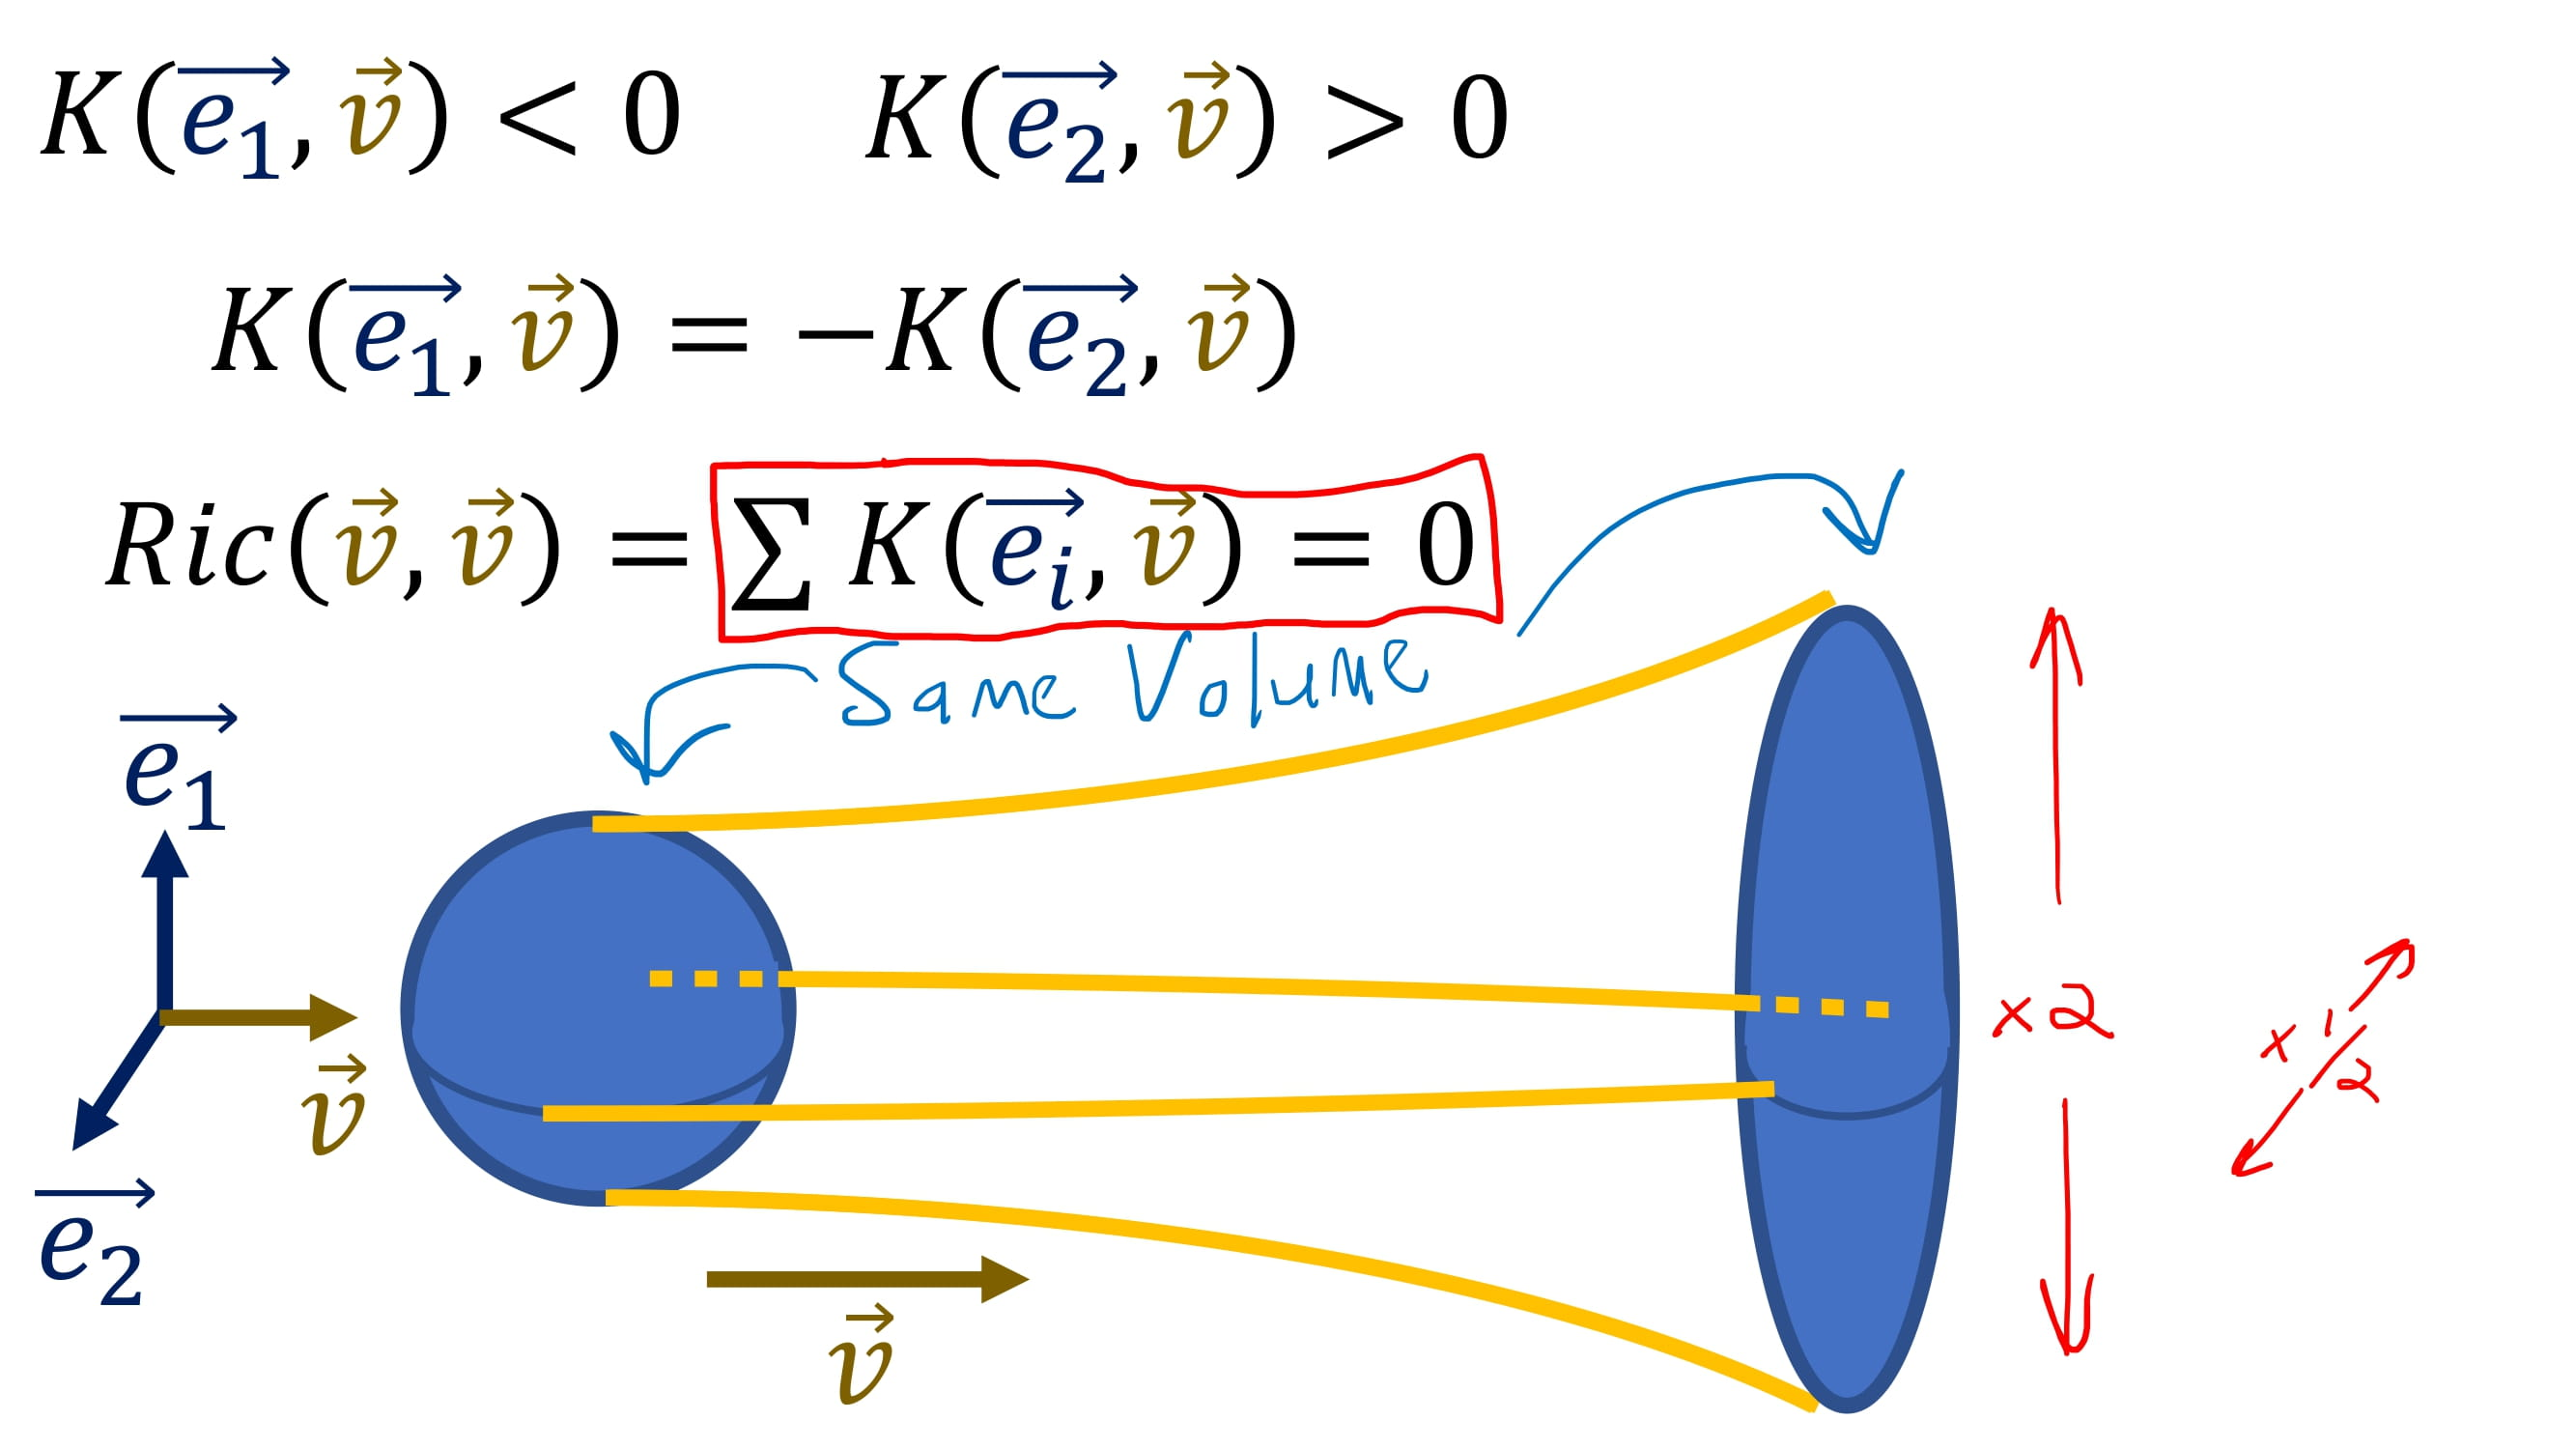
\includegraphics[width=\textwidth]{Figs/r4.jpg}
     \end{subfigure}}
     \caption{\small Ball volume change with different sectional curvatures.} \label{fig:fdfa5er}
\end{figure}
    \item \tb{general volume element derivative:} Ricci tensor tells us how volumes change due to the curvature of the space we are in. See \cref{fig:rjffsf} and \cref{fig:fmamfna}
    \begin{figure}[H]
     \centering
     \makebox[\textwidth][c]{
     \begin{subfigure}[b]{0.49\textwidth}
         \centering
         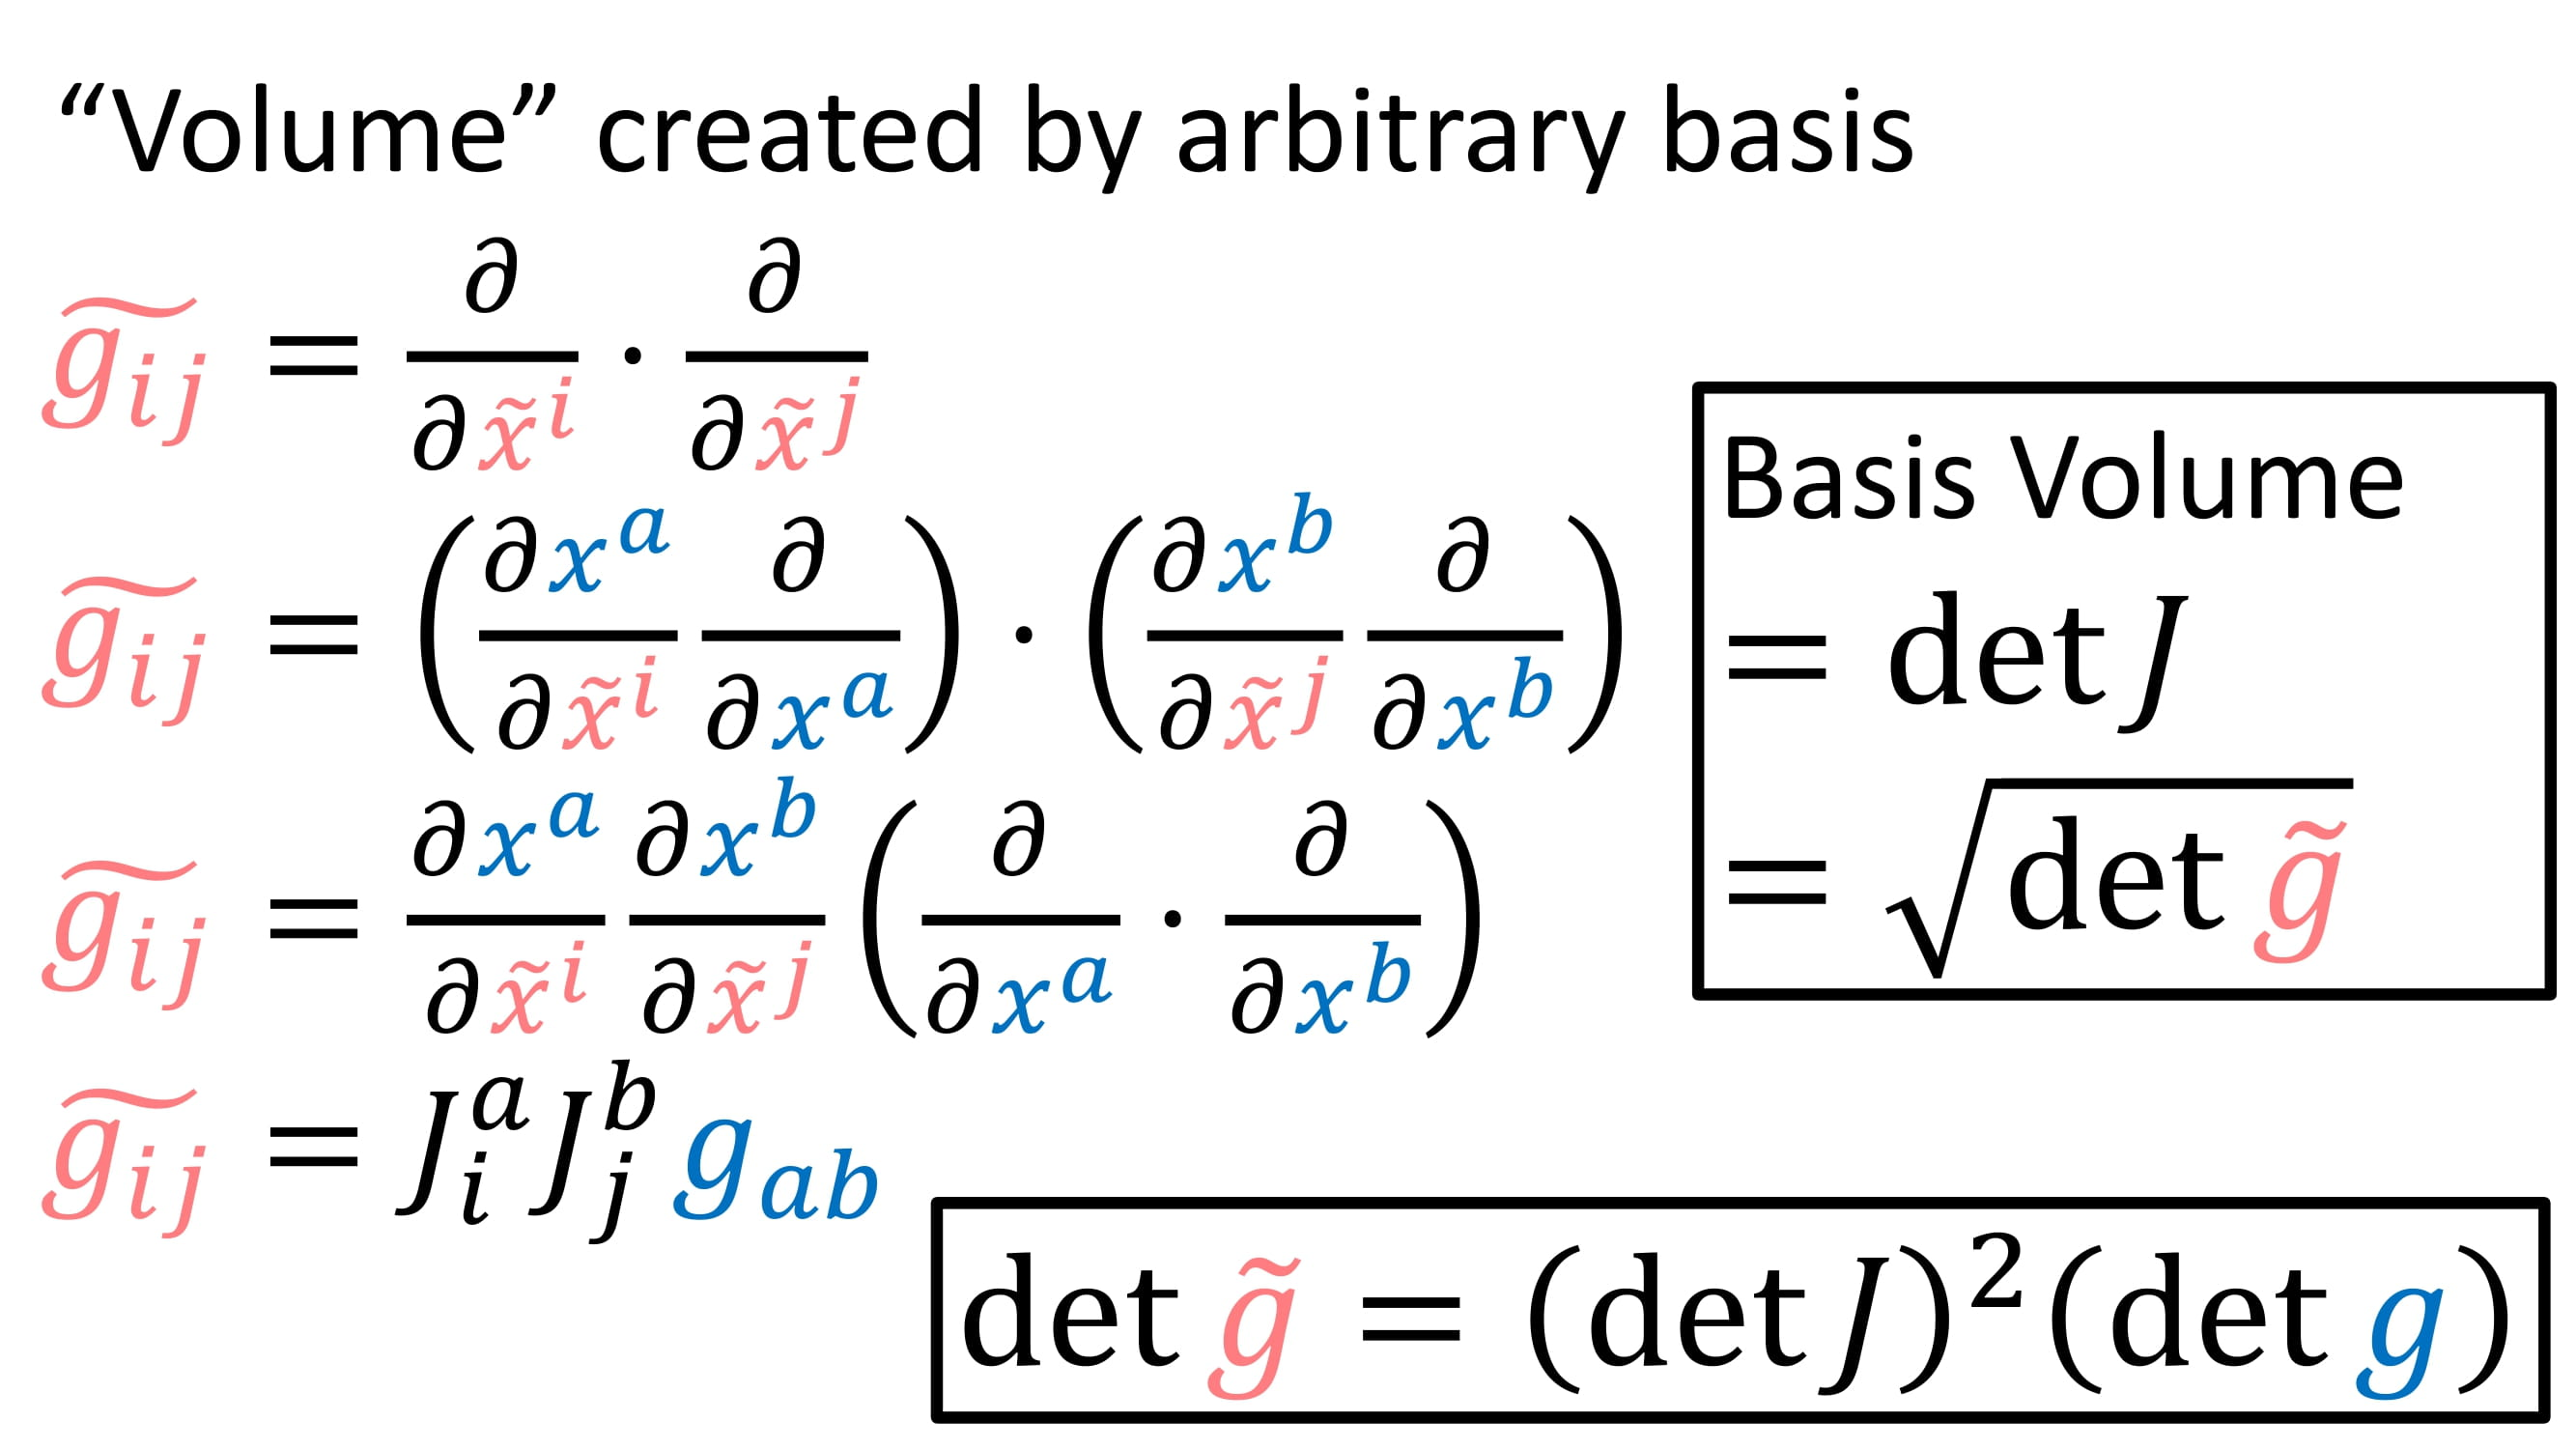
\includegraphics[width=\textwidth]{Figs/v1.jpg}
     \end{subfigure}
      \begin{subfigure}[b]{0.49\textwidth}
         \centering
         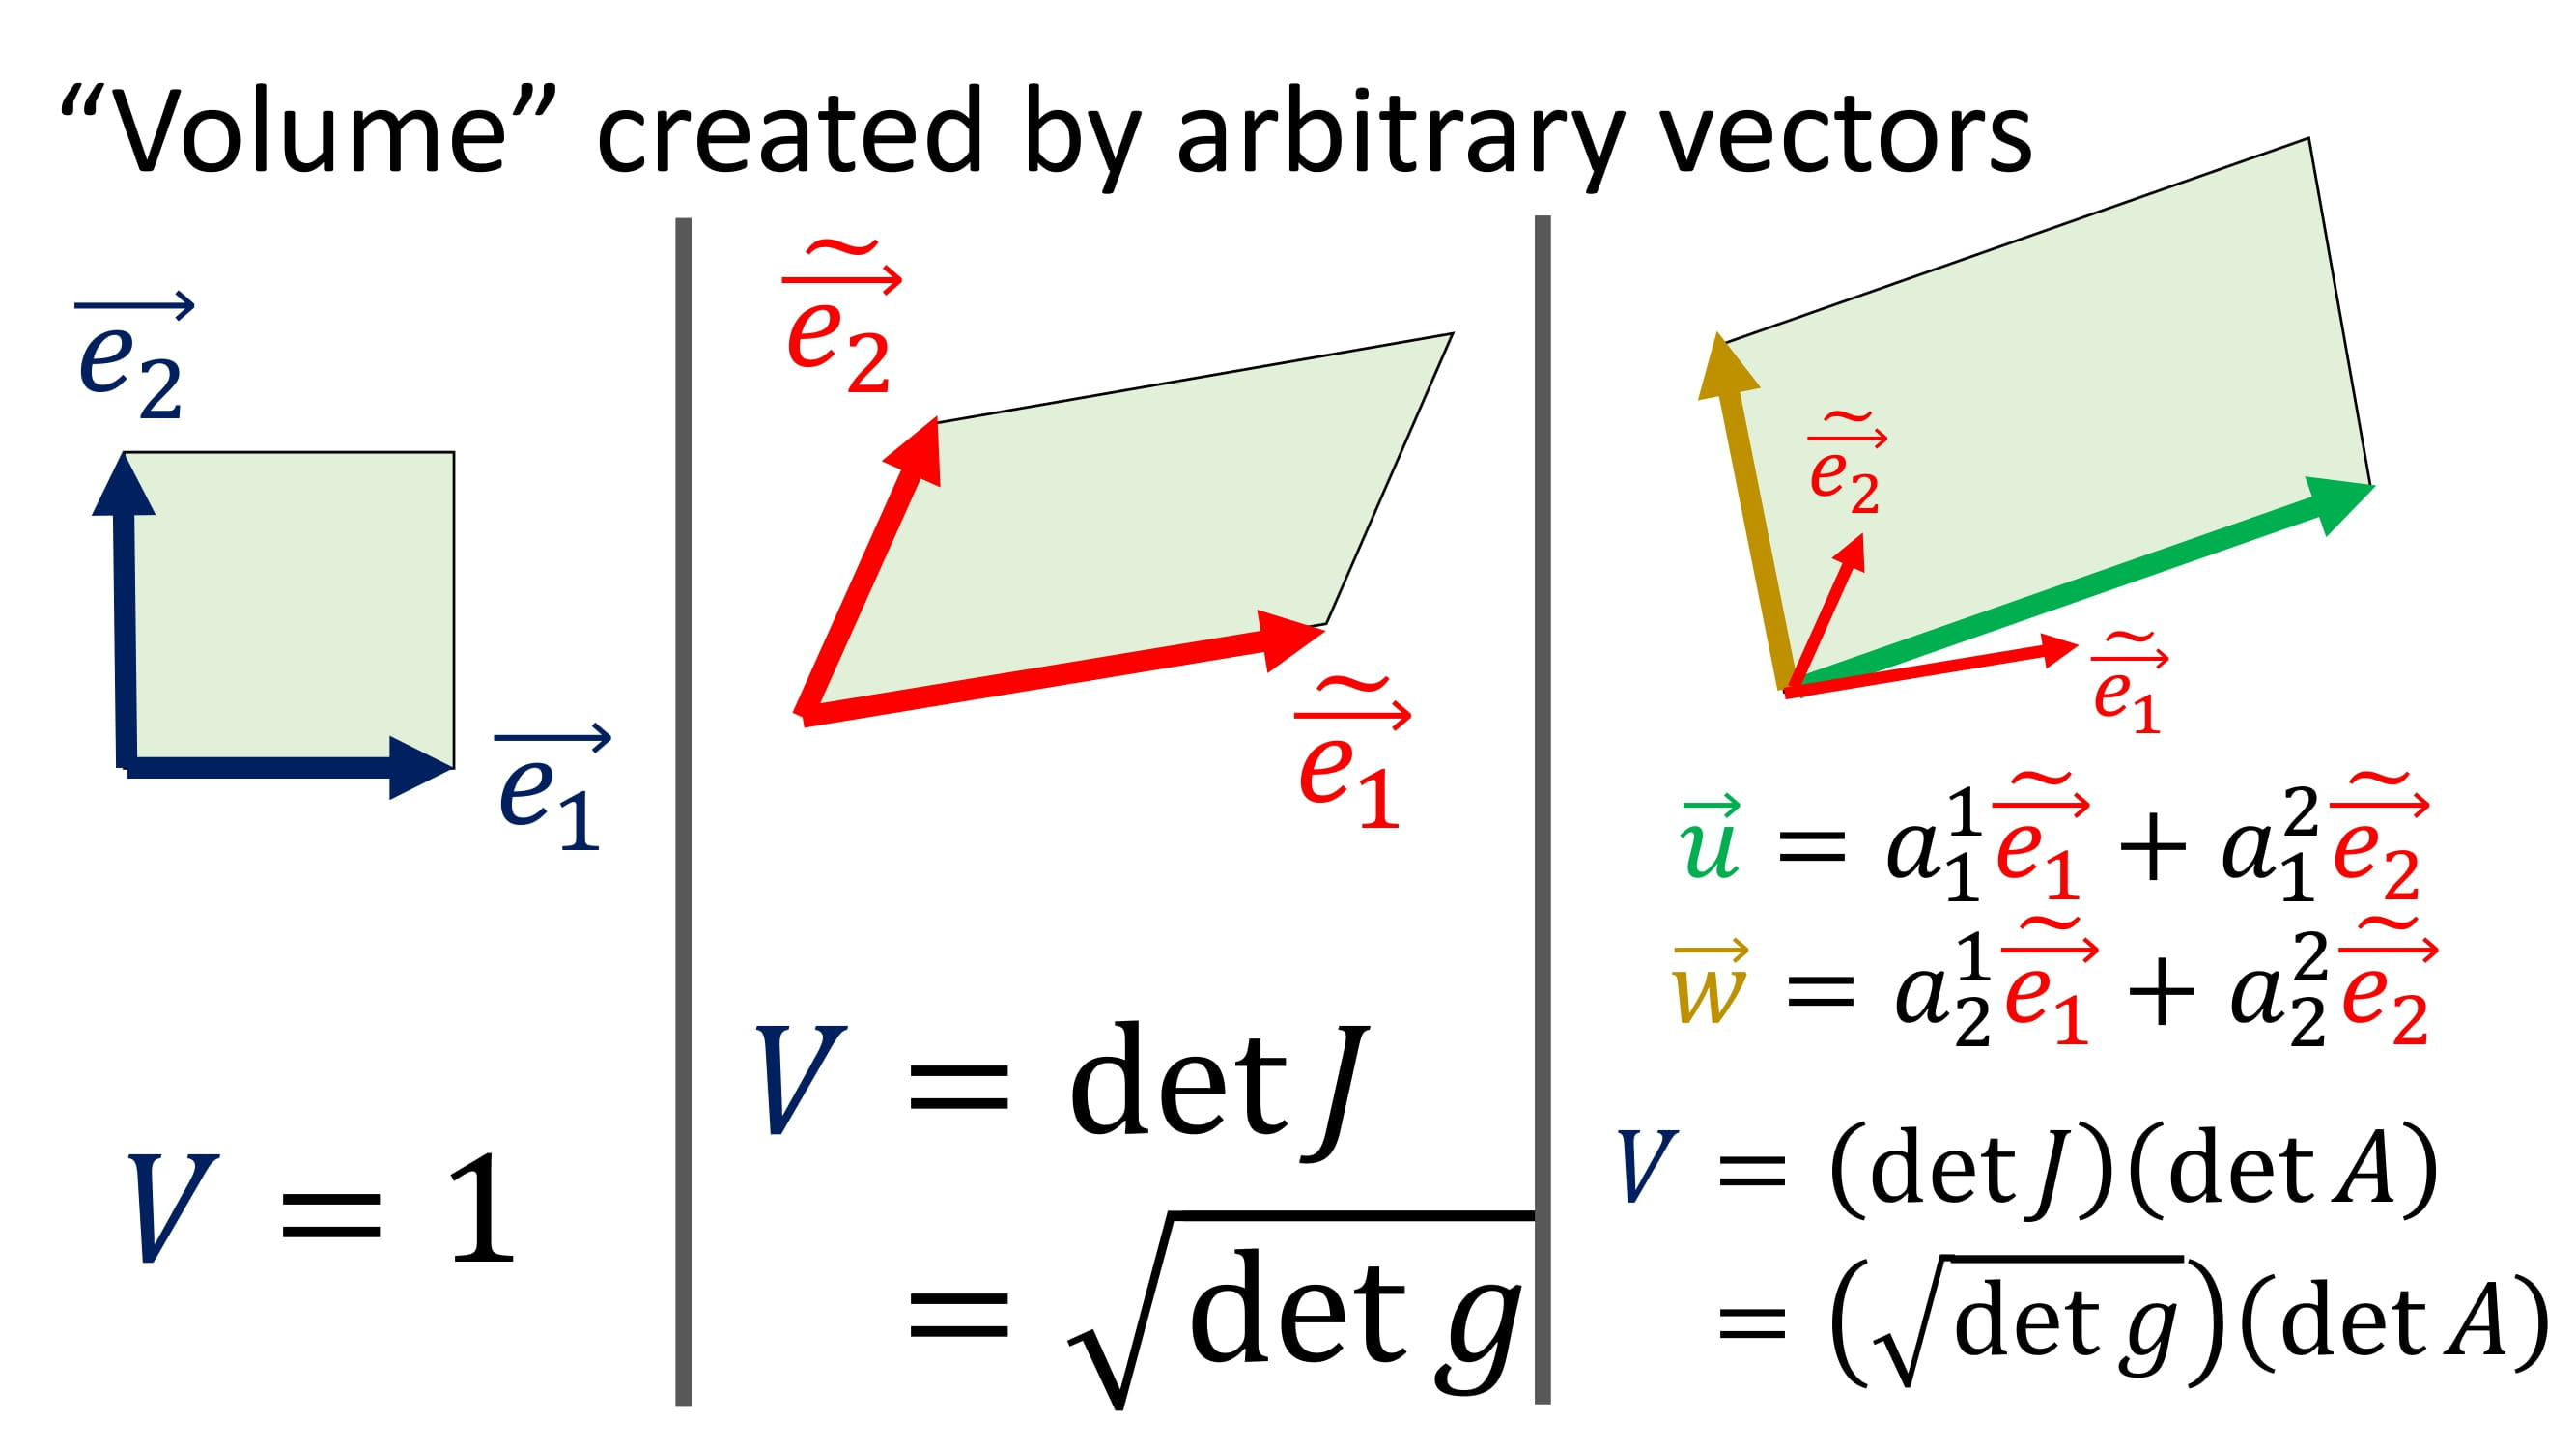
\includegraphics[width=\textwidth]{Figs/v2.jpg}
     \end{subfigure}}
     \caption{\small volume, metric and determinant.} \label{fig:rjffsf}
\end{figure}    
    \begin{figure}[H]
     \centering
     \makebox[\textwidth][c]{
     \begin{subfigure}[b]{0.33\textwidth}
         \centering
         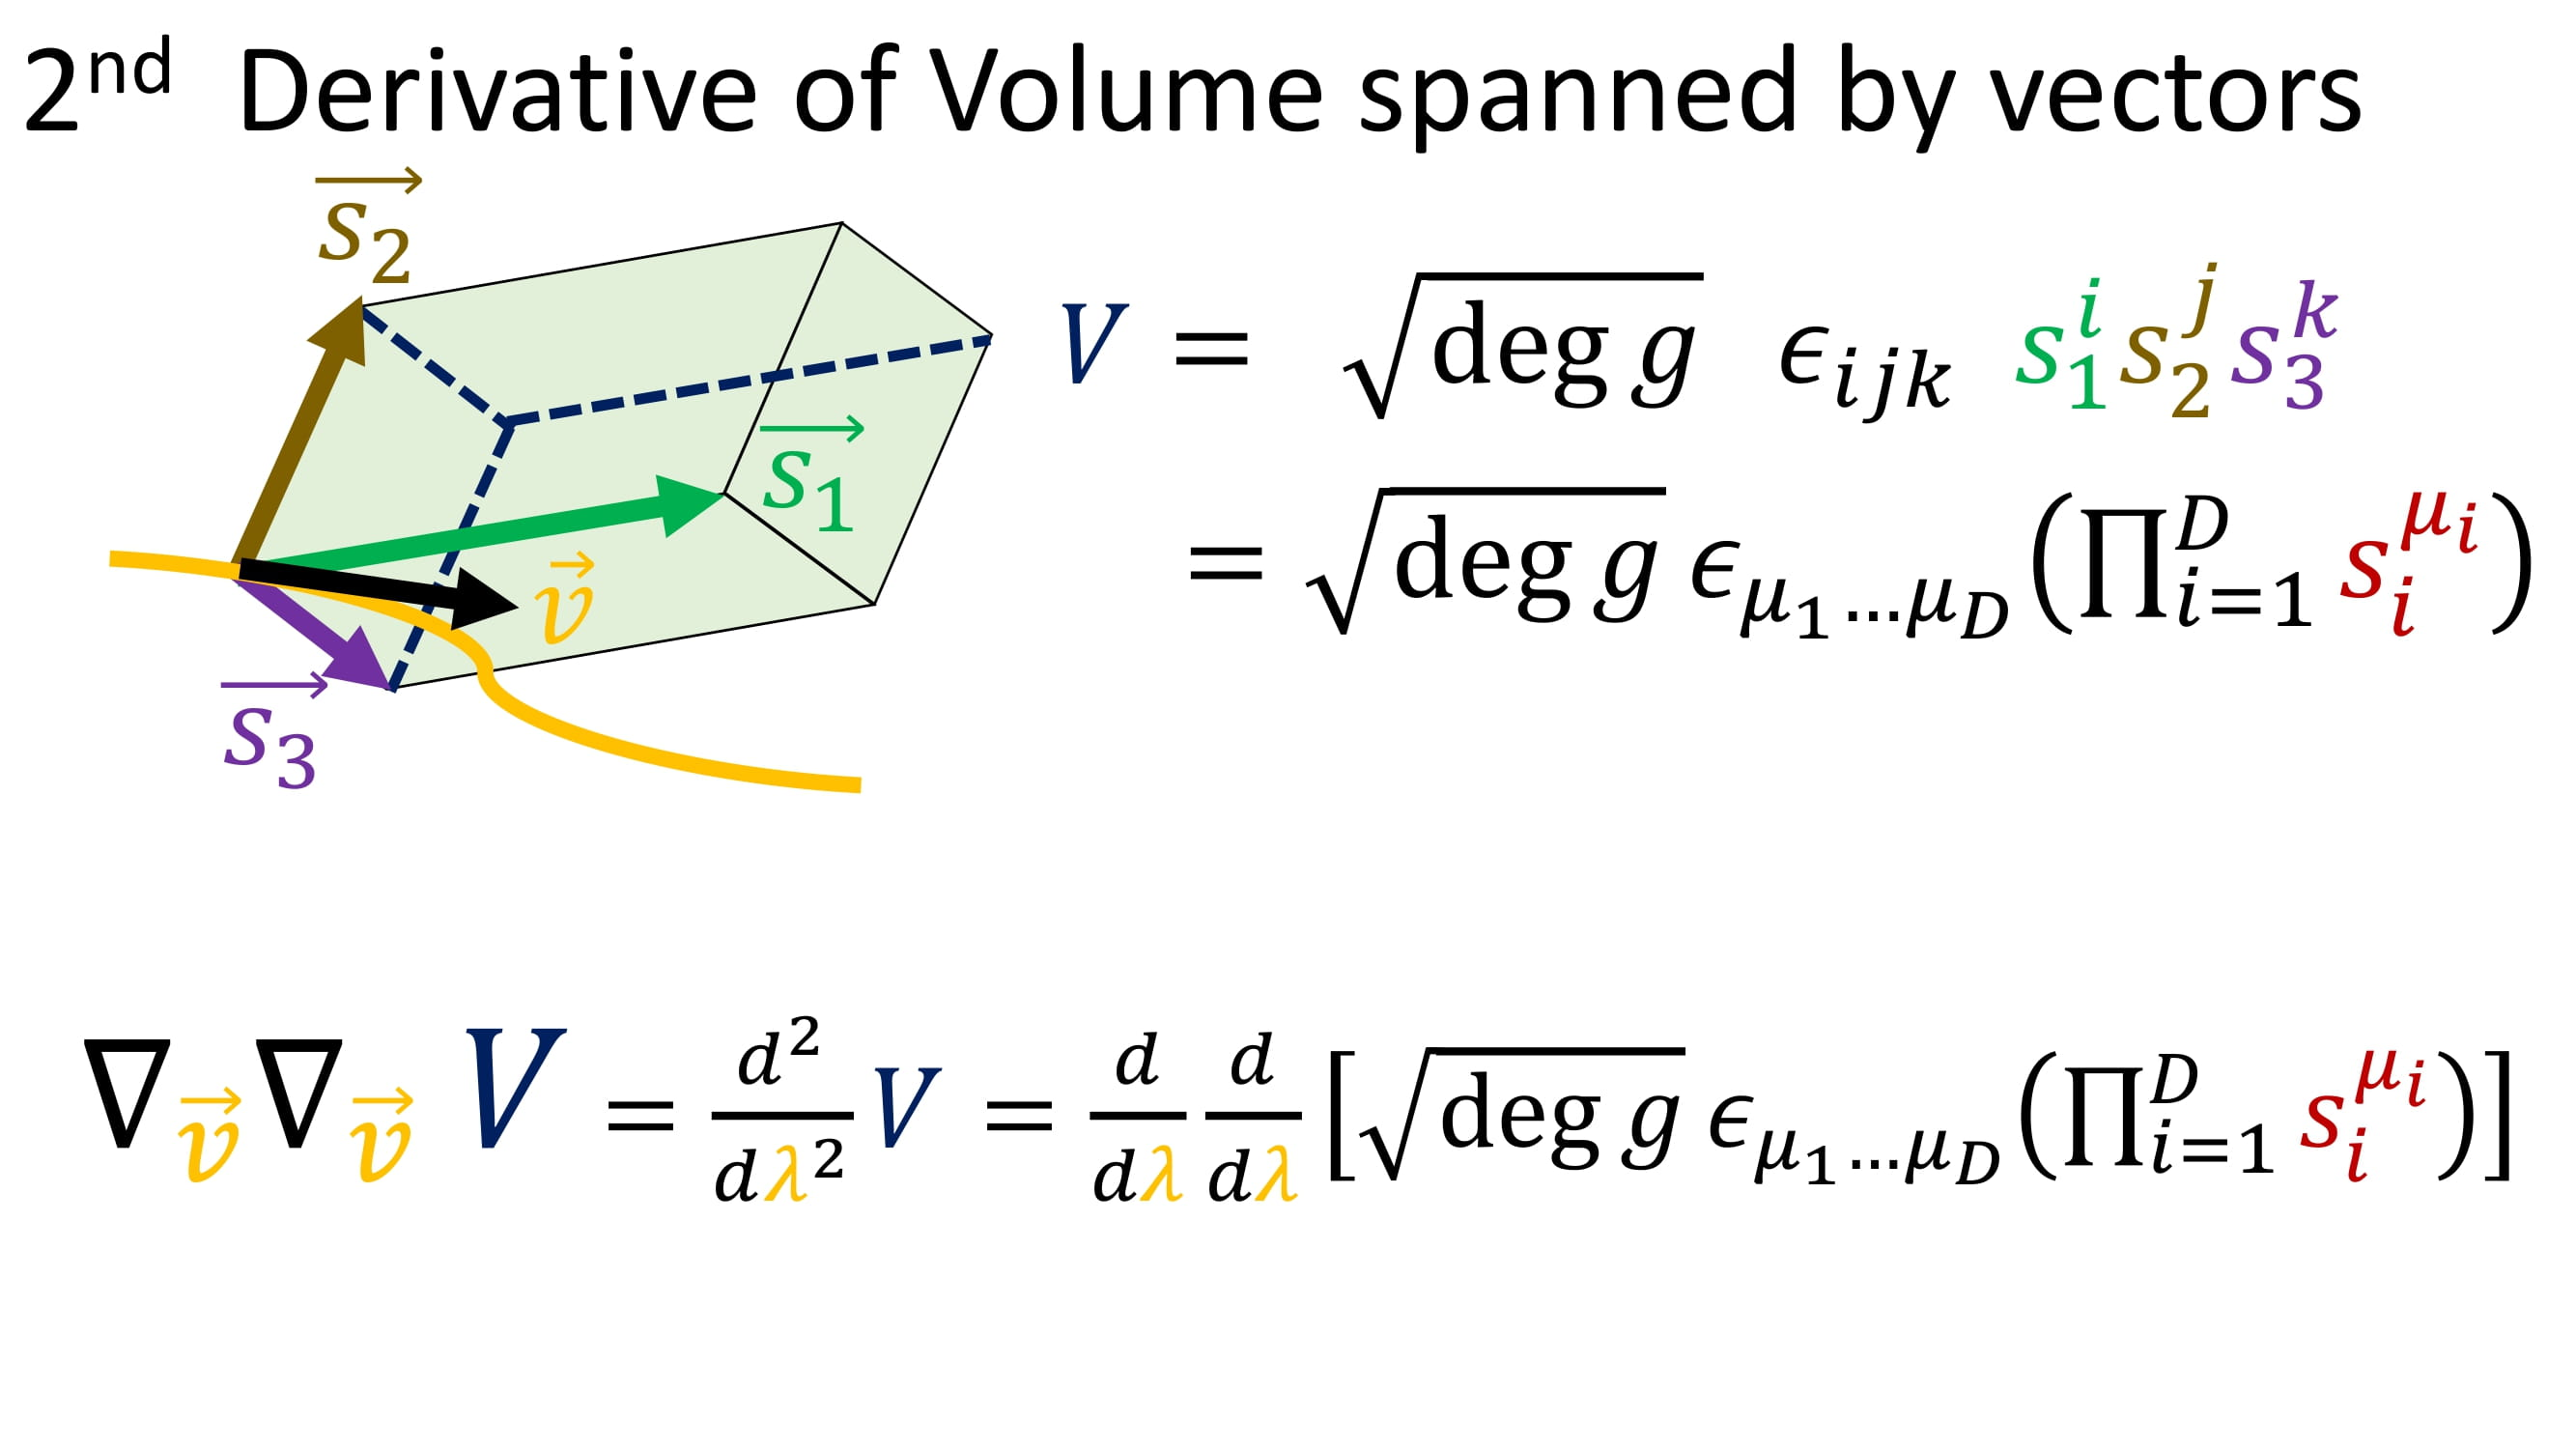
\includegraphics[width=\textwidth]{Figs/v3.jpg}
     \end{subfigure}
     \hfill
     \begin{subfigure}[b]{0.33\textwidth}
         \centering
         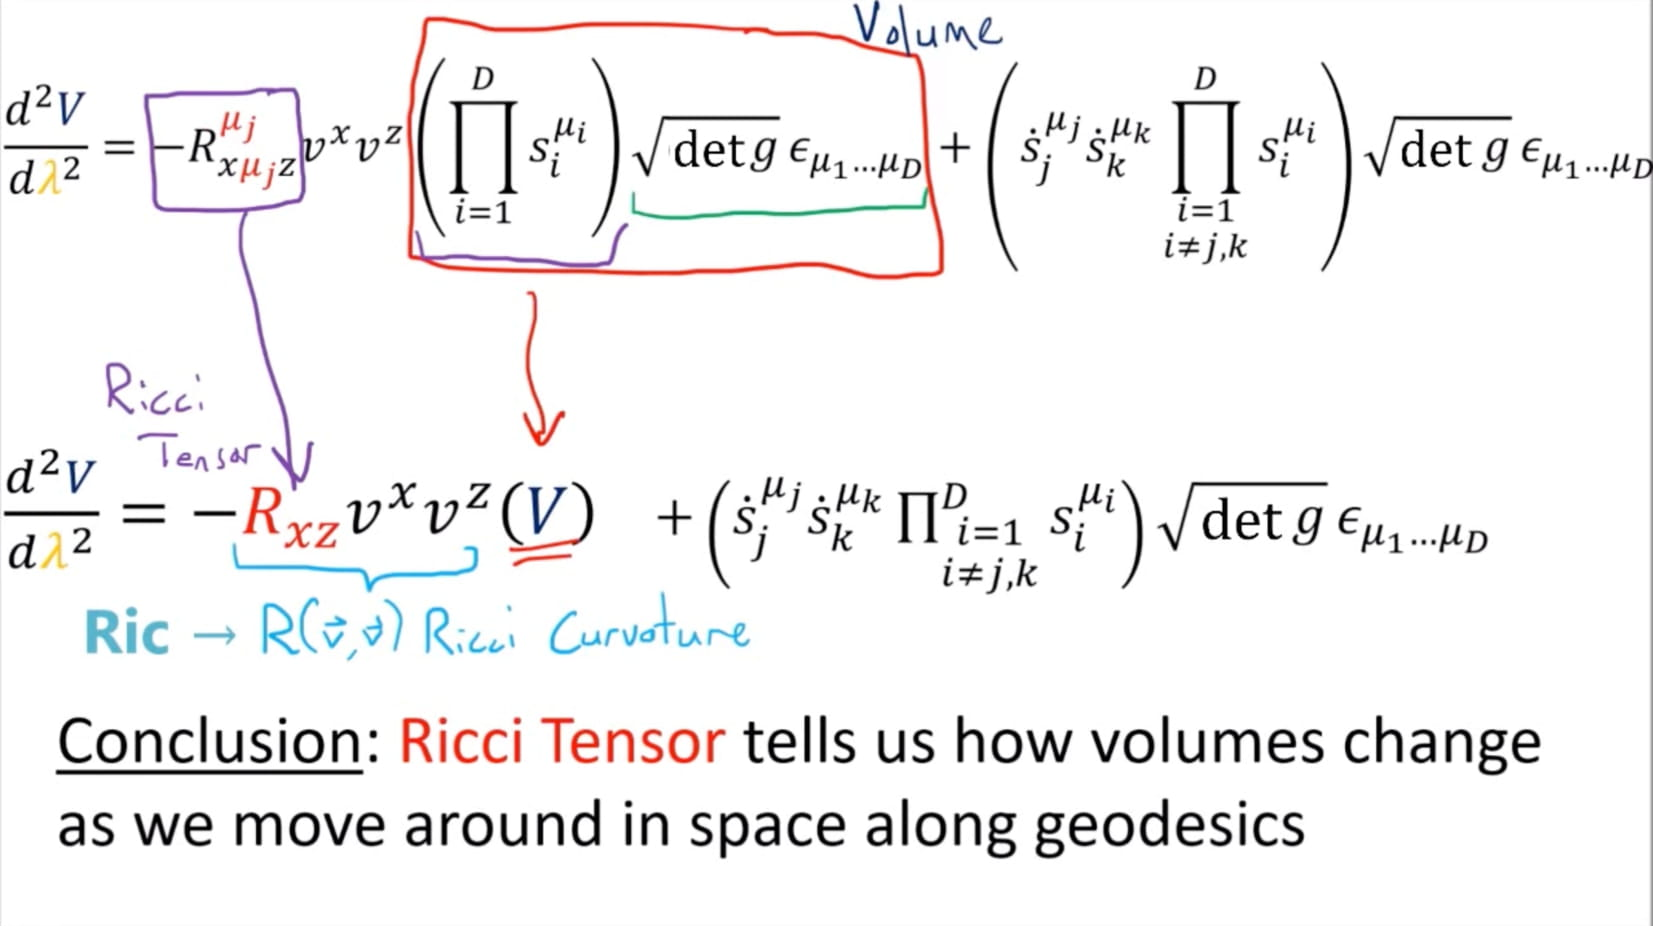
\includegraphics[width=\textwidth]{Figs/v4.jpg}
     \end{subfigure}
      \begin{subfigure}[b]{0.33\textwidth}
         \centering
         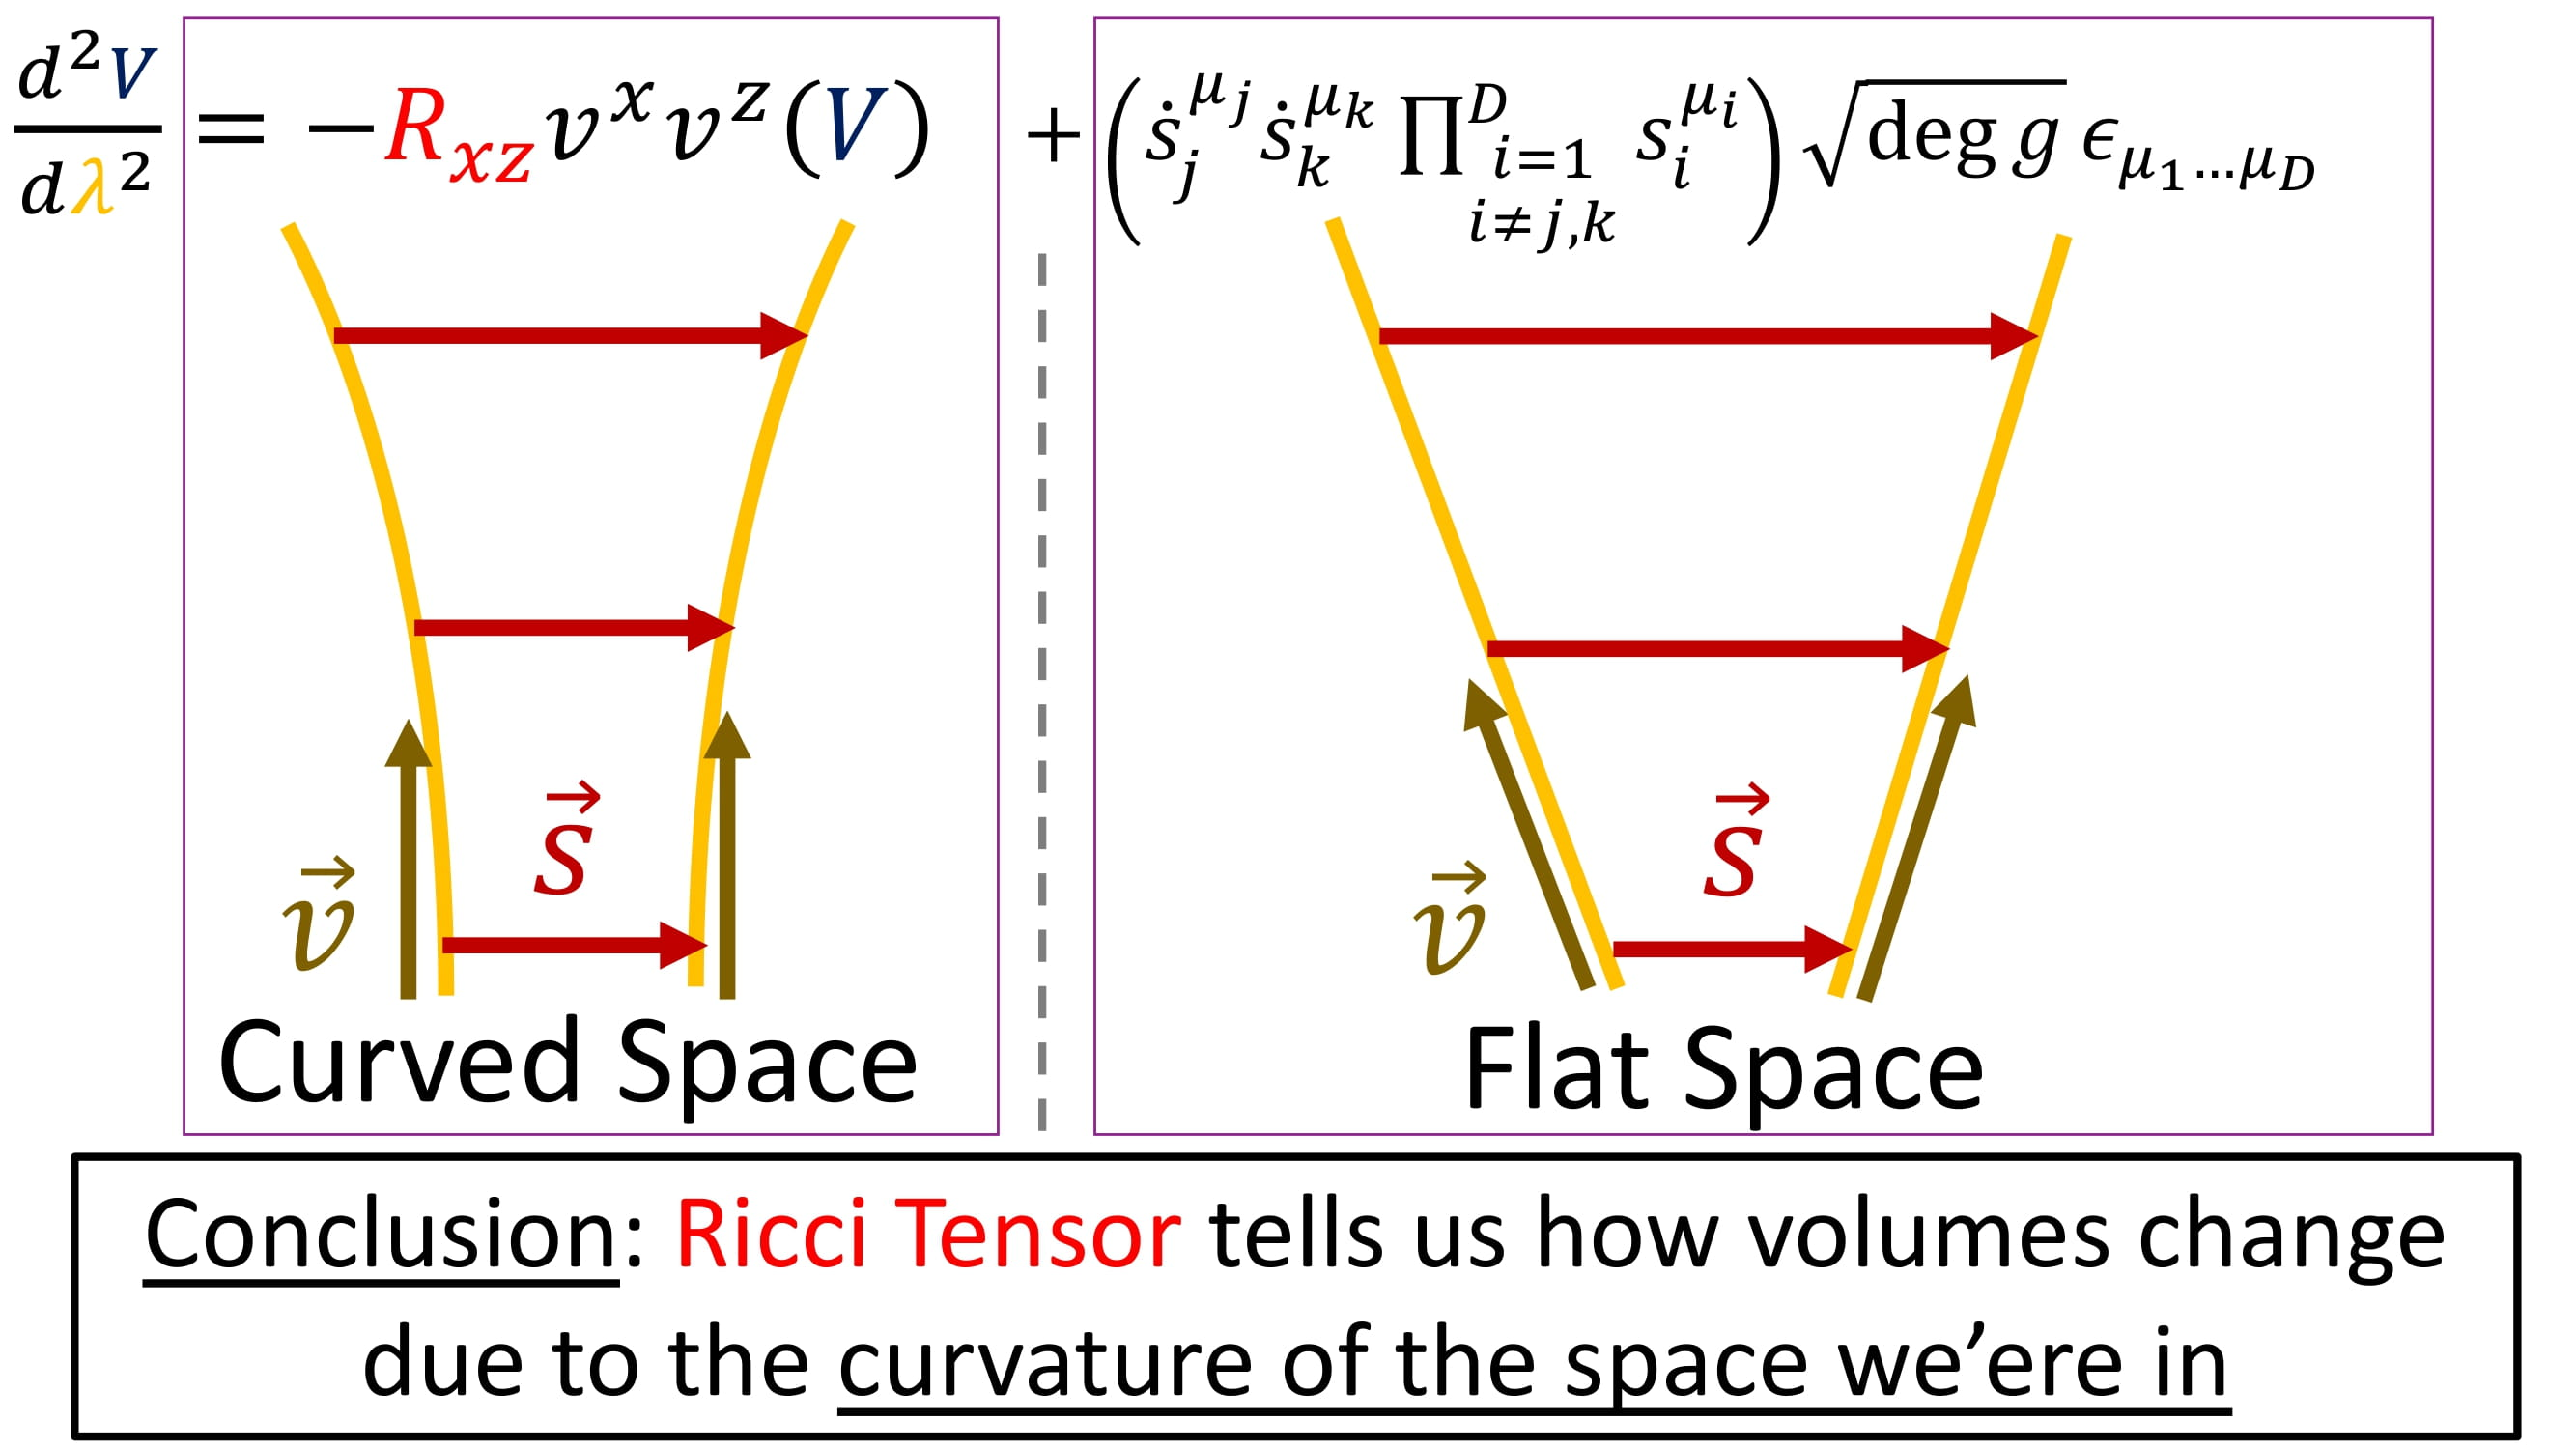
\includegraphics[width=\textwidth]{Figs/v5.jpg}
     \end{subfigure}}
     \caption{\small volume, metric and determinant.} \label{fig:fmamfna}
\end{figure}
    \end{enumerate}
    \item  \tb{Ricci scalar:} To each point on a Riemannian manifold, it assigns a single real number determined by the intrinsic geometry of the manifold near that point. Specifically, the scalar curvature represents the amount by which \tb{the volume of a small geodesic ball in a Riemannian manifold deviates from that of the standard ball in Euclidean space.} In two dimensions, the scalar curvature is twice the Gaussian curvature, and completely characterizes the curvature of a surface. (In more than two dimensions, however, the curvature of Riemannian manifolds involves more than one functionally independent quantity, i.e. we need Riemannian curvature to totally understand the curvature.)
    
    The Ricci scalar curvature $S$ can be obtained as
$$
S=\operatorname{tr}_{g} \Ric.
$$
Note the trace depends on the metric as
$$
S=g^{\mu \nu} \Ric_{\mu \nu}=\Ric_{\mu}^{\mu}
$$
\begin{itemize}
    \item Unlike the Riemann curvature tensor or the Ricci tensor, both of which can be defined for any affine connection, the scalar curvature requires \tb{a metric} of some kind. The metric can be pseudo-Riemannian instead of Riemannian. 
\end{itemize}

We have the following  geometric interpretation: 
\begin{enumerate}
    \item When the scalar curvature is positive at a point, the volume of a small ball about the point has smaller volume than a ball of the same radius in Euclidean space.
    \item On the other hand, when the scalar curvature is negative at a point, the volume of a small ball is larger than it would be in Euclidean space.
\end{enumerate}
\begin{rema}
This can be made more quantitative, in order to characterize the precise value of the scalar curvature $S$ at a point $p$ of a Riemannian $n$-manifold $(M, g)$. Namely, the ratio of the $n$-dimensional volume of a ball of radius $\varepsilon$ in the manifold to that of a corresponding ball in Euclidean space is given, for small $\varepsilon$, by
$$
\frac{\operatorname{Vol}\left(B_{\varepsilon}(p) \subset M\right)}{\operatorname{Vol}\left(B_{\varepsilon}(0) \subset \mathbb{R}^{n}\right)}=1-\frac{S}{6(n+2)} \varepsilon^{2}+O\left(\varepsilon^{4}\right) .
$$
Thus, \tb{the second derivative of this ratio, evaluated at radius $\varepsilon=0$, is exactly minus the scalar curvature divided by $3(n+2)$.}
Boundaries of these balls are $(n-1)$-dimensional spheres of radius $\varepsilon$; their hypersurface measures ("areas") satisfy the following equation:
$$
\frac{\operatorname{Area}\left(\partial B_{\varepsilon}(p) \subset M\right)}{\operatorname{Area}\left(\partial B_{\varepsilon}(0) \subset \mathbb{R}^{n}\right)}=1-\frac{S}{6 n} \varepsilon^{2}+O\left(\varepsilon^{4}\right) .
$$
\end{rema}
\end{enumerate}


\end{document}